%%%%%%%%%%%%%%%%%%%%%%%%%%%%%%%%%%%%%%%%%%%%%%%%%%%
%% LaTeX book template                           %%
%% Author: Amber Jain                            %%
%% Modified for Software Engineering Project     %%
%%%%%%%%%%%%%%%%%%%%%%%%%%%%%%%%%%%%%%%%%%%%%%%%%%%

\documentclass[a4paper,11pt,oneside]{book}

% ============================================================
% PACKAGE
% ============================================================

\usepackage[T1]{fontenc}
\usepackage[utf8]{inputenc}

% Font tiếng Việt
\usepackage[T5]{fontenc}
\usepackage{vntex}
\usepackage{lmodern}
\usepackage{longtable}
\usepackage{amssymb}
\usepackage{array}

\usepackage{hyperref}
\usepackage{graphicx}
\usepackage[english]{babel}
\usepackage{float}
\usepackage{xcolor}
\usepackage{tikz}
\setlength{\parindent}{0pt}

% ============================================================
% TÊN CÁC PHẦN TRONG MỤC LỤC
% ============================================================

\addto\captionsenglish{%
	\renewcommand{\contentsname}{Mục lục}
	\renewcommand{\listfigurename}{Danh sách hình}
	\renewcommand{\listtablename}{Danh sách bảng}
}

% ============================================================
% DEDICATION ENVIRONMENT
% ============================================================

\newenvironment{dedication}
{
	\cleardoublepage
	\thispagestyle{empty}
	\vspace*{\stretch{1}}
	\hfill\begin{minipage}[t]{0.66\textwidth}
		\raggedright
	}
	{
	\end{minipage}
	\vspace*{\stretch{3}}
	\clearpage
}

% ============================================================
% CHAPTER QUOTE
% ============================================================

\makeatletter

\renewcommand{\@chapapp}{}

\newenvironment{chapquote}[2][2em]
{
	\setlength{\@tempdima}{#1}
	\def\chapquote@author{#2}
	\parshape 1 \@tempdima
	\dimexpr\textwidth-2\@tempdima\relax%
	\itshape
}
{
	\par\normalfont\hfill--\ \chapquote@author
	\hspace*{\@tempdima}\par\bigskip
}

\makeatother

% ============================================================
% TITLE
% ============================================================

\title{
	\Huge \textbf{BÁO CÁO ĐỒ ÁN CÔNG NGHỆ PHẦN MỀM}
	\\
	\huge Nền tảng kết nối cộng đồng nhiếp ảnh phim với các dịch vụ phòng tối và phòng chụp
}

\author{\textsc{Nhóm: [Tên nhóm]}}

% ============================================================
% ĐÁNH SỐ CHAPTER VÀ SECTION
% ============================================================

\renewcommand{\thechapter}{\Roman{chapter}}
\renewcommand{\thesection}{\arabic{section}}
% Hiển thị mục lục đến cấp 3
\setcounter{tocdepth}{3}
\setcounter{secnumdepth}{3}
% ============================================================
% ĐỊNH DẠNG CHAPTER
% ============================================================

\makeatletter

\renewcommand{\@makechapterhead}[1]{%
	\vspace*{30pt}
	{\noindent\huge\bfseries \thechapter.\ #1\par}
	\vspace{30pt}
}

\makeatother

% ============================================================
% DOCUMENT
% ============================================================

\begin{document}
	
	% ============================================================
	% TRANG BÌA
	% ============================================================
	
	\frontmatter
	
	%%%%%%%%%%%%%%%%%%%%%%%%%%%%%%%%%%%%%%%%%%%%%%%%%%%%%%%%%%%%%%%%%%%%%%
% COVER PAGE
%%%%%%%%%%%%%%%%%%%%%%%%%%%%%%%%%%%%%%%%%%%%%%%%%%%%%%%%%%%%%%%%%%%%%%

\begin{titlepage}
	
	% ============================================================
	% VIỀN TRANG
	% ============================================================
	
	\begin{tikzpicture}[remember picture,overlay]
		
		% Viền ngoài
		\draw[color=black, line width=1pt]
		([xshift=0.35cm,yshift=-0.35cm]current page.north west)
		rectangle
		([xshift=-0.35cm,yshift=0.35cm]current page.south east);
		
		% Viền trong
		\draw[color=black, line width=0.5pt]
		([xshift=0.48cm,yshift=-0.48cm]current page.north west)
		rectangle
		([xshift=-0.48cm,yshift=0.48cm]current page.south east);
		
	\end{tikzpicture}
	
	% ============================================================
	% PHẦN ĐẦU TRANG
	% ============================================================
	
	\begin{center}
		
		\vspace*{0.15cm}
		
		{\large\bfseries
			TRƯỜNG ĐẠI HỌC GIAO THÔNG VẬN TẢI TP.HCM
		}
		
		\vspace{0.15cm}
		
		{\large\bfseries
			VIỆN CÔNG NGHỆ THÔNG TIN VÀ ĐIỆN TỬ
		}
		
		% ============================================================
		% LOGO
		% ============================================================
		
		\vspace{0.55cm}
		
		
\includegraphics[
		width=8cm
		]{images/1.jpg}
		
		% ============================================================
		% TÊN ĐỒ ÁN
		% ============================================================
		
		\vspace{0.9cm}
		
		{\Large\bfseries
			ĐỒ ÁN MÔN HỌC
		}
		
		\vspace{0.15cm}
		
		{\Large\bfseries
			CÔNG NGHỆ PHẦN MỀM
		}
		
	\end{center}
	
	% ============================================================
	% TÊN ĐỀ TÀI
	% ============================================================
	\begin{center}
	\vspace{1.25cm}
	
	\noindent
	{\large\bfseries\textcolor{red}{TÊN ĐỀ TÀI: }}
	
		\vspace{0.35cm}
	
		
	\noindent
	{\Large\bfseries\textcolor{red}{
			Platform Connecting the Film Photography
				\vspace{0.30cm}
			\\Community with Darkroom and Studio Services
	}}
	
	% ============================================================
	% THÔNG TIN GIẢNG VIÊN + SINH VIÊN
	% ============================================================
	
	\vspace{1.7cm}


% ============================================================
% THÔNG TIN GIẢNG VIÊN + SINH VIÊN
% ============================================================

\vspace{1.4cm}

\noindent
\hfill
\begin{minipage}[t]{10cm}
	
	{\Large\bfseries GVHD: }{\Large Nguyễn Văn Chiến}
	
	\vspace{0.35cm}
	
	{\Large\bfseries Sinh viên thực hiện:}
	
	\vspace{0.30cm}
	
	{\Large 079306043275\_Phạm Thanh Nhàn}
	
	\vspace{0.30cm}
	
	{\Large 082306007566\_Đoàn Minh Thư}
	
	\vspace{0.30cm}
	
	{\Large 080206007896\_Trần Sơn Lâm}
	
	\vspace{0.30cm}
	
	{\Large 22H1320013\_Đặng Lê Quang Cường}
	
	\vspace{0.30cm}
	
\end{minipage}
\end{center}


% ============================================================
% NGÀY THÁNG
% ============================================================




\vspace{1.9cm}

\begin{center}
	{\Large Tp. Hồ Chí Minh, tháng 09 năm 2026}
\end{center}

\end{titlepage}
	
	
	% ============================================================
	% LỜI CẢM ƠN
	% ============================================================
	
	\clearpage
	
	\chapter*{LỜI CẢM ƠN}
	
	\vspace{0.8cm}
	
	\noindent
	Trước hết, nhóm chúng em xin gửi lời cảm ơn chân thành đến Giảng viên bộ môn – thầy Nguyễn Văn Chiến đã tận tình giảng dạy, hướng dẫn và định hướng cho chúng em trong suốt quá trình học tập môn Công nghệ phần mềm.
	
	\vspace{0.4cm}
	
	\noindent
	Những kiến thức và sự hỗ trợ của Thầy đã giúp nhóm có nền tảng cần thiết để thực hiện báo cáo, đồng thời có định hướng rõ ràng trong việc phân tích, thiết kế và phát triển đề tài. Nhóm cũng xin cảm ơn Thầy đã luôn tạo điều kiện thuận lợi, tận tình giải đáp những thắc mắc và hướng dẫn chúng em trong quá trình thực hiện.
	
	\vspace{0.4cm}
	
	\noindent
	Qua quá trình học tập và thực hiện báo cáo, chúng em đã có cơ hội củng cố kiến thức về quy trình phát triển phần mềm, phân tích yêu cầu, thiết kế hệ thống và xây dựng phần mềm. Đây là những kiến thức và trải nghiệm quý giá mà nhóm sẽ ghi nhớ và vận dụng trong quá trình học tập cũng như công việc sau này.
	
	\vspace{0.4cm}
	
	\noindent
	Một lần nữa, nhóm chúng em xin chân thành cảm ơn Thầy và mong rằng sẽ tiếp tục có cơ hội được học hỏi, nhận được sự hướng dẫn và góp ý của Thầy trong những học kỳ tiếp theo.
	
	\vspace{0.5cm}
	
	\begin{flushright}
		\textit{Xin chân thành cảm ơn!}
	\end{flushright}
	
	\clearpage
	
	% ============================================================
	% MỤC LỤC
	% ============================================================
	
	\tableofcontents
	
	\clearpage
	\pagestyle{plain}
	
	% ============================================================
	% DANH SÁCH TỪ VIẾT TẮT
	% ============================================================
	
	\chapter*{DANH SÁCH TỪ VIẾT TẮT}
	
	\vspace{-0.7cm}
	
	\begin{table}[H]
		\hspace*{-1.0cm}
		\small
		\renewcommand{\arraystretch}{1.3}
		
		\begin{tabular}{|c|p{1.3cm}|p{5.5cm}|p{5.0cm}|}
			\hline
			\textbf{STT} & \textbf{Từ viết tắt} & \textbf{Từ đầy đủ} & \textbf{Ý nghĩa} \\
			\hline
			
			1 & API & Application Programming Interface
			& Giao diện lập trình ứng dụng \\
			\hline
			
			2 & CRUD & Create, Read, Update, Delete
			& Tạo, đọc, cập nhật, xóa \\
			\hline
			
			3 & CSS & Cascading Style Sheets
			& Ngôn ngữ định kiểu trang web \\
			\hline
			
			4 & CV & Curriculum Vitae
			& Sơ yếu lý lịch \\
			\hline
			
			5 & DB & Database
			& Cơ sở dữ liệu \\
			\hline
			
			6 & DFD & Data Flow Diagram
			& Sơ đồ luồng dữ liệu \\
			\hline
			
			7 & ERD & Entity Relationship Diagram
			& Sơ đồ quan hệ thực thể \\
			\hline
			
			8 & FR & Functional Requirement
			& Yêu cầu chức năng \\
			\hline
			
			9 & HTML & HyperText Markup Language
			& Ngôn ngữ đánh dấu siêu văn bản \\
			\hline
			
			10 & HTTP & Hypertext Transfer Protocol
			& Giao thức truyền tải siêu văn bản \\
			\hline
			
			11 & HTTPS & Hypertext Transfer Protocol Secure
			& Giao thức truyền tải siêu văn bản an toàn \\
			\hline
			
			12 & JSON & JavaScript Object Notation
			& Định dạng trao đổi dữ liệu \\
			\hline
			
			13 & JWT & JSON Web Token
			& Chuẩn token xác thực \\
			\hline
			
			14 & MySQL & My Structured Query Language
			& Hệ quản trị cơ sở dữ liệu quan hệ \\
			\hline
			
			15 & NFR & Non-functional Requirement
			& Yêu cầu phi chức năng \\
			\hline
			
			16 & OAuth & Open Authorization
			& Giao thức ủy quyền \\
			\hline
			
			17 & REST & Representational State Transfer
			& Kiến trúc truyền trạng thái đại diện \\
			\hline
			
			18 & REST API & Representational State Transfer Application Programming Interface
			& Giao diện lập trình ứng dụng theo kiến trúc REST \\
			\hline
			
			19 & SDD & Software Design Description
			& Tài liệu mô tả thiết kế phần mềm \\
			\hline
			
			20 & SDLC & Software Development Life Cycle
			& Vòng đời phát triển phần mềm \\
			\hline
			
			21 & SQL & Structured Query Language
			& Ngôn ngữ truy vấn có cấu trúc \\
			\hline
			
			22 & SRS & Software Requirements Specification
			& Đặc tả yêu cầu phần mềm \\
			\hline
			
			23 & UC & Use Case
			& Ca sử dụng \\
			\hline
			
		\end{tabular}
	\end{table}
	
	\clearpage
	
	% ============================================================
	% DANH SÁCH HÌNH
	% ============================================================
	
	\listoffigures
	
	\clearpage
	
	% ============================================================
	% DANH SÁCH BẢNG
	% ============================================================
	
	\listoftables
	
	\clearpage
	
	% ============================================================
	% MAIN MATTER
	% ============================================================
	
	\mainmatter
	
	\pagestyle{plain}
	
	% ============================================================
	% CHAPTER I
	% INTRODUCTION
	% ============================================================
	
	\chapter{GIỚI THIỆU}

\section{Tổng quan}

\subsection{Thông tin đồ án}
\begin{itemize}
	\item\textbf{Tên đồ án:} Nền tảng kết nối cộng đồng nhiếp ảnh phim với các dịch vụ phòng tối và phòng chụp 
	\item\textbf{Môn học:} Công nghệ phần mềm 
	\item\textbf{Học kỳ:} Hè / Năm học: 2026
\end{itemize}

\subsection{Thông tin nhóm thực hiện}
\begin{table}[H]
	\centering
	\begin{tabular}{|l|l|l|}
		\hline
		\textbf{Họ và tên} & \textbf{Vai trò} & \textbf{Email} \\
		\hline
		Phạm Thanh Nhàn & Nhóm trưởng & nahnht203@gmail.com \\
		\hline
		Đoàn Minh Thư & Thành viên & thu1106877@gmail.com \\
		\hline
		Đặng Lê Quang Cường & Thành viên & 22h1320013@ut.edu.vn  \\
		\hline
		Trần Sơn Lâm & Thành viên & lamts7896@ut.edu.vn\\
		\hline
	\end{tabular}
	\caption{Danh sách thành viên nhóm thực hiện}
\end{table}

\section{Bối cảnh sản phẩm}

Trong những năm gần đây, nhiếp ảnh phim ngày càng thu hút sự quan tâm của cộng đồng yêu thích nghệ thuật nhiếp ảnh, kéo theo nhu cầu sử dụng phòng tối, studio, thiết bị và các dịch vụ hỗ trợ ngày càng tăng. Tuy nhiên, việc tìm kiếm, đặt chỗ và quản lý các nguồn lực này vẫn còn phân tán, chủ yếu được thực hiện thủ công thông qua mạng xã hội hoặc các kênh liên lạc riêng lẻ, gây mất thời gian và dễ xảy ra sai sót.

Bên cạnh đó, các nhà cung cấp dịch vụ cũng gặp nhiều khó khăn trong việc quản lý không gian, thiết bị, lịch đặt chỗ và hoạt động kinh doanh do thiếu một hệ thống quản lý tập trung. Vì vậy, việc xây dựng một nền tảng tích hợp hỗ trợ kết nối nhiếp ảnh gia với nhà cung cấp dịch vụ, đồng thời ứng dụng trí tuệ nhân tạo để nâng cao trải nghiệm người dùng và tối ưu hóa quản lý là cần thiết.

\section{Các hệ thống hiện có}
\textbf{Giggster} là một marketplace trực tuyến kết nối chủ không gian (studio, phòng chụp, phòng dựng cảnh, địa điểm quay phim...) với người thuê theo giờ hoặc theo ngày. Nền tảng có các đặc điểm đáng chú ý:

\begin{itemize}
	\item \textbf{Tìm kiếm \& lọc:} cho phép người dùng tìm studio theo thành phố, lọc theo mức giá, loại hoạt động và tính năng không gian.
	\item \textbf{Đặt chỗ tức thời:} hỗ trợ đặt chỗ nhanh chỉ với vài thao tác, cùng chính sách hủy miễn phí trong 24 giờ nếu buổi chụp còn cách ít nhất hai ngày.
	\item \textbf{Bảo hiểm/bảo vệ giao dịch:} cung cấp gói bảo hiểm trách nhiệm tùy chọn để bảo vệ ê-kíp và khách hàng trong quá trình sử dụng không gian.
	\item \textbf{Mô hình doanh thu:} thu hoa hồng trên mỗi lượt đặt chỗ thành công (khoảng 19\%) để trang trải chi phí vận hành, phát triển và hỗ trợ nền tảng.
	\item \textbf{Quy mô:} sở hữu hàng nghìn không gian cho thuê tại nhiều thành phố, phục vụ đa dạng nhu cầu từ chụp ảnh sản phẩm, thời trang đến quay phim thương mại.
\end{itemize}

\textbf{Hạn chế của Giggster:}

\begin{itemize}
	\item Không chuyên biệt cho nhiếp ảnh phim (không hỗ trợ đặt phòng tối, thuê máy phim, hóa chất tráng rửa...).
	\item Không có lớp cộng đồng (chia sẻ kỹ thuật, bài viết, workshop).
	\item Không có trợ lý AI hỗ trợ gợi ý hoặc tìm kiếm ngữ nghĩa.
	\item Chưa có mặt tại thị trường Việt Nam.
\end{itemize}

Tại thị trường Việt Nam, chưa có nền tảng tương tự chuyên biệt cho nhiếp ảnh phim; việc tìm và đặt phòng tối, studio hay thuê thiết bị hiện chủ yếu diễn ra qua các hội/nhóm Facebook, trang cá nhân/fanpage của từng studio, hoặc Google Form/Zalo để nhận yêu cầu đặt chỗ và xử lý thủ công.

\section{Thị trường ngách chưa được khai thác}
 

\begin{itemize}
	\item Nhiếp ảnh phim đang trở lại, tạo nhu cầu về studio, phòng tối và thiết bị chuyên dụng.
	\item Phân mảnh trong quản lý phía cung cấp: Hỗ trợ nhà cung cấp quản lý không gian, thiết bị, giá, đặt chỗ và doanh thu trên một nền tảng.
	\item Hiệu ứng mạng: Kết nối nhiếp ảnh gia và nhà cung cấp, kết hợp cộng đồng qua bài viết, đánh giá và workshop.
	\item Lợi thế từ AI: Gợi ý và tìm kiếm thông minh giúp người dùng nhanh chóng tìm được dịch vụ phù hợp.
	\item Khả năng mở rộng doanh thu: Thu phí từ hoa hồng đặt chỗ, gói nâng cao, workshop và vật tư nhiếp ảnh.
\end{itemize}


\section{Tầm nhìn sản phẩm}

Mục tiêu của dự án là xây dựng một nền tảng hỗ trợ cộng đồng nhiếp ảnh phim tìm kiếm và sử dụng các nguồn tài nguyên như phòng tối, studio và thiết bị. Nền tảng giúp người dùng tìm kiếm, đặt chỗ và quản lý lịch sử sử dụng dịch vụ thuận tiện hơn, đồng thời hỗ trợ các nhà cung cấp quản lý không gian và thiết bị. Bên cạnh đó, nền tảng có thêm một số tính năng AI để hỗ trợ tìm kiếm, gợi ý và kết nối người dùng trong cộng đồng nhiếp ảnh phim.

Đối với nhiếp ảnh gia phim và các nhà cung cấp phòng tối, studio, thiết bị, những người đang gặp khó khăn khi tìm kiếm và quản lý dịch vụ, Nền tảng kết nối cộng đồng nhiếp ảnh phim với các dịch vụ phòng tối và phòng chụp là một nền tảng web giúp kết nối người dùng với các dịch vụ nhiếp ảnh phim, giúp tìm kiếm, đặt chỗ và quản lý thông tin sử dụng thuận tiện hơn. Khác với các nhóm mạng xã hội hoặc nền tảng cho thuê không gian nói chung, nền tảng này tập trung vào nhu cầu của cộng đồng nhiếp ảnh phim và có thêm các tính năng AI hỗ trợ tìm kiếm, gợi ý và chia sẻ kiến thức.

\section{Phạm vi và giới hạn đồ án}

\subsection{Các tính năng chính}

\subsubsection{Nhiếp ảnh gia}
\begin{itemize}
	\item FE-01: Đăng ký, đăng nhập và đăng xuất tài khoản.
	\item FE-02: Quản lý hồ sơ cá nhân và thay đổi mật khẩu.
	\item FE-03: Tìm kiếm và xem thông tin chi tiết về không gian sáng tạo, phòng tối và studio.
	\item FE-04: Tạo và quản lý đặt chỗ cho không gian, gói dịch vụ và thiết bị.
	\item FE-05: Xem chi tiết đặt chỗ, trạng thái đặt chỗ và hủy đặt chỗ.
	\item FE-06: Xem hóa đơn và thực hiện thanh toán trực tuyến.
	\item FE-07: Xem lịch sử đặt chỗ và thông tin giao dịch.
	\item FE-08: Xem danh sách workshop, xem chi tiết và đăng ký tham gia workshop.
	\item FE-09: Xem và nhận thông báo liên quan đến tài khoản và hoạt động đặt chỗ.
\end{itemize}

\subsubsection{Nhà cung cấp dịch vụ}
\begin{itemize}
	\item FE-01: Đăng ký, đăng nhập và đăng xuất tài khoản.
	\item FE-02: Quản lý hồ sơ nhà cung cấp dịch vụ.
	\item FE-03: Quản lý không gian sáng tạo, bao gồm thêm, sửa, xóa và cập nhật thông tin không gian.
	\item FE-04: Quản lý thiết bị cho thuê, bao gồm thêm, sửa, xóa và cập nhật thông tin thiết bị.
	\item FE-05: Quản lý gói dịch vụ, bao gồm thông tin gói, giá và các thành phần chi tiết của gói.
	\item FE-06: Quản lý yêu cầu đặt chỗ và xử lý trạng thái đặt chỗ.
	\item FE-07: Xác nhận hoặc từ chối đặt chỗ và thực hiện check-in/check-out cho khách hàng.
	\item FE-08: Quản lý workshop, bao gồm tạo, chỉnh sửa, xóa và xem danh sách người đăng ký.
	\item FE-09: Xem thông tin thanh toán và cập nhật trạng thái thanh toán của các đặt chỗ.
	\item FE-10: Xem dashboard và các thống kê hoạt động kinh doanh.
	\item FE-11: Xem và nhận thông báo liên quan đến hoạt động của nhà cung cấp.
\end{itemize}

\subsubsection{Quản trị viên}
\begin{itemize}
	\item FE-01: Đăng nhập và đăng xuất tài khoản quản trị.
	\item FE-02: Xem và quản lý thông tin người dùng trên hệ thống.
	\item FE-03: Xem, kiểm tra và phê duyệt nhà cung cấp dịch vụ.
	\item FE-04: Xem và giám sát nội dung được quản lý trên nền tảng.
	\item FE-05: Xem và giám sát các giao dịch trên hệ thống.
	\item FE-06: Xem dashboard và các báo cáo, thống kê tổng quan của hệ thống.
	\item FE-07: Quản lý thông tin và thiết lập tài khoản quản trị.
\end{itemize}

\subsection{Giới hạn và phạm vi không triển khai}


\begin{itemize}
	\item LI-01: Không triển khai ứng dụng di động native cho Android hoặc iOS; hệ thống chỉ được phát triển dưới dạng ứng dụng web.
	
	\item LI-02: Không triển khai hệ thống vận chuyển hoặc giao nhận thiết bị giữa nhiếp ảnh gia và nhà cung cấp.
	
	\item LI-03: Không triển khai hệ thống quản lý kho chuyên sâu, bao gồm nhập kho, xuất kho, kiểm kê và quản lý tồn kho tự động.
	
	\item LI-04: Không triển khai hệ thống kế toán và quản lý tài chính chuyên sâu cho nhà cung cấp.
	
	\item LI-05: Không triển khai cơ chế hoàn tiền tự động thông qua cổng thanh toán thực tế.
	
	\item LI-06: Không triển khai hệ thống xác thực danh tính điện tử (KYC) hoặc xác minh giấy tờ pháp lý tự động cho nhà cung cấp.
	
	\item LI-07: Không triển khai chức năng nhắn tin hoặc gọi điện trực tiếp giữa nhiếp ảnh gia và nhà cung cấp.
	
	\item LI-08: Không triển khai mạng xã hội đầy đủ với các chức năng như theo dõi người dùng, nhóm cộng đồng, livestream hoặc nhắn tin riêng.
	
	\item LI-09: Không triển khai mô hình AI chuyên sâu để tự động phục hồi và chỉnh sửa ảnh phim hoàn chỉnh.
	
	\item LI-10: Không triển khai hệ thống kế toán, thuế và báo cáo tài chính chuyên sâu.
	
	\item LI-11: Không triển khai khả năng mở rộng hệ thống ở quy mô thương mại lớn với hàng triệu người dùng và lượng giao dịch cao.
\end{itemize}

	
	% ============================================================
	% CHAPTER II
	% PLAN
	% ============================================================
	
	\chapter{KẾ HOẠCH QUẢN LÝ DỰ ÁN}

\section{Tổng quan}

\subsection{Phạm vi và ước lượng dự án}

Nền tảng kết nối cộng đồng nhiếp ảnh phim với các dịch vụ phòng tối và phòng chụp là một hệ thống web hỗ trợ nhiếp ảnh gia tìm kiếm, đặt chỗ và thanh toán các dịch vụ liên quan đến phòng tối, studio và thiết bị. Hệ thốngổng đồng thời cung cấp các chức năng cho nhà cung cấp quản lý không gian, thiết bị, gói dịch vụ, workshop, đặt chỗ và hoạt động kinh doanh. Ngoài ra, hệ thống hỗ trợ quản trị viên giám sát người dùng, nhà cung cấp và các giao dịch trên nền tảng.

Dự án bao gồm các công việc chính sau:

\setlength{\LTleft}{0pt}
\setlength{\LTright}{0pt}
\renewcommand{\arraystretch}{1.3}

\begin{longtable}{|p{1.0cm}|p{6.0cm}|p{2.5cm}|p{2.5cm}|}
	\caption{\raggedright Cấu trúc phân rã công việc (WBS) và ước lượng công sức}
	\label{tab:wbs}\\
	\hline
	\textbf{WBS} & \textbf{Công việc} & \textbf{Độ phức tạp} &
	\textbf{ngày-người} \\
	\hline
	\endfirsthead
	
	\hline
	\textbf{WBS} & \textbf{Công việc} & \textbf{Độ phức tạp} &
	\textbf{ngày-người} \\
	\hline
	\endhead
	
	1 & Khởi tạo dự án & Trung bình & 4 \\
	\hline
	1.1 & Phân tích yêu cầu và hoàn thiện SRS & Trung bình & 2 \\
	\hline
	1.2 & Thiết lập môi trường, repository và công cụ phát triển & Đơn giản & 2 \\
	\hline
	2 & Phân tích và thiết kế & Trung bình & 8 \\
	\hline
	2.1 & Thiết kế cơ sở dữ liệu & Trung bình & 3 \\
	\hline
	2.2 & Thiết kế kiến trúc hệ thống và API & Trung bình & 2 \\
	\hline
	2.3 & Thiết kế giao diện người dùng & Trung bình & 3 \\
	\hline
	3 & Triển khai hệ thống & Phức tạp & 62 \\
	\hline
	3.1 & Xác thực và quản lý tài khoản & Đơn giản & 5 \\
	\hline
	3.2 & Quản lý hồ sơ người dùng và nhà cung cấp & Đơn giản & 4 \\
	\hline
	3.3 & Quản lý không gian sáng tạo & Trung bình & 8 \\
	\hline
	3.4 & Quản lý thiết bị & Trung bình & 7 \\
	\hline
	3.5 & Quản lý gói dịch vụ & Trung bình & 6 \\
	\hline
	3.6 & Quản lý đặt chỗ và xử lý trạng thái & Phức tạp & 12 \\
	\hline
	3.7 & Thanh toán và hóa đơn & Trung bình & 6 \\
	\hline
	3.8 & Workshop và đăng ký workshop & Trung bình & 5 \\
	\hline
	3.9 & Quản trị hệ thống và dashboard & Trung bình & 5 \\
	\hline
	3.10 & Thông báo và các chức năng hỗ trợ & Đơn giản & 4 \\
	\hline
	
	4 & Kiểm thử & Trung bình & 10 \\
	\hline
	4.1 & Kiểm thử đơn vị & Đơn giản & 3 \\
	\hline
	4.2 & Kiểm thử tích hợp & Trung bình & 4 \\
	\hline
	4.3 & Kiểm thử hệ thống & Trung bình & 3 \\
	\hline
	
	5 & Hoàn thiện và báo cáo & Trung bình & 8 \\
	\hline
	5.1 & Hoàn thiện và kiểm tra hệ thống & Đơn giản & 2 \\
	\hline
	5.2 & Hoàn thiện tài liệu và báo cáo & Trung bình & 6 \\
	\hline
	
\end{longtable}

\setlength{\LTleft}{0pt}
\setlength{\LTright}{0pt}
\renewcommand{\arraystretch}{1.3}

\subsection{Mục tiêu kiểm thử}

\begin{longtable}{|p{3.5cm}|p{6.5cm}|p{4cm}|}
	\caption{\raggedright Mục tiêu kiểm thử}
	\label{tab:testing-objectives}\\
	\hline
	\textbf{Giai đoạn kiểm thử} & \textbf{Phạm vi kiểm thử} & \textbf{Mục tiêu lỗi} \\
	\hline
	\endfirsthead
	
	\hline
	\textbf{Giai đoạn kiểm thử} & \textbf{Phạm vi kiểm thử} & \textbf{Mục tiêu lỗi} \\
	\hline
	\endhead
	
	Rà soát mã nguồn & Kiểm tra quy chuẩn lập trình và cấu trúc mã nguồn & < 10 \\
	\hline
	
	Kiểm thử đơn vị & Kiểm tra các chức năng và xử lý nghiệp vụ riêng lẻ & < 8 \\
	\hline
	
	Kiểm thử tích hợp & Kiểm tra sự kết nối giữa Frontend, Backend, API và cơ sở dữ liệu & < 5 \\
	\hline
	
	Kiểm thử hệ thống & Kiểm tra các luồng chức năng hoàn chỉnh của hệ thống & < 5 \\
	\hline
	
	Kiểm thử chấp nhận & Kiểm tra mức độ đáp ứng các yêu cầu chức năng của người dùng & < 3 \\
	\hline
	
\end{longtable}


\subsection{Các rủi ro dự án}
\setlength{\LTleft}{0pt}
\setlength{\LTright}{0pt}
\renewcommand{\arraystretch}{1.3}

\begin{longtable}{|p{0.6cm}|p{3.5cm}|p{3.5cm}|p{1.8cm}|p{4cm}|}

	\textbf{\#} &
	\textbf{Risk Description} &
	\textbf{Impact} &
	\textbf{Possibility} &
	\textbf{Response Plans} \\
	\hline
	\endhead
	
	1 &
	Timeline gấp (30 ngày) khiến các module core (đặt chỗ, thanh toán) chưa được hoàn thiện đúng hạn. &
	Sản phẩm demo không chạy được luồng chính, ảnh hưởng trực tiếp đến điểm đồ án. &
	High &
	Ưu tiên phát triển các tính năng lõi trước theo MoSCoW, cắt giảm ngay các tính năng phụ (AI, cộng đồng) nếu tiến độ trễ sau tuần 2. \\
	\hline
	
	2 &
	Xác nhận thanh toán qua VietQR được thực hiện thủ công, dễ xảy ra sai sót khi đối chiếu sao kê ngân hàng. &
	Đơn hàng bị xác nhận sai hoặc chậm trễ, gây trải nghiệm không tốt cho người dùng khi demo. &
	Medium &
	Thiết kế rõ trạng thái đơn hàng trung gian (\texttt{waiting\_confirmation}) và kiểm thử kỹ luồng đối chiếu trước khi tích hợp UI. \\
	\hline
	
	3 &
	Chức năng quản lý đặt chỗ và phân bổ tài nguyên (tránh trùng lịch phòng/thiết bị) hoạt động chưa chính xác. &
	Nhiếp ảnh gia có thể đặt trùng lịch với người khác, gây lỗi nghiêm trọng trong luồng chính của hệ thống. &
	High &
	Kiểm thử các trường hợp đặt trùng lịch, kiểm tra logic phân bổ tài nguyên ở Backend và xử lý lỗi rõ ràng trên Frontend. \\
	\hline
	
	4 &
	Tích hợp Frontend và Backend không đồng bộ về API hoặc cấu trúc dữ liệu. &
	Một số chức năng có thể không hiển thị hoặc hoạt động đúng trên giao diện. &
	Medium &
	Thống nhất API endpoint, request/response và kiểm thử API trước khi tích hợp giữa các module. \\
	\hline
	
	5 &
	Thành viên nhóm không hoàn thành task đúng tiến độ hoặc phát sinh xung đột khi merge code. &
	Ảnh hưởng đến tiến độ tích hợp và hoàn thiện hệ thống. &
	Medium &
	Phân chia task rõ ràng trên Jira, sử dụng Git branch riêng và thường xuyên cập nhật tiến độ của từng thành viên. \\
	\hline
	
	6 &
	Các lỗi phát sinh trong quá trình kiểm thử khiến một số chức năng chưa ổn định. &
	Ảnh hưởng đến chất lượng và khả năng hoàn thành bản demo cuối cùng. &
	Medium &
	Thực hiện kiểm thử sớm, ưu tiên sửa các lỗi ảnh hưởng đến chức năng chính và kiểm thử lại sau khi sửa lỗi. \\
	\hline
	
\end{longtable}


\section{Phương pháp quản lý dự án}

\subsection{Quy trình phát triển dự án}

Sau khi xem xét các mô hình phát triển phần mềm, nhóm lựa chọn Quy trình phát triển phần mềm lặp và gia tăng (Iterative and Incremental Software Development Process).

Theo mô hình này, hệ thống được chia thành nhiều phần nhỏ để phát triển từng bước. Sau mỗi vòng lặp, nhóm sẽ hoàn thành một số chức năng, kiểm thử và tiếp tục phát triển các chức năng tiếp theo.

Mô hình này phù hợp với đề tài vì hệ thống có nhiều module khác nhau và các chức năng có liên quan đến nhau. Việc phát triển từng phần giúp nhóm dễ theo dõi tiến độ, kiểm thử và sửa lỗi trong quá trình thực hiện.

Các lý do lựa chọn mô hình này gồm:
\begin{itemize}
	\item Phát triển các chức năng quan trọng trước.
	\item Dễ điều chỉnh khi có thay đổi yêu cầu.
	\item Có thể kiểm thử và sửa lỗi sau mỗi vòng lặp.
	\item Dễ theo dõi tiến độ và quản lý rủi ro.
	\item Có thể cải thiện hệ thống qua từng phiên bản.
\end{itemize}


\subsection{Quản lý chất lượng}

\subsubsection{Phòng ngừa lỗi}

Khi phát hiện lỗi, người phụ trách phải được thông báo ngay. Mỗi lỗi cần được đánh giá về mức độ nghiêm trọng và thời gian cần thiết để xử lý. Các lỗi quan trọng phải được ưu tiên giải quyết và có thời hạn xử lý cụ thể.

Nhóm cũng cần chủ động xác định các vấn đề có thể xảy ra trong quá trình phát triển để có phương án xử lý sớm.

\subsubsection{Review}

Quá trình review phải được thực hiện khách quan và không thiên vị thành viên nào. Khi phát hiện lỗi, người phụ trách phải được thông báo để xử lý.

Các lỗi phát hiện trong quá trình review cần được ghi nhận trên công cụ Bug Tracking, bao gồm mức độ ưu tiên. Người phụ trách có trách nhiệm đưa ra giải pháp và sửa lỗi trong thời gian phù hợp.

\subsubsection{Kiểm thử đơn vị}

Các test case phải được chuẩn bị đầy đủ và phù hợp với chức năng của hệ thống. Các trường hợp có thể xảy ra cần được xem xét để hạn chế bỏ sót lỗi.

Khi phát hiện lỗi trong quá trình Unit Testing, lỗi phải được ghi nhận trên công cụ Bug Tracking cùng với mức độ ưu tiên. Người phụ trách sẽ xử lý và sửa lỗi.

\subsubsection{Kiểm thử tích hợp}

Các test case phải bao quát việc kết nối giữa các module của hệ thống. Nhóm cần kiểm tra để đảm bảo các module hoạt động đúng khi kết hợp với nhau.

Các lỗi phát hiện trong quá trình Integration Testing phải được ghi nhận trên công cụ Bug Tracking và có mức độ ưu tiên cụ thể. Người phụ trách phải xử lý lỗi để đảm bảo các module hoạt động ổn định và chính xác khi tích hợp.

\subsubsection{Kiểm thử hệ thống}

System Testing yêu cầu các test case được thiết kế cẩn thận và phù hợp với yêu cầu cũng như thiết kế của hệ thống.

Các lỗi phát hiện trong quá trình System Testing phải được ghi nhận trên công cụ Bug Tracking, kèm theo các thông tin cần thiết như mức độ ưu tiên. Người phụ trách phải đưa ra giải pháp và xử lý lỗi trong thời gian phù hợp.

System Testing phải đảm bảo kiểm tra đầy đủ các chức năng của hệ thống, bao gồm cả việc kiểm tra tương tác giữa hệ thống và các hệ thống bên ngoài.

\subsection{Kế hoạch đào tạo}

\begin{table}[H]
	\centering
	\caption{Kế hoạch đào tạo}
	\renewcommand{\arraystretch}{1.3}
	
	\begin{tabular}{|p{4cm}|p{3.5cm}|p{2cm}|p{2.5cm}|}
		\hline
		\textbf{Nội dung đào tạo} & \textbf{Đối tượng} & \textbf{Thời gian} & \textbf{Thời lượng} \\ \hline
		
		Python (Backend) & Tất cả thành viên & Tuần 1 & 7 ngày \\ \hline
		
		HTML, CSS, JavaScript & Thành viên nhóm & Tuần 1 & 14 ngày \\ \hline
		
		Git, GitHub & Tất cả thành viên & Tuần 1 & 3 ngày \\ \hline
		
		PostgreSQL & Tất cả thành viên & Tuần 2 & 4 ngày \\ \hline
		
	\end{tabular}
\end{table}

\section{Các sản phẩm bàn giao của dự án}

\begin{table}[H]
	\centering
	\caption{Các sản phẩm bàn giao của dự án}
	\renewcommand{\arraystretch}{1.3}
	
	\begin{tabular}{|p{1cm}|p{3cm}|p{10cm}|}
		\hline
		\textbf{STT} & \textbf{Sản phẩm bàn giao} & \textbf{Ghi chú} \\ \hline
		
		1 & Sprint 1 &
		 Phân tích yêu cầu hệ thống \newline
		 Xác định Actor và Module \newline
		 Xác định công nghệ sử dụng \newline
		 Hoàn thành Report 1
		\\ \hline
		
		2 & Sprint 2 &
		 Hoàn thiện SRS \newline
		 Thiết kế cơ sở dữ liệu \newline
		 Thiết kế UI/UX \newline
		 Thiết lập project cơ bản \newline
		 Hoàn thành Report 2
		\\ \hline
		
		3 & Sprint 3 &
		 Implement Authentication \& User Management \newline
		 Implement Creative Space Management \newline
		 Implement Resource \& Equipment Management \newline
		 Implement Service Package Management \newline
		 Implement Reservation \& Resource Allocation \newline
		 Implement Service Session Management
		\\ \hline
		
		5 & Sprint 4 &
		 Hoàn thiện các chức năng còn lại \newline
		 Tích hợp Frontend và Backend \newline
		 Validation \& Constraint \newline
		 Integration Testing \& System Testing \newline
		 Sửa lỗi và Deployment \newline
		 Hoàn thành Final Report
		\\ \hline
		
	\end{tabular}
\end{table}


\section{Phân công trách nhiệm}

\begin{table}[H]
	\centering
	\caption{Ma trận phân công trách nhiệm}
	\renewcommand{\arraystretch}{1.3}
	
	\begin{tabular}{|p{4cm}|p{2.2cm}|p{2.2cm}|p{2cm}|p{2.2cm}|}
		\hline
		\textbf{Công việc} & \textbf{Thanh Nhàn} & \textbf{Minh Thư} & \textbf{Sơn Lâm} & \textbf{Quang Cường} \\ \hline
		
		Requirement Analysis & D & R & S & S \\ \hline
		
		Project Planning & D & S & & \\ \hline
		
		Database Design & D & D & S & S \\ \hline
		
		Backend Development & S & D & & \\ \hline
		
		Frontend Development & D & D & & \\ \hline
		
		Testing & S & D & & \\ \hline
		
		Documentation & D & R & S & S \\ \hline
		
	\end{tabular}
\end{table}

Trong đó:

\begin{itemize}
	\item D = Do: Người thực hiện chính.
	\item R = Review: Người kiểm tra.
	\item S = Support: Người hỗ trợ.
	\item Blank = Omitted: Không tham gia.
\end{itemize}


\section{Trao đổi thông tin trong dự án}

\begin{table}[H]
	\centering
	\caption{Trao đổi thông tin trong dự án}
	\renewcommand{\arraystretch}{1.3}
	
	\begin{tabular}{|p{3.5cm}|p{3.5cm}|p{3cm}|p{3cm}|}
		\hline
		\textbf{Trao đổi} & \textbf{Thành phần tham gia} & \textbf{Tần suất} & \textbf{Công cụ} \\ \hline
		
		Daily Meeting & Development Team & Daily & Google Meet \\ \hline
		
		Sprint Planning & All Members & Every Weeks & Google Meet \\ \hline
		
		Sprint Review & Supervisor & Every Sprint & Offline/Meet \\ \hline
		
		Issue Discussion & Related Members & As Needed & Google Meet \\ \hline
		
		Document Sharing & All Members & Continuous & Google Drive \\ \hline
		
		Source Code Review & Developers & Continuous & GitHub \\ \hline
		
	\end{tabular}
\end{table}


\section{Quản lý cấu hình}

\subsection{Quản lý tài liệu}

Tài liệu dự án được quản lý bằng:

\begin{itemize}
	\item Microsoft Word / LaTeX.
	\item Google Sheets.
	\item Google Drive.
\end{itemize}

\subsection{Quản lý mã nguồn}

Mã nguồn của dự án được quản lý bằng Git và GitHub.

\subsection{Công cụ và cơ sở hạ tầng}

\begin{table}[H]
	\centering
	\caption{Công cụ và cơ sở hạ tầng}
	\renewcommand{\arraystretch}{1.3}
	
	\begin{tabular}{|p{4cm}|p{9cm}|}
		\hline
		\textbf{Danh mục} & \textbf{Công cụ / Cơ sở hạ tầng} \\ \hline
		
		Technology & Python (Backend), ReactJS / Next.js (Web) \\ \hline
		
		Database & PostgreSQL \\ \hline
		
		IDEs / Editors & Visual Studio Code \\ \hline
		
		Diagramming & Draw.io \\ \hline
		
		Documentation & LaTeX, Microsoft Office, Google Docs/Sheets/Slides \\ \hline
		
		Version Control & GitHub, Google Drive \\ \hline
		
		Project Management & Jira \\ \hline
		
	\end{tabular}
\end{table}

\subsection{Chính sách quản lý phiên bản}

\begin{itemize}
	\item Mỗi tính năng được phát triển trên một nhánh riêng.
	\item Bắt buộc tạo Pull Request trước khi merge vào main.
	\item Cần review code trước khi approve merge.
\end{itemize}
	
	% ============================================================
	% CHAPTER III
	% REQUIREMENTS
	% ============================================================
	
	% =========================================================
% CHAPTER III
% SOFTWARE REQUIREMENT SPECIFICATION
% =========================================================

\chapter{ĐẶC TẢ YÊU CẦU PHẦN MỀM}


% =========================================================
% 1. TỔNG QUAN SẢN PHẨM
% =========================================================

\section{Tổng quan sản phẩm}

Nền tảng kết nối cộng đồng nhiếp ảnh phim với các dịch vụ phòng tối và
phòng chụp là một hệ thống được thiết kế để kết nối Photographer với
Service Provider cung cấp phòng tối, phòng chụp, thiết bị và các dịch vụ
hỗ trợ.

Hệ thống cho phép Photographer tìm kiếm, xem thông tin và đặt các không
gian dịch vụ. Người dùng có thể lựa chọn thời gian, thiết bị đi kèm,
thực hiện thanh toán và theo dõi trạng thái booking.

Service Provider có thể quản lý hồ sơ, không gian sáng tạo, thiết bị,
gói dịch vụ, booking và workshop trên cùng một nền tảng.

Administrator chịu trách nhiệm quản lý người dùng, quản lý Service
Provider, phê duyệt đăng ký Service Provider và theo dõi các giao dịch
trong hệ thống.

\begin{figure}[H]
	\centering
	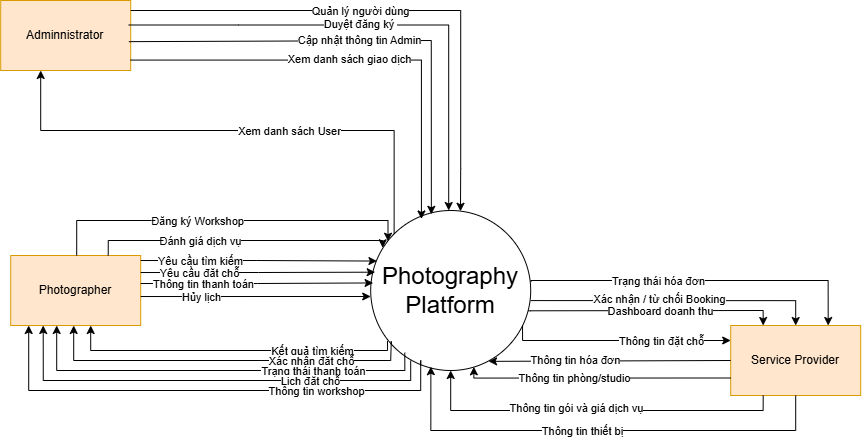
\includegraphics[width=\textwidth]{images/2.png}
	\caption{Sơ đồ ngữ cảnh của hệ thống}
	\label{fig:context-diagram}
\end{figure}


% =========================================================
% 2. YÊU CẦU NGƯỜI DÙNG
% =========================================================

\section{Yêu cầu người dùng}


\subsection{Actor}

Hệ thống gồm ba actor chính:

\begin{table}[H]sub
	\centering
	\caption{Các actor của hệ thống}
	\label{tab:actors}
	\begin{tabular}{|c|p{3.2cm}|p{8.2cm}|}
		\hline
		\textbf{\#} & \textbf{Actor} & \textbf{Mô tả} \\
		\hline
		
		1 &
		Photographer &
		Người dùng chính của hệ thống, có thể quản lý hồ sơ cá nhân, tìm kiếm
		dịch vụ, đặt chỗ, thanh toán, xem lịch sử booking và đăng ký workshop. \\
		\hline
		
		2 &
		Service Provider &
		Đơn vị cung cấp dịch vụ, có thể quản lý hồ sơ, không gian sáng tạo,
		thiết bị, gói dịch vụ, booking và workshop của mình. \\
		\hline
		
		3 &
		Administrator &
		Người quản trị hệ thống, có quyền quản lý người dùng, Service Provider,
		phê duyệt Service Provider và theo dõi giao dịch. \\
		\hline
		
	\end{tabular}
\end{table}


\subsection{Use Case}


\subsubsection{Sơ đồ Use Case}

\begin{figure}[H]
	\centering
	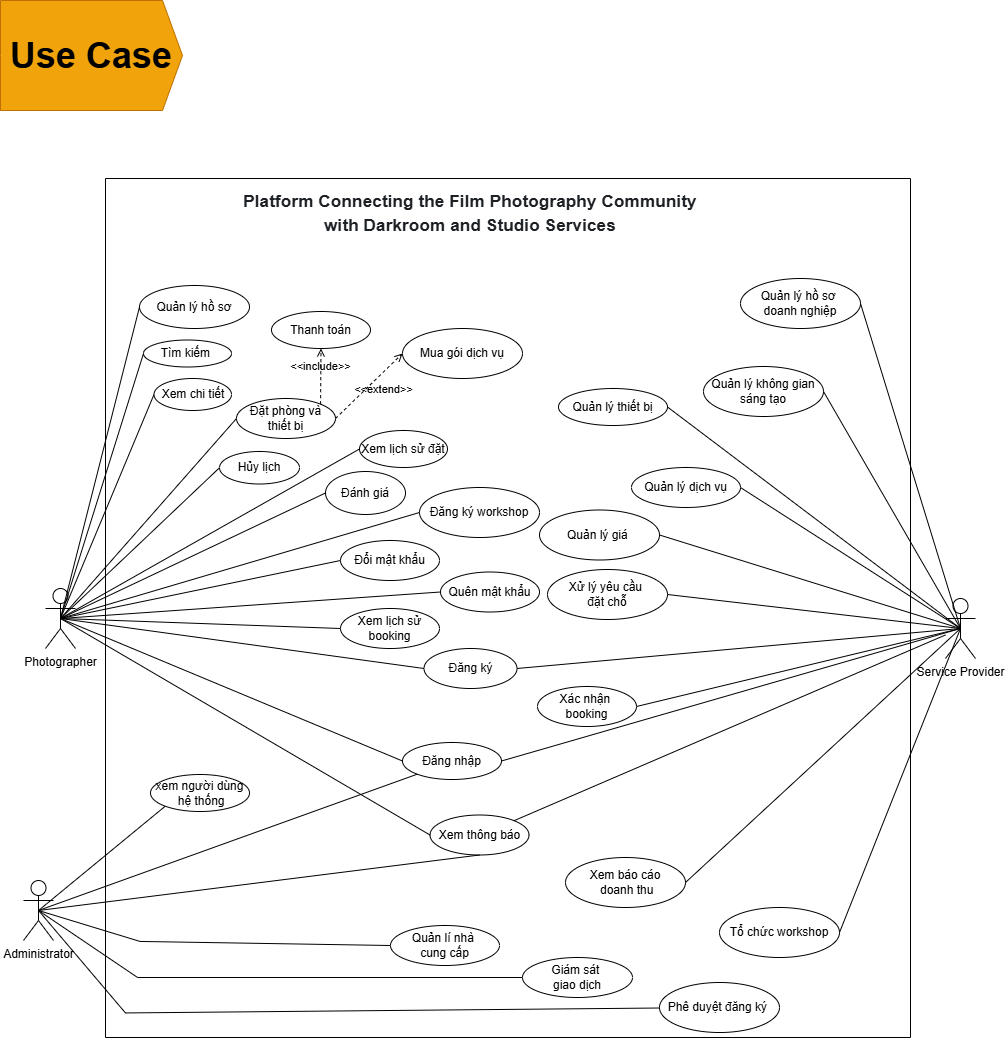
\includegraphics[width=\textwidth]{images/3.png}
	\caption{Sơ đồ Use Case của hệ thống}
	\label{fig:use-case-diagram}
\end{figure}

\newpage 

\subsubsection{Mô tả Use Case}

% =========================================================
% DANH SÁCH 34 USE CASE
% =========================================================

\setlength{\LTleft}{0pt}
\setlength{\LTright}{0pt}
\renewcommand{\arraystretch}{1.3}

\begin{longtable}{
		|>{\raggedright\arraybackslash}p{1.0cm}|
		>{\raggedright\arraybackslash}p{2.5cm}|
		>{\raggedright\arraybackslash}p{6.0cm}|
		>{\raggedright\arraybackslash}p{3.0cm}|
	}
	
	\caption{\raggedright Danh sách 34 Use Case của hệ thống}
	\label{tab:34-usecase}\\
	
	\hline
	
	\textbf{ID} &
	\textbf{Tên Use Case} &
	\textbf{Mô tả} &
	\textbf{Actor} \\
	
	\hline
	\endfirsthead
	
	\hline
	
	\textbf{ID} &
	\textbf{Tên Use Case} &
	\textbf{Mô tả} &
	\textbf{Actor} \\
	
	\hline
	\endhead
	
	UC01 &
	Đăng ký tài khoản Photographer &
	Cho phép Photographer tạo tài khoản mới. &
	Photographer \\
	
	\hline
	
	UC02 &
	Đăng nhập &
	Xác thực thông tin đăng nhập và truy cập hệ thống. &
	Photographer \\
	
	\hline
	
	UC03 &
	Đăng xuất &
	Cho phép người dùng đăng xuất khỏi hệ thống. &
	Photographer \\
	
	\hline
	
	UC04 &
	Quên mật khẩu &
	Cho phép người dùng thực hiện quy trình khôi phục mật khẩu khi quên mật khẩu. &
	Photographer \\
	
	\hline
	
	UC05 &
	Đổi mật khẩu &
	Cho phép Photographer thay đổi mật khẩu tài khoản. &
	Photographer \\
	
	\hline
	
	UC06 &
	Quản lý hồ sơ cá nhân &
	Cho phép Photographer xem và cập nhật thông tin hồ sơ cá nhân. &
	Photographer \\
	
	\hline
	
	UC07 &
	Tìm kiếm Creative Space &
	Cho phép Photographer tìm kiếm các Creative Space theo nhu cầu. &
	Photographer \\
	
	\hline
	
	UC08 &
	Xem chi tiết Creative Space &
	Hiển thị thông tin chi tiết của Creative Space được lựa chọn. &
	Photographer \\
	
	\hline
	
	UC09 &
	Đặt chỗ &
	Cho phép Photographer lựa chọn dịch vụ, thời gian và thực hiện đặt chỗ. &
	Photographer \\
	
	\hline
	
	UC10 &
	Xem chi tiết Booking &
	Hiển thị thông tin chi tiết của một Booking đã được tạo. &
	Photographer \\
	
	\hline
	
	UC11 &
	Hủy Booking &
	Cho phép Photographer hủy Booking theo trạng thái hợp lệ của Booking. &
	Photographer \\
	
	\hline
	
	UC12 &
	Xem lịch sử Booking &
	Cho phép Photographer xem danh sách các Booking đã thực hiện. &
	Photographer \\
	
	\hline
	
	UC13 &
	Xem hóa đơn &
	Cho phép Photographer xem thông tin hóa đơn liên quan đến Booking. &
	Photographer \\
	
	\hline
	
	UC14 &
	Thanh toán &
	Cho phép Photographer thực hiện thanh toán cho Booking. &
	Photographer \\
	
	\hline
	
	UC15 &
	Xem danh sách Workshop &
	Hiển thị danh sách các Workshop đang có trên hệ thống. &
	Photographer \\
	
	\hline
	
	UC16 &
	Xem chi tiết Workshop &
	Hiển thị thông tin chi tiết của Workshop được lựa chọn. &
	Photographer \\
	
	\hline
	
	UC17 &
	Đăng ký Workshop &
	Cho phép Photographer đăng ký tham gia Workshop. &
	Photographer \\
	
	\hline
	
	UC18 &
	Xem thông báo &
	Cho phép Photographer xem các thông báo liên quan đến tài khoản và hoạt động. &
	Photographer \\
	
	\hline
	
	UC19 &
	Quản lý hồ sơ Service Provider &
	Cho phép Service Provider xem và cập nhật thông tin hồ sơ của mình. &
	Service Provider \\
	
	\hline
	
	UC20 &
	Quản lý Creative Space &
	Cho phép Service Provider thêm, cập nhật và quản lý các Creative Space của mình. &
	Service Provider \\
	
	\hline
	
	UC21 &
	Quản lý Equipment &
	Cho phép Service Provider quản lý các thiết bị cung cấp cho Photographer. &
	Service Provider \\
	
	\hline
	
	UC22 &
	Quản lý Service Package &
	Cho phép Service Provider tạo và quản lý các gói dịch vụ. &
	Service Provider \\
	
	\hline
	
	UC23 &
	Quản lý Booking &
	Cho phép Service Provider xem và xử lý các Booking liên quan đến dịch vụ của mình. &
	Service Provider \\
	
	\hline
	
	UC24 &
	Xác nhận/Từ chối Booking &
	Cho phép Service Provider xác nhận hoặc từ chối Booking. &
	Service Provider \\
	
	\hline
	
	UC25 &
	Check-in/Check-out &
	Cho phép Service Provider thực hiện Check-in và Check-out cho Booking hợp lệ. &
	Service Provider \\
	
	\hline
	
	UC26 &
	Quản lý Workshop &
	Cho phép Service Provider tạo, cập nhật và quản lý Workshop. &
	Service Provider \\
	
	\hline
	
	UC27 &
	Xem danh sách người đăng ký Workshop &
	Cho phép Service Provider xem danh sách Photographer đã đăng ký Workshop. &
	Service Provider \\
	
	\hline
	
	UC28 &
	Dashboard/ Thống kê &
	Hiển thị thông tin tổng quan và các thống kê liên quan đến hoạt động của Service Provider. &
	Service Provider \\
	
	\hline
	
	UC29 &
	Quản lý thông tin thanh toán &
	Cho phép Service Provider xem và quản lý thông tin thanh toán liên quan đến dịch vụ. &
	Service Provider \\
	
	\hline
	
	UC30 &
	Xem thông báo &
	Cho phép Service Provider xem các thông báo liên quan đến hoạt động của mình. &
	Service Provider \\
	
	\hline
	
	UC31 &
	Quản lý/Xem người dùng &
	Cho phép Administrator xem và quản lý thông tin người dùng trên hệ thống. &
	Administrator \\
	
	\hline
	
	UC32 &
	Quản lý/Xem Service Provider &
	Cho phép Administrator xem và quản lý thông tin Service Provider. &
	Administrator \\
	
	\hline
	
	UC33 &
	Duyệt Service Provider &
	Cho phép Administrator xem xét và phê duyệt Service Provider trước khi cung cấp dịch vụ. &
	Administrator \\
	
	\hline
	
	UC34 &
	Xem/Quản lý giao dịch &
	Cho phép Administrator xem và quản lý các giao dịch trên hệ thống. &
	Administrator \\
	
	\hline
	
\end{longtable}

\setlength{\LTleft}{0pt}
\setlength{\LTright}{0pt}
\renewcommand{\arraystretch}{1.3}
	


% =========================================================
% 3. YÊU CẦU CHỨC NĂNG
% =========================================================

\section{Yêu cầu chức năng}


\subsection{Tổng quan chức năng hệ thống}

Hệ thống cung cấp các chức năng phục vụ Photographer, Service Provider
và Administrator.

Photographer sử dụng hệ thống để tìm kiếm dịch vụ, xem thông tin chi tiết,
đặt chỗ, thanh toán, quản lý booking và tham gia workshop.

Service Provider sử dụng hệ thống để quản lý không gian sáng tạo,
thiết bị, gói dịch vụ, booking và workshop.

Administrator thực hiện các chức năng quản trị người dùng, Service
Provider, phê duyệt đăng ký Provider và theo dõi giao dịch.


\subsubsection{Screen Flow}

Sơ đồ Screen Flow mô tả luồng di chuyển giữa các màn hình của hệ thống
theo từng nhóm người dùng. Hệ thống gồm ba Actor chính: Photographer,
Service Provider và Administrator.

\begin{figure}[H]
	\centering
	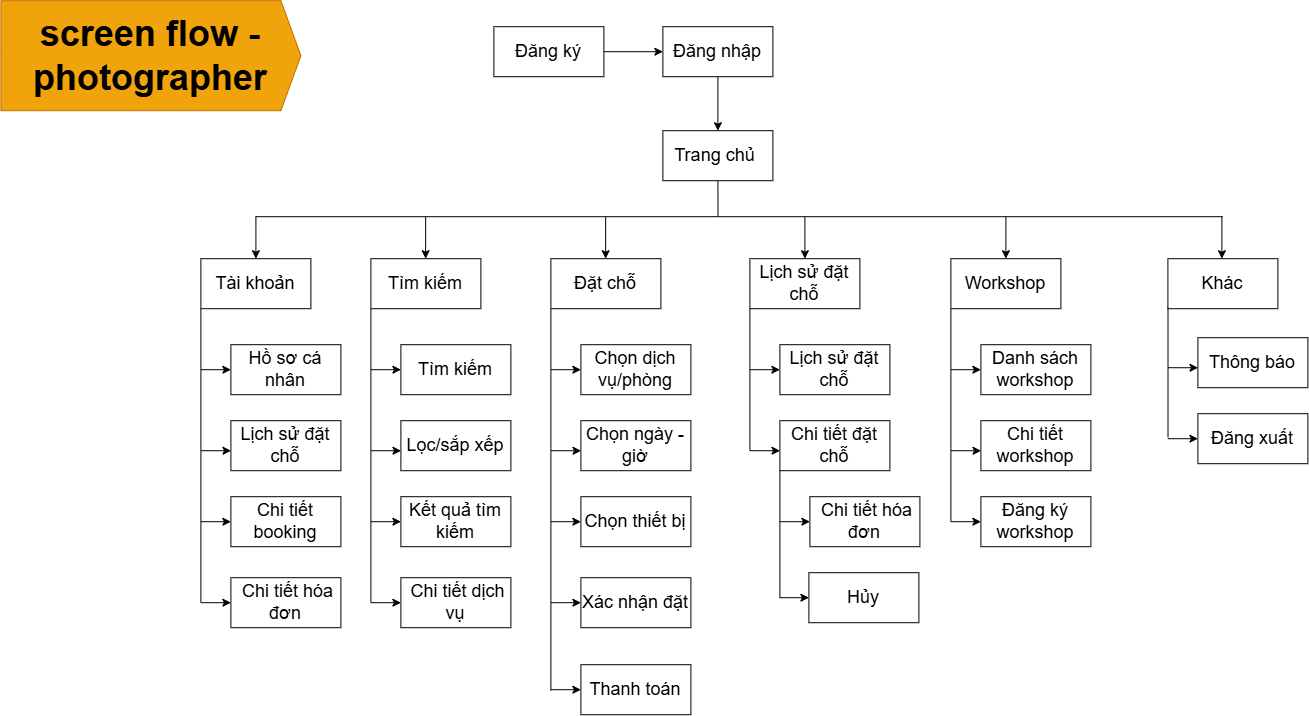
\includegraphics[width=\textwidth]{images/4.png}
	\caption{Screen Flow của Photographer}
	\label{fig:screen-flow-photographer}
\end{figure}

\begin{figure}[H]
	\centering
	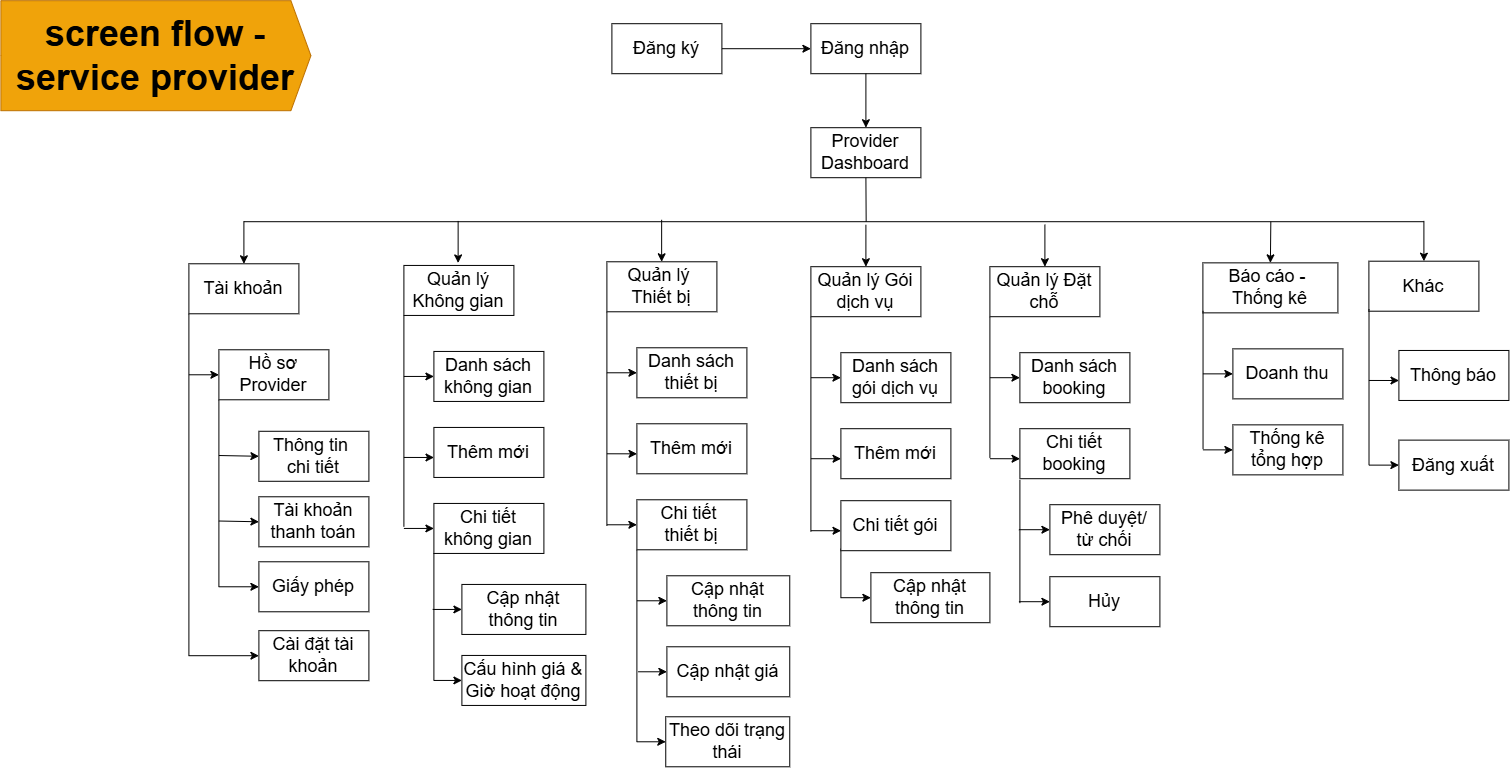
\includegraphics[width=\textwidth]{images/5.png}
	\caption{Screen Flow của Service Provider}
	\label{fig:screen-flow-provider}
\end{figure}

\begin{figure}[H]
	\centering
	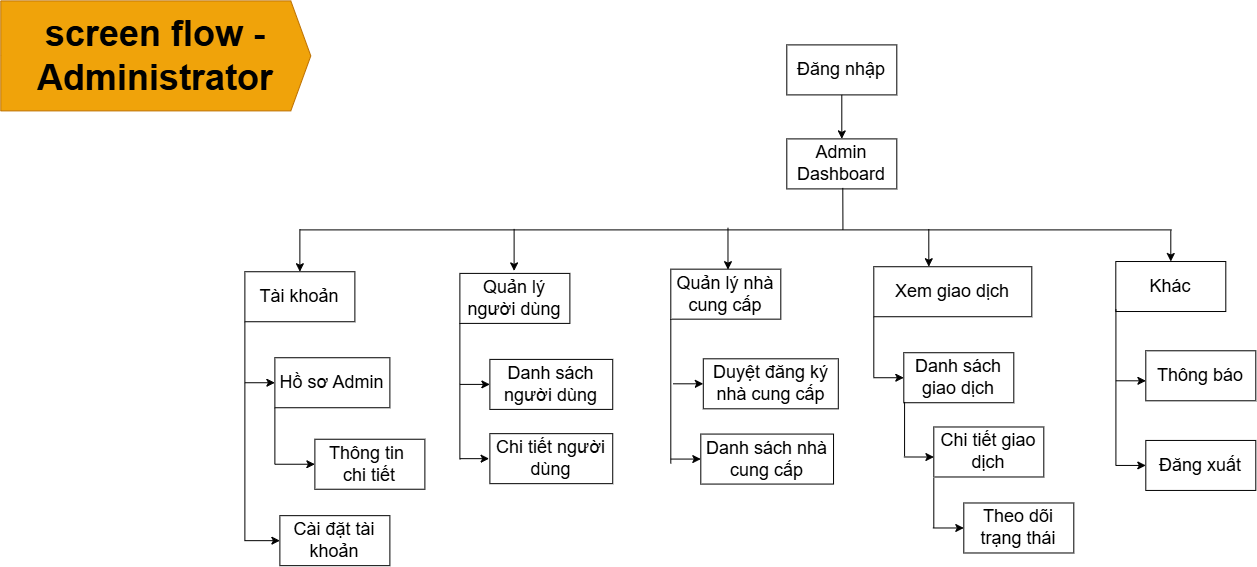
\includegraphics[width=\textwidth]{images/6.png}
	\caption{Screen Flow của Administrator}
	\label{fig:screen-flow-admin}
\end{figure}


\subsubsection{Mô tả màn hình}

\textbf{Nhóm màn hình dùng chung}

\begin{table}[H]
	\centering
	\caption{Các màn hình dùng chung}
	\label{tab:common-screens}
	\begin{tabular}{|c|p{3cm}|p{3cm}|p{5cm}|}
		\hline
		\textbf{\#} & \textbf{Nhóm} & \textbf{Màn hình} & \textbf{Mô tả} \\
		\hline
		
		1 & Xác thực & Đăng nhập &
		Cho phép người dùng đăng nhập vào hệ thống. \\
		\hline
		
		2 & Xác thực & Đăng ký &
		Cho phép Photographer và Service Provider tạo tài khoản. \\
		\hline
		
		3 & Xác thực & Đăng xuất &
		Kết thúc phiên đăng nhập hiện tại. \\
		\hline
	
	\end{tabular}
\end{table}


\textbf{Nhóm màn hình Photographer}

% =========================================================
% CÁC MÀN HÌNH PHOTOGRAPHER
% =========================================================

\setlength{\LTleft}{0pt}
\setlength{\LTright}{0pt}
\renewcommand{\arraystretch}{1.3}

\begin{longtable}{|p{0.8cm}|p{2.5cm}|p{3.2cm}|p{5.0cm}|}
	
	\caption{\raggedright Các màn hình Photographer}
	\label{tab:photographer-screens}\\
	
	\hline
	
	\textbf{\#} &
	\textbf{Nhóm} &
	\textbf{Màn hình} &
	\textbf{Mô tả} \\
	
	\hline
	\endfirsthead
	
	\hline
	
	\textbf{\#} &
	\textbf{Nhóm} &
	\textbf{Màn hình} &
	\textbf{Mô tả} \\
	
	\hline
	\endhead
	
	1 &
	Trang chủ &
	Trang chủ Photographer &
	Hiển thị tổng quan và các chức năng chính. \\
	
	\hline
	
	2 &
	Tìm kiếm &
	Tìm kiếm dịch vụ &
	Cho phép tìm kiếm Creative Space và dịch vụ. \\
	
	\hline
	
	3 &
	Tìm kiếm &
	Kết quả tìm kiếm &
	Hiển thị danh sách dịch vụ phù hợp với yêu cầu tìm kiếm. \\
	
	\hline
	
	4 &
	Tìm kiếm &
	Chi tiết dịch vụ &
	Hiển thị thông tin chi tiết của Creative Space hoặc dịch vụ. \\
	
	\hline
	
	5 &
	Booking &
	Chọn dịch vụ/không gian &
	Cho phép lựa chọn dịch vụ hoặc không gian cần đặt. \\
	
	\hline
	
	6 &
	Booking &
	Chọn ngày và giờ &
	Cho phép lựa chọn thời gian sử dụng dịch vụ. \\
	
	\hline
	
	7 &
	Booking &
	Chọn thiết bị &
	Cho phép lựa chọn thiết bị đi kèm nếu có. \\
	
	\hline
	
	8 &
	Booking &
	Xác nhận đặt chỗ &
	Hiển thị thông tin Booking trước khi xác nhận. \\
	
	\hline
	
	9 &
	Booking &
	Chi tiết Booking &
	Hiển thị thông tin chi tiết của Booking. \\
	
	\hline
	
	10 &
	Booking &
	Hủy Booking &
	Cho phép người dùng hủy Booking phù hợp. \\
	
	\hline
	
	11 &
	Booking &
	Lịch sử Booking &
	Hiển thị danh sách các Booking đã thực hiện. \\
	
	\hline
	
	12 &
	Thanh toán &
	Thanh toán &
	Hiển thị thông tin và trạng thái thanh toán. \\
	
	\hline
	
	13 &
	Hóa đơn &
	Chi tiết hóa đơn &
	Hiển thị thông tin hóa đơn của Booking. \\
	
	\hline
	
	14 &
	Workshop &
	Danh sách Workshop &
	Hiển thị danh sách Workshop. \\
	
	\hline
	
	15 &
	Workshop &
	Chi tiết Workshop &
	Hiển thị thông tin chi tiết Workshop. \\
	
	\hline
	
	16 &
	Workshop &
	Đăng ký Workshop &
	Cho phép Photographer đăng ký Workshop. \\
	
	\hline
	
	17 &
	Hồ sơ &
	Hồ sơ cá nhân &
	Cho phép Photographer xem và cập nhật thông tin cá nhân. \\
	
	\hline
	
	18 &
	Tài khoản &
	Đổi mật khẩu &
	Cho phép Photographer thay đổi mật khẩu. \\
	
	\hline
	
	19 &
	Thông báo &
	Thông báo &
	Hiển thị các thông báo của Photographer. \\
	
	\hline
	
\end{longtable}

\setlength{\LTleft}{0pt}
\setlength{\LTright}{0pt}
\renewcommand{\arraystretch}{1.3}


\textbf{Nhóm màn hình Service Provider}

\setlength{\LTleft}{0pt}
\setlength{\LTright}{0pt}
\renewcommand{\arraystretch}{1.3}

\begin{longtable}{|p{0.8cm}|p{2.5cm}|p{3.2cm}|p{5.0cm}|}
	
	\caption{\raggedright Các màn hình Service Provider}
	\label{tab:provider-screens}\\
	
	\hline
	
	\textbf{\#} &
	\textbf{Nhóm} &
	\textbf{Màn hình} &
	\textbf{Mô tả} \\
	
	\hline
	\endfirsthead
	
	\hline
	
	\textbf{\#} &
	\textbf{Nhóm} &
	\textbf{Màn hình} &
	\textbf{Mô tả} \\
	
	\hline
	\endhead
	
	1 &
	Dashboard &
	Provider Dashboard &
	Hiển thị tổng quan hoạt động của Provider. \\
	
	\hline
	
	2 &
	Hồ sơ &
	Hồ sơ Provider &
	Xem và cập nhật thông tin Provider. \\
	
	\hline
	
	3 &
	Không gian &
	Danh sách không gian &
	Hiển thị các Creative Space do Provider quản lý. \\
	
	\hline
	
	4 &
	Không gian &
	Thêm/Cập nhật không gian &
	Thêm hoặc cập nhật thông tin Creative Space. \\
	
	\hline
	
	5 &
	Thiết bị &
	Danh sách thiết bị &
	Hiển thị các thiết bị Provider quản lý. \\
	
	\hline
	
	6 &
	Thiết bị &
	Thêm/Cập nhật thiết bị &
	Thêm hoặc cập nhật thông tin thiết bị. \\
	
	\hline
	
	7 &
	Gói dịch vụ &
	Danh sách gói dịch vụ &
	Hiển thị các Service Package. \\
	
	\hline
	
	8 &
	Gói dịch vụ &
	Thêm/Cập nhật gói dịch vụ &
	Thêm hoặc cập nhật thông tin Service Package. \\
	
	\hline
	
	9 &
	Booking &
	Danh sách Booking &
	Hiển thị các Booking được gửi đến Provider. \\
	
	\hline
	
	10 &
	Booking &
	Chi tiết Booking &
	Hiển thị thông tin chi tiết Booking. \\
	
	\hline
	
	11 &
	Booking &
	Xác nhận/Từ chối &
	Cho phép Provider xử lý yêu cầu Booking. \\
	
	\hline
	
	12 &
	Booking &
	Check-in/Check-out &
	Xác nhận quá trình sử dụng dịch vụ. \\
	
	\hline
	
	13 &
	Workshop &
	Quản lý Workshop &
	Tạo và quản lý Workshop. \\
	
	\hline
	
	14 &
	Workshop &
	Người đăng ký &
	Hiển thị danh sách người đăng ký Workshop. \\
	
	\hline
	
	15 &
	Thanh toán &
	Thông tin thanh toán &
	Theo dõi thông tin thanh toán của Booking. \\
	
	\hline
	
	16 &
	Thông báo &
	Thông báo &
	Hiển thị thông báo cho Provider. \\
	
	\hline
	
\end{longtable}

\setlength{\LTleft}{0pt}
\setlength{\LTright}{0pt}
\renewcommand{\arraystretch}{1.3}


\textbf{Nhóm màn hình Administrator}

\setlength{\LTleft}{0pt}
\setlength{\LTright}{0pt}
\renewcommand{\arraystretch}{1.3}

\begin{longtable}{
		|>{\raggedright\arraybackslash}p{0.8cm}|
		>{\raggedright\arraybackslash}p{2.5cm}|
		>{\raggedright\arraybackslash}p{3.2cm}|
		>{\raggedright\arraybackslash}p{5.0cm}|
	}
	
	\caption{\raggedright Các màn hình Administrator}
	\label{tab:admin-screens}\\
	
	\hline
	
	\textbf{\#} &
	\textbf{Nhóm} &
	\textbf{Màn hình} &
	\textbf{Mô tả} \\
	
	\hline
	\endfirsthead
	
	\hline
	
	\textbf{\#} &
	\textbf{Nhóm} &
	\textbf{Màn hình} &
	\textbf{Mô tả} \\
	
	\hline
	\endhead
	
	1 &
	Dashboard &
	Admin Dashboard &
	Hiển thị tổng quan hoạt động quản trị. \\
	
	\hline
	
	2 &
	Người dùng &
	Danh sách người dùng &
	Hiển thị danh sách người dùng. \\
	
	\hline
	
	3 &
	Người dùng &
	Chi tiết người dùng &
	Hiển thị thông tin chi tiết người dùng. \\
	
	\hline
	
	4 &
	Provider &
	Danh sách Provider &
	Hiển thị danh sách Service Provider. \\
	
	\hline
	
	5 &
	Provider &
	Chi tiết Provider &
	Hiển thị thông tin chi tiết Service Provider. \\
	
	\hline
	
	6 &
	Phê duyệt &
	Danh sách đăng ký Provider &
	Hiển thị các đăng ký Service Provider cần xử lý. \\
	
	\hline
	
	7 &
	Phê duyệt &
	Phê duyệt Provider &
	Cho phép Administrator phê duyệt Service Provider. \\
	
	\hline
	
	8 &
	Giao dịch &
	Danh sách giao dịch &
	Hiển thị các giao dịch trong hệ thống. \\
	
	\hline
	
	9 &
	Giao dịch &
	Chi tiết giao dịch &
	Hiển thị thông tin chi tiết giao dịch. \\
	
	\hline
	
	10 &
	Hồ sơ &
	Hồ sơ Administrator &
	Cho phép Administrator xem và cập nhật thông tin tài khoản. \\
	
	\hline
	
	11 &
	Thông báo &
	Thông báo &
	Hiển thị các thông báo của Administrator. \\
	
	\hline
	
\end{longtable}

\setlength{\LTleft}{0pt}
\setlength{\LTright}{0pt}
\renewcommand{\arraystretch}{1.3}


\subsubsection{Phân quyền màn hình}

Hệ thống phân quyền màn hình dựa trên vai trò của người dùng. Mỗi màn hình
được giới hạn quyền truy cập tương ứng với vai trò Photographer,
Service Provider hoặc Administrator nhằm đảm bảo người dùng chỉ có thể
sử dụng các chức năng phù hợp với quyền hạn của mình.

\setlength{\LTleft}{0pt}
\setlength{\LTright}{0pt}
\renewcommand{\arraystretch}{1.3}

\begin{longtable}{|>{\raggedright\arraybackslash}p{3.0cm}|c|c|c|}
	
	\caption{\raggedright Phân quyền màn hình theo vai trò}
	\label{tab:authorization}\\
	
	\hline
	
	\textbf{Màn hình} &
	\textbf{Photographer} &
	\textbf{Service Provider} &
	\textbf{Administrator} \\
	
	\hline
	\endfirsthead
	
	\hline
	\textbf{Màn hình} &
	\textbf{Photographer} &
	\textbf{Service Provider} &
	\textbf{Administrator} \\
	\hline
	\endhead
	
	Đăng nhập &
	$\checkmark$ &
	$\checkmark$ &
	$\checkmark$ \\ \hline
	
	Đăng ký tài khoản &
	$\checkmark$ &
	$\checkmark$ &
	\\ \hline
	
	Đăng xuất &
	$\checkmark$ &
	$\checkmark$ &
	$\checkmark$ \\ \hline
	
	Trang chủ &
	$\checkmark$ &
	$\checkmark$ &
	$\checkmark$ \\ \hline
	
	Tìm kiếm dịch vụ &
	$\checkmark$ &
	&
	\\ \hline
	
	Kết quả tìm kiếm &
	$\checkmark$ &
	&
	\\ \hline
	
	Chi tiết Creative Space &
	$\checkmark$ &
	&
	\\ \hline
	
	Chọn dịch vụ/không gian Booking &
	$\checkmark$ &
	&
	\\ \hline
	
	Chọn ngày và giờ Booking &
	$\checkmark$ &
	&
	\\ \hline
	
	Chọn thiết bị &
	$\checkmark$ &
	&
	\\ \hline
	
	Xác nhận Booking &
	$\checkmark$ &
	&
	\\ \hline
	
	Chi tiết Booking &
	$\checkmark$ &
	$\checkmark$ &
	\\ \hline
	
	Hủy Booking &
	$\checkmark$ &
	&
	\\ \hline
	
	Lịch sử Booking &
	$\checkmark$ &
	&
	\\ \hline
	
	Thanh toán &
	$\checkmark$ &
	$\checkmark$ &
	$\checkmark$ \\ \hline
	
	Chi tiết hóa đơn &
	$\checkmark$ &
	&
	\\ \hline
	
	Danh sách Workshop &
	$\checkmark$ &
	$\checkmark$ &
	\\ \hline
	
	Chi tiết Workshop &
	$\checkmark$ &
	$\checkmark$ &
	\\ \hline
	
	Đăng ký Workshop &
	$\checkmark$ &
	&
	\\ \hline
	
	Hồ sơ Photographer &
	$\checkmark$ &
	&
	\\ \hline
	
	Hồ sơ Service Provider &
	&
	$\checkmark$ &
	\\ \hline
	
	Đổi mật khẩu &
	$\checkmark$ &
	$\checkmark$ &
	$\checkmark$ \\ \hline
	
	Thông báo Photographer &
	$\checkmark$ &
	&
	\\ \hline
	
	Thông báo Service Provider &
	&
	$\checkmark$ &
	\\ \hline
	
	Thông báo Administrator &
	&
	&
	$\checkmark$ \\ \hline
	
	Provider Dashboard &
	&
	$\checkmark$ &
	\\ \hline
	
	Quản lý Creative Space &
	&
	$\checkmark$ &
	\\ \hline
	
	Quản lý thiết bị &
	&
	$\checkmark$ &
	\\ \hline
	
	Quản lý gói dịch vụ &
	&
	$\checkmark$ &
	\\ \hline
	
	Quản lý Booking &
	&
	$\checkmark$ &
	\\ \hline
	
	Xác nhận/Từ chối Booking &
	&
	$\checkmark$ &
	\\ \hline
	
	Check-in/Check-out &
	&
	$\checkmark$ &
	\\ \hline
	
	Quản lý Workshop &
	&
	$\checkmark$ &
	\\ \hline
	
	Người đăng ký Workshop &
	&
	$\checkmark$ &
	\\ \hline
	
	Thông tin thanh toán Provider &
	&
	$\checkmark$ &
	\\ \hline
	
	Quản lý người dùng &
	&
	&
	$\checkmark$ \\ \hline
	
	Quản lý Provider &
	&
	&
	$\checkmark$ \\ \hline
	
	Phê duyệt Provider &
	&
	&
	$\checkmark$ \\ \hline
	
	Quản lý giao dịch &
	&
	&
	$\checkmark$ \\ \hline
	
\end{longtable}

\setlength{\LTleft}{0pt}
\setlength{\LTright}{0pt}
\renewcommand{\arraystretch}{1.3}


\subsubsection{Chức năng không thông qua màn hình}

Một số chức năng của hệ thống được thực hiện tự động ở phía Backend mà
không yêu cầu người dùng thao tác trực tiếp trên một màn hình riêng biệt.
Các chức năng này hỗ trợ xác thực, xử lý thông tin đặt chỗ, thanh toán,
quản lý trạng thái và gửi thông báo trong quá trình vận hành hệ thống.
Bảng dưới đây tổng hợp các chức năng không thông qua màn hình được triển
khai trong hệ thống.

\setlength{\LTleft}{0pt}
\setlength{\LTright}{0pt}
\renewcommand{\arraystretch}{1.3}

\begin{longtable}{
		|>{\raggedright\arraybackslash}p{0.8cm}|
		>{\raggedright\arraybackslash}p{3.0cm}|
		>{\raggedright\arraybackslash}p{3.0cm}|
		>{\raggedright\arraybackslash}p{4.7cm}|
	}
	
	\caption{\raggedright Các chức năng không thông qua màn hình}
	\label{tab:non-screen}\\
	
	\hline
	
	\textbf{\#} &
	\textbf{Chức năng} &
	\textbf{Module} &
	\textbf{Mô tả} \\
	
	\hline
	\endfirsthead
	
	\hline
	
	\textbf{\#} &
	\textbf{Chức năng} &
	\textbf{Module} &
	\textbf{Mô tả} \\
	
	\hline
	\endhead
	
	1 &
	Xác thực tài khoản &
	Authentication &
	Xử lý xác thực thông tin tài khoản và trạng thái tài khoản trong quá trình đăng nhập và truy cập các chức năng yêu cầu xác thực. \\
	
	\hline
	
	2 &
	Xác thực OTP &
	Authentication &
	Xử lý mã OTP phục vụ các chức năng xác thực tài khoản, đặc biệt trong quá trình quên mật khẩu và đặt lại mật khẩu. \\
	
	\hline
	
	3 &
	Kiểm tra quyền truy cập &
	Authorization &
	Kiểm tra vai trò của người dùng và xác định quyền thực hiện các chức năng tương ứng trong hệ thống. \\
	
	\hline
	
	4 &
	Kiểm tra khả dụng Booking &
	Booking &
	Kiểm tra thông tin Creative Space, thiết bị và thời gian được lựa chọn trước khi xử lý yêu cầu Booking. \\
	
	\hline
	
	5 &
	Tính tổng chi phí Booking &
	Booking &
	Tự động tính toán tổng chi phí dựa trên các dịch vụ, Creative Space và thiết bị được lựa chọn trong Booking. \\
	
	\hline
	
	6 &
	Cập nhật trạng thái Booking &
	Booking &
	Tự động cập nhật trạng thái Booking theo quá trình xử lý như xác nhận, từ chối, hủy, check-in và check-out. \\
	
	\hline
	
	7 &
	Xử lý thanh toán &
	Payment &
	Xử lý thông tin thanh toán và cập nhật trạng thái thanh toán tương ứng với Booking. \\
	
	\hline
	
	8 &
	Tạo hóa đơn &
	Invoice &
	Tạo thông tin hóa đơn tương ứng với Booking và lưu trữ thông tin hóa đơn trong hệ thống. \\
	
	\hline
	
	9 &
	Kiểm tra trạng thái Provider &
	Service Provider &
	Kiểm tra trạng thái phê duyệt của Service Provider để xác định Provider có đủ điều kiện cung cấp dịch vụ trên hệ thống hay không. \\
	
	\hline
	
	10 &
	Xử lý đăng ký Workshop &
	Workshop &
	Xử lý thông tin đăng ký Workshop và cập nhật thông tin đăng ký của Photographer trong hệ thống. \\
	
	\hline
	
	11 &
	Gửi thông báo &
	Notification &
	Tạo và gửi thông báo đến người dùng liên quan khi phát sinh các sự kiện trong quá trình sử dụng hệ thống. \\
	
	\hline
	
\end{longtable}

\setlength{\LTleft}{0pt}
\setlength{\LTright}{0pt}
\renewcommand{\arraystretch}{1.3}


\subsubsection{Sơ đồ quan hệ thực thể}

Sơ đồ quan hệ thực thể mô tả các thực thể chính trong hệ thống và mối
quan hệ giữa các thực thể.

\begin{figure}[H]
	\centering
	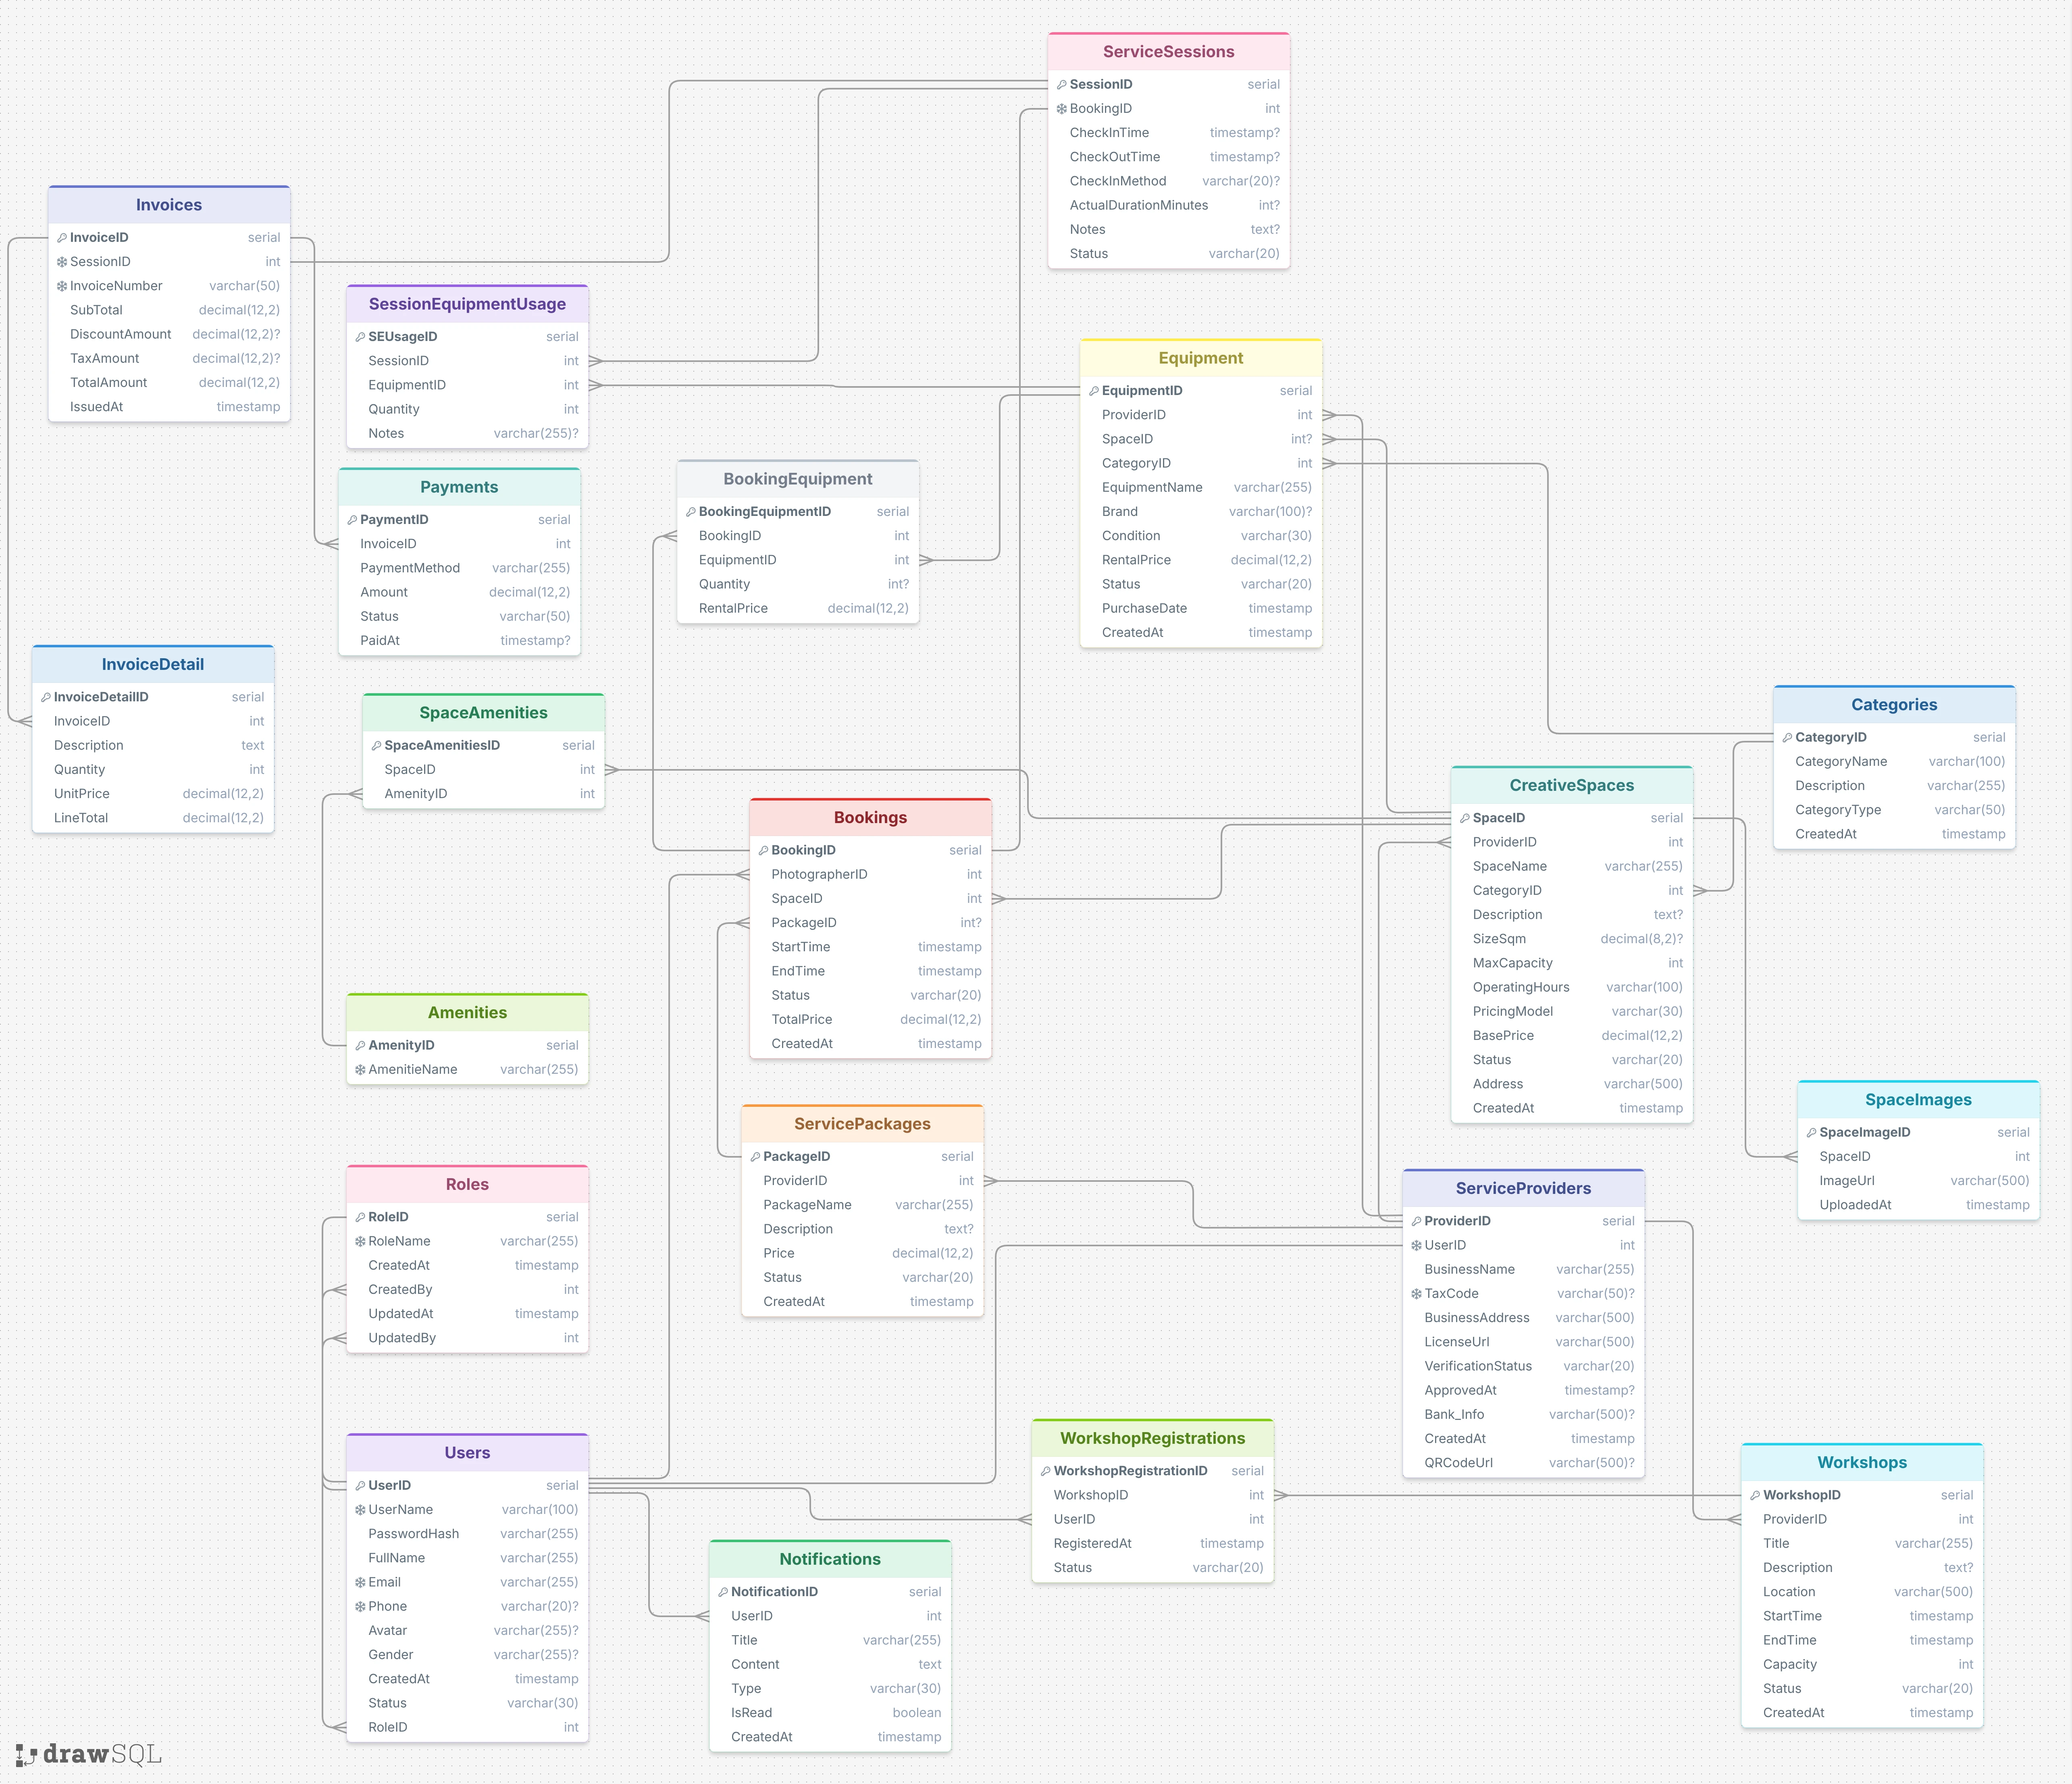
\includegraphics[width=\textwidth]{images/7.png}
	\caption{Sơ đồ quan hệ thực thể của hệ thống}
	\label{fig:erd}
\end{figure}


% =========================================================
% 3.2 XÁC THỰC
% =========================================================

\subsection{Xác thực}

Chức năng xác thực chịu trách nhiệm xác thực người dùng trước khi cho
phép truy cập vào hệ thống.

\subsubsection{Đăng nhập}

Người dùng nhập thông tin tài khoản để đăng nhập.

Hệ thống kiểm tra thông tin đăng nhập và trạng thái tài khoản. Nếu thông
tin hợp lệ, hệ thống chuyển người dùng đến Dashboard tương ứng với vai
trò. Nếu thông tin không hợp lệ, hệ thống hiển thị thông báo lỗi.

\subsubsection{Đăng ký}

Photographer và Service Provider có thể đăng ký tài khoản mới trên hệ
thống.

Sau khi đăng ký thành công, thông tin tài khoản được lưu vào hệ thống.

\subsubsection{Đăng xuất}

Người dùng có thể đăng xuất để kết thúc phiên làm việc hiện tại.


% =========================================================
% 3.3 QUẢN LÝ PHOTOGRAPHER
% =========================================================

\subsection{Quản lý Photographer}

Chức năng quản lý Photographer cho phép người dùng quản lý thông tin
tài khoản và hồ sơ cá nhân.

\subsubsection{Quản lý hồ sơ Photographer}

Photographer có thể xem và cập nhật thông tin cá nhân của mình.

Thông tin được cập nhật sẽ được lưu lại để sử dụng trong các chức năng
khác của hệ thống.

\subsubsection{Quên mật khẩu}

Photographer có thể yêu cầu khôi phục mật khẩu khi không nhớ mật khẩu
đăng nhập.

Hệ thống thực hiện quy trình xác thực cần thiết và cho phép người dùng
thiết lập mật khẩu mới.

\subsubsection{Đổi mật khẩu}

Photographer đã đăng nhập có thể thay đổi mật khẩu tài khoản.


% =========================================================
% 3.4 TÌM KIẾM VÀ KHÁM PHÁ DỊCH VỤ
% =========================================================

\subsection{Tìm kiếm và khám phá dịch vụ}

Chức năng này hỗ trợ Photographer tìm kiếm và khám phá các dịch vụ
phòng tối, studio và các tài nguyên được cung cấp trên nền tảng.

\subsubsection{Tìm kiếm dịch vụ}

Photographer nhập thông tin tìm kiếm để tìm các creative space hoặc
dịch vụ phù hợp.

Hệ thống trả về danh sách các kết quả phù hợp với thông tin tìm kiếm.

\subsubsection{Lọc và sắp xếp dịch vụ}

Photographer có thể lọc và sắp xếp danh sách kết quả dựa trên các tiêu
chí được hệ thống hỗ trợ.

\subsubsection{Xem chi tiết dịch vụ}

Photographer có thể chọn một dịch vụ trong danh sách để xem thông tin
chi tiết trước khi thực hiện booking.


% =========================================================
% 3.5 QUẢN LÝ ĐẶT CHỖ
% =========================================================

\subsection{Quản lý đặt chỗ}

Chức năng quản lý đặt chỗ hỗ trợ Photographer thực hiện quá trình lựa
chọn dịch vụ và tạo booking.

\subsubsection{Chọn dịch vụ/không gian}

Photographer lựa chọn creative space hoặc dịch vụ cần sử dụng.

\subsubsection{Chọn ngày và giờ}

Photographer lựa chọn ngày và khoảng thời gian sử dụng dịch vụ.

Hệ thống kiểm tra khả dụng của khoảng thời gian được lựa chọn.

\subsubsection{Chọn thiết bị}

Photographer có thể lựa chọn thiết bị đi kèm nếu dịch vụ hỗ trợ.

\subsubsection{Xác nhận booking}

Hệ thống hiển thị thông tin dịch vụ, thời gian, thiết bị và chi phí để
Photographer kiểm tra trước khi xác nhận booking.

\subsubsection{Hủy booking}

Photographer có thể hủy booking phù hợp với trạng thái hiện tại của
booking.

\subsubsection{Check-in/Check-out}

Hệ thống hỗ trợ ghi nhận trạng thái bắt đầu và kết thúc sử dụng dịch vụ
thông qua chức năng check-in và check-out.


% =========================================================
% 3.6 THANH TOÁN VÀ QUẢN LÝ BOOKING
% =========================================================

\subsection{Thanh toán và quản lý booking}

Chức năng này hỗ trợ Photographer theo dõi booking và thực hiện các
nghiệp vụ liên quan đến thanh toán.

\subsubsection{Thanh toán}

Photographer thực hiện thanh toán cho booking thông qua phương thức thanh
toán được hệ thống hỗ trợ.

Sau khi thanh toán được xử lý, hệ thống cập nhật trạng thái thanh toán
và booking.

\subsubsection{Xem lịch sử booking}

Photographer có thể xem danh sách các booking đã thực hiện.

Lịch sử booking giúp người dùng theo dõi các lần đặt chỗ trước đó.

\subsubsection{Xem chi tiết booking}

Photographer có thể xem thông tin chi tiết của từng booking bao gồm
dịch vụ, thời gian, chi phí và trạng thái booking.

\subsubsection{Xem hóa đơn}

Photographer có thể xem thông tin hóa đơn tương ứng với booking.


% =========================================================
% 3.7 QUẢN LÝ WORKSHOP
% =========================================================

\subsection{Quản lý Workshop}

Chức năng Workshop hỗ trợ Photographer xem và đăng ký các workshop được
tổ chức trên nền tảng.

\subsubsection{Xem danh sách Workshop}

Photographer có thể truy cập danh sách các workshop đang được tổ chức
trên hệ thống.

Danh sách workshop hiển thị các thông tin cơ bản giúp người dùng lựa
chọn workshop phù hợp.

\subsubsection{Xem chi tiết Workshop}

Photographer có thể chọn một workshop để xem thông tin chi tiết.

Thông tin chi tiết bao gồm các thông tin được Provider cung cấp như tên
workshop, nội dung, thời gian và các thông tin liên quan.

\subsubsection{Đăng ký Workshop}

Photographer có thể đăng ký tham gia workshop.

Hệ thống kiểm tra thông tin đăng ký và lưu thông tin tham gia workshop
của Photographer.


% =========================================================
% 3.8 QUẢN LÝ SERVICE PROVIDER
% =========================================================

\subsection{Quản lý Service Provider}

Chức năng quản lý Service Provider hỗ trợ Provider quản lý các hoạt động
cung cấp dịch vụ trên nền tảng.

\subsubsection{Quản lý không gian}

Service Provider có thể thêm, cập nhật và quản lý thông tin các creative
space thuộc quyền quản lý của mình.

\subsubsection{Quản lý thiết bị}

Service Provider có thể thêm, cập nhật và quản lý các thiết bị được cung
cấp trên nền tảng.

\subsubsection{Quản lý gói dịch vụ}

Service Provider có thể tạo và cập nhật các service package.

Thông tin gói dịch vụ được sử dụng khi Photographer tìm kiếm và đặt
dịch vụ.

\subsubsection{Quản lý booking}

Service Provider có thể xem danh sách booking được gửi đến mình.

Provider có thể xem thông tin chi tiết của từng booking để xử lý.

\subsubsection{Xác nhận hoặc từ chối booking}

Service Provider có thể xác nhận hoặc từ chối yêu cầu booking từ
Photographer.

Sau khi xử lý, trạng thái booking được cập nhật trong hệ thống.

\subsubsection{Check-in/Check-out}

Service Provider có thể thực hiện hoặc ghi nhận trạng thái check-in và
check-out của booking.

Chức năng này giúp xác định quá trình sử dụng dịch vụ của Photographer.

\subsubsection{Quản lý Workshop}

Service Provider có thể tạo và quản lý các workshop do mình tổ chức.

Provider có thể cập nhật thông tin workshop để Photographer xem và đăng
ký tham gia.

\subsubsection{Xem người đăng ký Workshop}

Service Provider có thể xem danh sách Photographer đã đăng ký tham gia
một workshop.

Thông tin này giúp Provider theo dõi số lượng người tham gia.

\subsubsection{Quản lý hồ sơ Provider}

Service Provider có thể xem và cập nhật thông tin hồ sơ của mình.

\subsubsection{Xem Dashboard}

Service Provider có thể xem Dashboard để theo dõi tổng quan hoạt động
của mình trên hệ thống.

\subsubsection{Quản lý thông tin thanh toán}

Service Provider có thể xem thông tin thanh toán liên quan đến các
booking được thực hiện trên nền tảng.


% =========================================================
% 3.9 QUẢN LÝ ADMINISTRATOR
% =========================================================

\subsection{Quản lý Administrator}

Administrator chịu trách nhiệm quản lý các thông tin và hoạt động quản
trị chính của hệ thống.

\subsubsection{Quản lý người dùng}

Administrator có thể xem danh sách và thông tin người dùng trên hệ thống.

\subsubsection{Quản lý Service Provider}

Administrator có thể xem và quản lý thông tin các Service Provider.

\subsubsection{Phê duyệt Service Provider}

Administrator có thể xem các đăng ký Service Provider và thực hiện phê
duyệt.

Chỉ Service Provider được phê duyệt mới có thể thực hiện các hoạt động
cung cấp dịch vụ theo quy định của hệ thống.

\subsubsection{Quản lý giao dịch}

Administrator có thể xem danh sách và thông tin các giao dịch trên hệ
thống để theo dõi hoạt động thanh toán.


% =========================================================
% 3.10 QUẢN LÝ THÔNG BÁO
% =========================================================

\subsection{Quản lý thông báo}

Hệ thống cung cấp chức năng thông báo cho Photographer, Service Provider
và Administrator.

\subsubsection{Xem thông báo}

Người dùng có thể xem danh sách các thông báo liên quan đến hoạt động
của tài khoản.

Thông báo có thể liên quan đến booking, thanh toán, phê duyệt Provider
hoặc các thay đổi trạng thái khác trong hệ thống.


% =========================================================
% 4. YÊU CẦU PHI CHỨC NĂNG
% =========================================================

\section{Yêu cầu phi chức năng}


\subsection{Giao diện bên ngoài}

Hệ thống cung cấp các giao diện bên ngoài phục vụ người dùng và các
hoạt động nghiệp vụ chính.

\begin{itemize}
	\item \textbf{Giao diện người dùng:} cung cấp giao diện web cho ba
	nhóm người dùng gồm Photographer, Service Provider và Administrator.
	
	\item \textbf{Giao diện thanh toán:} cung cấp giao diện để
	Photographer thực hiện thanh toán cho Booking thông qua
	QR/chuyển khoản ngân hàng và theo dõi trạng thái thanh toán.
	
	\item \textbf{Giao diện thông báo:} cung cấp giao diện hiển thị
	các thông báo liên quan đến hoạt động của hệ thống cho
	Photographer, Service Provider và Administrator.
\end{itemize}


\subsection{Thuộc tính chất lượng}

\begin{itemize}
	
	\item \textbf{Bảo mật:} hệ thống phải xác thực người dùng và
	kiểm soát quyền truy cập dựa trên vai trò Photographer,
	Service Provider và Administrator.
	
	\item \textbf{Tính toàn vẹn dữ liệu:} hệ thống phải đảm bảo
	dữ liệu người dùng, Creative Space, Equipment, Service Package,
	Booking, Workshop, thanh toán và hóa đơn được lưu trữ chính xác
	và nhất quán.
	
	\item \textbf{Tính khả dụng:} hệ thống phải cho phép người dùng
	truy cập và sử dụng các chức năng tương ứng với quyền được cấp.
	
	\item \textbf{Khả năng mở rộng:} hệ thống nên có khả năng mở rộng
	để đáp ứng sự gia tăng về số lượng người dùng, Creative Space,
	dịch vụ, Workshop và Booking.
	
	\item \textbf{Khả năng bảo trì:} hệ thống được tổ chức thành các
	module chức năng và các thành phần riêng biệt, giúp thuận tiện
	cho việc bảo trì, sửa lỗi và phát triển thêm chức năng.
	
\end{itemize}


% =========================================================
% 5. PHỤ LỤC YÊU CẦU
% =========================================================
\section{Phụ lục yêu cầu}
\subsection{Quy tắc nghiệp vụ}

\begin{table}[H]
	\centering
	\caption{Các quy tắc nghiệp vụ}
	\label{tab:business-rules}
	\begin{tabular}{|c|p{11cm}|}
		\hline
		\textbf{ID} & \textbf{Quy tắc nghiệp vụ} \\
		\hline
		
		BR-01 &
		Mỗi Photographer chỉ được tạo một tài khoản trên hệ thống. \\
		\hline
		
		BR-02 &
		Service Provider phải được Administrator phê duyệt trước khi
		cung cấp dịch vụ trên nền tảng. \\
		\hline
		
		BR-03 &
		Photographer chỉ có thể đặt Creative Space và các tài nguyên
		đang ở trạng thái khả dụng. \\
		\hline
		
		BR-04 &
		Một Creative Space hoặc Equipment không được phép có các
		booking bị trùng thời gian. \\
		\hline
		
		BR-05 &
		Photographer phải thực hiện thanh toán cho booking theo
		thông tin và trạng thái thanh toán được hệ thống cung cấp. \\
		\hline
		
		BR-06 &
		Service Provider chỉ được quản lý Creative Space, Equipment,
		Service Package, Workshop và Booking thuộc phạm vi của mình. \\
		\hline
		
		BR-07 &
		Chỉ Administrator mới có quyền phê duyệt Service Provider. \\
		\hline
		
		BR-08 &
		Chỉ người dùng đã xác thực mới được truy cập các chức năng
		yêu cầu đăng nhập. \\
		\hline
		
		BR-09 &
		Booking phải được xử lý theo các trạng thái tương ứng trong
		quy trình đặt chỗ và sử dụng dịch vụ. \\
		\hline
		
		BR-10 &
		Check-in và check-out chỉ được thực hiện đối với một Booking
		hợp lệ và có phiên dịch vụ tương ứng. \\
		\hline
		
		BR-11 &
		Một Photographer không được đăng ký trùng một Workshop
		nhiều lần. \\
		\hline
		
		BR-12 &
		Thông báo phải được tạo và hiển thị đến đúng người dùng
		liên quan đến hoạt động của hệ thống. \\
		\hline
		
	\end{tabular}
\end{table}

\subsection{Yêu cầu hệ thống}

\subsubsection{Xác thực và phân quyền}

Hệ thống phải triển khai cơ chế phân quyền dựa trên vai trò (Role-Based
Access Control - RBAC). Người dùng chỉ được phép truy cập các chức năng
phù hợp với vai trò được phân công, bao gồm Photographer, Service Provider
và Administrator.

\subsubsection{Bảo mật dữ liệu}

Thông tin tài khoản, hồ sơ người dùng, thông tin Booking, thanh toán,
hóa đơn và các dữ liệu nghiệp vụ khác phải được bảo vệ thông qua cơ chế
xác thực và kiểm soát quyền truy cập phù hợp.

\subsubsection{Khả năng mở rộng}

Hệ thống phải có khả năng đáp ứng sự gia tăng về số lượng người dùng,
Creative Space, Equipment, Service Package, Workshop và Booking mà không
làm suy giảm đáng kể hiệu năng của hệ thống.

\subsubsection{Tính khả dụng}

Hệ thống cần duy trì khả năng truy cập và sử dụng các chức năng cho
Photographer, Service Provider và Administrator trong thời gian hoạt động
bình thường, ngoại trừ thời gian bảo trì hoặc khi xảy ra sự cố hệ thống.

\subsubsection{Khả năng bảo trì}

Các module của hệ thống phải được tổ chức tương đối độc lập nhằm thuận
tiện cho việc bảo trì, sửa lỗi và phát triển thêm các chức năng trong
tương lai.
	
	% ============================================================
	% CHAPTER IV
	% DESIGN
	% ============================================================
	
	\chapter{MÔ TẢ THIẾT KẾ PHẦN MỀM}

\section{Thiết kế hệ thống}
\subsection{Kiến trúc hệ thống}
Kiến trúc hệ thống được thiết kế theo mô hình phân lớp, bao gồm các
thành phần chính: giao diện người dùng, máy chủ xử lý
nghiệp vụ và cơ sở dữ liệu. Các thành phần phối
hợp với nhau thông qua các API để tiếp nhận yêu cầu, xử lý nghiệp vụ
và trao đổi dữ liệu.

\begin{figure}[H]
	\centering
	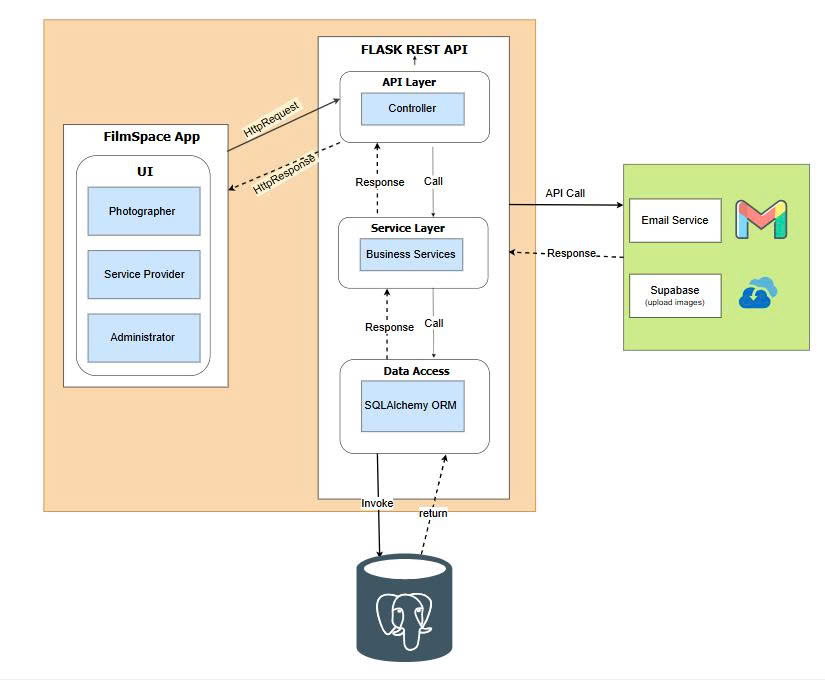
\includegraphics[width=\textwidth]{images/5.jpg}
	\caption{Kiến trúc tổng thể của hệ thống}
	\label{fig:system-arcFronthitecture}
\end{figure}

\subsubsection{Frontend}

Frontend của hệ thống được xây dựng dưới dạng ứng dụng Web, sử dụng
HTML, CSS và JavaScript để xây dựng giao diện và xử lý tương tác với người dùng.

\begin{itemize}
	\item \textbf{HTML:} Xây dựng cấu trúc các trang Web dành cho
	Photographer, Service Provider và Administrator.
	
	\item \textbf{CSS:} Thiết kế giao diện và bố cục cho các trang,
	bao gồm các thành phần dùng chung và giao diện theo từng nhóm người dùng.
	
	\item \textbf{JavaScript:} Xử lý tương tác, kiểm tra dữ liệu đầu vào
	và cập nhật nội dung động trên giao diện.
	
	\item \textbf{Fetch API:} Gửi request từ Frontend đến các REST API
	của Backend để thực hiện xác thực, quản lý hồ sơ, tìm kiếm,
	Booking, Workshop, thanh toán và các chức năng quản trị.
\end{itemize}

\begin{figure}[H]
	\centering
	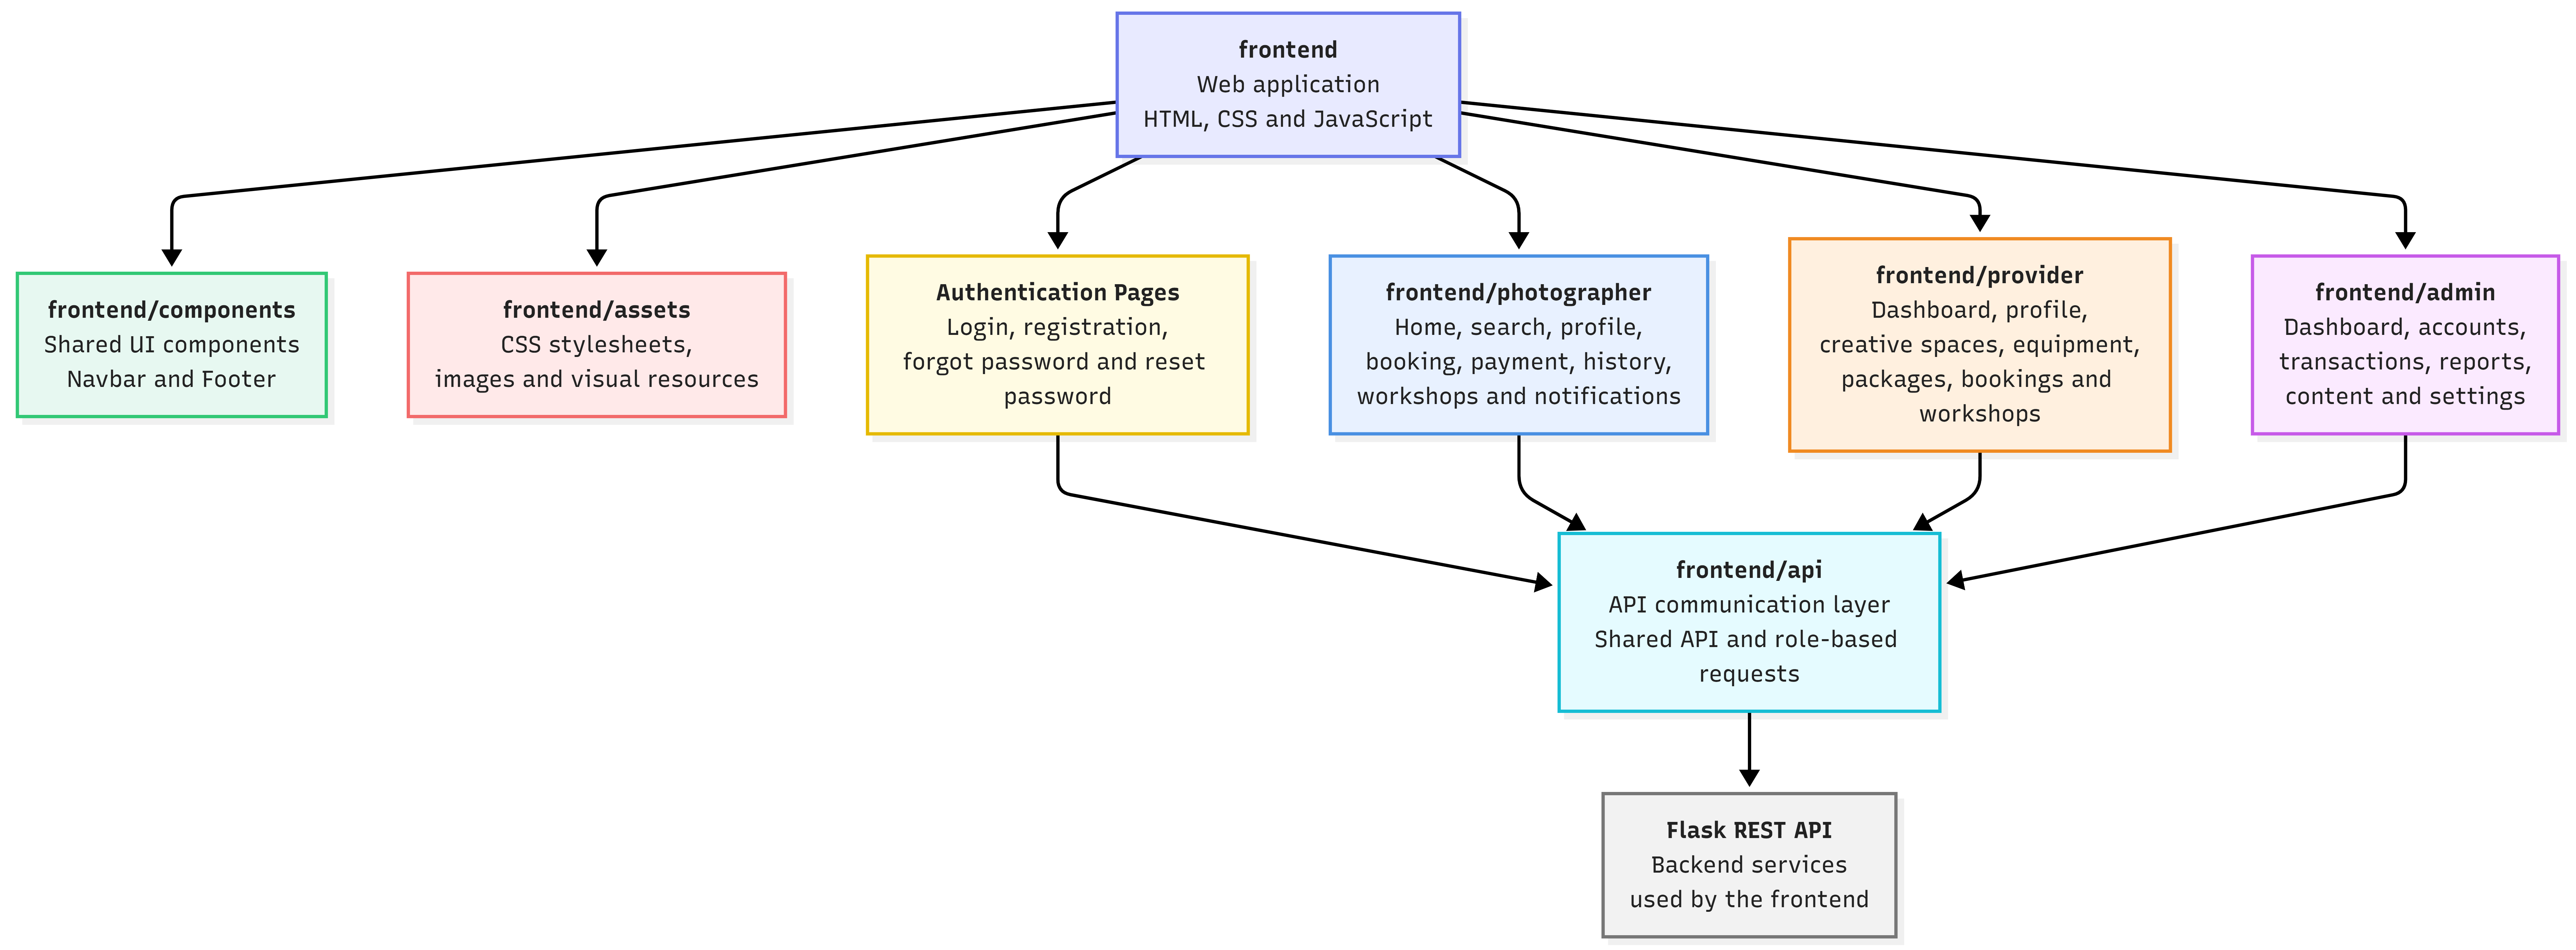
\includegraphics[width=\textwidth]{images/8.png}
	\caption{Kiến trúc Frontend}
	\label{fig:frontend-architecture}
\end{figure}


\subsubsection{Backend}

Backend của hệ thống được xây dựng bằng Flask theo kiến trúc
Clean Architecture, cung cấp các REST API và xử lý nghiệp vụ của hệ thống.

\begin{itemize}
	\item \textbf{Flask:} Framework chính để xây dựng Backend và cung cấp
	các REST API cho Frontend.
	
	\item \textbf{Clean Architecture:} Tổ chức Backend thành các lớp
	API, Services, Domain và Infrastructure, giúp phân tách trách nhiệm
	và hỗ trợ bảo trì hệ thống.
	
	
	\item \textbf{PostgreSQL:} Hệ quản trị cơ sở dữ liệu quan hệ,
	lưu trữ thông tin người dùng, Service Provider, Creative Space,
	Equipment, Booking, Workshop, Invoice, Payment và Notification.
	
	
	\item \textbf{Email Service:} Hỗ trợ gửi mã OTP phục vụ chức năng
	quên mật khẩu và đặt lại mật khẩu.
\end{itemize}

\begin{figure}[H]
	\centering
	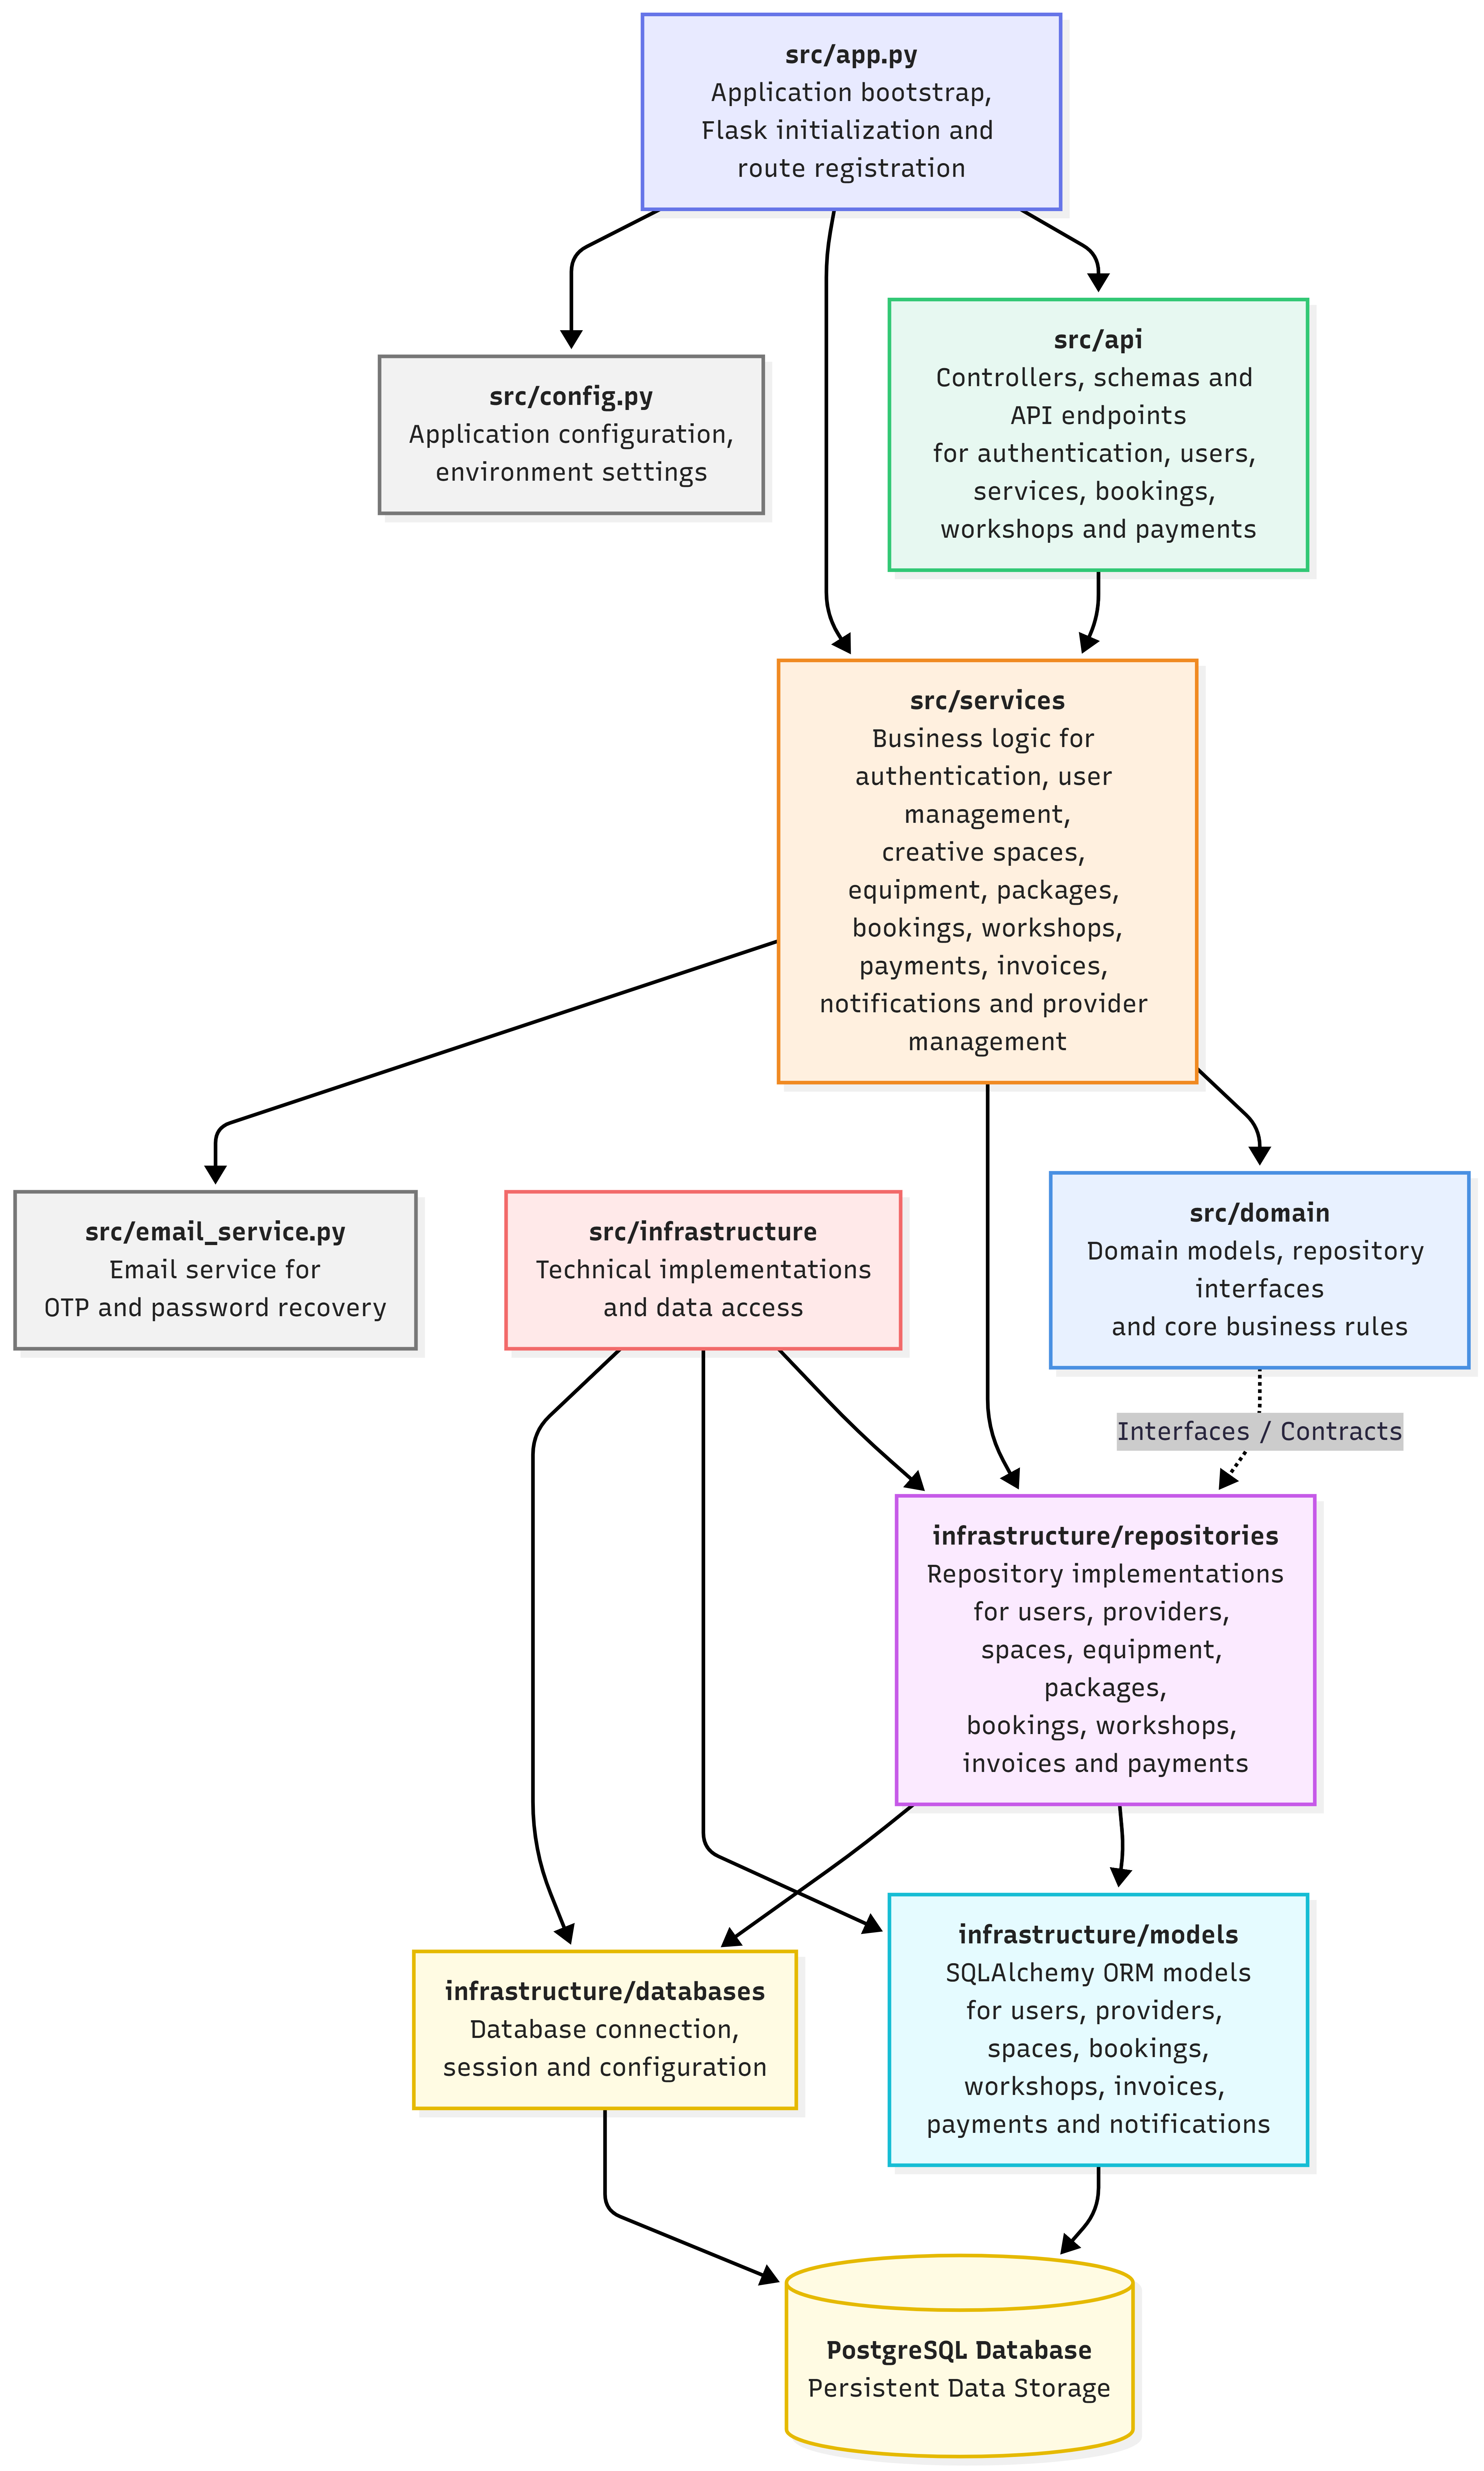
\includegraphics[width=\textwidth]{images/9.png}
	\caption{Kiến trúc Backend}
	\label{fig:backend-architecture}
\end{figure}

\subsubsection{Third-party}

\begin{itemize}
	\item \textbf{GitHub:} Nền tảng quản lý mã nguồn, được sử dụng để
	lưu trữ source code và hỗ trợ quản lý phiên bản trong quá trình
	phát triển hệ thống.
	
	\item \textbf{Supabase:} Nền tảng cung cấp dịch vụ PostgreSQL,
	được sử dụng để lưu trữ và quản lý dữ liệu của hệ thống.
\end{itemize}
\subsection{Package Diagram}
\subsubsection{Frontend}

\begin{figure}[H]
	\centering
	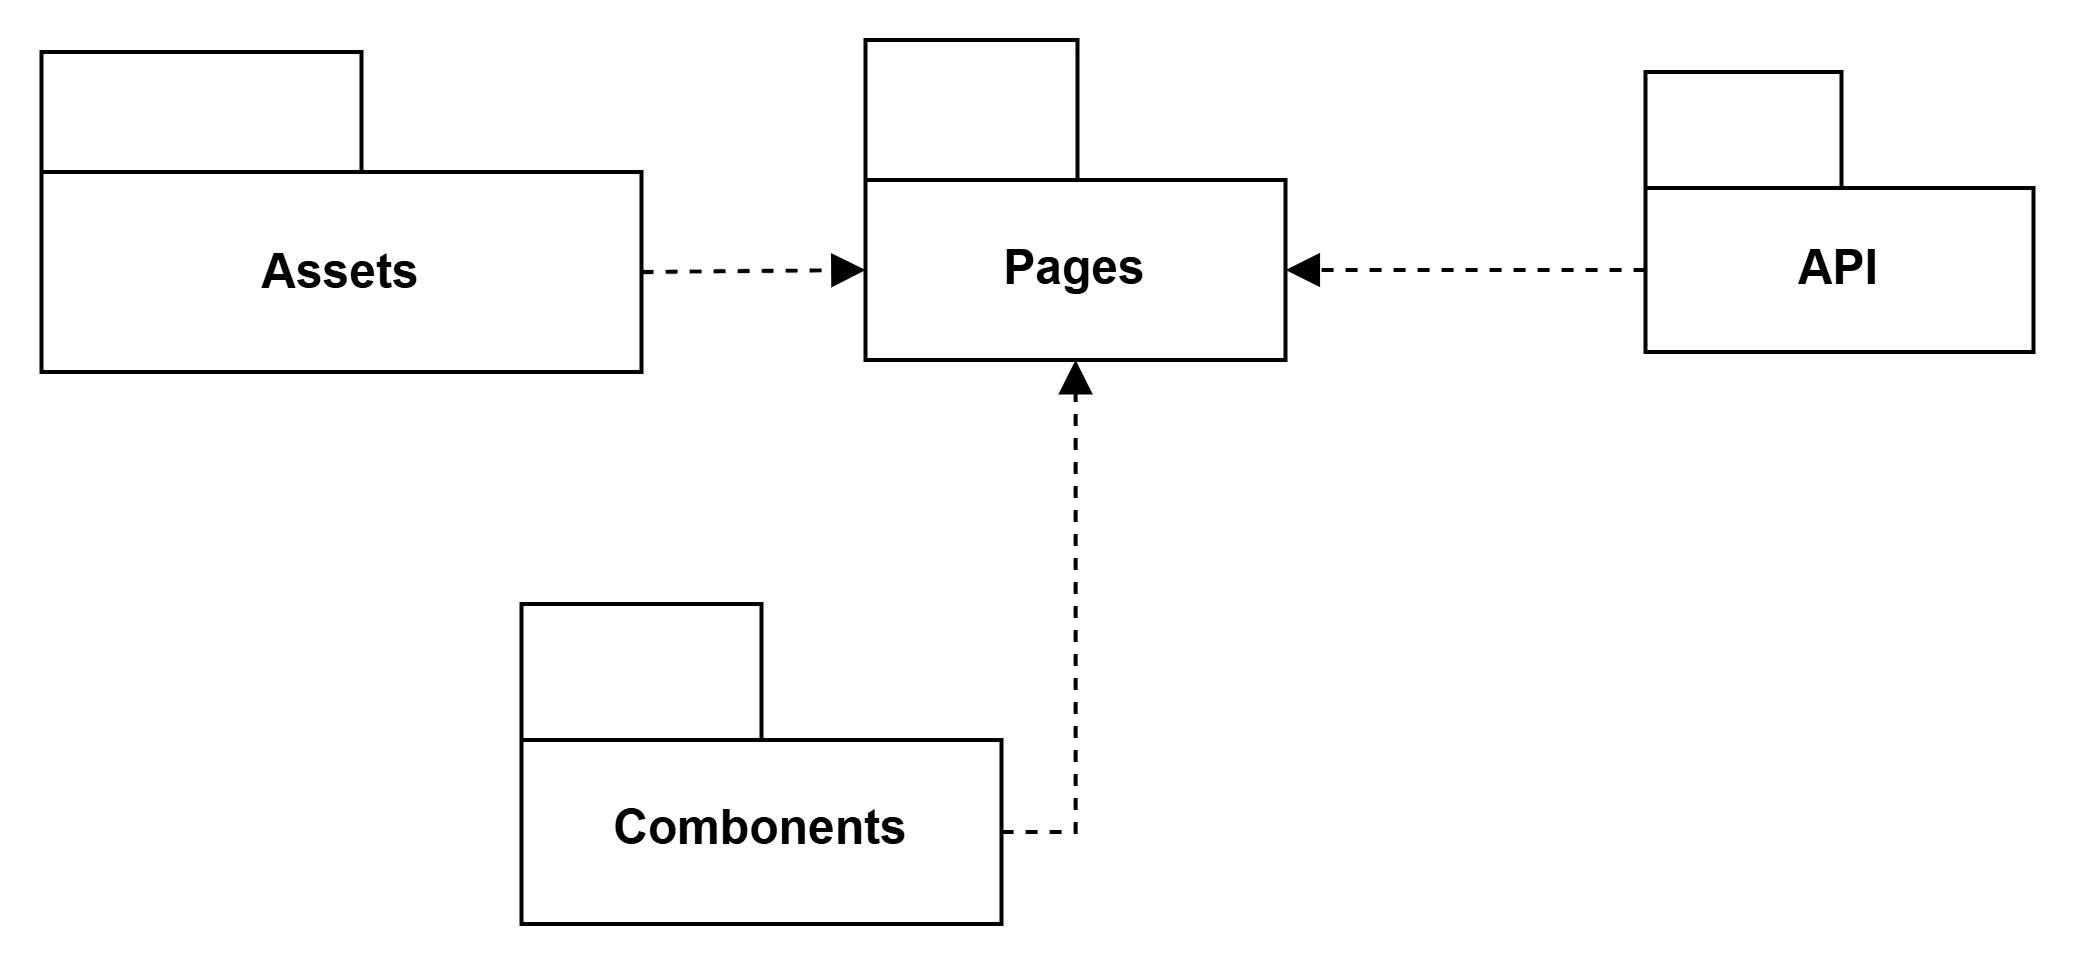
\includegraphics[width=\textwidth]{images/4.jpg}
	\caption{Package Diagram của Frontend}
	\label{fig:package-diagram-frontend}
\end{figure}

\begin{longtable}{
		|>{\raggedright\arraybackslash}p{0.8cm}|
		>{\raggedright\arraybackslash}p{4.0cm}|
		>{\raggedright\arraybackslash}p{8.0cm}|
	}
	\caption{Các package chính của Frontend}
	\label{tab:frontend-packages}\\
	\hline
	\textbf{No} & \textbf{Package} & \textbf{Description} \\ \hline
	\endfirsthead
	
	\hline
	\textbf{No} & \textbf{Package} & \textbf{Description} \\ \hline
	\endhead
	
	1 & frontend &
	Thư mục gốc chứa mã nguồn Frontend của ứng dụng Web. \\ \hline
	
	2 & authentication &
	Chứa các trang đăng nhập, đăng ký, xác thực OTP,
	quên mật khẩu và đặt lại mật khẩu. \\ \hline
	
	3 & photographer &
	Chứa các trang dành cho Photographer như trang chủ,
	tìm kiếm, hồ sơ, Booking, thanh toán, lịch sử,
	Workshop và thông báo. \\ \hline
	
	4 & provider &
	Chứa các trang dành cho Service Provider như Dashboard,
	hồ sơ, Creative Space, Equipment, Service Package,
	Booking và Workshop. \\ \hline
	
	5 & admin &
	Chứa các trang quản trị như Dashboard, quản lý người dùng,
	Provider, phê duyệt Provider và giao dịch. \\ \hline
	
	6 & components &
	Chứa các thành phần giao diện dùng chung như Navbar và Footer. \\ \hline
	
	7 & api &
	Chứa các module JavaScript hỗ trợ giao tiếp với REST API. \\ \hline
	
	8 & assets &
	Chứa các tài nguyên giao diện như CSS và hình ảnh. \\ \hline
	
\end{longtable}


\subsubsection{Backend}

\begin{figure}[H]
	\centering
	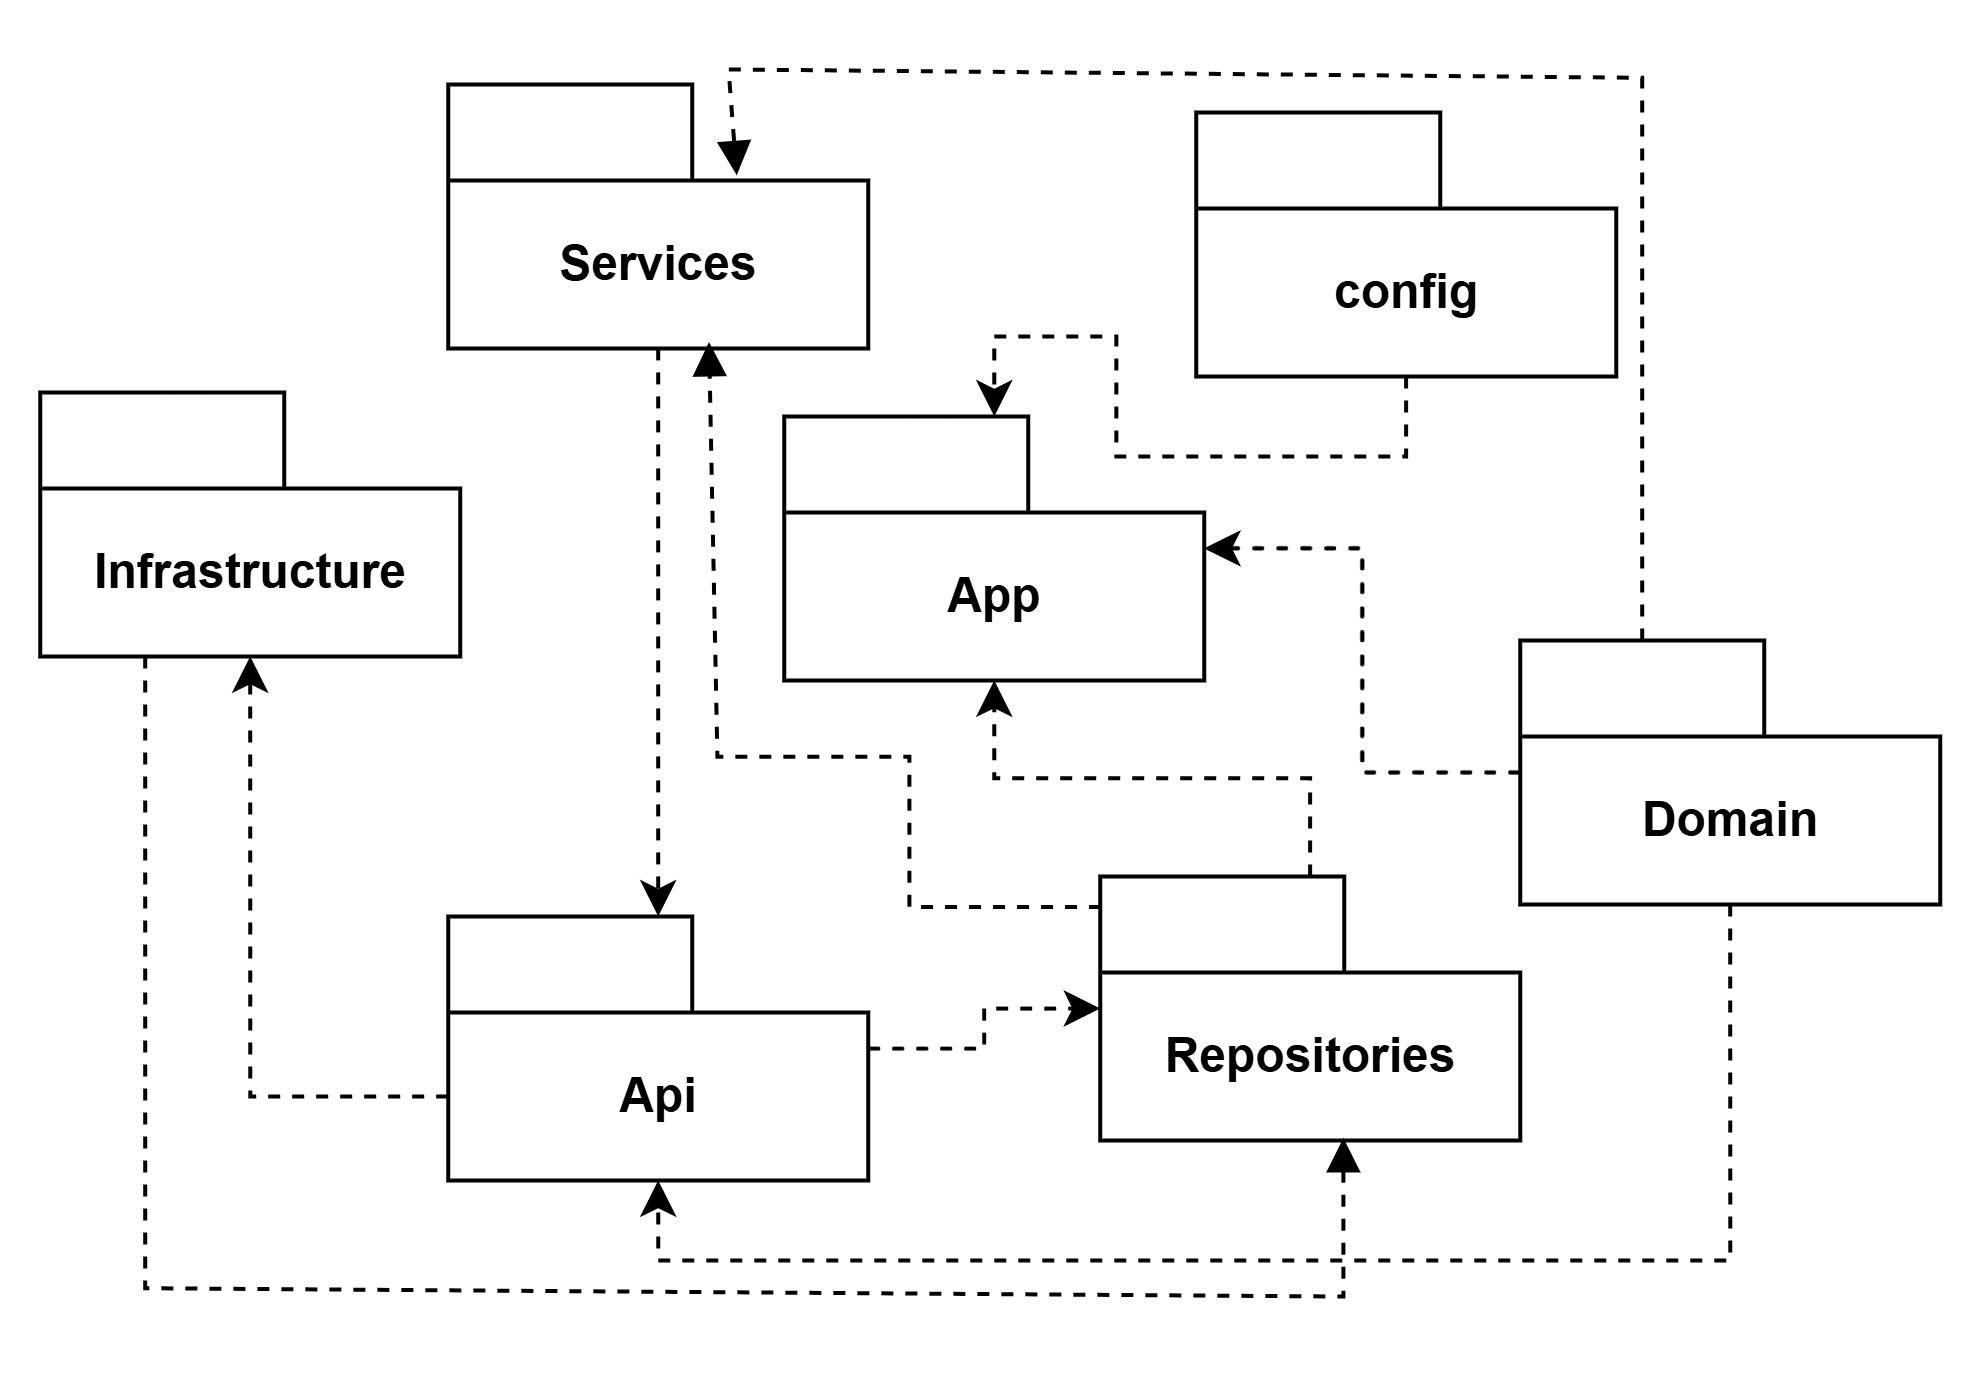
\includegraphics[width=\textwidth]{images/3.jpg}
	\caption{Package Diagram của Backend}
	\label{fig:package-diagram-backend}
\end{figure}

\begin{longtable}{
		|>{\raggedright\arraybackslash}p{0.8cm}|
		>{\raggedright\arraybackslash}p{4.0cm}|
		>{\raggedright\arraybackslash}p{8.0cm}|
	}
	\caption{Các package chính của Backend}
	\label{tab:backend-packages}\\
	\hline
	\textbf{No} & \textbf{Package} & \textbf{Description} \\ \hline
	\endfirsthead
	
	\hline
	\textbf{No} & \textbf{Package} & \textbf{Description} \\ \hline
	\endhead
	
	1 & src &
	Thư mục gốc chứa mã nguồn Backend của hệ thống. \\ \hline
	
	2 & src/api &
	Chứa Controllers, Schemas và các REST API endpoints. \\ \hline
	
	3 & src/services &
	Chứa xử lý nghiệp vụ cho Authentication, User, Creative Space,
	Equipment, Service Package, Booking, Workshop, Invoice,
	Payment, Notification và Provider. \\ \hline
	
	4 & src/domain &
	Chứa Domain Models, Repository Interfaces
	và các quy tắc nghiệp vụ cốt lõi. \\ \hline
	
	5 & src/infrastructure &
	Chứa các thành phần triển khai kỹ thuật
	và truy cập dữ liệu. \\ \hline
	
	6 & infrastructure /repositories &
	Chứa các Repository thực hiện truy xuất và thao tác dữ liệu. \\ \hline
	
	7 & infrastructure/models &
	Chứa các SQLAlchemy ORM Models và ánh xạ cơ sở dữ liệu. \\ \hline
	
	8 & infrastructure/databases &
	Chứa các thành phần quản lý kết nối và Database Session. \\ \hline
	
	9 & src/config.py &
	Chứa cấu hình ứng dụng và các thiết lập môi trường. \\ \hline
	
	10 & src/email\_service.py &
	Cung cấp dịch vụ Email cho OTP và khôi phục mật khẩu. \\ \hline
	
\end{longtable}

\section{Database Design}

Cơ sở dữ liệu của hệ thống được thiết kế theo mô hình quan hệ nhằm
đảm bảo tính nhất quán giữa tài khoản người dùng, Service Provider,
Creative Space, Equipment, Booking, Workshop, Invoice, Payment và
Notification. Các thực thể chính và mối quan hệ giữa chúng được thể hiện
trong sơ đồ Entity Relationship Diagram dưới đây.

\begin{figure}[H]
	\centering
	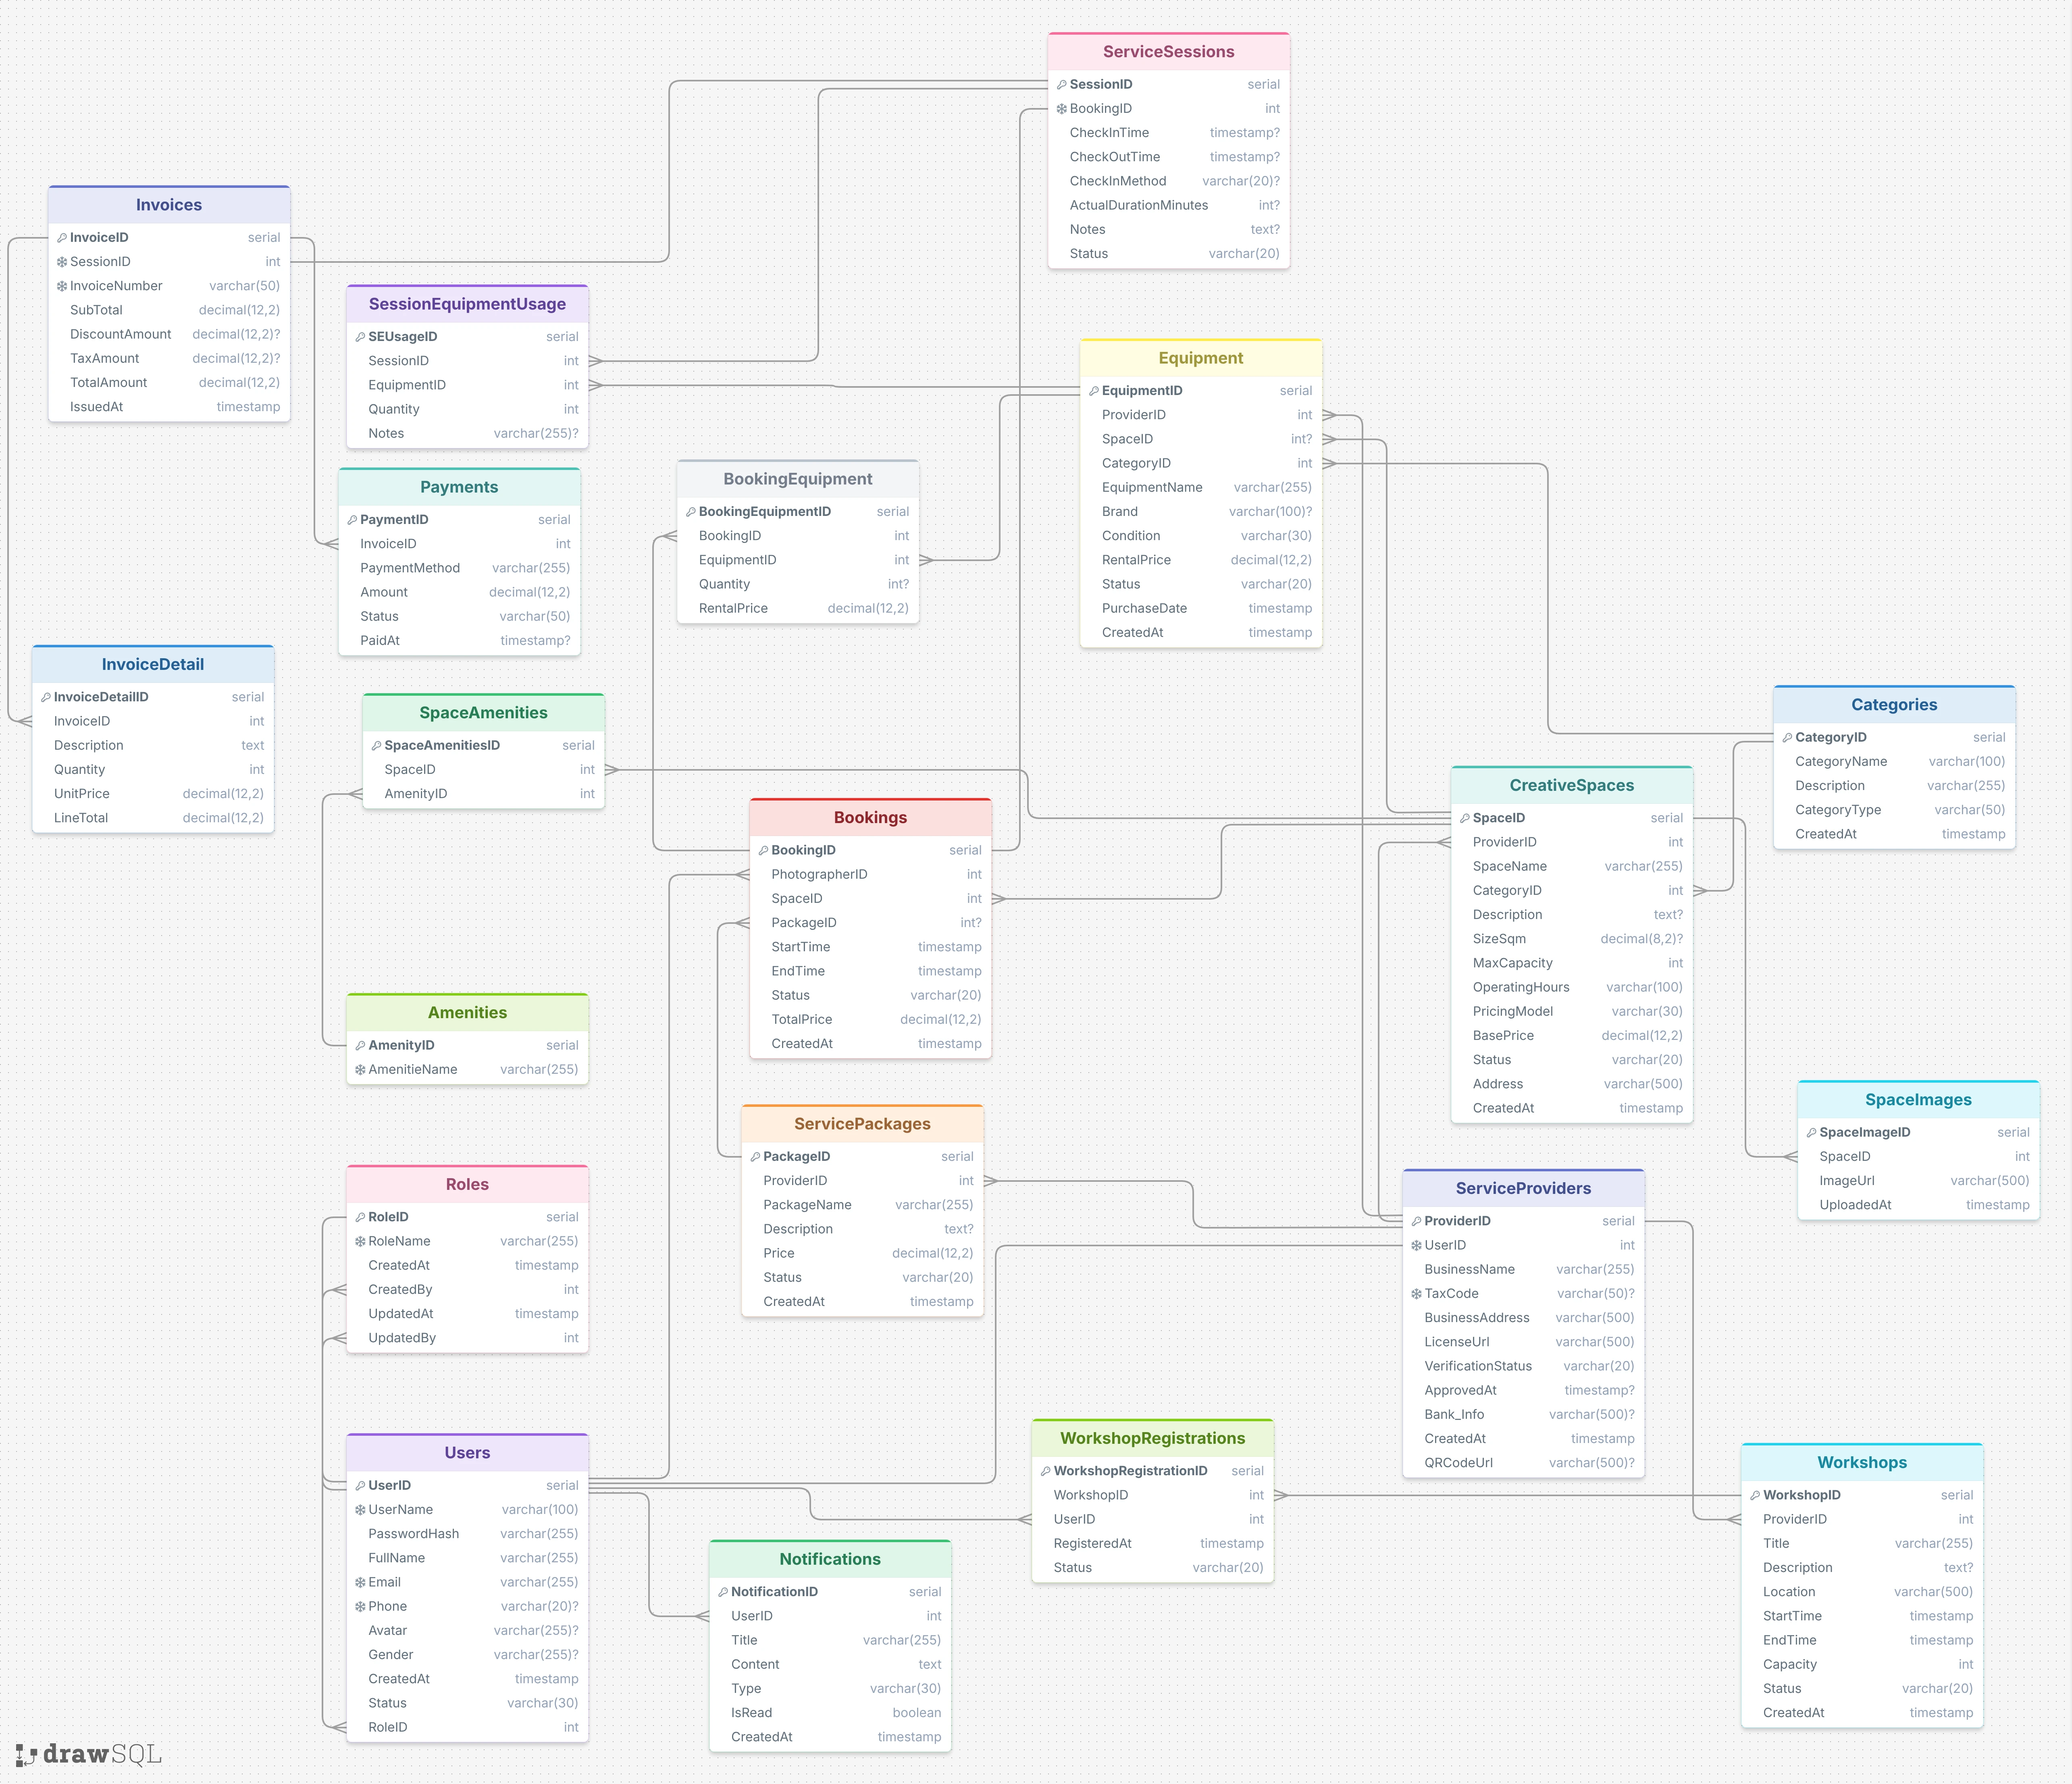
\includegraphics[width=\textwidth]{images/7.png}
	\caption{Entity Relationship Diagram}
	\label{fig:entity-relationship-diagram}
\end{figure}


\subsection{Database Tables Overview}

Cơ sở dữ liệu của hệ thống gồm 20 bảng chính. Các bảng hỗ trợ quản lý
tài khoản và phân quyền, Service Provider, Creative Space, Equipment,
Booking, Service Package, Service Session, Workshop, Invoice, Payment
và Notification.

\subsection{Users Table}

\begin{longtable}{
		|>{\raggedright\arraybackslash}p{3.2cm}|
		>{\raggedright\arraybackslash}p{4.2cm}|
		>{\raggedright\arraybackslash}p{5.0cm}|
	}
	\caption{Users Table Description}
	\label{tab:users}\\
	\hline
	\textbf{Field} & \textbf{Type} & \textbf{Description} \\ \hline
	\endfirsthead
	\hline
	\textbf{Field} & \textbf{Type} & \textbf{Description} \\ \hline
	\endhead
	
	UserID & INT, PK, IDENTITY &
	Unique identifier of the user account. \\ \hline
	
	UserName & VARCHAR(100), UNIQUE, NOT NULL &
	Username used to identify the account. \\ \hline
	
	PasswordHash & VARCHAR(255), NOT NULL &
	Hashed password of the user. \\ \hline
	
	FullName & VARCHAR(255), NOT NULL &
	Full name of the user. \\ \hline
	
	Email & VARCHAR(255), UNIQUE, NOT NULL &
	Email address of the user. \\ \hline
	
	Phone & VARCHAR(20), UNIQUE, NULL &
	Phone number of the user. \\ \hline
	
	Avatar & VARCHAR(255), NULL &
	Path or URL of the user's avatar. \\ \hline
	
	Gender & VARCHAR(255), NULL &
	Gender information of the user. \\ \hline
	
	CreatedAt & DATETIME, NOT NULL &
	Account creation time. \\ \hline
	
	Status & VARCHAR(30), NOT NULL &
	Current status of the user account. \\ \hline
	
	RoleID & INT, FK, NOT NULL &
	Reference to the user's role. \\ \hline
	
\end{longtable}


\subsection{Roles Table}

\begin{longtable}{
		|>{\raggedright\arraybackslash}p{3.2cm}|
		>{\raggedright\arraybackslash}p{4.2cm}|
		>{\raggedright\arraybackslash}p{5.0cm}|
	}
	\caption{Roles Table Description}
	\label{tab:roles}\\
	\hline
	\textbf{Field} & \textbf{Type} & \textbf{Description} \\ \hline
	\endfirsthead
	\hline
	\textbf{Field} & \textbf{Type} & \textbf{Description} \\ \hline
	\endhead
	
	RoleID & INT, PK, IDENTITY &
	Unique identifier of the role. \\ \hline
	
	RoleName & VARCHAR(255), UNIQUE, NOT NULL &
	Name of the user role. \\ \hline
	
	CreatedAt & DATETIME, NOT NULL &
	Role creation time. \\ \hline
	
	CreatedBy & INT, FK, NOT NULL &
	User who created the role. \\ \hline
	
	UpdatedAt & DATETIME, NOT NULL &
	Time when the role was last updated. \\ \hline
	
	UpdatedBy & INT, FK, NOT NULL &
	User who last updated the role. \\ \hline
	
\end{longtable}


\subsection{ServiceProviders Table}

\begin{longtable}{
		|>{\raggedright\arraybackslash}p{3.2cm}|
		>{\raggedright\arraybackslash}p{4.2cm}|
		>{\raggedright\arraybackslash}p{5.0cm}|
	}
	\caption{ServiceProviders Table Description}
	\label{tab:service-providers}\\
	\hline
	\textbf{Field} & \textbf{Type} & \textbf{Description} \\ \hline
	\endfirsthead
	\hline
	\textbf{Field} & \textbf{Type} & \textbf{Description} \\ \hline
	\endhead
	
	ProviderID & INT, PK, IDENTITY &
	Unique identifier of the Service Provider. \\ \hline
	
	UserID & INT, FK, UNIQUE, NOT NULL &
	Reference to the corresponding user account. \\ \hline
	
	BusinessName & VARCHAR(255), NOT NULL &
	Business name of the Service Provider. \\ \hline
	
	TaxCode & VARCHAR(50), UNIQUE, NULL &
	Tax identification code of the Service Provider. \\ \hline
	
	BusinessAddress & VARCHAR(500), NOT NULL &
	Business address of the Service Provider. \\ \hline
	
	LicenseUrl & VARCHAR(500), NOT NULL &
	URL of the business license document. \\ \hline
	
	VerificationStatus & VARCHAR(20), NOT NULL &
	Verification status of the Service Provider. \\ \hline
	
	ApprovedAt & DATETIME, NULL &
	Time when the Service Provider was approved. \\ \hline
	
	Bank\_Info & VARCHAR(500), NULL &
	Banking information of the Service Provider. \\ \hline
	
	CreatedAt & DATETIME, NOT NULL &
	Provider record creation time. \\ \hline
	
	QRCodeUrl & VARCHAR(500), NULL &
	URL of the payment QR code. \\ \hline
	
\end{longtable}


\subsection{Categories Table}

\begin{longtable}{
		|>{\raggedright\arraybackslash}p{3.2cm}|
		>{\raggedright\arraybackslash}p{4.2cm}|
		>{\raggedright\arraybackslash}p{5.0cm}|
	}
	\caption{Categories Table Description}
	\label{tab:categories}\\
	\hline
	\textbf{Field} & \textbf{Type} & \textbf{Description} \\ \hline
	\endfirsthead
	\hline
	\textbf{Field} & \textbf{Type} & \textbf{Description} \\ \hline
	\endhead
	
	CategoryID & INT, PK, IDENTITY &
	Unique identifier of the category. \\ \hline
	
	CategoryName & VARCHAR(100), NOT NULL &
	Name of the category. \\ \hline
	
	Description & VARCHAR(255), NOT NULL &
	Description of the category. \\ \hline
	
	CategoryType & VARCHAR(50), NOT NULL &
	Type of the category. \\ \hline
	
	CreatedAt & DATETIME, NOT NULL &
	Category creation time. \\ \hline
	
\end{longtable}


\subsection{CreativeSpaces Table}

\begin{longtable}{
		|>{\raggedright\arraybackslash}p{3.2cm}|
		>{\raggedright\arraybackslash}p{4.2cm}|
		>{\raggedright\arraybackslash}p{5.0cm}|
	}
	\caption{CreativeSpaces Table Description}
	\label{tab:creative-spaces}\\
	\hline
	\textbf{Field} & \textbf{Type} & \textbf{Description} \\ \hline
	\endfirsthead
	\hline
	\textbf{Field} & \textbf{Type} & \textbf{Description} \\ \hline
	\endhead
	
	SpaceID & INT, PK, IDENTITY &
	Unique identifier of the Creative Space. \\ \hline
	
	ProviderID & INT, FK, NOT NULL &
	Reference to the Service Provider. \\ \hline
	
	SpaceName & VARCHAR(255), NOT NULL &
	Name of the Creative Space. \\ \hline
	
	CategoryID & INT, FK, NOT NULL &
	Reference to the space category. \\ \hline
	
	Description & TEXT, NULL &
	Detailed description of the Creative Space. \\ \hline
	
	SizeSqm & NUMERIC(8,2), NULL &
	Area of the Creative Space in square meters. \\ \hline
	
	MaxCapacity & INT, NOT NULL &
	Maximum capacity of the Creative Space. \\ \hline
	
	OperatingHours & VARCHAR(100), NOT NULL &
	Operating hours of the Creative Space. \\ \hline
	
	PricingModel & VARCHAR(30), NOT NULL &
	Pricing model of the Creative Space. \\ \hline
	
	BasePrice & NUMERIC(12,2), NOT NULL &
	Base price of the Creative Space. \\ \hline
	
	Status & VARCHAR(20), NOT NULL &
	Current status of the Creative Space. \\ \hline
	
	Address & VARCHAR(500), NOT NULL &
	Address of the Creative Space. \\ \hline
	
	CreatedAt & DATETIME, NOT NULL &
	Space creation time. \\ \hline
	
\end{longtable}


\subsection{SpaceImages Table}

\begin{longtable}{
		|>{\raggedright\arraybackslash}p{3.2cm}|
		>{\raggedright\arraybackslash}p{4.2cm}|
		>{\raggedright\arraybackslash}p{5.0cm}|
	}
	\caption{SpaceImages Table Description}
	\label{tab:space-images}\\
	\hline
	\textbf{Field} & \textbf{Type} & \textbf{Description} \\ \hline
	\endfirsthead
	\hline
	\textbf{Field} & \textbf{Type} & \textbf{Description} \\ \hline
	\endhead
	
	SpaceImageID & INT, PK, IDENTITY &
	Unique identifier of the space image. \\ \hline
	
	SpaceID & INT, FK, NOT NULL &
	Reference to the Creative Space. \\ \hline
	
	ImageUrl & VARCHAR(500), NOT NULL &
	URL of the Creative Space image. \\ \hline
	
	UploadedAt & DATETIME, NOT NULL &
	Image upload time. \\ \hline
	
\end{longtable}


\subsection{Amenities Table}

\begin{longtable}{
		|>{\raggedright\arraybackslash}p{3.2cm}|
		>{\raggedright\arraybackslash}p{4.2cm}|
		>{\raggedright\arraybackslash}p{5.0cm}|
	}
	\caption{Amenities Table Description}
	\label{tab:amenities}\\
	\hline
	\textbf{Field} & \textbf{Type} & \textbf{Description} \\ \hline
	\endfirsthead
	\hline
	\textbf{Field} & \textbf{Type} & \textbf{Description} \\ \hline
	\endhead
	
	AmenityID & INT, PK, IDENTITY &
	Unique identifier of the amenity. \\ \hline
	
	AmenitieName & VARCHAR(255), UNIQUE, NOT NULL &
	Name of the amenity. \\ \hline
	
\end{longtable}


\subsection{SpaceAmenities Table}

\begin{longtable}{
		|>{\raggedright\arraybackslash}p{3.2cm}|
		>{\raggedright\arraybackslash}p{4.2cm}|
		>{\raggedright\arraybackslash}p{5.0cm}|
	}
	\caption{SpaceAmenities Table Description}
	\label{tab:space-amenities}\\
	\hline
	\textbf{Field} & \textbf{Type} & \textbf{Description} \\ \hline
	\endfirsthead
	\hline
	\textbf{Field} & \textbf{Type} & \textbf{Description} \\ \hline
	\endhead
	
	SpaceAmenitiesID & INT, PK, IDENTITY &
	Unique identifier of the space-amenity record. \\ \hline
	
	SpaceID & INT, FK, NOT NULL &
	Reference to the Creative Space. \\ \hline
	
	AmenityID & INT, FK, NOT NULL &
	Reference to the amenity. \\ \hline
	
\end{longtable}


\subsection{Equipment Table}

\begin{longtable}{
		|>{\raggedright\arraybackslash}p{3.2cm}|
		>{\raggedright\arraybackslash}p{4.2cm}|
		>{\raggedright\arraybackslash}p{5.0cm}|
	}
	\caption{Equipment Table Description}
	\label{tab:equipment}\\
	\hline
	\textbf{Field} & \textbf{Type} & \textbf{Description} \\ \hline
	\endfirsthead
	\hline
	\textbf{Field} & \textbf{Type} & \textbf{Description} \\ \hline
	\endhead
	
	EquipmentID & INT, PK, IDENTITY &
	Unique identifier of the equipment. \\ \hline
	
	ProviderID & INT, FK, NOT NULL &
	Reference to the Service Provider. \\ \hline
	
	SpaceID & INT, FK, NULL &
	Reference to the Creative Space associated with the equipment. \\ \hline
	
	CategoryID & INT, FK, NOT NULL &
	Reference to the equipment category. \\ \hline
	
	EquipmentName & VARCHAR(255), NOT NULL &
	Name of the equipment. \\ \hline
	
	Brand & VARCHAR(100), NULL &
	Brand of the equipment. \\ \hline
	
	Condition & VARCHAR(30), NOT NULL &
	Current physical condition of the equipment. \\ \hline
	
	RentalPrice & NUMERIC(12,2), NOT NULL &
	Rental price of the equipment. \\ \hline
	
	Status & VARCHAR(20), NOT NULL &
	Current status of the equipment. \\ \hline
	
	PurchaseDate & DATETIME, NOT NULL &
	Purchase date of the equipment. \\ \hline
	
	CreatedAt & DATETIME, NOT NULL &
	Equipment creation time. \\ \hline
	
\end{longtable}


\subsection{Bookings Table}

\begin{longtable}{
		|>{\raggedright\arraybackslash}p{3.2cm}|
		>{\raggedright\arraybackslash}p{4.2cm}|
		>{\raggedright\arraybackslash}p{5.0cm}|
	}
	\caption{Bookings Table Description}
	\label{tab:bookings}\\
	\hline
	\textbf{Field} & \textbf{Type} & \textbf{Description} \\ \hline
	\endfirsthead
	\hline
	\textbf{Field} & \textbf{Type} & \textbf{Description} \\ \hline
	\endhead
	
	BookingID & INT, PK, IDENTITY &
	Unique identifier of the Booking. \\ \hline
	
	PhotographerID & INT, FK, NOT NULL &
	Reference to the Photographer user. \\ \hline
	
	SpaceID & INT, FK, NOT NULL &
	Reference to the booked Creative Space. \\ \hline
	
	PackageID & INT, FK, NULL &
	Reference to the selected Service Package. \\ \hline
	
	StartTime & DATETIME, NOT NULL &
	Booking start time. \\ \hline
	
	EndTime & DATETIME, NOT NULL &
	Booking end time. \\ \hline
	
	Status & VARCHAR(20), NOT NULL &
	Current status of the Booking. \\ \hline
	
	TotalPrice & NUMERIC(12,2), NOT NULL &
	Total price of the Booking. \\ \hline
	
	CreatedAt & DATETIME, NOT NULL &
	Booking creation time. \\ \hline
	
\end{longtable}


\subsection{BookingEquipment Table}

\begin{longtable}{
		|>{\raggedright\arraybackslash}p{3.2cm}|
		>{\raggedright\arraybackslash}p{4.2cm}|
		>{\raggedright\arraybackslash}p{5.0cm}|
	}
	\caption{BookingEquipment Table Description}
	\label{tab:booking-equipment}\\
	\hline
	\textbf{Field} & \textbf{Type} & \textbf{Description} \\ \hline
	\endfirsthead
	\hline
	\textbf{Field} & \textbf{Type} & \textbf{Description} \\ \hline
	\endhead
	
	BookingEquipmentID & INT, PK, IDENTITY &
	Unique identifier of the Booking equipment record. \\ \hline
	
	BookingID & INT, FK, NOT NULL &
	Reference to the Booking. \\ \hline
	
	EquipmentID & INT, FK, NOT NULL &
	Reference to the selected equipment. \\ \hline
	
	Quantity & INT, NULL &
	Quantity of the selected equipment. \\ \hline
	
	RentalPrice & NUMERIC(12,2), NOT NULL &
	Rental price of the equipment. \\ \hline
	
\end{longtable}


\subsection{ServiceSessions Table}

\begin{longtable}{
		|>{\raggedright\arraybackslash}p{3.2cm}|
		>{\raggedright\arraybackslash}p{4.2cm}|
		>{\raggedright\arraybackslash}p{5.0cm}|
	}
	\caption{ServiceSessions Table Description}
	\label{tab:service-sessions}\\
	\hline
	\textbf{Field} & \textbf{Type} & \textbf{Description} \\ \hline
	\endfirsthead
	\hline
	\textbf{Field} & \textbf{Type} & \textbf{Description} \\ \hline
	\endhead
	
	SessionID & INT, PK, IDENTITY &
	Unique identifier of the service session. \\ \hline
	
	BookingID & INT, FK, UNIQUE, NOT NULL &
	Reference to the Booking. \\ \hline
	
	CheckInTime & DATETIME, NULL &
	Check-in time of the Photographer. \\ \hline
	
	CheckOutTime & DATETIME, NULL &
	Check-out time of the Photographer. \\ \hline
	
	CheckInMethod & VARCHAR(20), NULL &
	Method used for check-in. \\ \hline
	
	ActualDurationMinutes & INT, NULL &
	Actual service duration in minutes. \\ \hline
	
	Notes & TEXT, NULL &
	Additional notes about the service session. \\ \hline
	
	Status & VARCHAR(20), NOT NULL &
	Current status of the service session. \\ \hline
	
\end{longtable}


\subsection{SessionEquipmentUsage Table}

\begin{longtable}{
		|>{\raggedright\arraybackslash}p{3.2cm}|
		>{\raggedright\arraybackslash}p{4.2cm}|
		>{\raggedright\arraybackslash}p{5.0cm}|
	}
	\caption{SessionEquipmentUsage Table Description}
	\label{tab:session-equipment-usage}\\
	\hline
	\textbf{Field} & \textbf{Type} & \textbf{Description} \\ \hline
	\endfirsthead
	\hline
	\textbf{Field} & \textbf{Type} & \textbf{Description} \\ \hline
	\endhead
	
	SEUsageID & INT, PK, IDENTITY &
	Unique identifier of the equipment usage record. \\ \hline
	
	SessionID & INT, FK, NOT NULL &
	Reference to the service session. \\ \hline
	
	EquipmentID & INT, FK, NOT NULL &
	Reference to the used equipment. \\ \hline
	
	Quantity & INT, NOT NULL &
	Quantity of equipment used. \\ \hline
	
	Notes & VARCHAR(255), NULL &
	Additional notes about equipment usage. \\ \hline
	
\end{longtable}


\subsection{ServicePackages Table}

\begin{longtable}{
		|>{\raggedright\arraybackslash}p{3.2cm}|
		>{\raggedright\arraybackslash}p{4.2cm}|
		>{\raggedright\arraybackslash}p{5.0cm}|
	}
	\caption{ServicePackages Table Description}
	\label{tab:service-packages}\\
	\hline
	\textbf{Field} & \textbf{Type} & \textbf{Description} \\ \hline
	\endfirsthead
	\hline
	\textbf{Field} & \textbf{Type} & \textbf{Description} \\ \hline
	\endhead
	
	PackageID & INT, PK, IDENTITY &
	Unique identifier of the Service Package. \\ \hline
	
	ProviderID & INT, FK, NOT NULL &
	Reference to the Service Provider. \\ \hline
	
	PackageName & VARCHAR(255), NOT NULL &
	Name of the Service Package. \\ \hline
	
	Description & TEXT, NULL &
	Description of the Service Package. \\ \hline
	
	Price & NUMERIC(12,2), NOT NULL &
	Price of the Service Package. \\ \hline
	
	Status & VARCHAR(20), NOT NULL &
	Current status of the Service Package. \\ \hline
	
	CreatedAt & DATETIME, NOT NULL &
	Package creation time. \\ \hline
	
\end{longtable}


\subsection{Invoices Table}

\begin{longtable}{
		|>{\raggedright\arraybackslash}p{3.2cm}|
		>{\raggedright\arraybackslash}p{4.2cm}|
		>{\raggedright\arraybackslash}p{5.0cm}|
	}
	\caption{Invoices Table Description}
	\label{tab:invoices}\\
	\hline
	\textbf{Field} & \textbf{Type} & \textbf{Description} \\ \hline
	\endfirsthead
	\hline
	\textbf{Field} & \textbf{Type} & \textbf{Description} \\ \hline
	\endhead
	
	InvoiceID & INT, PK, IDENTITY &
	Unique identifier of the invoice. \\ \hline
	
	SessionID & INT, FK, UNIQUE, NOT NULL &
	Reference to the service session. \\ \hline
	
	InvoiceNumber & VARCHAR(50), UNIQUE, NOT NULL &
	Unique invoice number. \\ \hline
	
	SubTotal & NUMERIC(12,2), NOT NULL &
	Subtotal amount before discount and tax. \\ \hline
	
	DiscountAmount & NUMERIC(12,2), NULL &
	Discount amount applied to the invoice. \\ \hline
	
	TaxAmount & NUMERIC(12,2), NULL &
	Tax amount applied to the invoice. \\ \hline
	
	TotalAmount & NUMERIC(12,2), NOT NULL &
	Final total amount of the invoice. \\ \hline
	
	IssuedAt & DATETIME, NOT NULL &
	Invoice issue time. \\ \hline
	
\end{longtable}


\subsection{InvoiceDetail Table}

\begin{longtable}{
		|>{\raggedright\arraybackslash}p{3.2cm}|
		>{\raggedright\arraybackslash}p{4.2cm}|
		>{\raggedright\arraybackslash}p{5.0cm}|
	}
	\caption{InvoiceDetail Table Description}
	\label{tab:invoice-detail}\\
	\hline
	\textbf{Field} & \textbf{Type} & \textbf{Description} \\ \hline
	\endfirsthead
	\hline
	\textbf{Field} & \textbf{Type} & \textbf{Description} \\ \hline
	\endhead
	
	InvoiceDetailID & INT, PK, IDENTITY &
	Unique identifier of the invoice detail. \\ \hline
	
	InvoiceID & INT, FK, NOT NULL &
	Reference to the invoice. \\ \hline
	
	Description & TEXT, NOT NULL &
	Description of the invoice item. \\ \hline
	
	Quantity & INT, NOT NULL &
	Quantity of the invoice item. \\ \hline
	
	UnitPrice & NUMERIC(12,2), NOT NULL &
	Unit price of the invoice item. \\ \hline
	
	LineTotal & NUMERIC(12,2), NOT NULL &
	Total amount of the invoice item. \\ \hline
	
\end{longtable}


\subsection{Payments Table}

\begin{longtable}{
		|>{\raggedright\arraybackslash}p{3.2cm}|
		>{\raggedright\arraybackslash}p{4.2cm}|
		>{\raggedright\arraybackslash}p{5.0cm}|
	}
	\caption{Payments Table Description}
	\label{tab:payments}\\
	\hline
	\textbf{Field} & \textbf{Type} & \textbf{Description} \\ \hline
	\endfirsthead
	\hline
	\textbf{Field} & \textbf{Type} & \textbf{Description} \\ \hline
	\endhead
	
	PaymentID & INT, PK, IDENTITY &
	Unique identifier of the payment. \\ \hline
	
	InvoiceID & INT, FK, NOT NULL &
	Reference to the invoice being paid. \\ \hline
	
	PaymentMethod & VARCHAR(255), NOT NULL &
	Payment method used by the Photographer. \\ \hline
	
	Amount & NUMERIC(12,2), NOT NULL &
	Payment amount. \\ \hline
	
	Status & VARCHAR(50), NOT NULL &
	Current status of the payment. \\ \hline
	
	PaidAt & DATETIME, NULL &
	Time when the payment was completed. \\ \hline
	
\end{longtable}


\subsection{Workshops Table}

\begin{longtable}{
		|>{\raggedright\arraybackslash}p{3.2cm}|
		>{\raggedright\arraybackslash}p{4.2cm}|
		>{\raggedright\arraybackslash}p{5.0cm}|
	}
	\caption{Workshops Table Description}
	\label{tab:workshops}\\
	\hline
	\textbf{Field} & \textbf{Type} & \textbf{Description} \\ \hline
	\endfirsthead
	\hline
	\textbf{Field} & \textbf{Type} & \textbf{Description} \\ \hline
	\endhead
	
	WorkshopID & INT, PK, IDENTITY &
	Unique identifier of the Workshop. \\ \hline
	
	ProviderID & INT, FK, NOT NULL &
	Reference to the Service Provider. \\ \hline
	
	Title & VARCHAR(255), NOT NULL &
	Workshop title. \\ \hline
	
	Description & TEXT, NULL &
	Detailed Workshop description. \\ \hline
	
	Location & VARCHAR(500), NOT NULL &
	Workshop location. \\ \hline
	
	StartTime & DATETIME, NOT NULL &
	Workshop start time. \\ \hline
	
	EndTime & DATETIME, NOT NULL &
	Workshop end time. \\ \hline
	
	Capacity & INT, NOT NULL &
	Maximum number of participants. \\ \hline
	
	Status & VARCHAR(20), NOT NULL &
	Current status of the Workshop. \\ \hline
	
	CreatedAt & DATETIME, NOT NULL &
	Workshop creation time. \\ \hline
	
\end{longtable}


\subsection{WorkshopRegistrations Table}

\begin{longtable}{
		|>{\raggedright\arraybackslash}p{3.2cm}|
		>{\raggedright\arraybackslash}p{4.2cm}|
		>{\raggedright\arraybackslash}p{5.0cm}|
	}
	\caption{WorkshopRegistrations Table Description}
	\label{tab:workshop-registrations}\\
	\hline
	\textbf{Field} & \textbf{Type} & \textbf{Description} \\ \hline
	\endfirsthead
	\hline
	\textbf{Field} & \textbf{Type} & \textbf{Description} \\ \hline
	\endhead
	
	WorkshopRegistrationID & INT, PK, IDENTITY &
	Unique identifier of the Workshop registration. \\ \hline
	
	WorkshopID & INT, FK, NOT NULL &
	Reference to the Workshop. \\ \hline
	
	UserID & INT, FK, NOT NULL &
	Reference to the registered Photographer. \\ \hline
	
	RegisteredAt & DATETIME, NOT NULL &
	Registration time. \\ \hline
	
	Status & VARCHAR(20), NOT NULL &
	Current status of the registration. \\ \hline
	
\end{longtable}


\subsection{Notifications Table}

\begin{longtable}{
		|>{\raggedright\arraybackslash}p{3.2cm}|
		>{\raggedright\arraybackslash}p{4.2cm}|
		>{\raggedright\arraybackslash}p{5.0cm}|
	}
	\caption{Notifications Table Description}
	\label{tab:notifications}\\
	\hline
	\textbf{Field} & \textbf{Type} & \textbf{Description} \\ \hline
	\endfirsthead
	\hline
	\textbf{Field} & \textbf{Type} & \textbf{Description} \\ \hline
	\endhead
	
	NotificationID & INT, PK, IDENTITY &
	Unique identifier of the notification. \\ \hline
	
	UserID & INT, FK, NOT NULL &
	Reference to the user receiving the notification. \\ \hline
	
	Title & VARCHAR(255), NOT NULL &
	Notification title. \\ \hline
	
	Content & TEXT, NOT NULL &
	Notification content. \\ \hline
	
	Type & VARCHAR(30), NOT NULL &
	Type of the notification. \\ \hline
	
	IsRead & BOOLEAN, NOT NULL &
	Indicates whether the notification has been read. \\ \hline
	
	CreatedAt & DATETIME, NOT NULL &
	Notification creation time. \\ \hline
	
\end{longtable}

\section{Chi tiết thiết kế}

Thiết kế chi tiết được xây dựng cho 34 Use Case được xác định trong
Chương III. Mỗi Use Case được phân tích dựa trên Actor, các thành phần
xử lý, cơ sở dữ liệu và luồng thực hiện tương ứng. Nội dung thiết kế
được tổ chức theo từng nhóm chức năng, bảo đảm sự thống nhất với kiến
trúc hệ thống, Package Design và Database Design được trình bày trong
các phần trước.

```latex
% =========================================================
% 3.1 Authentication Module
% =========================================================

\subsection{Authentication Module}

\subsubsection{Đăng ký Photographer}

\paragraph{Class Diagram}

\begin{figure}[H]
	\centering
	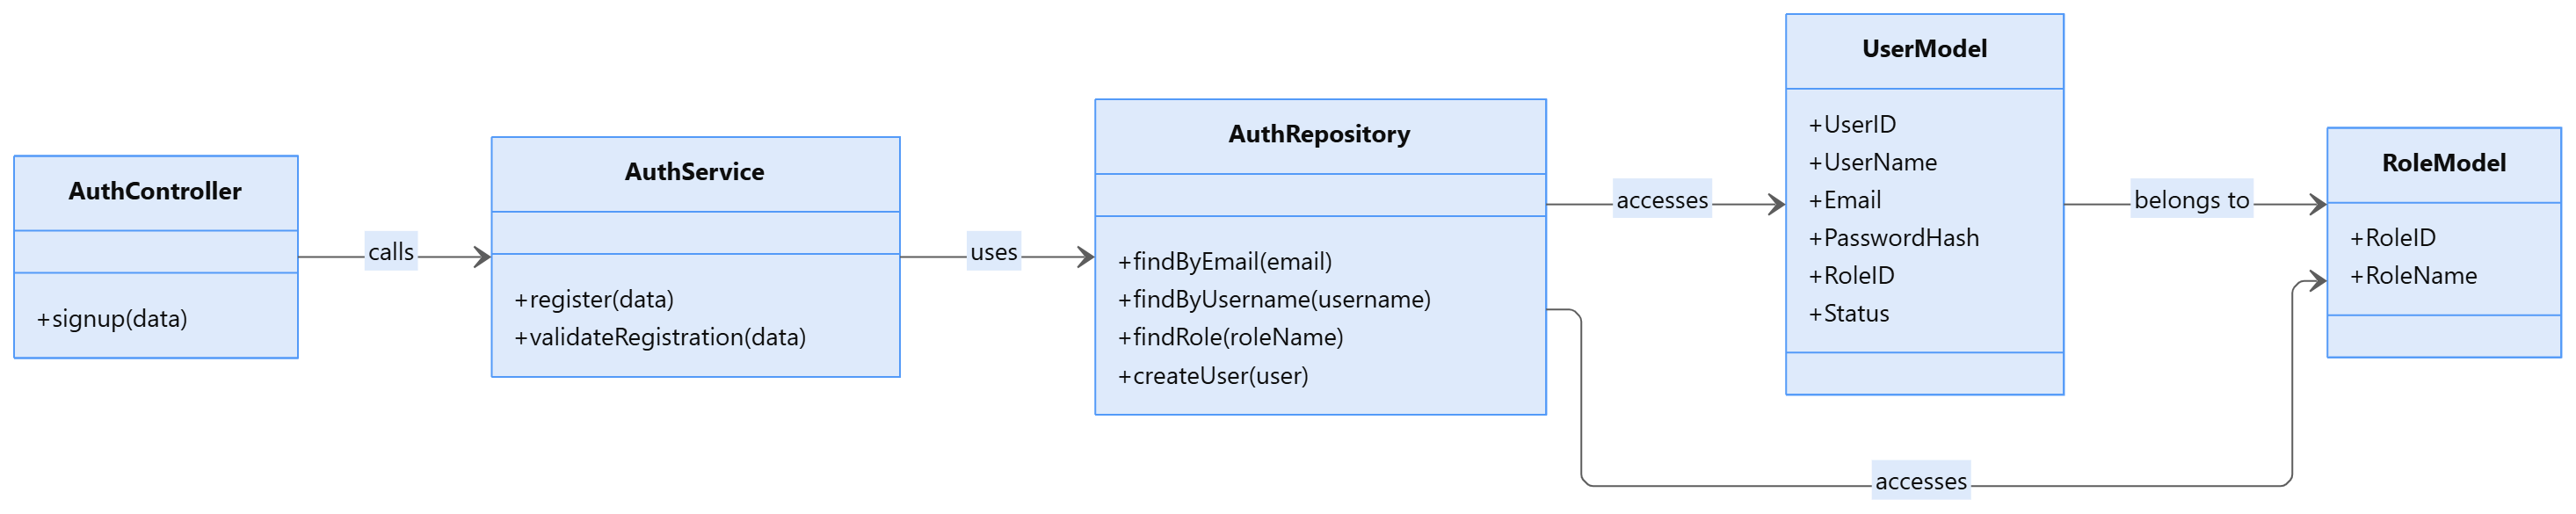
\includegraphics[width=1.1\textwidth]{images/12.png}
\end{figure}

\paragraph{Sequence Diagram}

\begin{figure}[H]
	\centering
	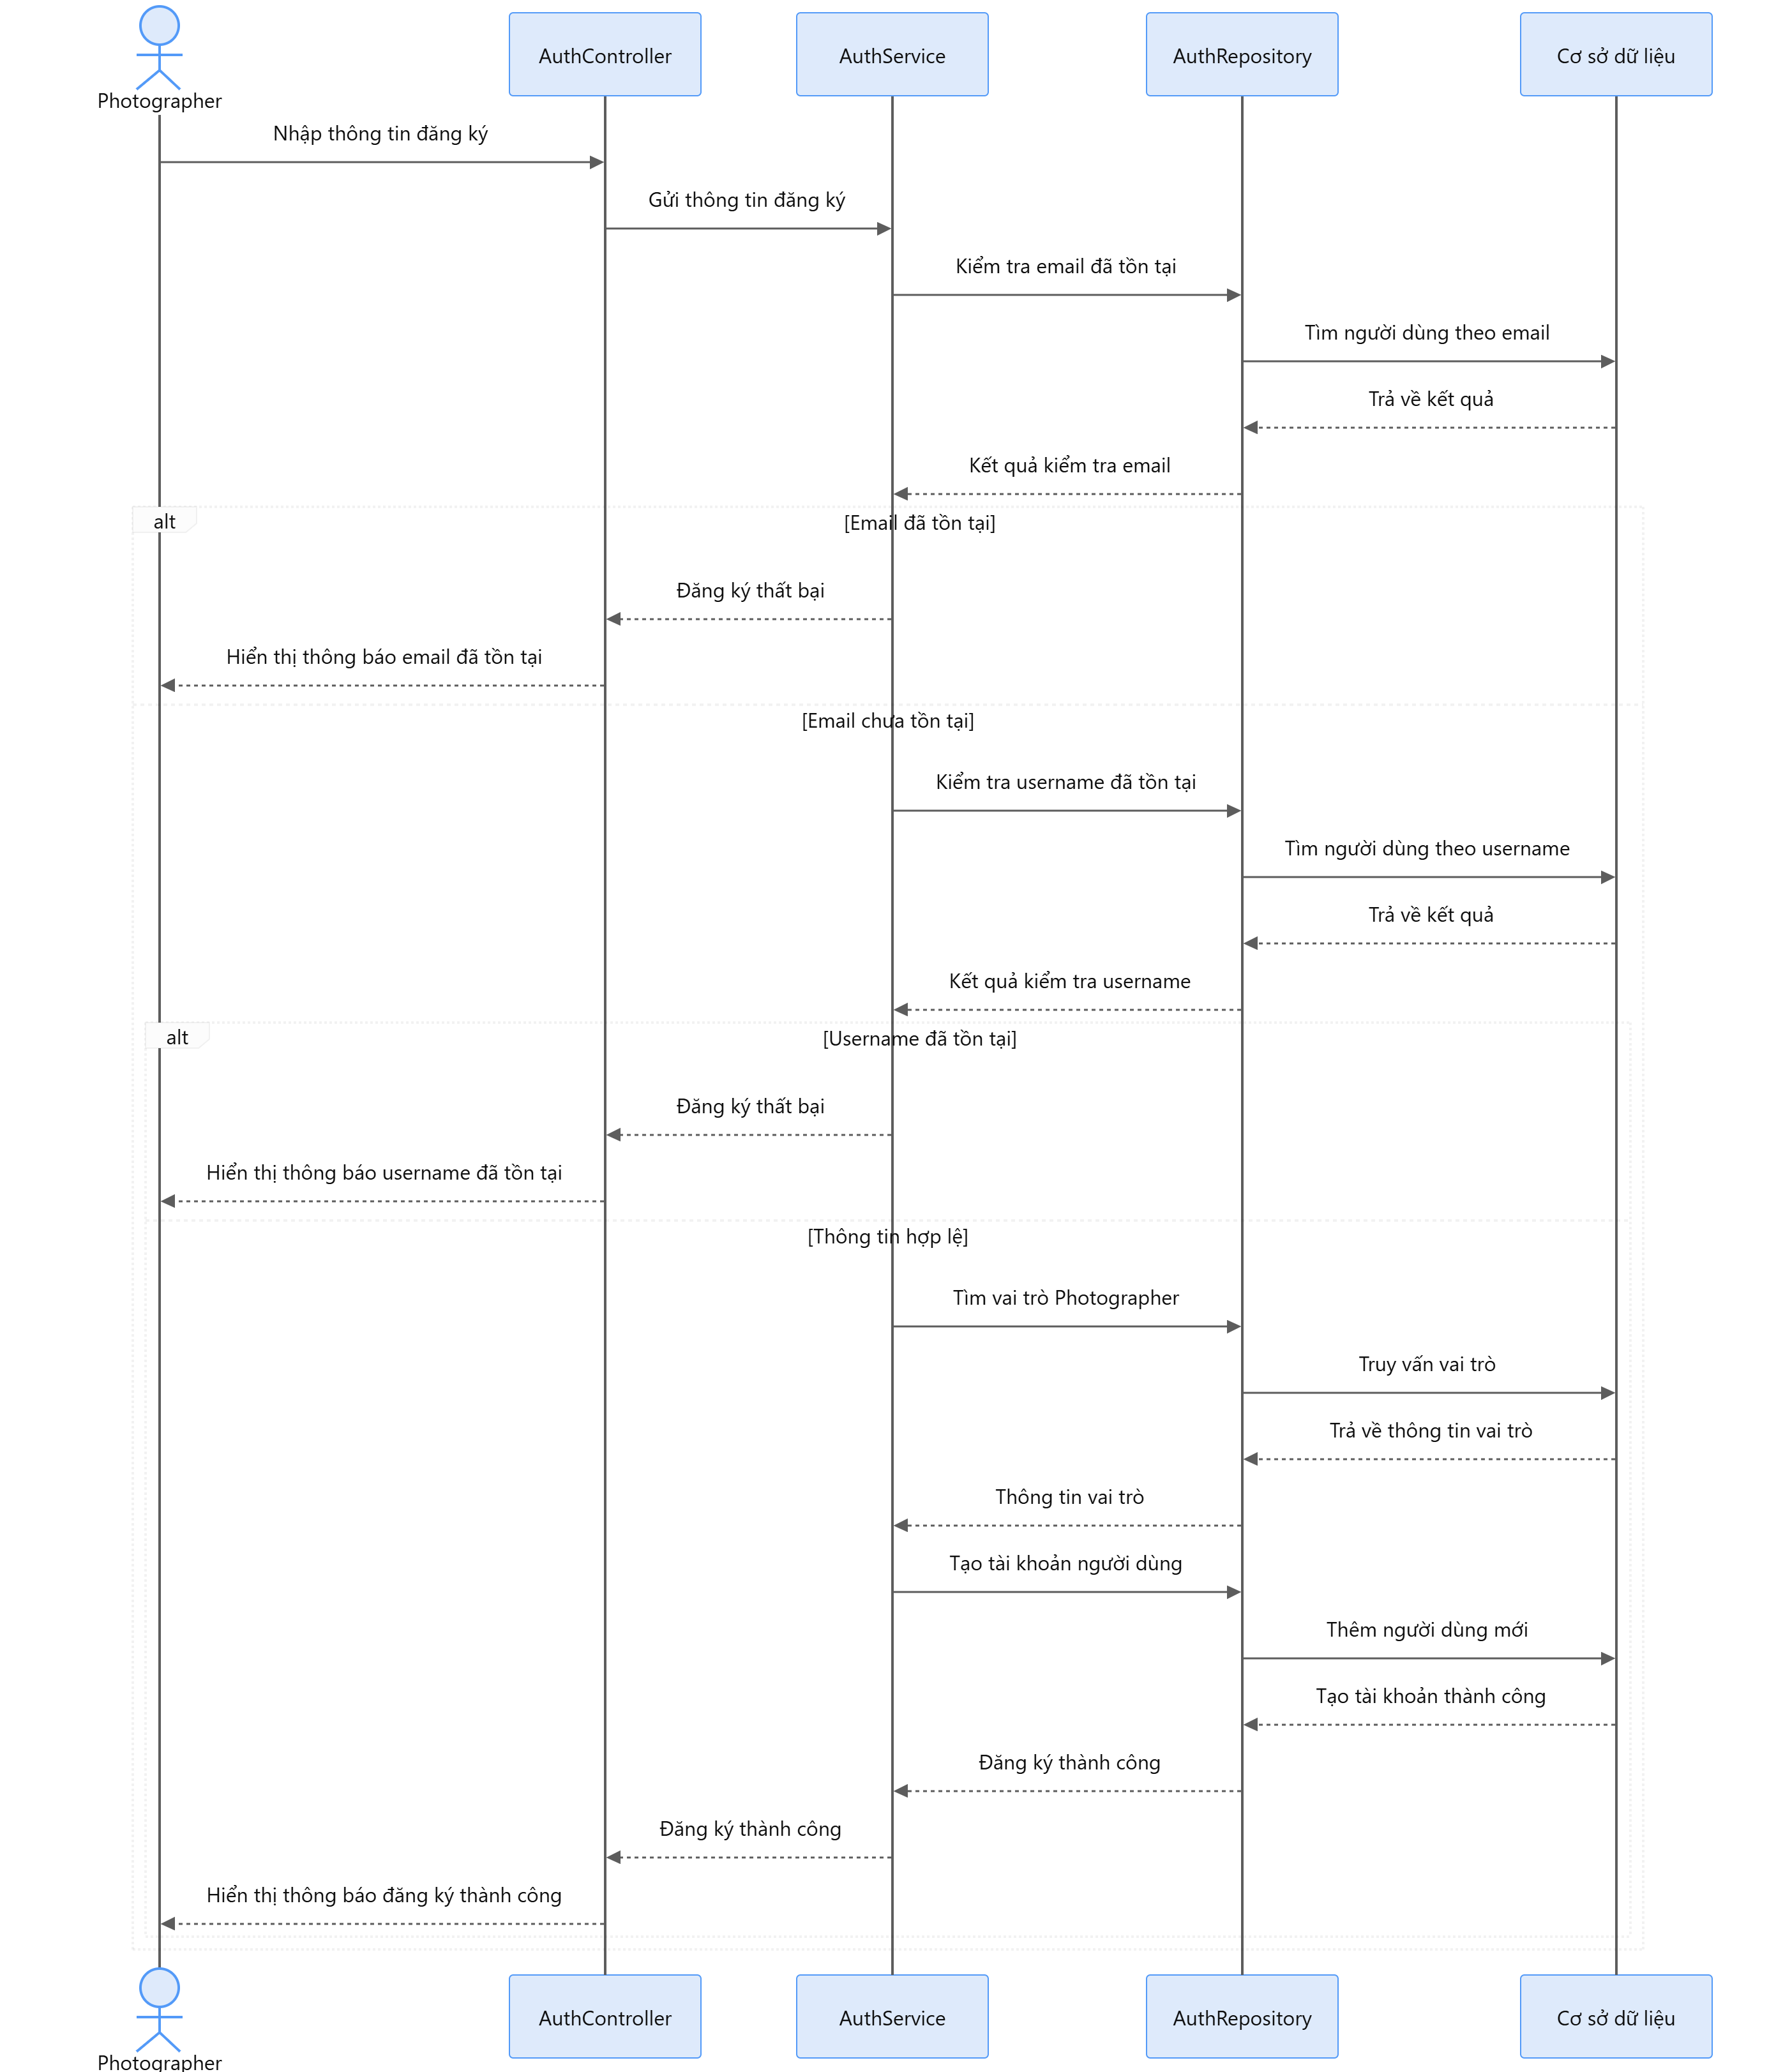
\includegraphics[width=1.1\textwidth]{images/13.png}
\end{figure}


\subsubsection{Đăng nhập}

\paragraph{Class Diagram}

\begin{figure}[H]
	\centering
	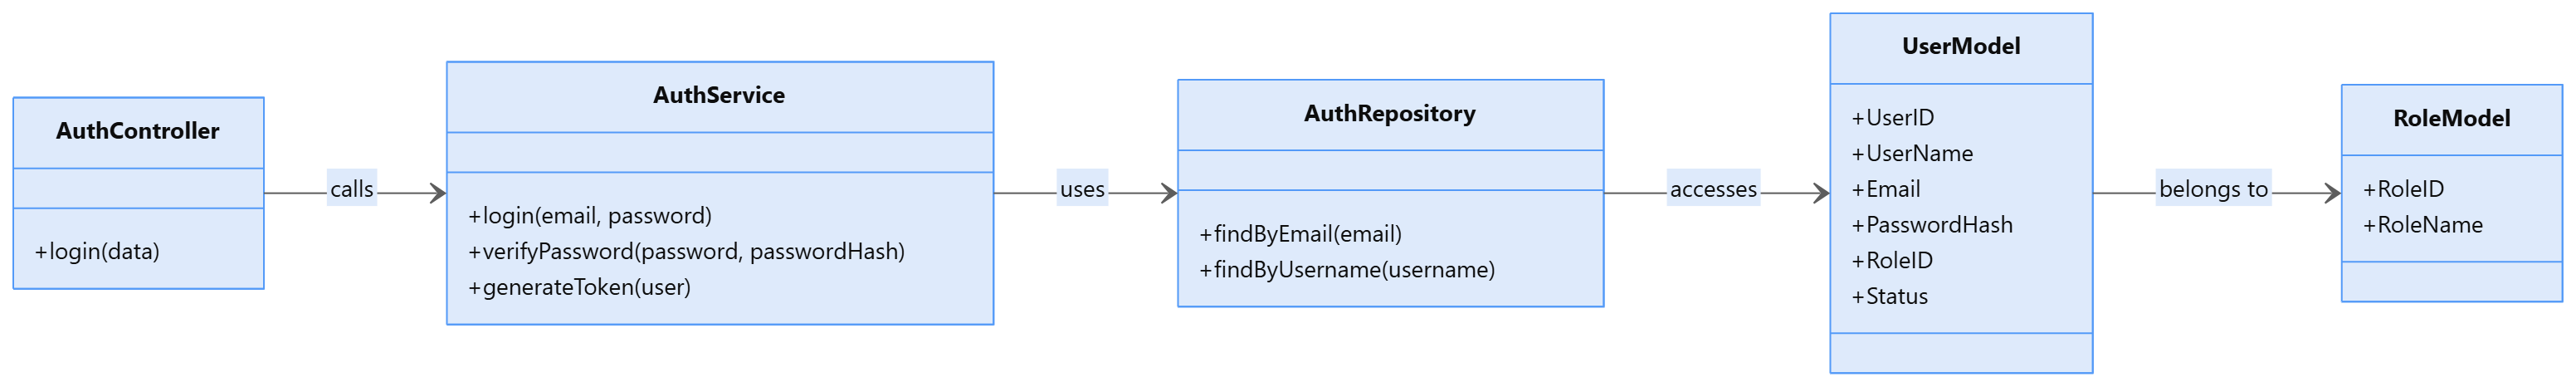
\includegraphics[width=1.1\textwidth]{images/14.png}
\end{figure}

\paragraph{Sequence Diagram}

\begin{figure}[H]
	\centering
	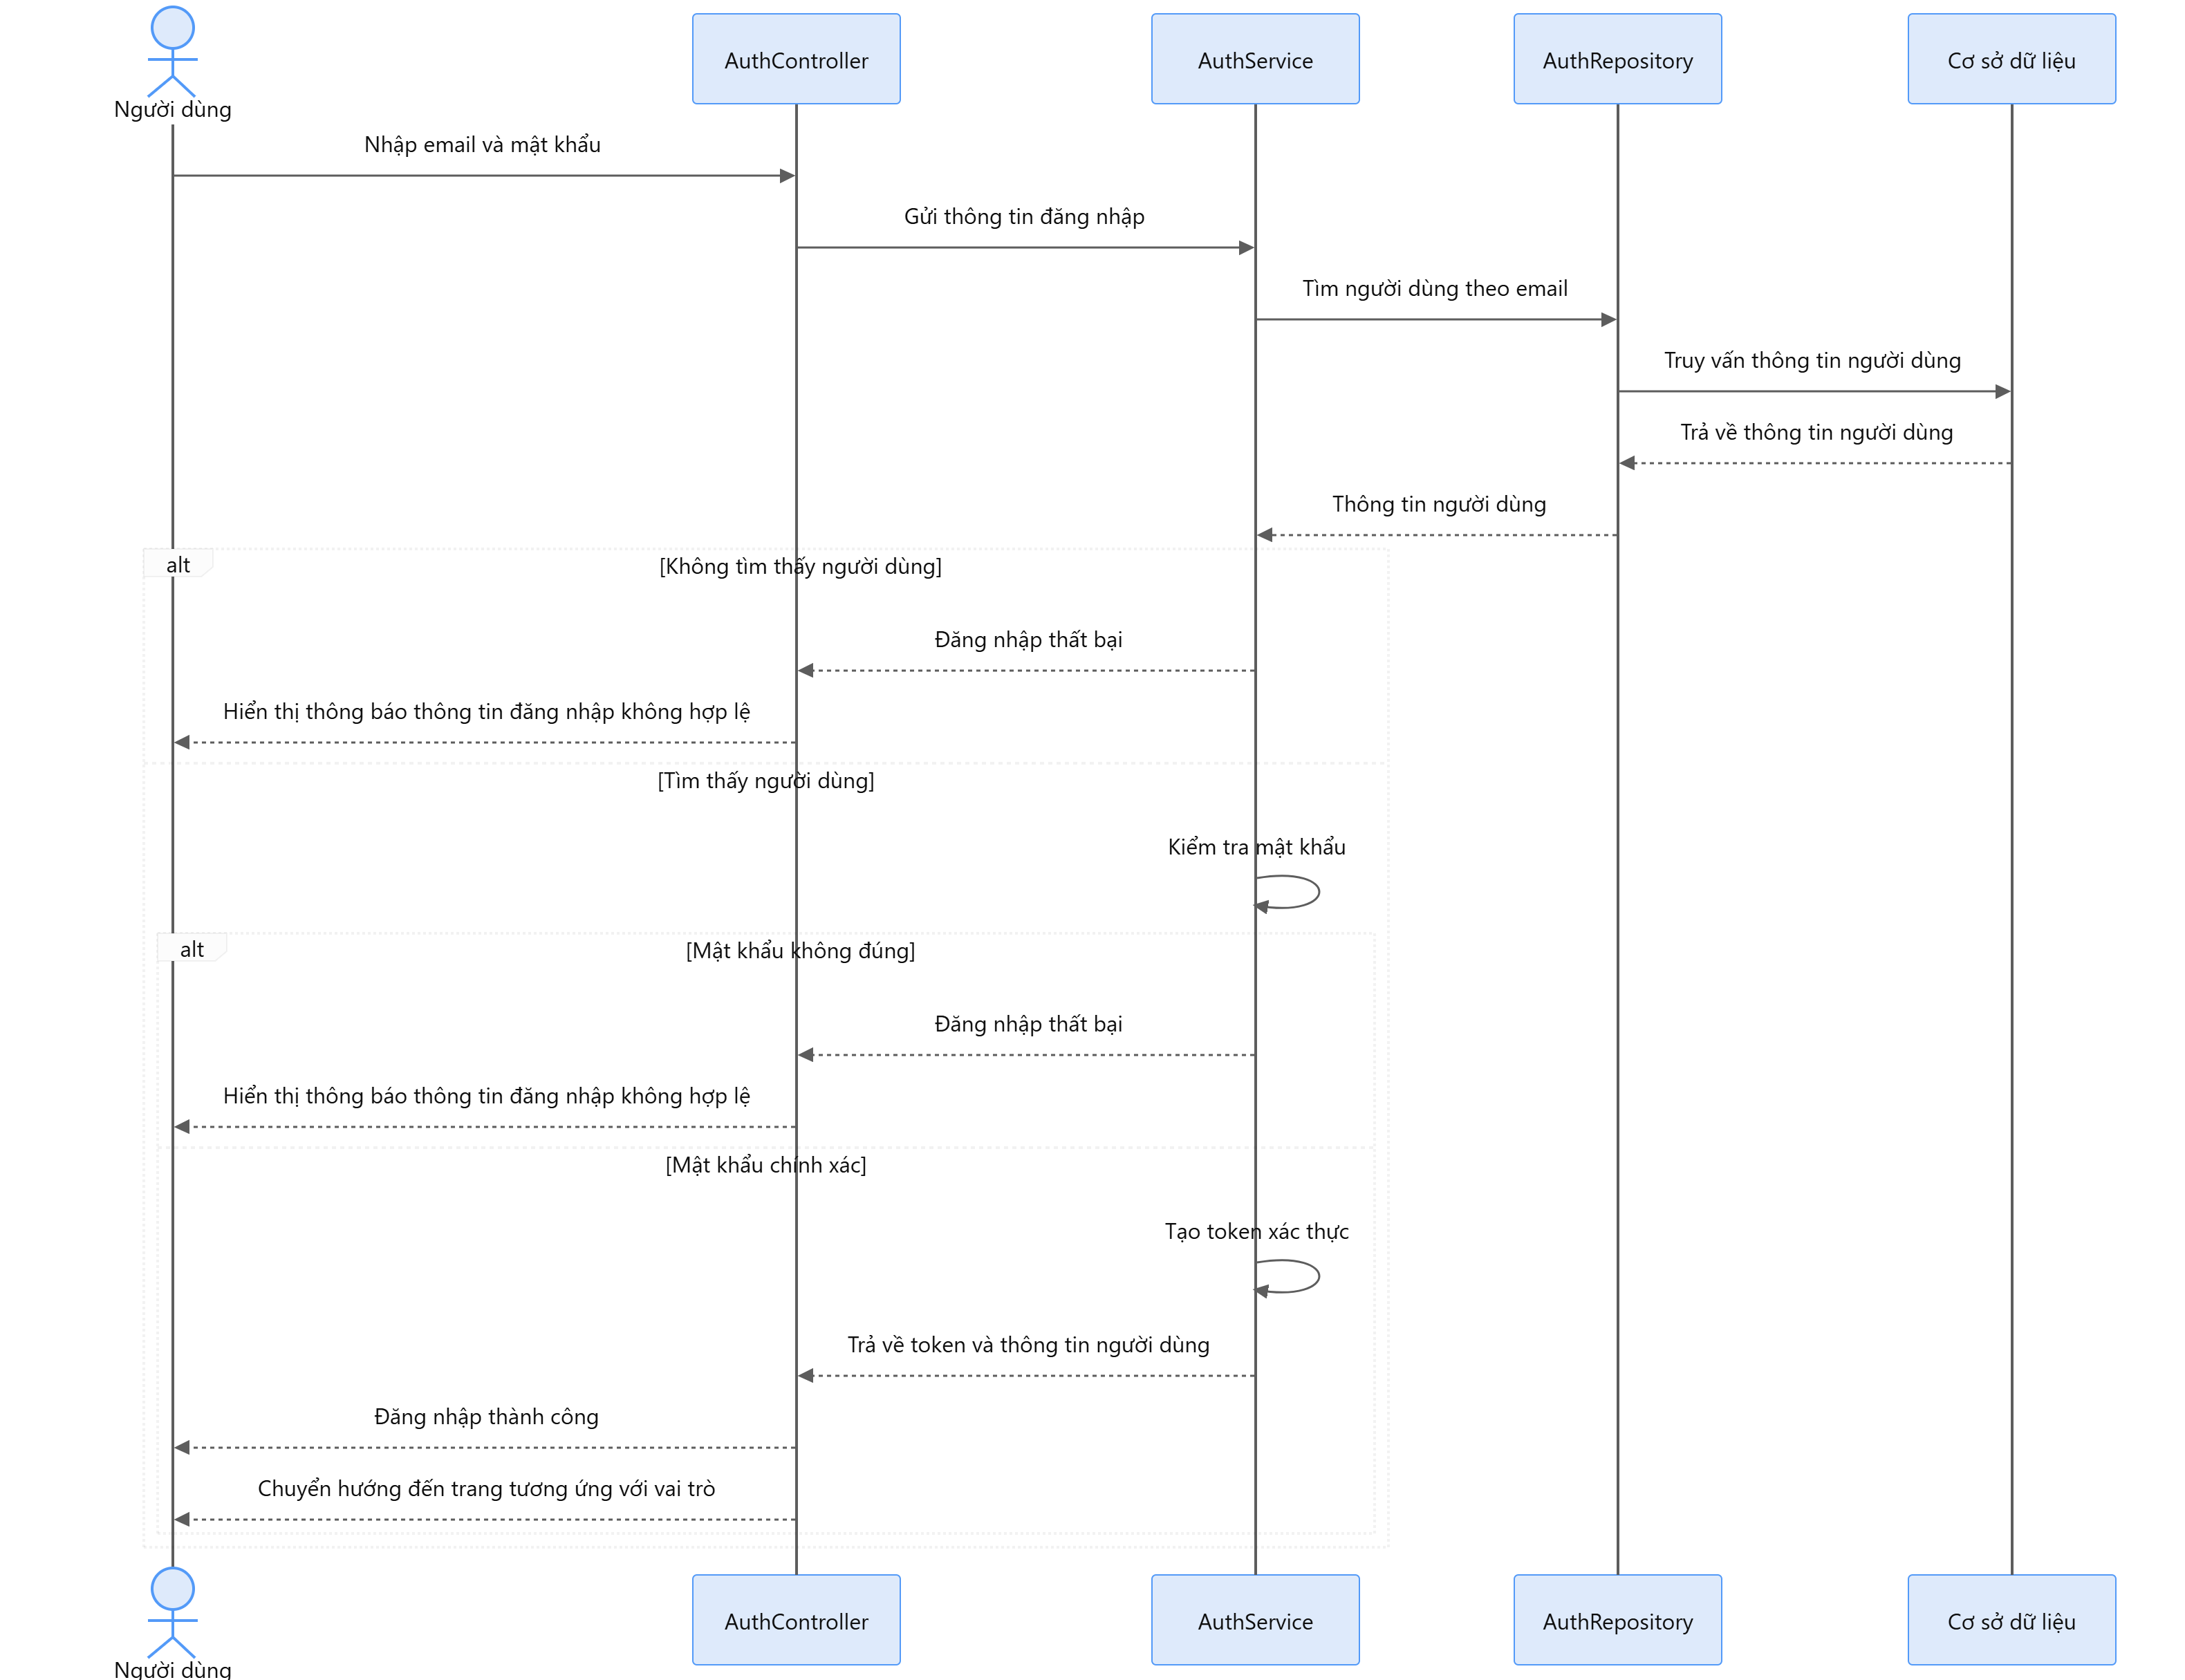
\includegraphics[width=1.1\textwidth]{images/15.png}
\end{figure}


\subsubsection{Quên mật khẩu}

\paragraph{Class Diagram}

\begin{figure}[H]
	\centering
	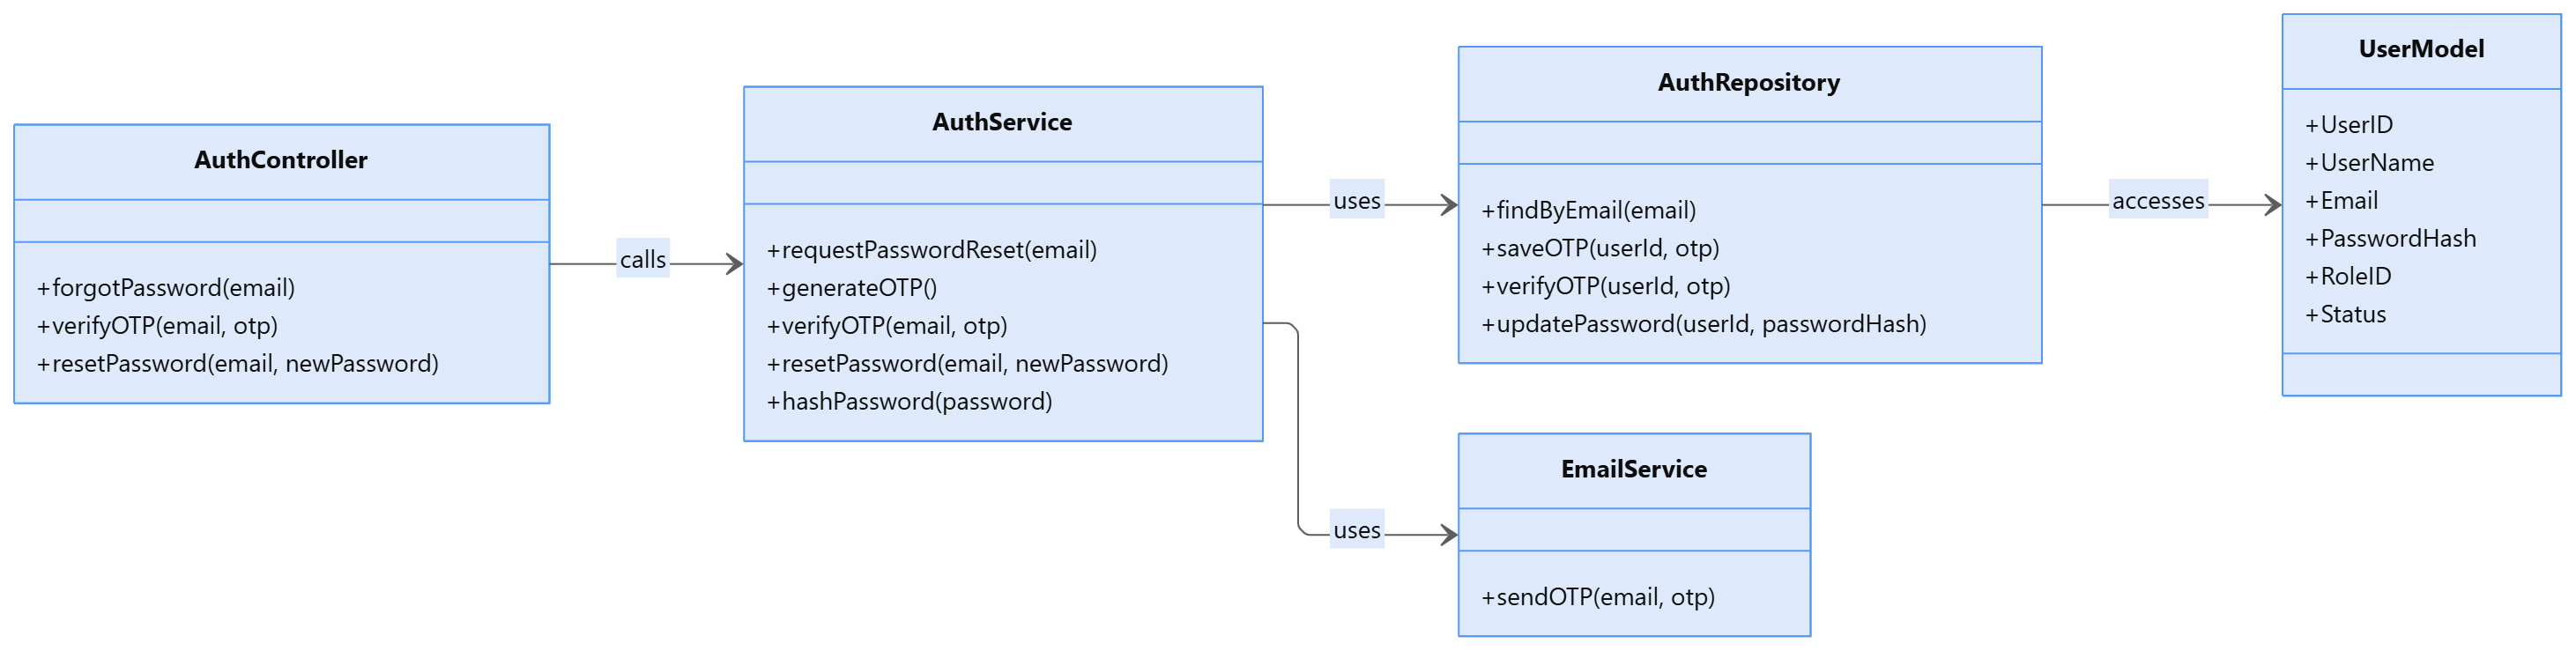
\includegraphics[width=1.1\textwidth]{images/16.png}
\end{figure}

\paragraph{Sequence Diagram}

\begin{figure}[H]
	\centering
	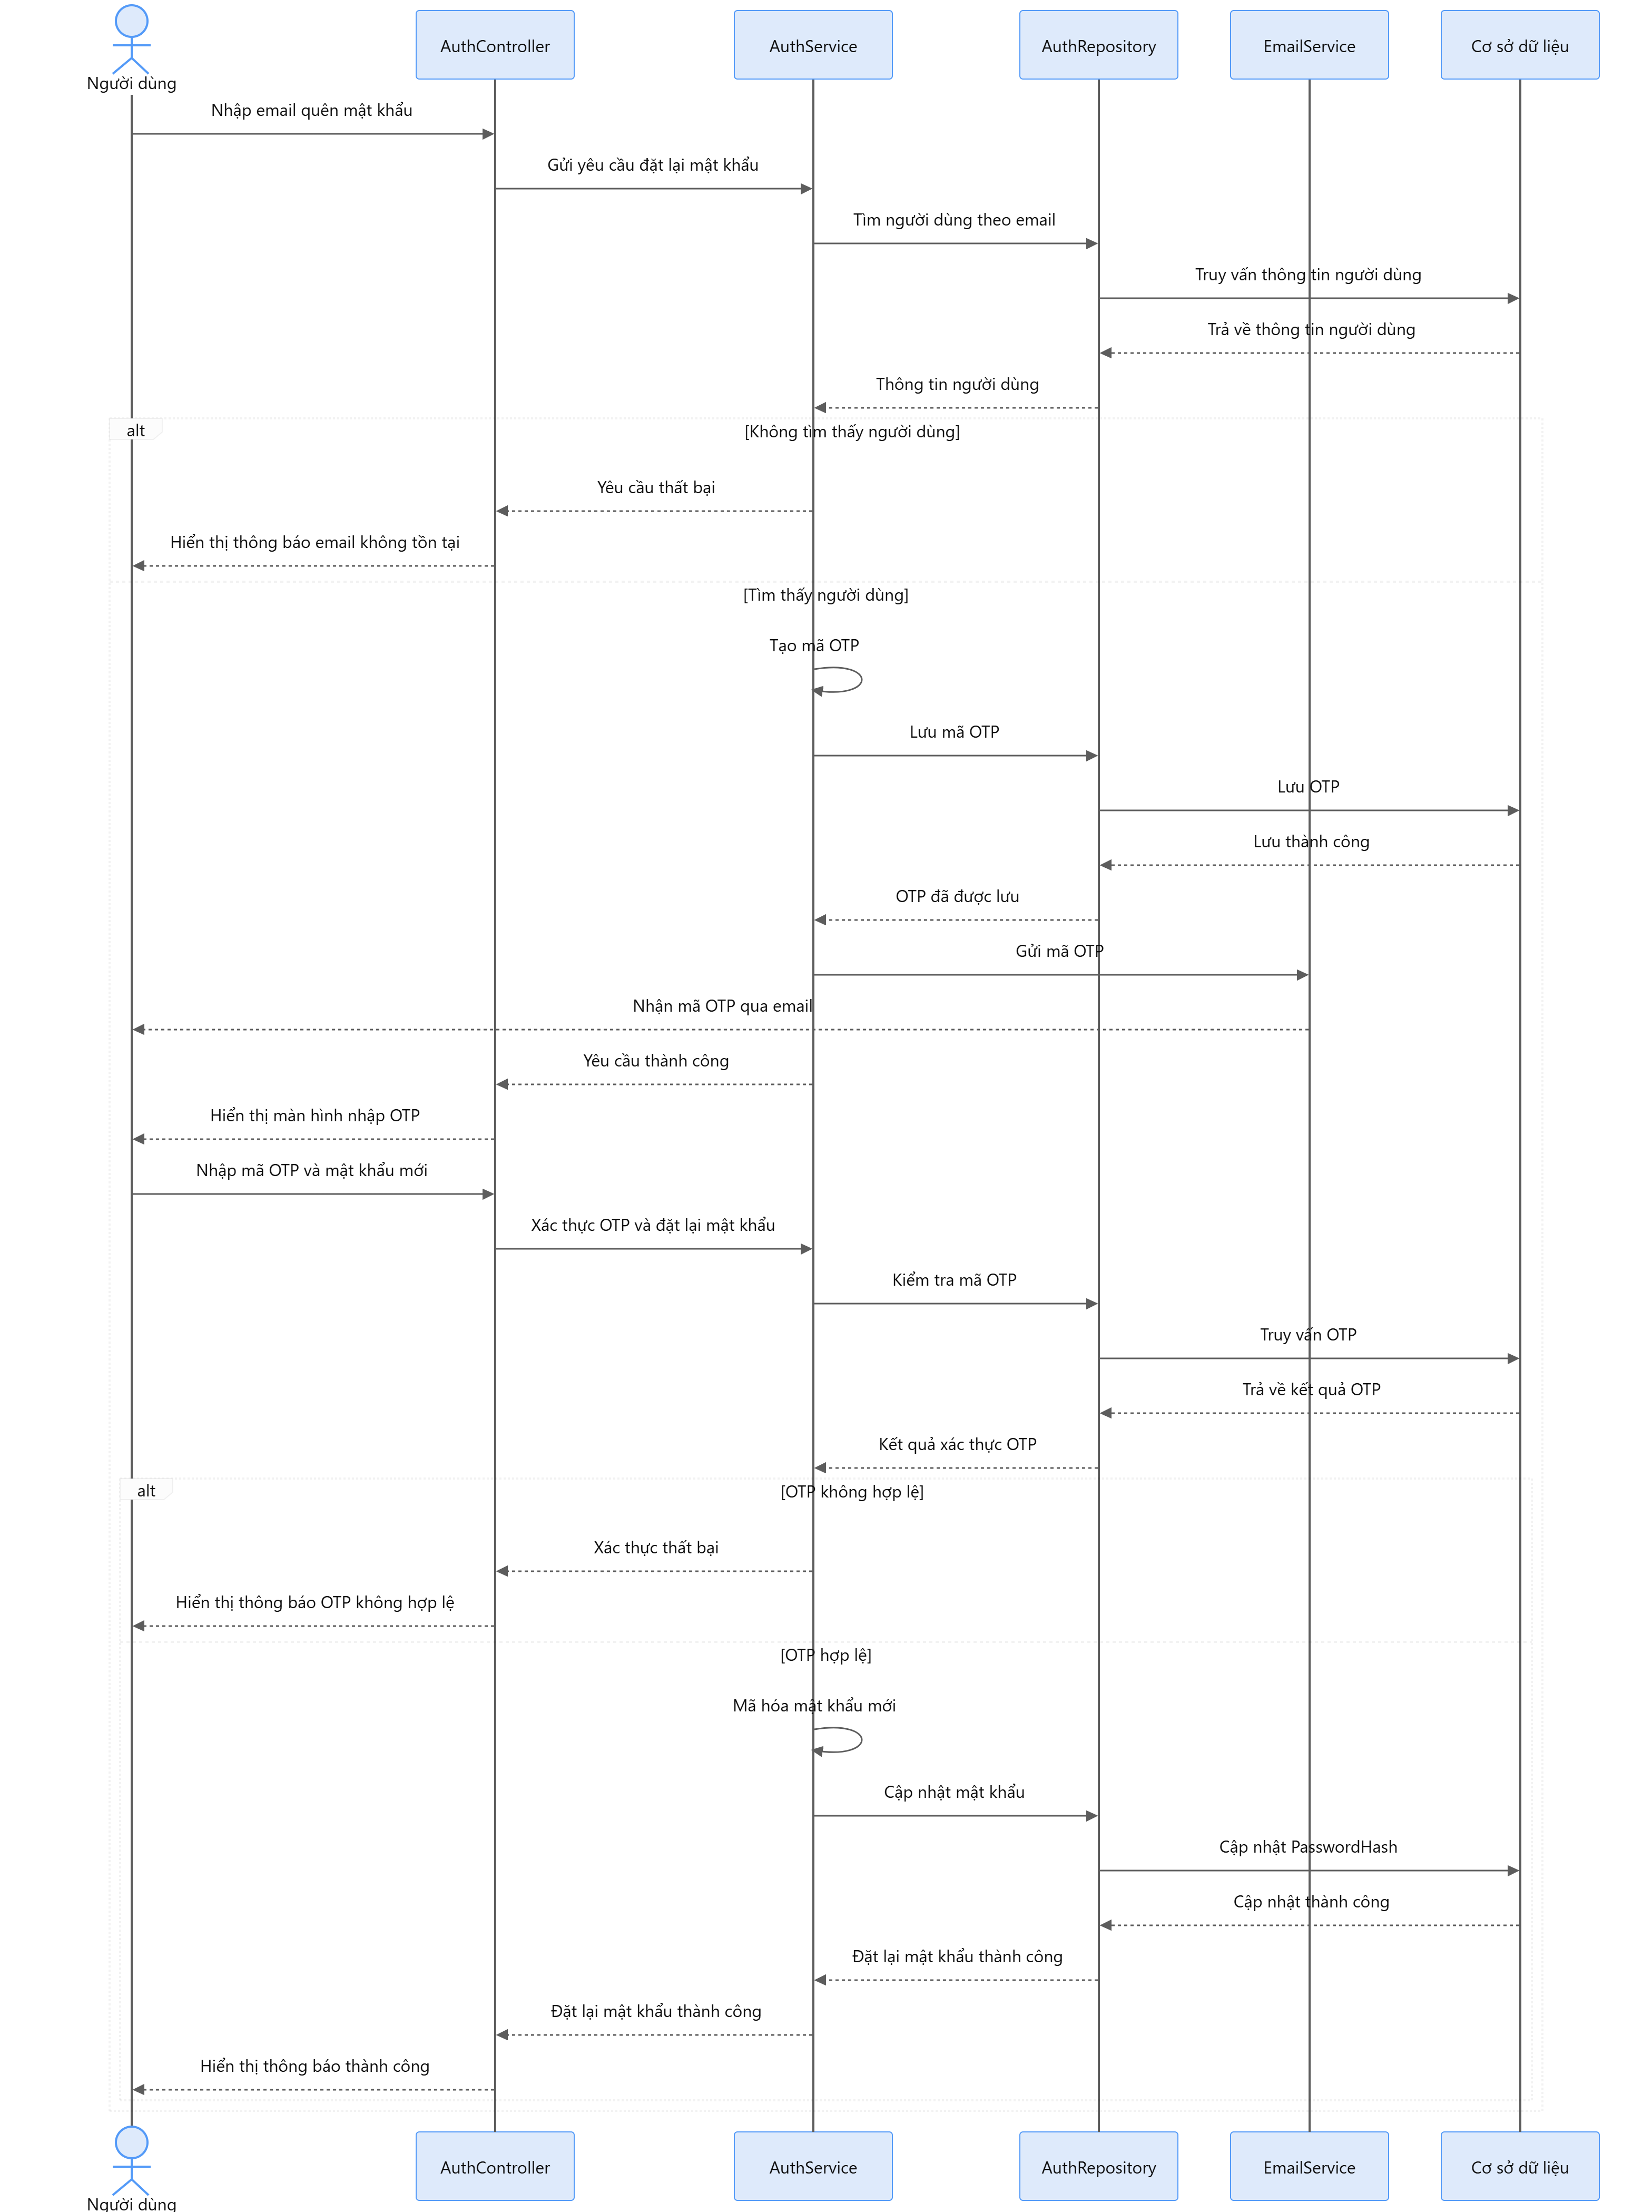
\includegraphics[width=1.1\textwidth]{images/17.png}
\end{figure}


\subsubsection{Đổi mật khẩu}

\paragraph{Class Diagram}

\begin{figure}[H]
	\centering
	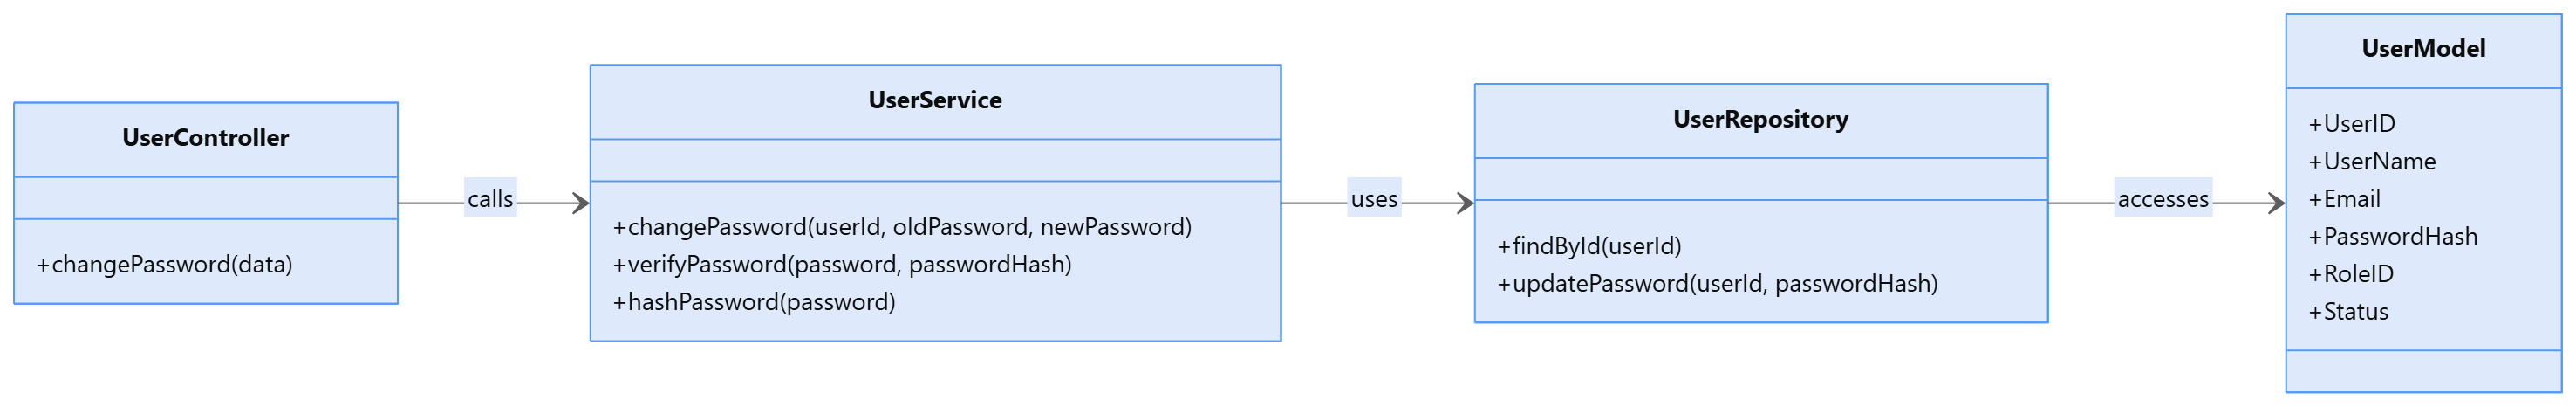
\includegraphics[width=1.1\textwidth]{images/18.png}
\end{figure}

\paragraph{Sequence Diagram}

\begin{figure}[H]
	\centering
	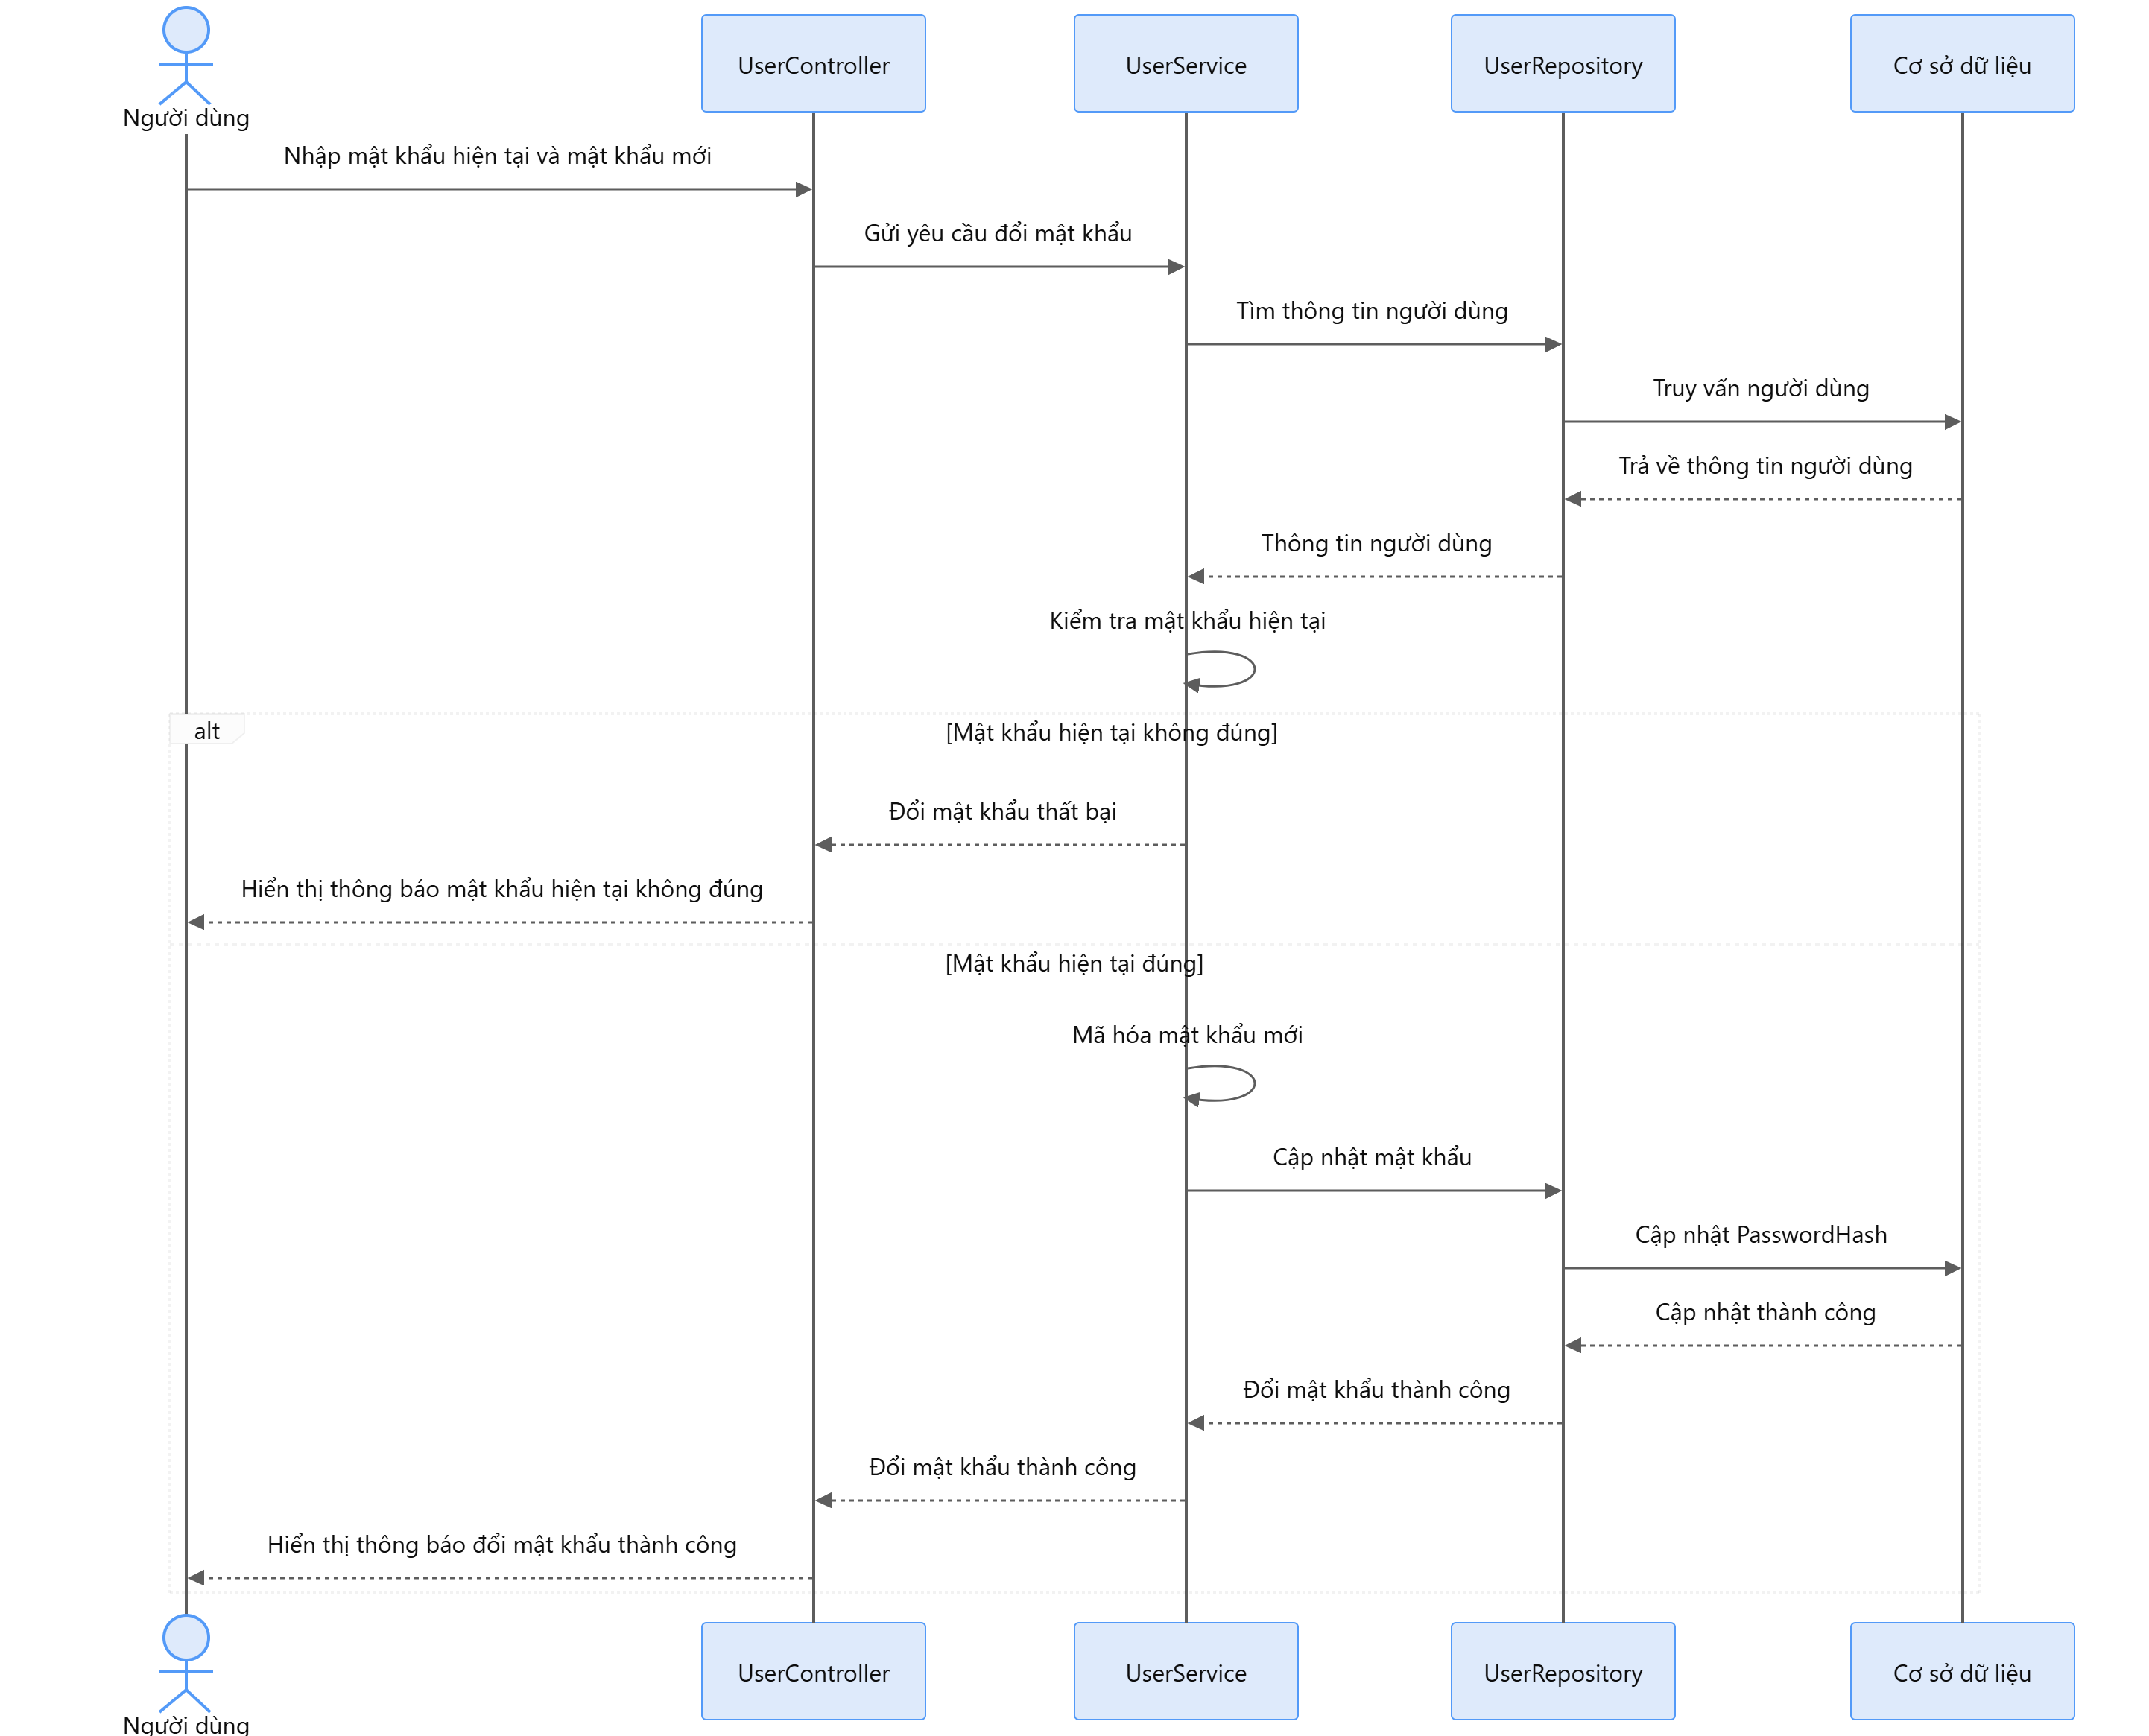
\includegraphics[width=1.1\textwidth]{images/19.png}
\end{figure}


% =========================================================
% 3.2 Photographer Management Module
% =========================================================

\subsection{Photographer Management Module}

\subsubsection{Quản lý hồ sơ}

\paragraph{Class Diagram}

\begin{figure}[H]
	\centering
	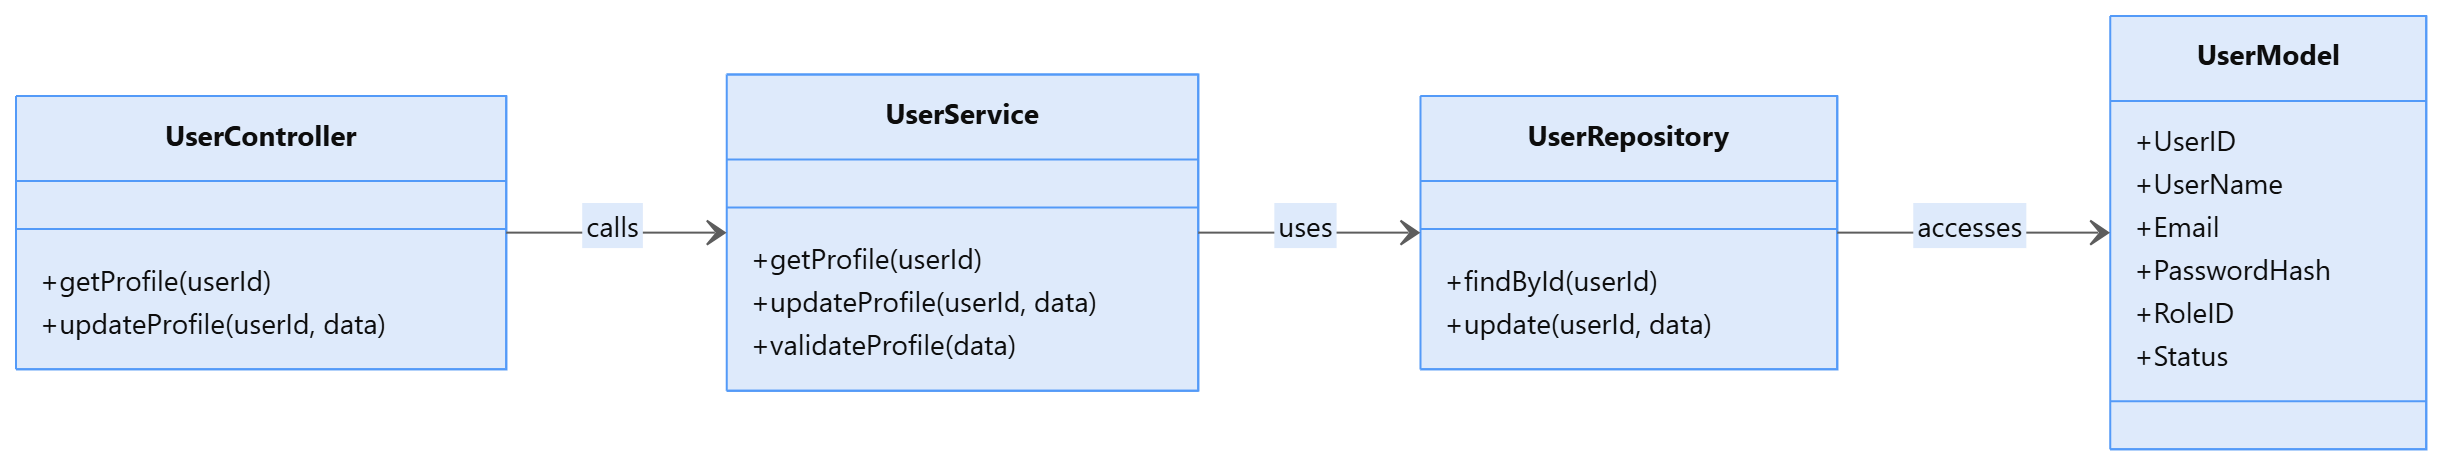
\includegraphics[width=1.1\textwidth]{images/20.png}
\end{figure}

\paragraph{Sequence Diagram}

\begin{figure}[H]
	\centering
	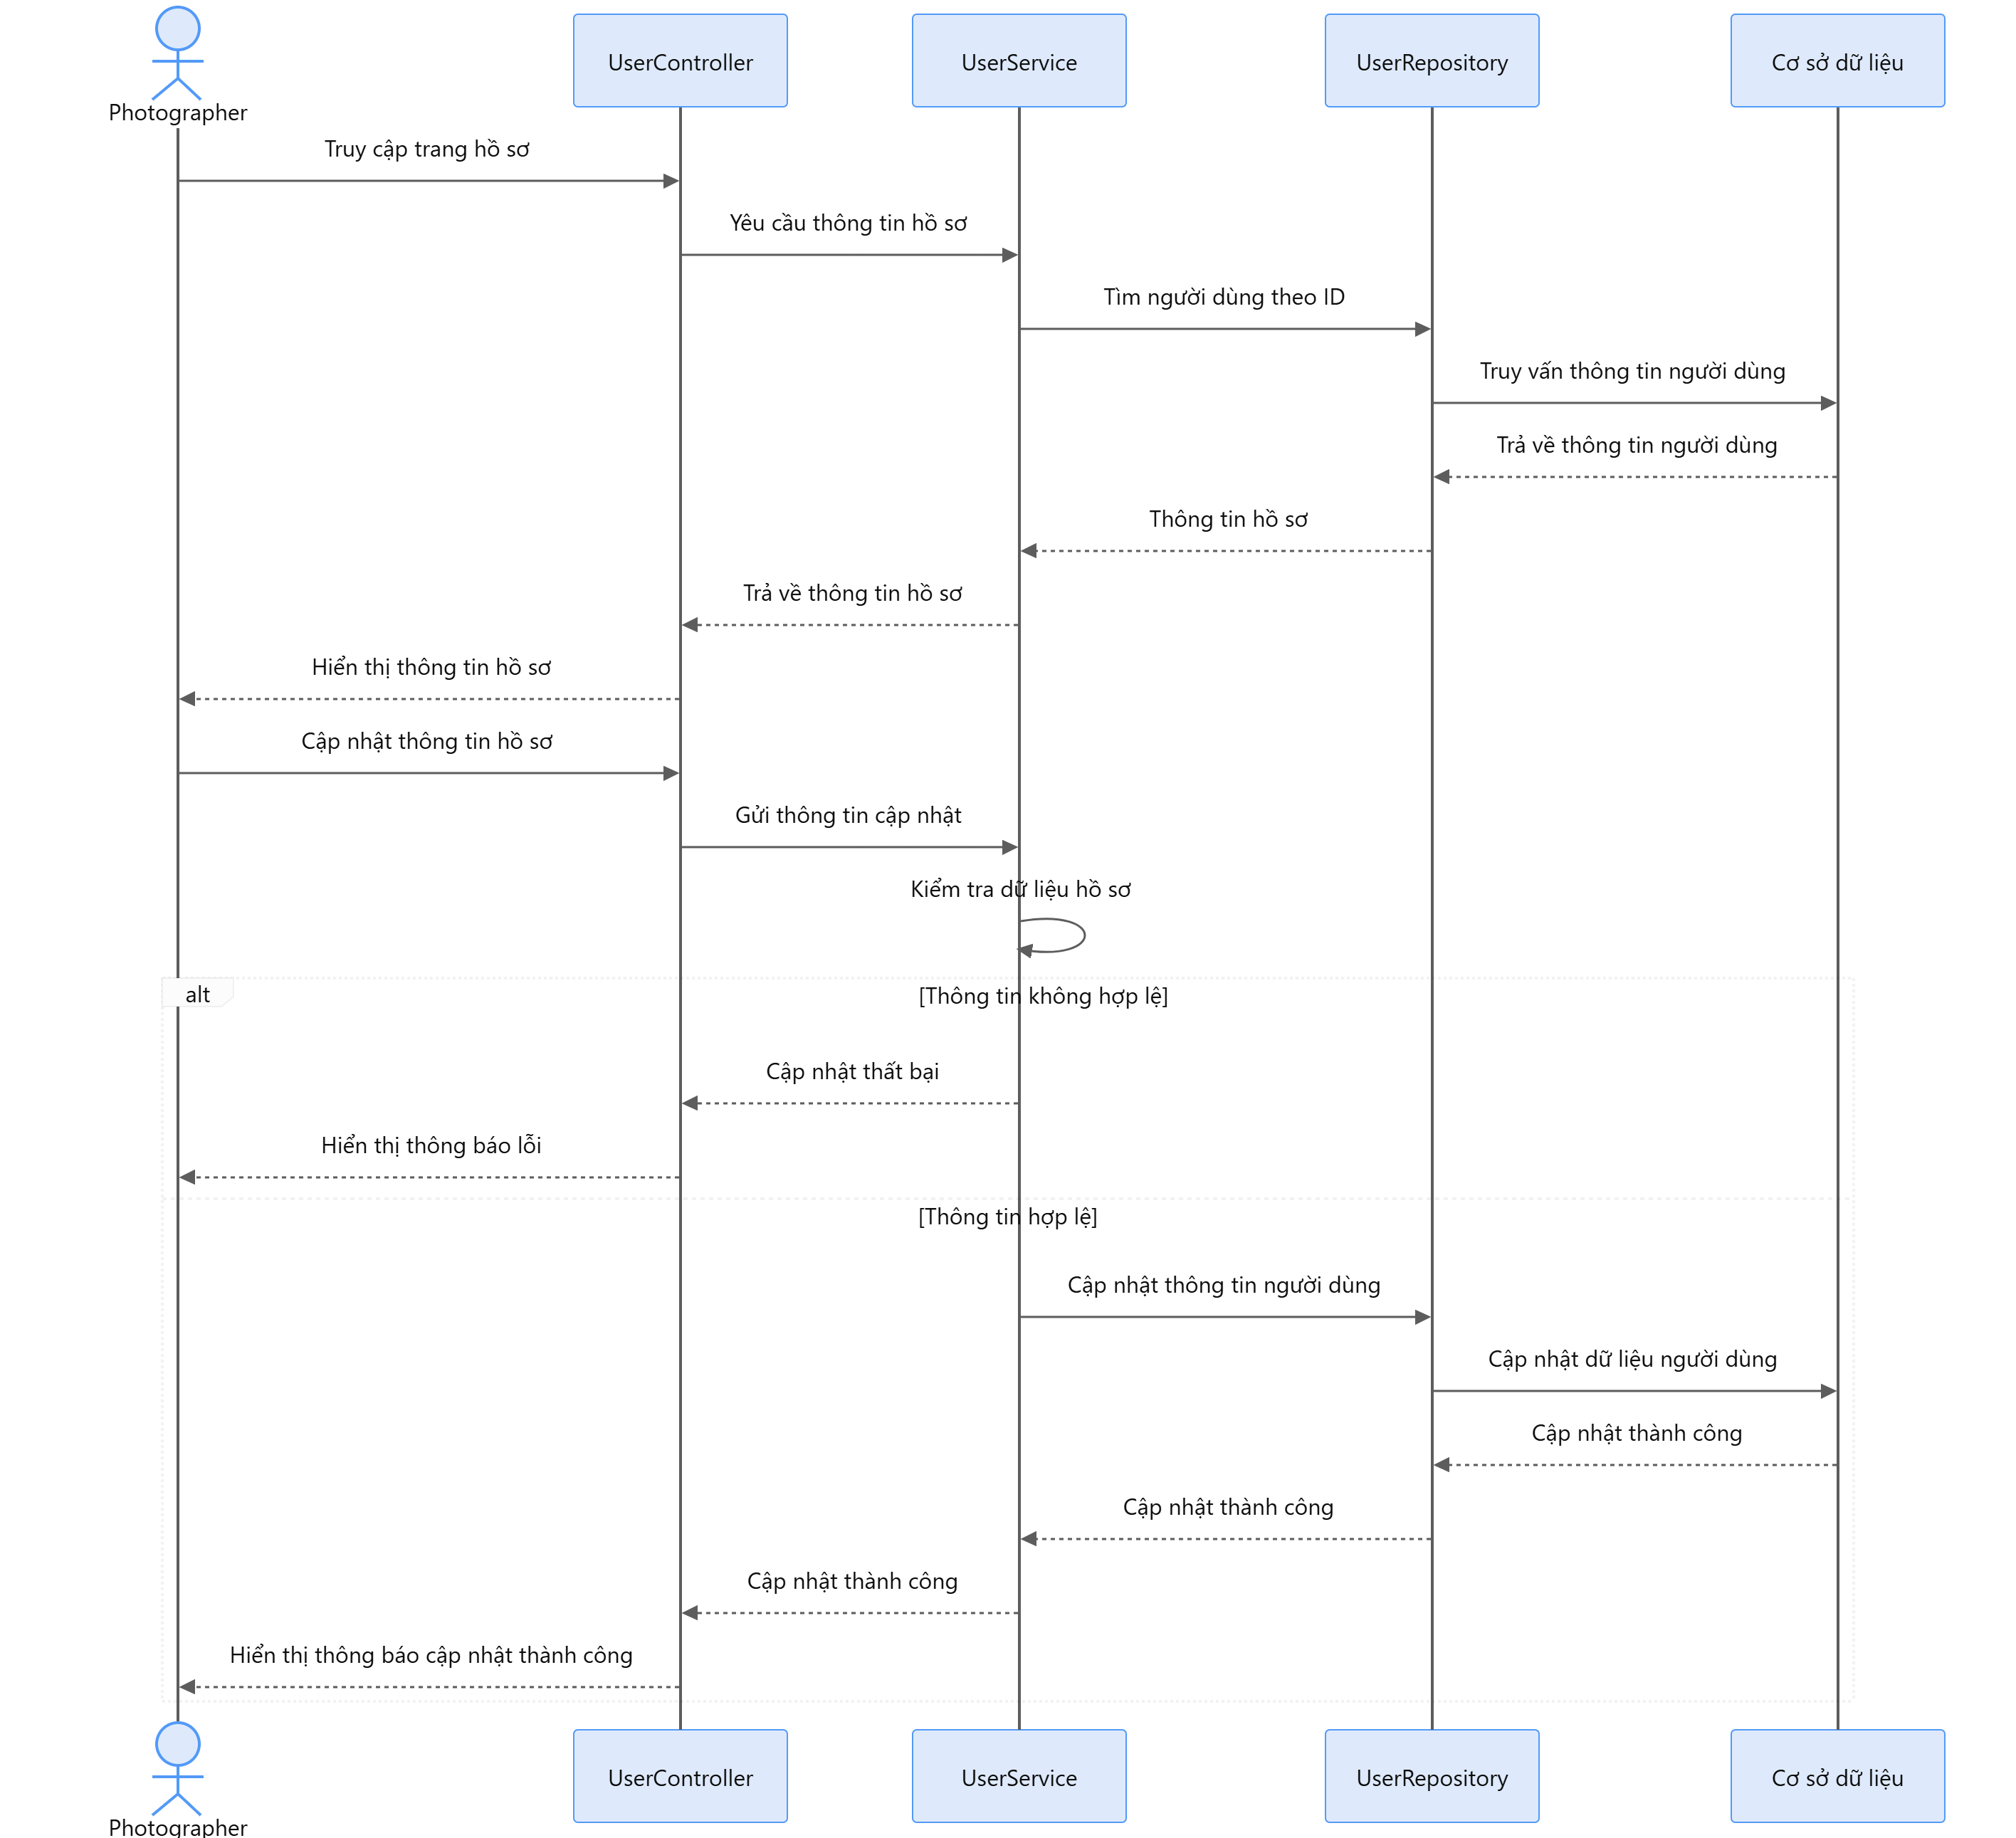
\includegraphics[width=1.1\textwidth]{images/21.png}
\end{figure}


% =========================================================
% 3.3 Service Search and Discovery Module
% =========================================================

\subsection{Service Search and Discovery Module}

\subsubsection{Tìm kiếm Creative Space}

\paragraph{Class Diagram}

\begin{figure}[H]
	\centering
	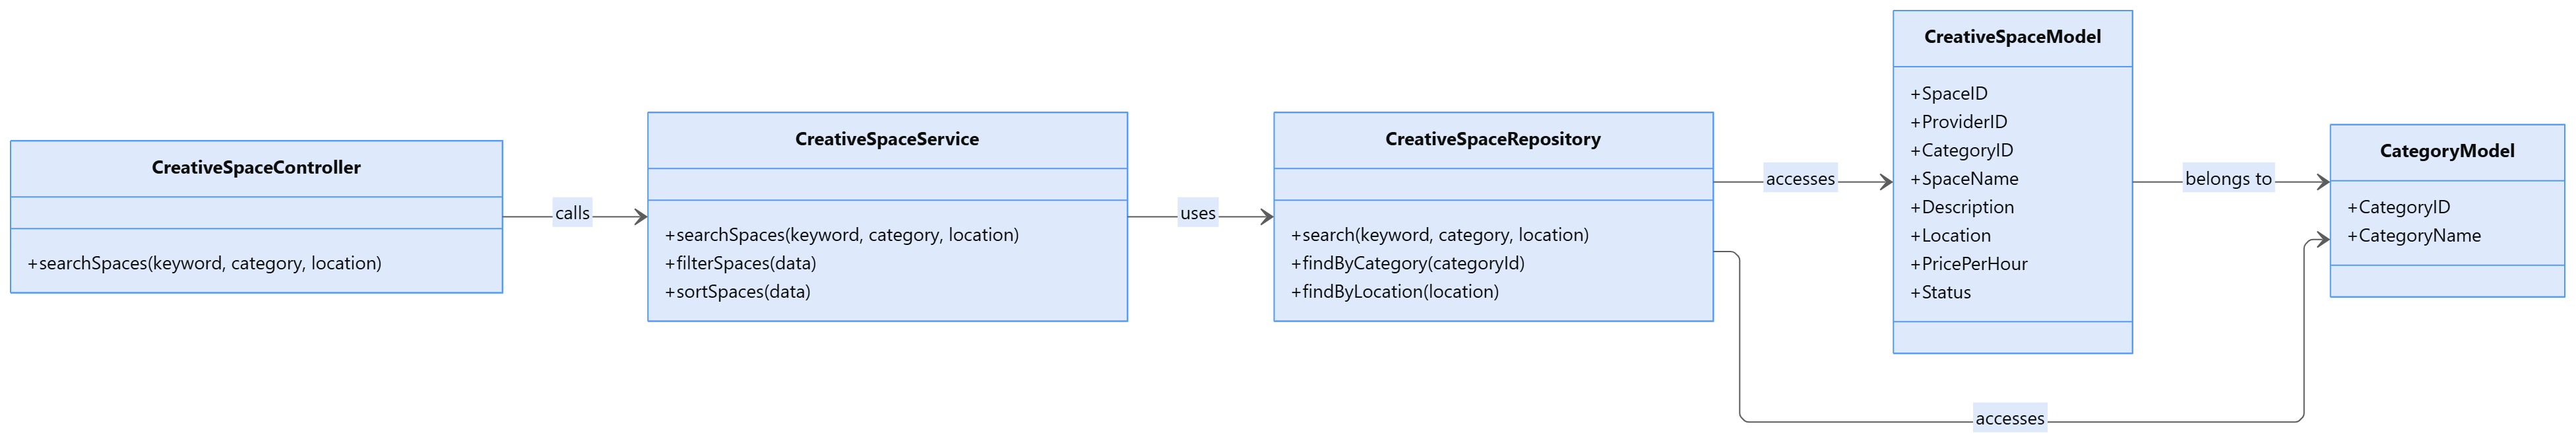
\includegraphics[width=1.1\textwidth]{images/22.png}
\end{figure}

\paragraph{Sequence Diagram}

\begin{figure}[H]
	\centering
	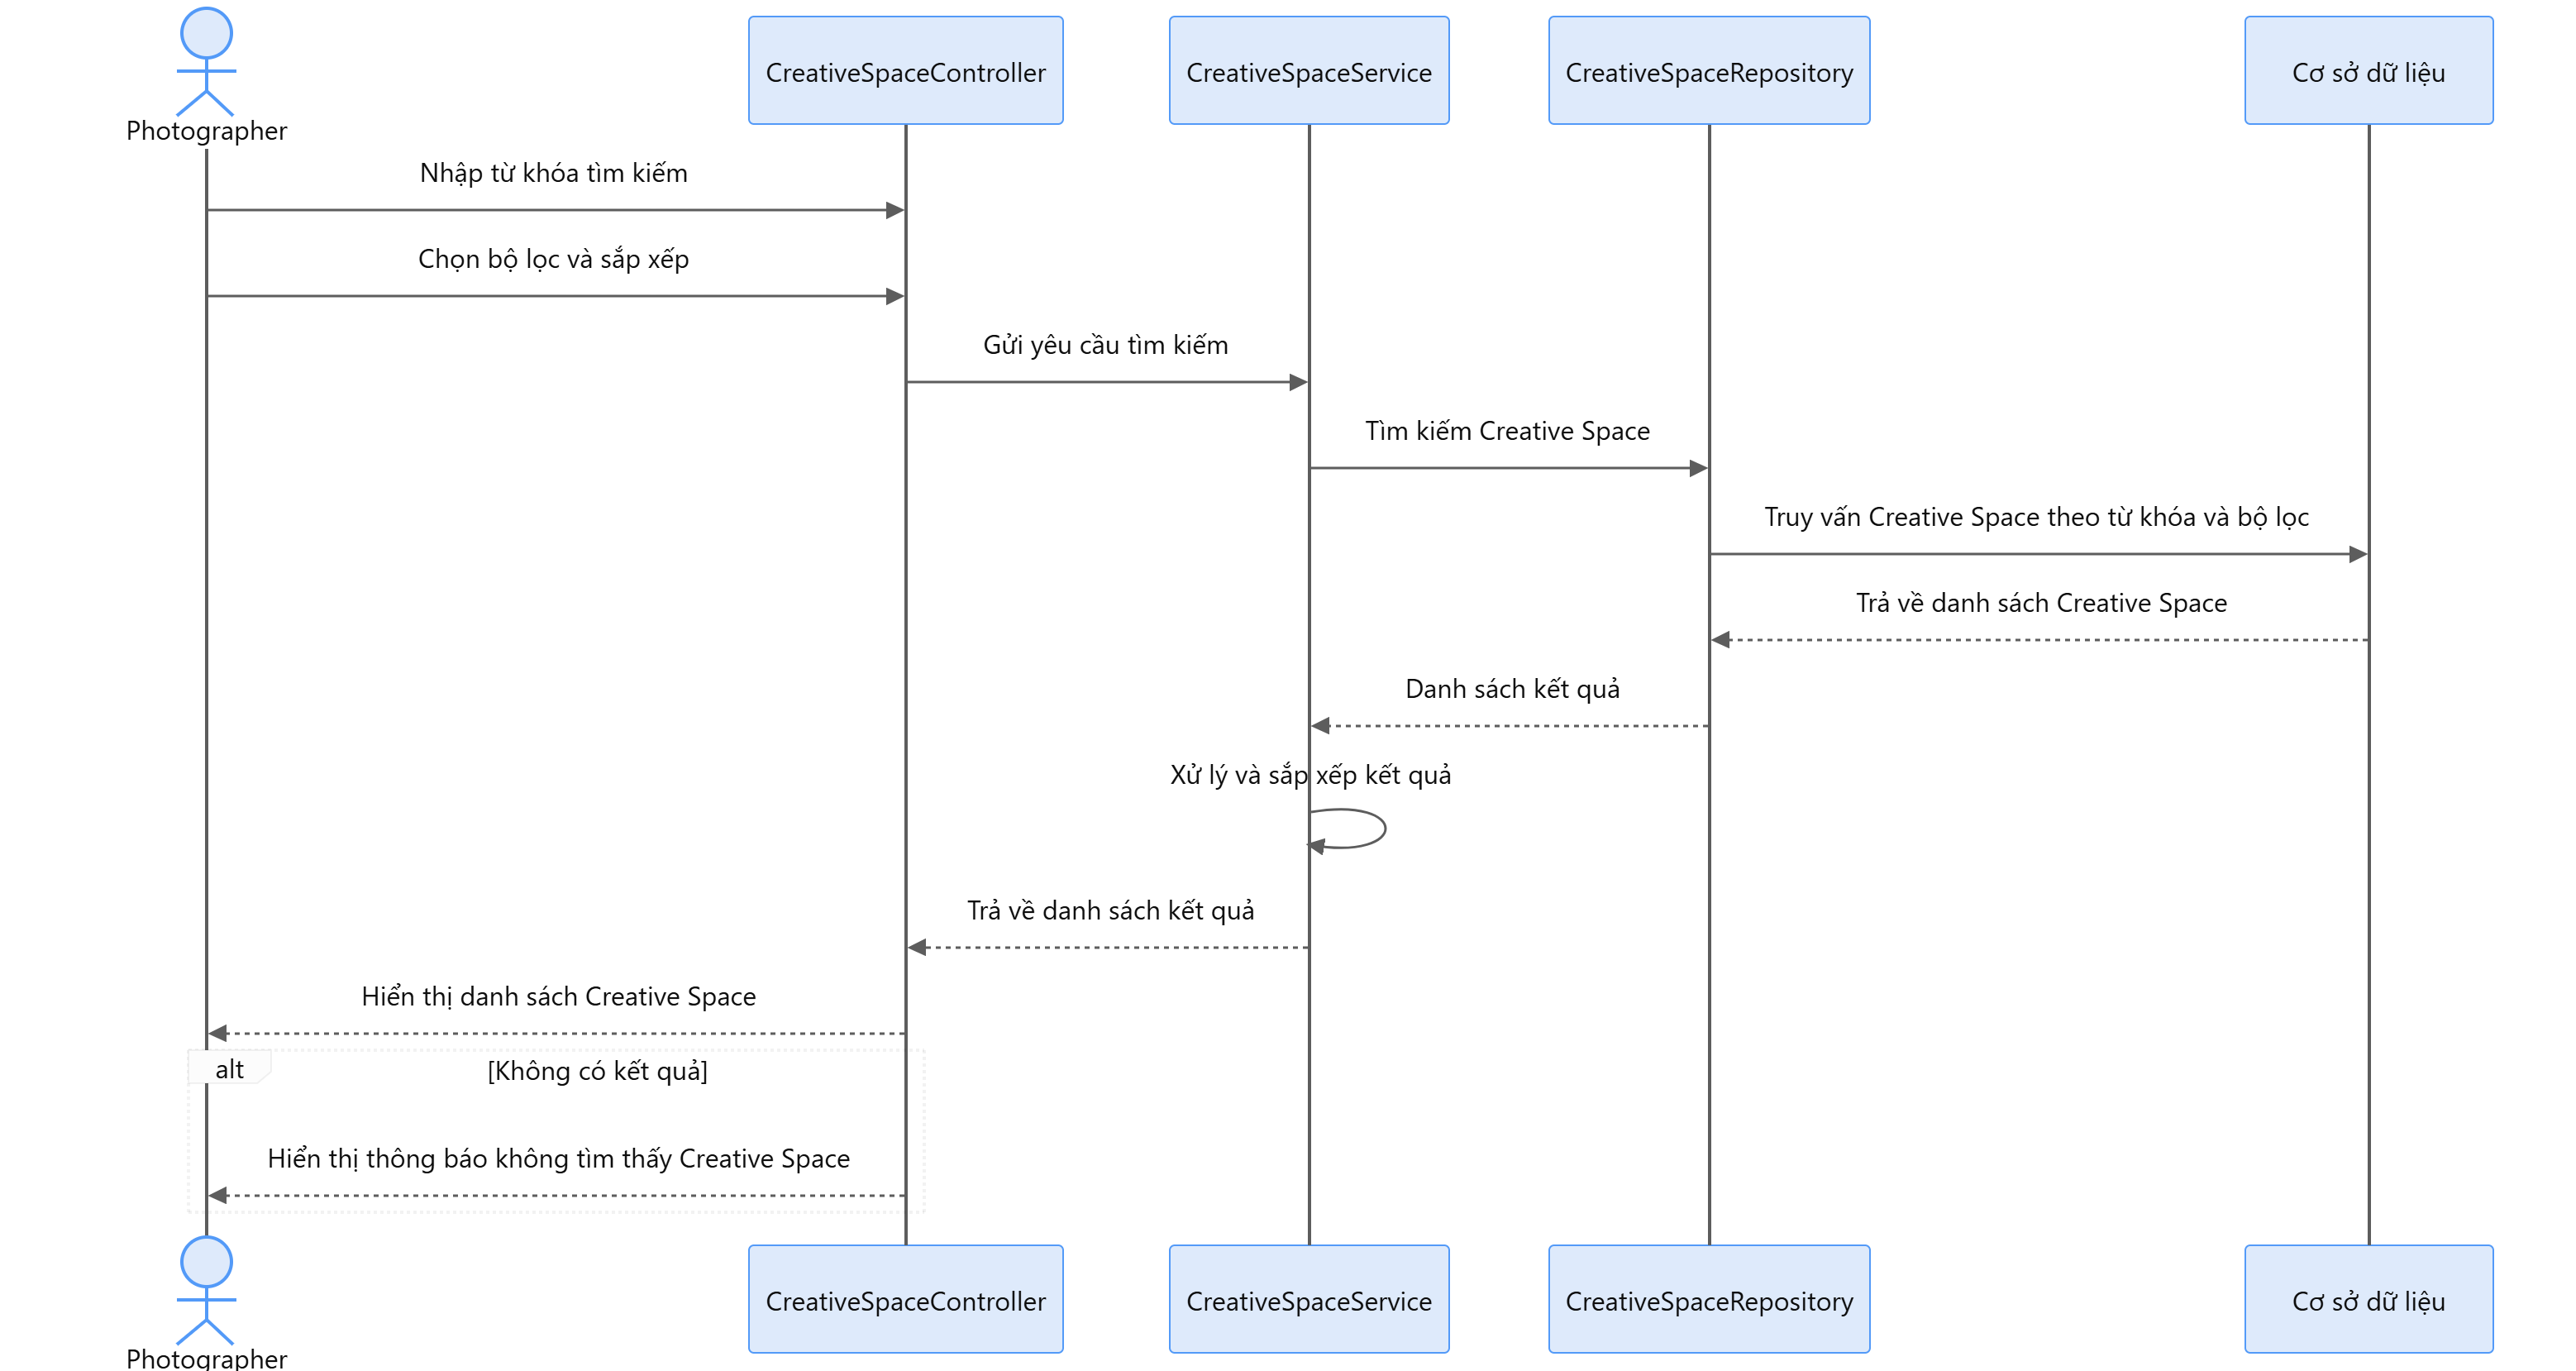
\includegraphics[width=1.1\textwidth]{images/23.png}
\end{figure}


\subsubsection{Xem chi tiết Creative Space}

\paragraph{Class Diagram}

\begin{figure}[H]
	\centering
	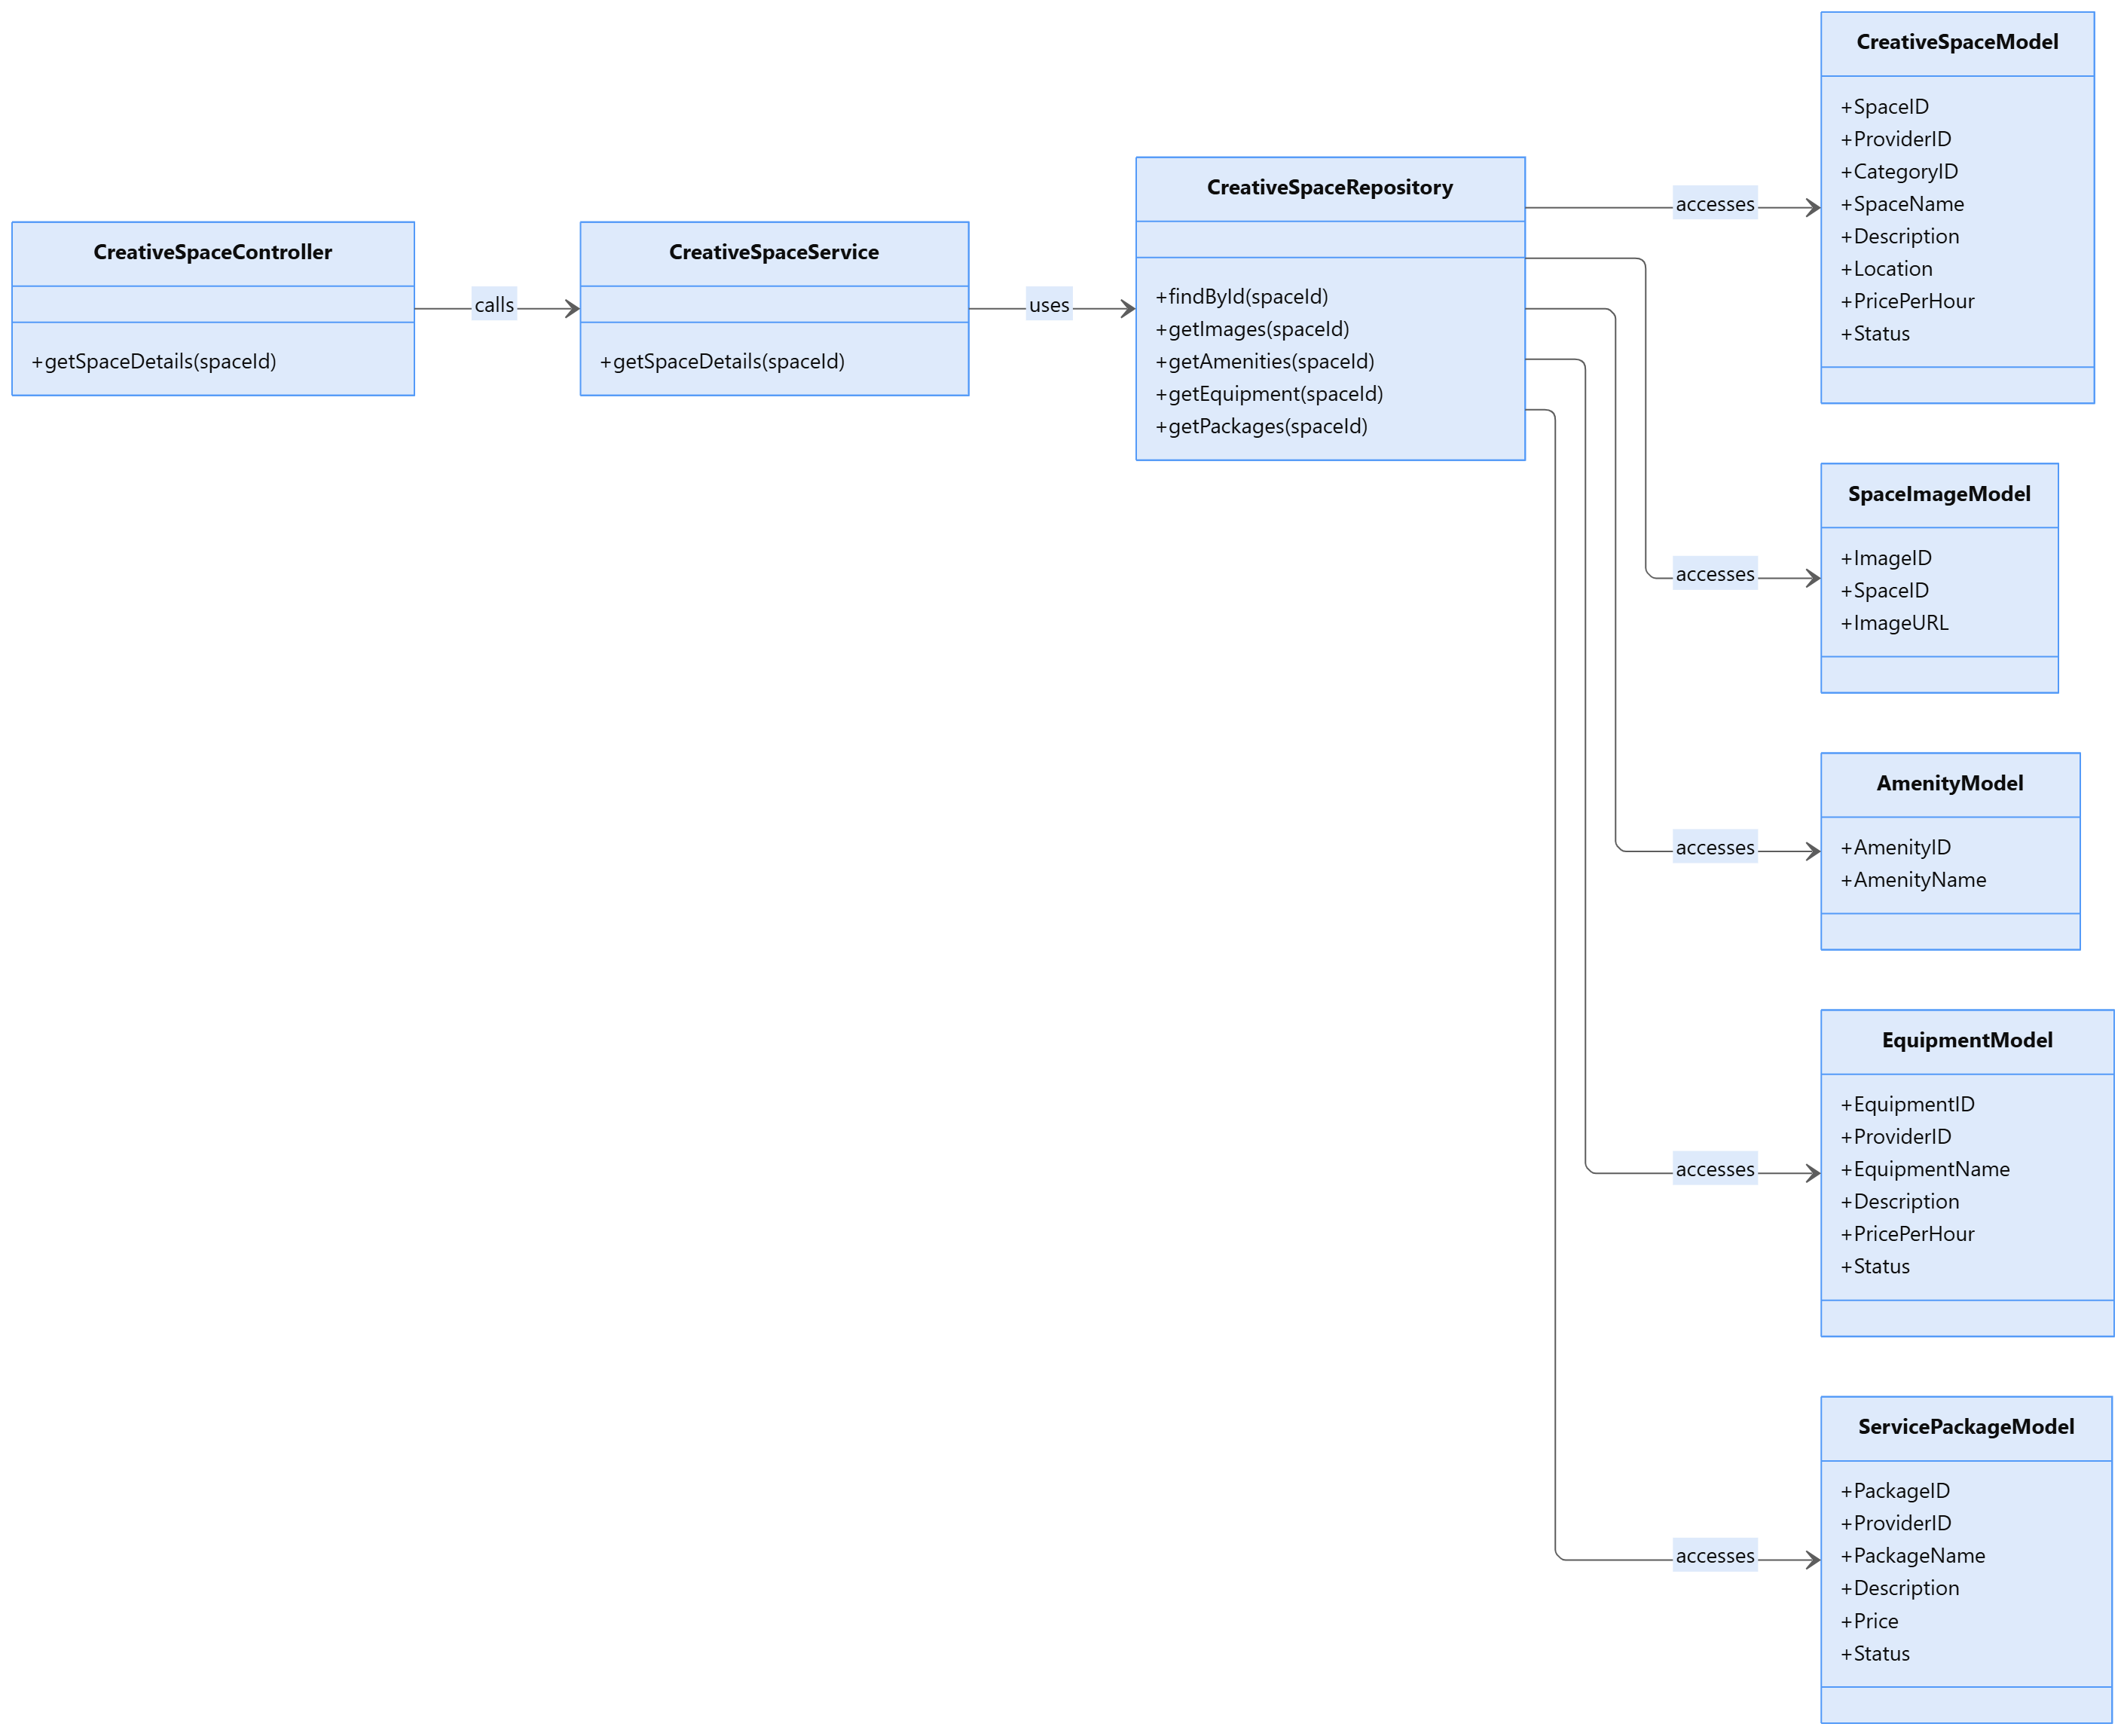
\includegraphics[width=1.1\textwidth]{images/24.png}
\end{figure}

\paragraph{Sequence Diagram}

\begin{figure}[H]
	\centering
	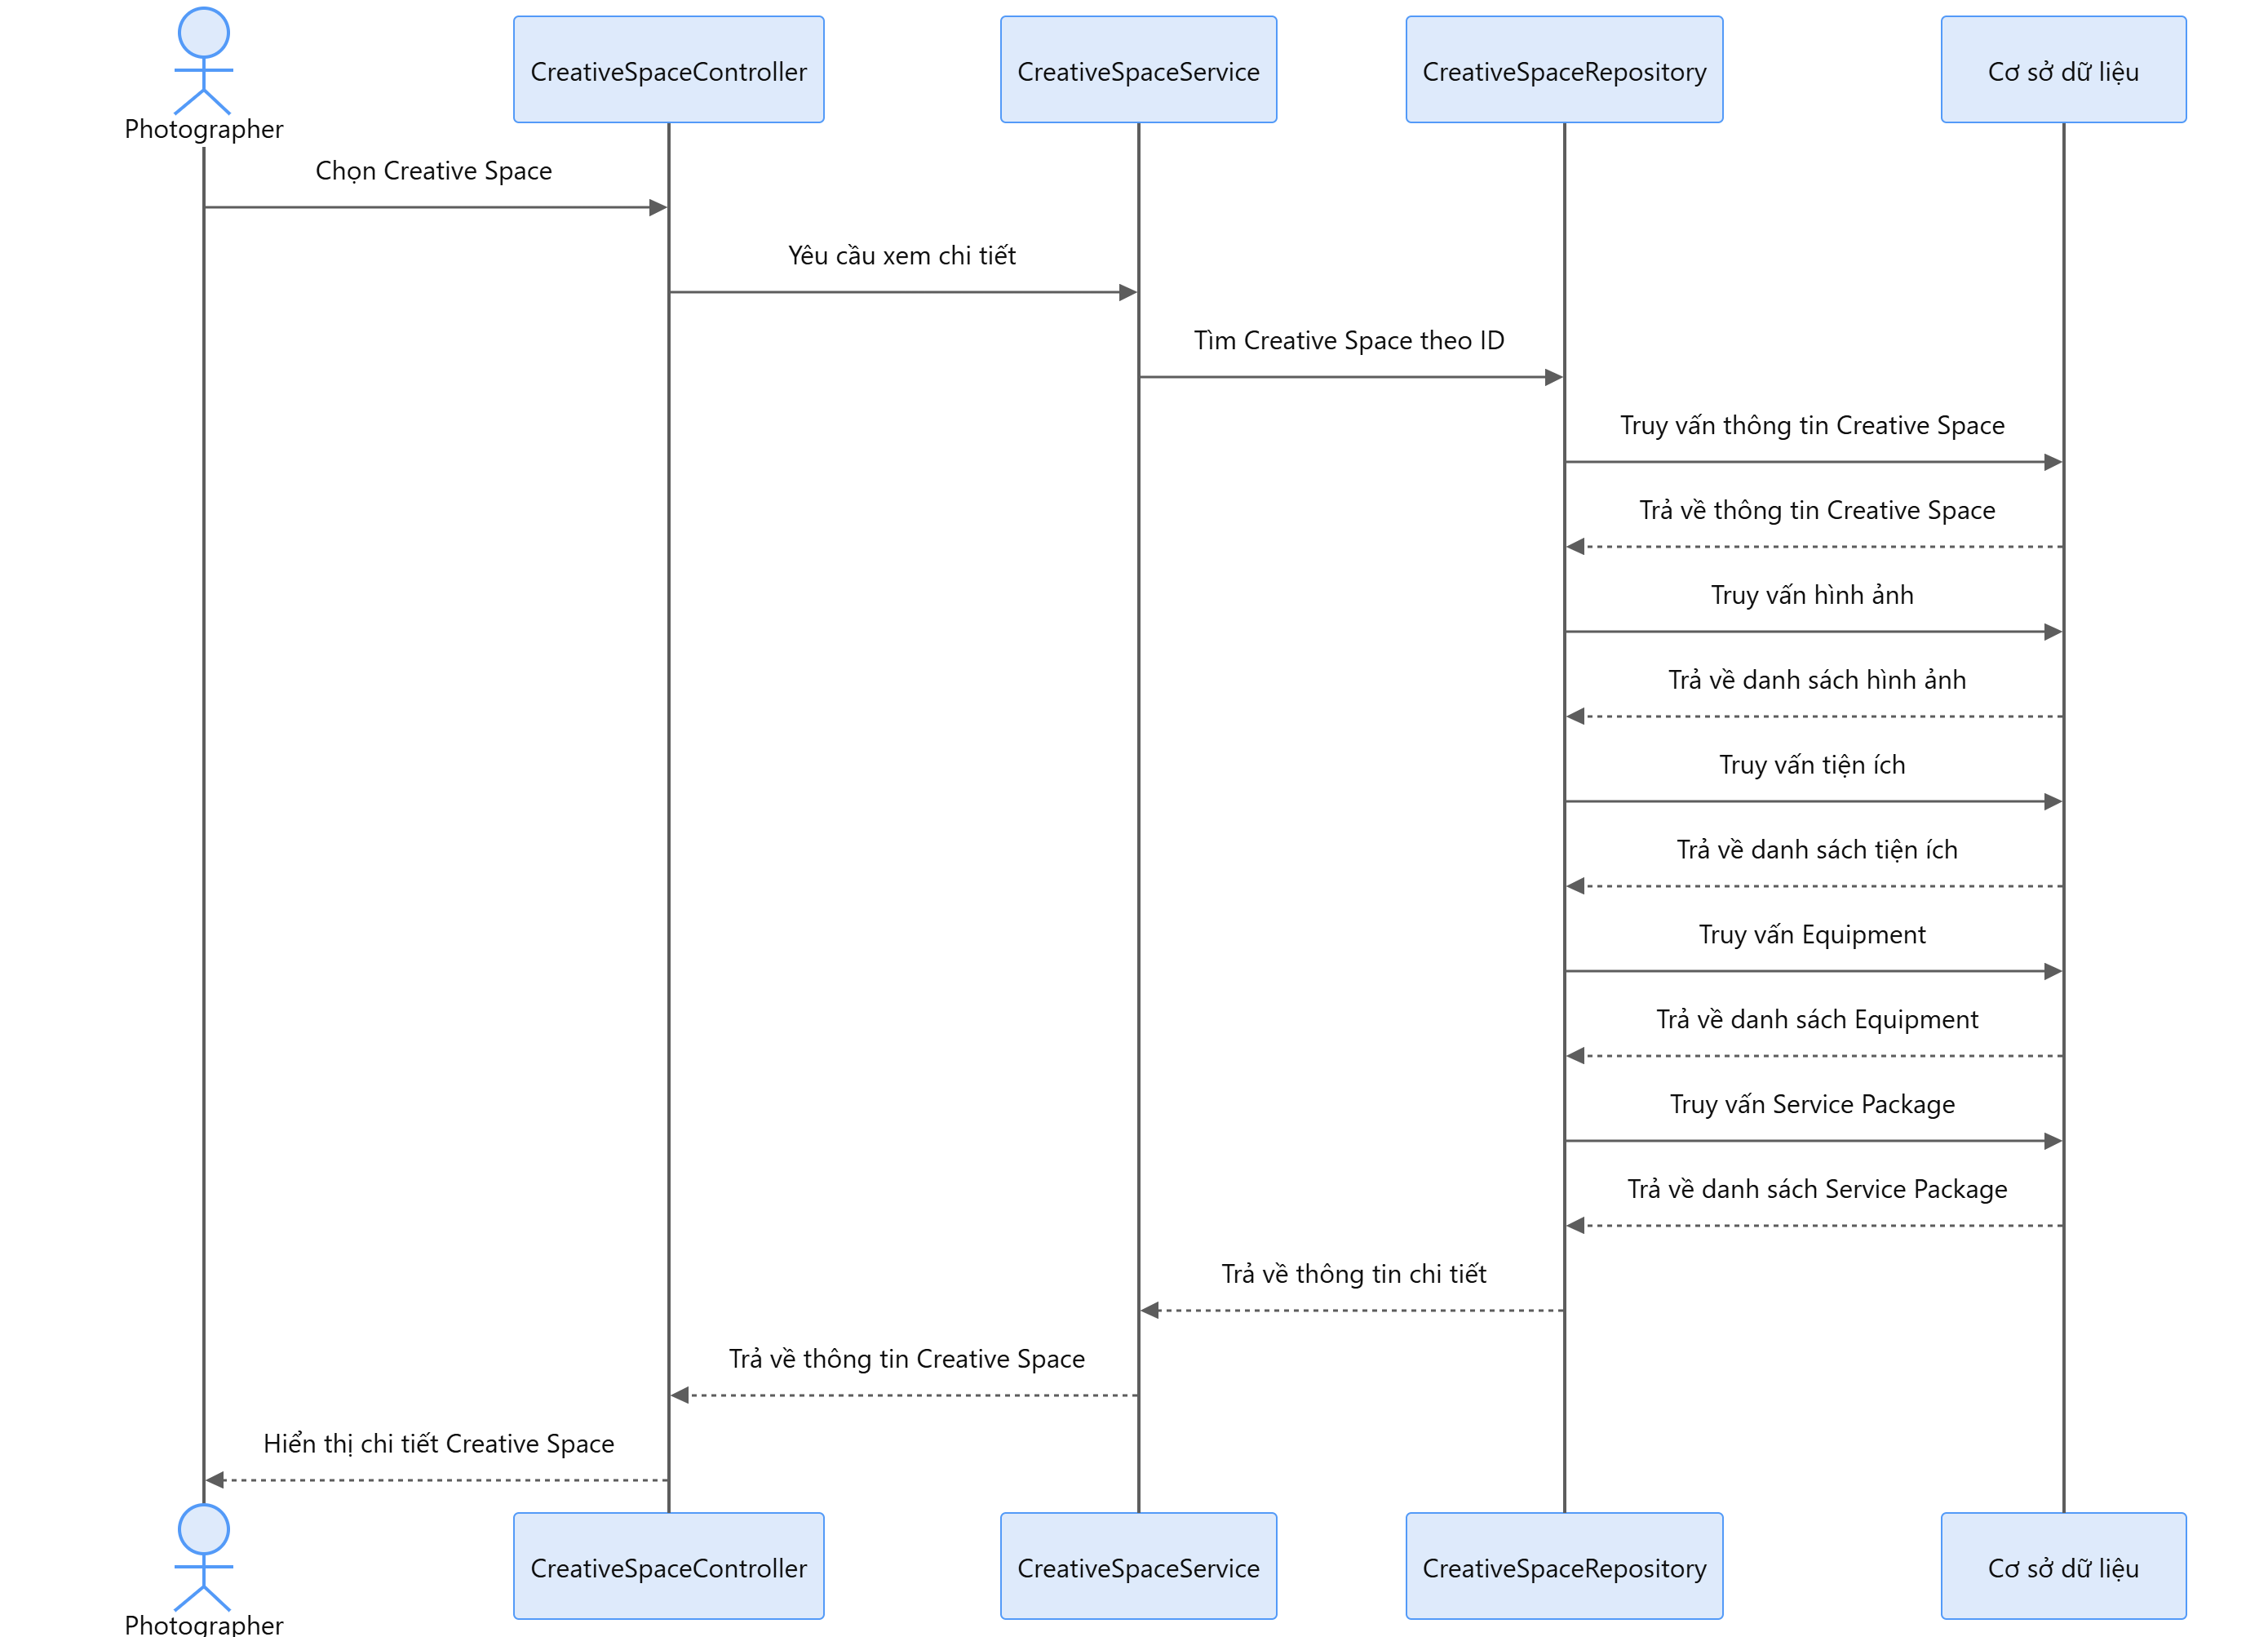
\includegraphics[width=1.1\textwidth]{images/25.png}
\end{figure}


% =========================================================
% 3.4 Reservation Management Module
% =========================================================

\subsection{Reservation Management Module}

\subsubsection{Đặt chỗ}

\paragraph{Class Diagram}

\begin{figure}[H]
	\centering
	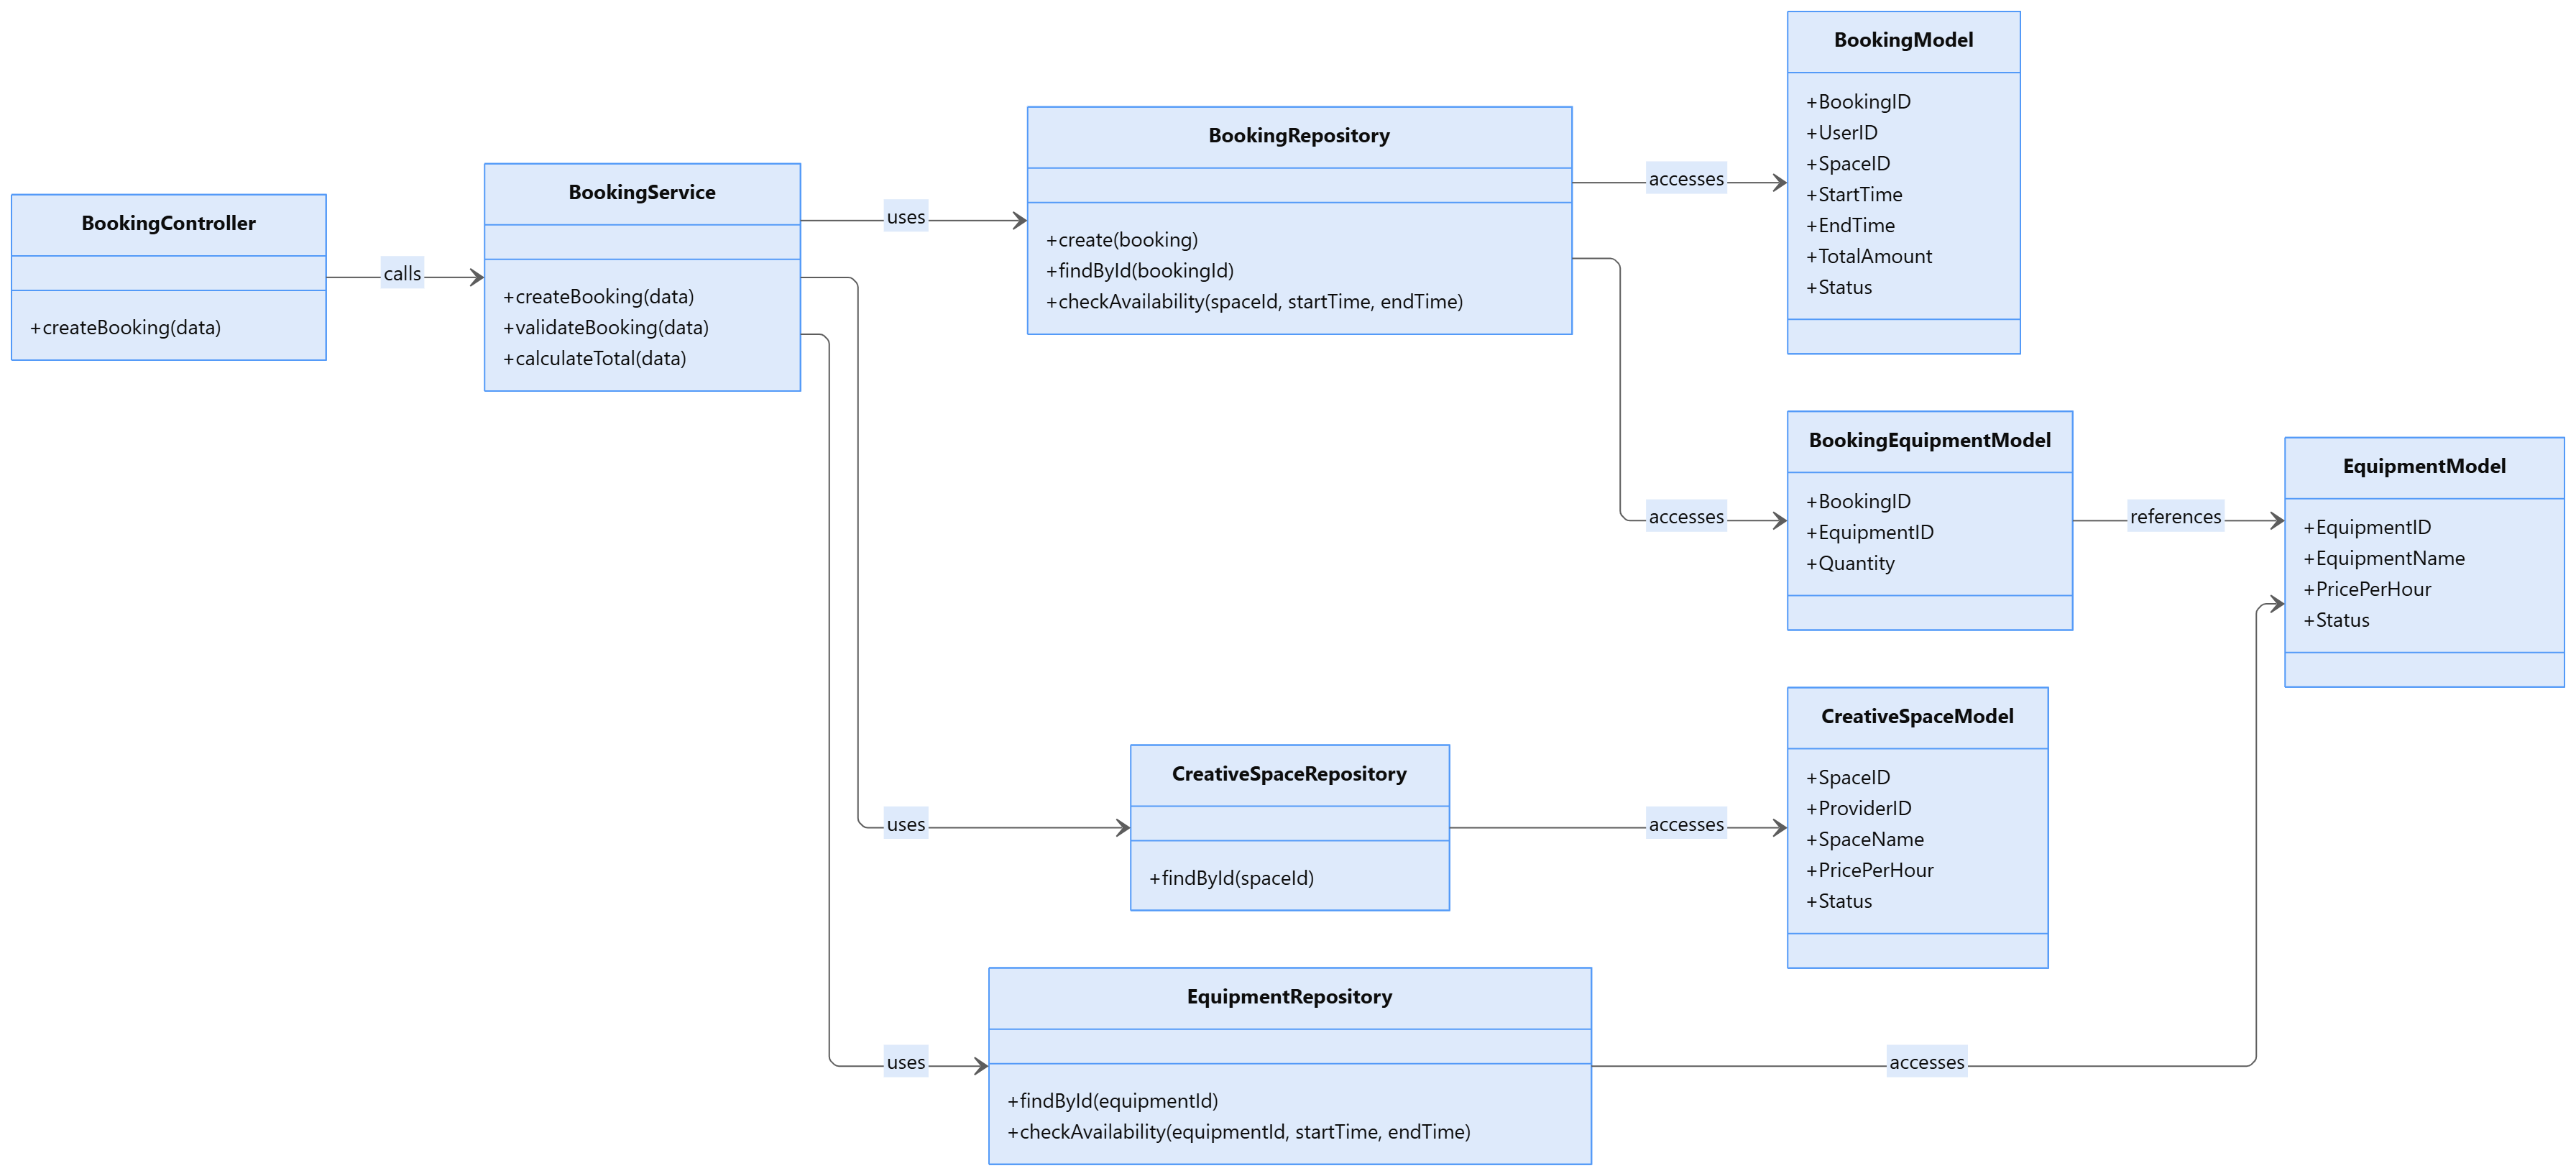
\includegraphics[width=1.1\textwidth]{images/26.png}
\end{figure}

\paragraph{Sequence Diagram}

\begin{figure}[H]
	\centering
	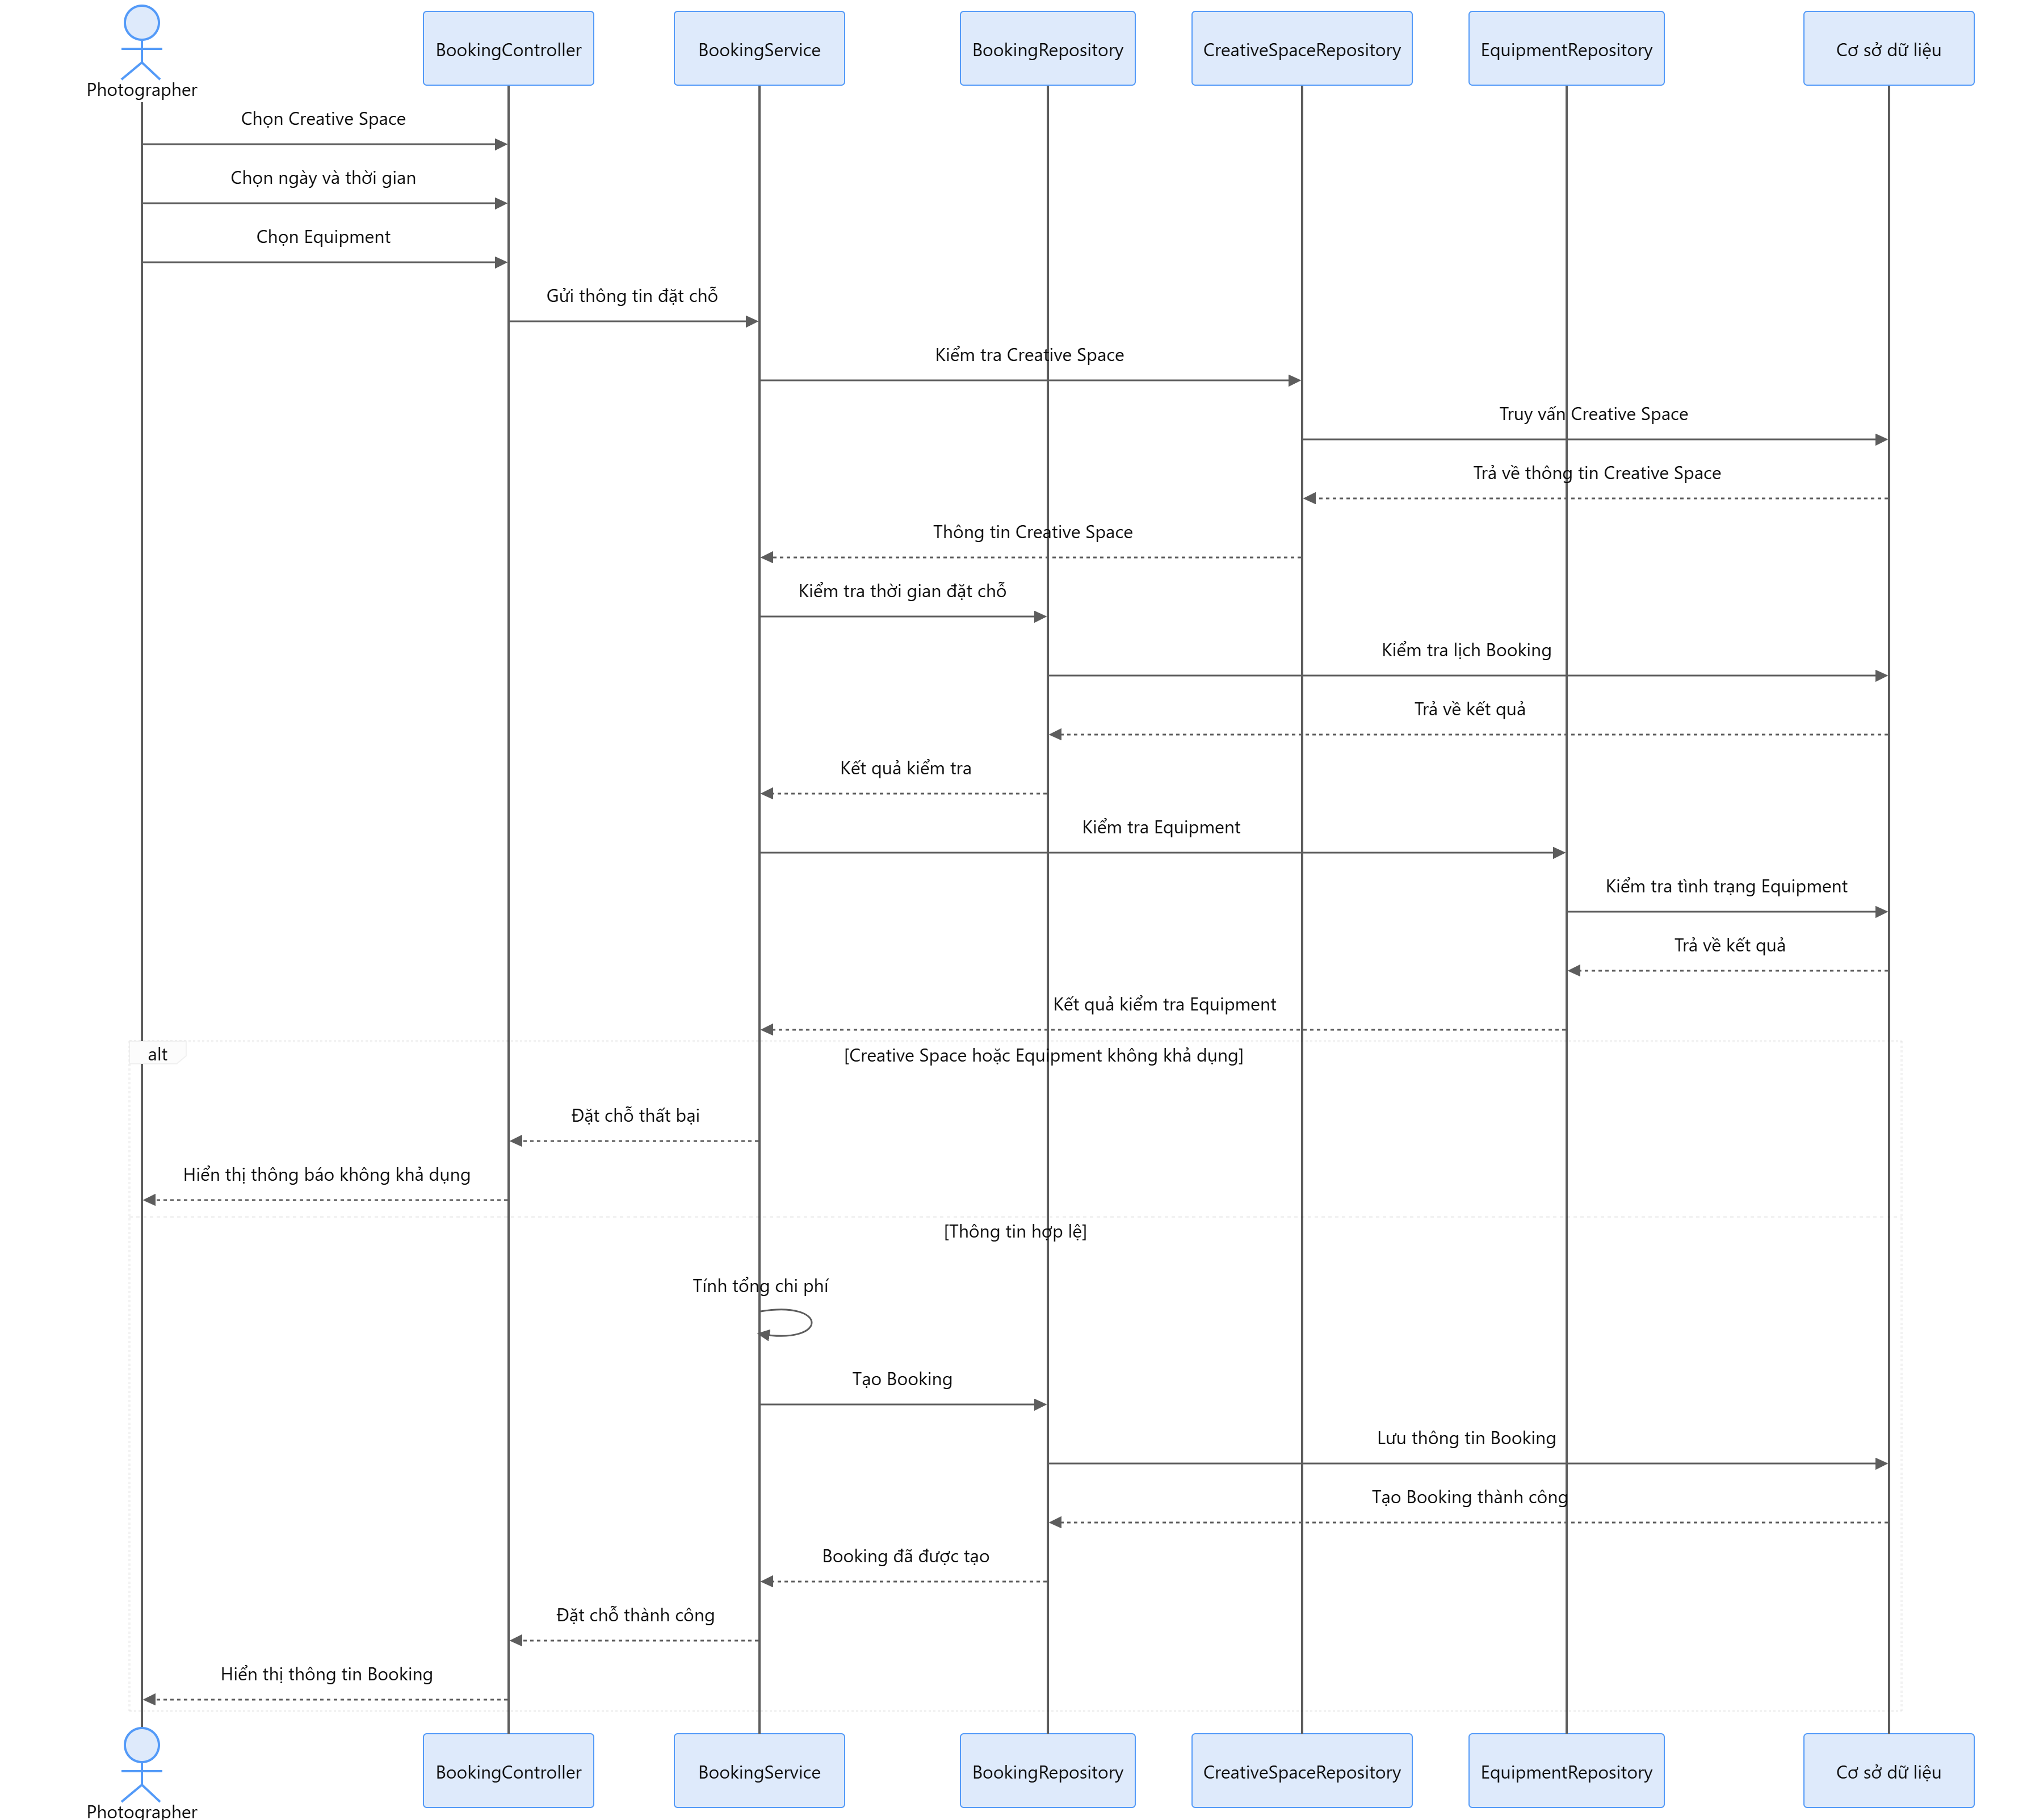
\includegraphics[width=1.1\textwidth]{images/27.png}
\end{figure}


\subsubsection{Hủy Booking}

\paragraph{Class Diagram}

\begin{figure}[H]
	\centering
	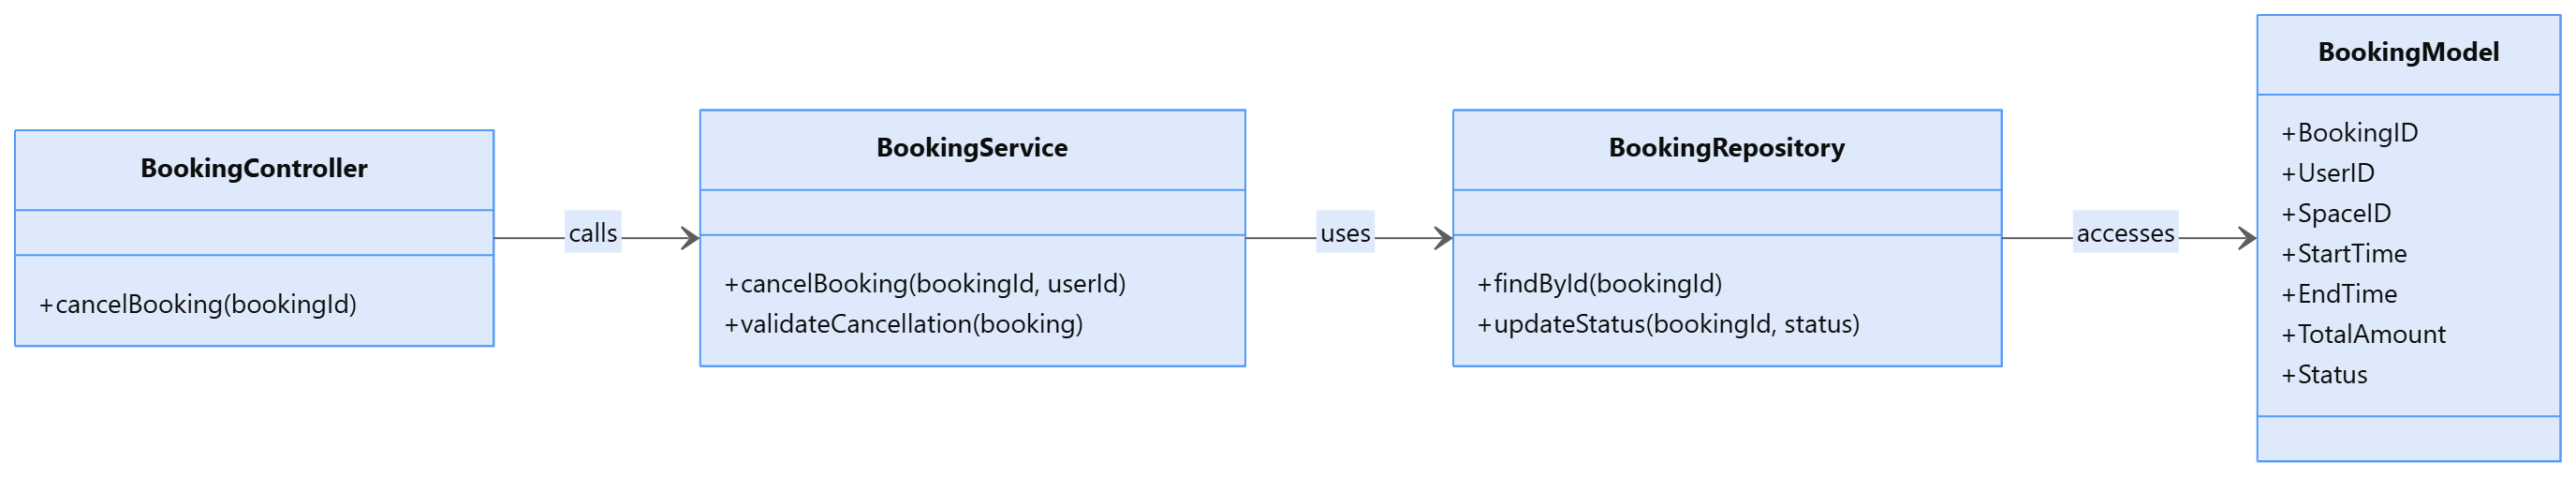
\includegraphics[width=1.1\textwidth]{images/28.png}
\end{figure}

\paragraph{Sequence Diagram}

\begin{figure}[H]
	\centering
	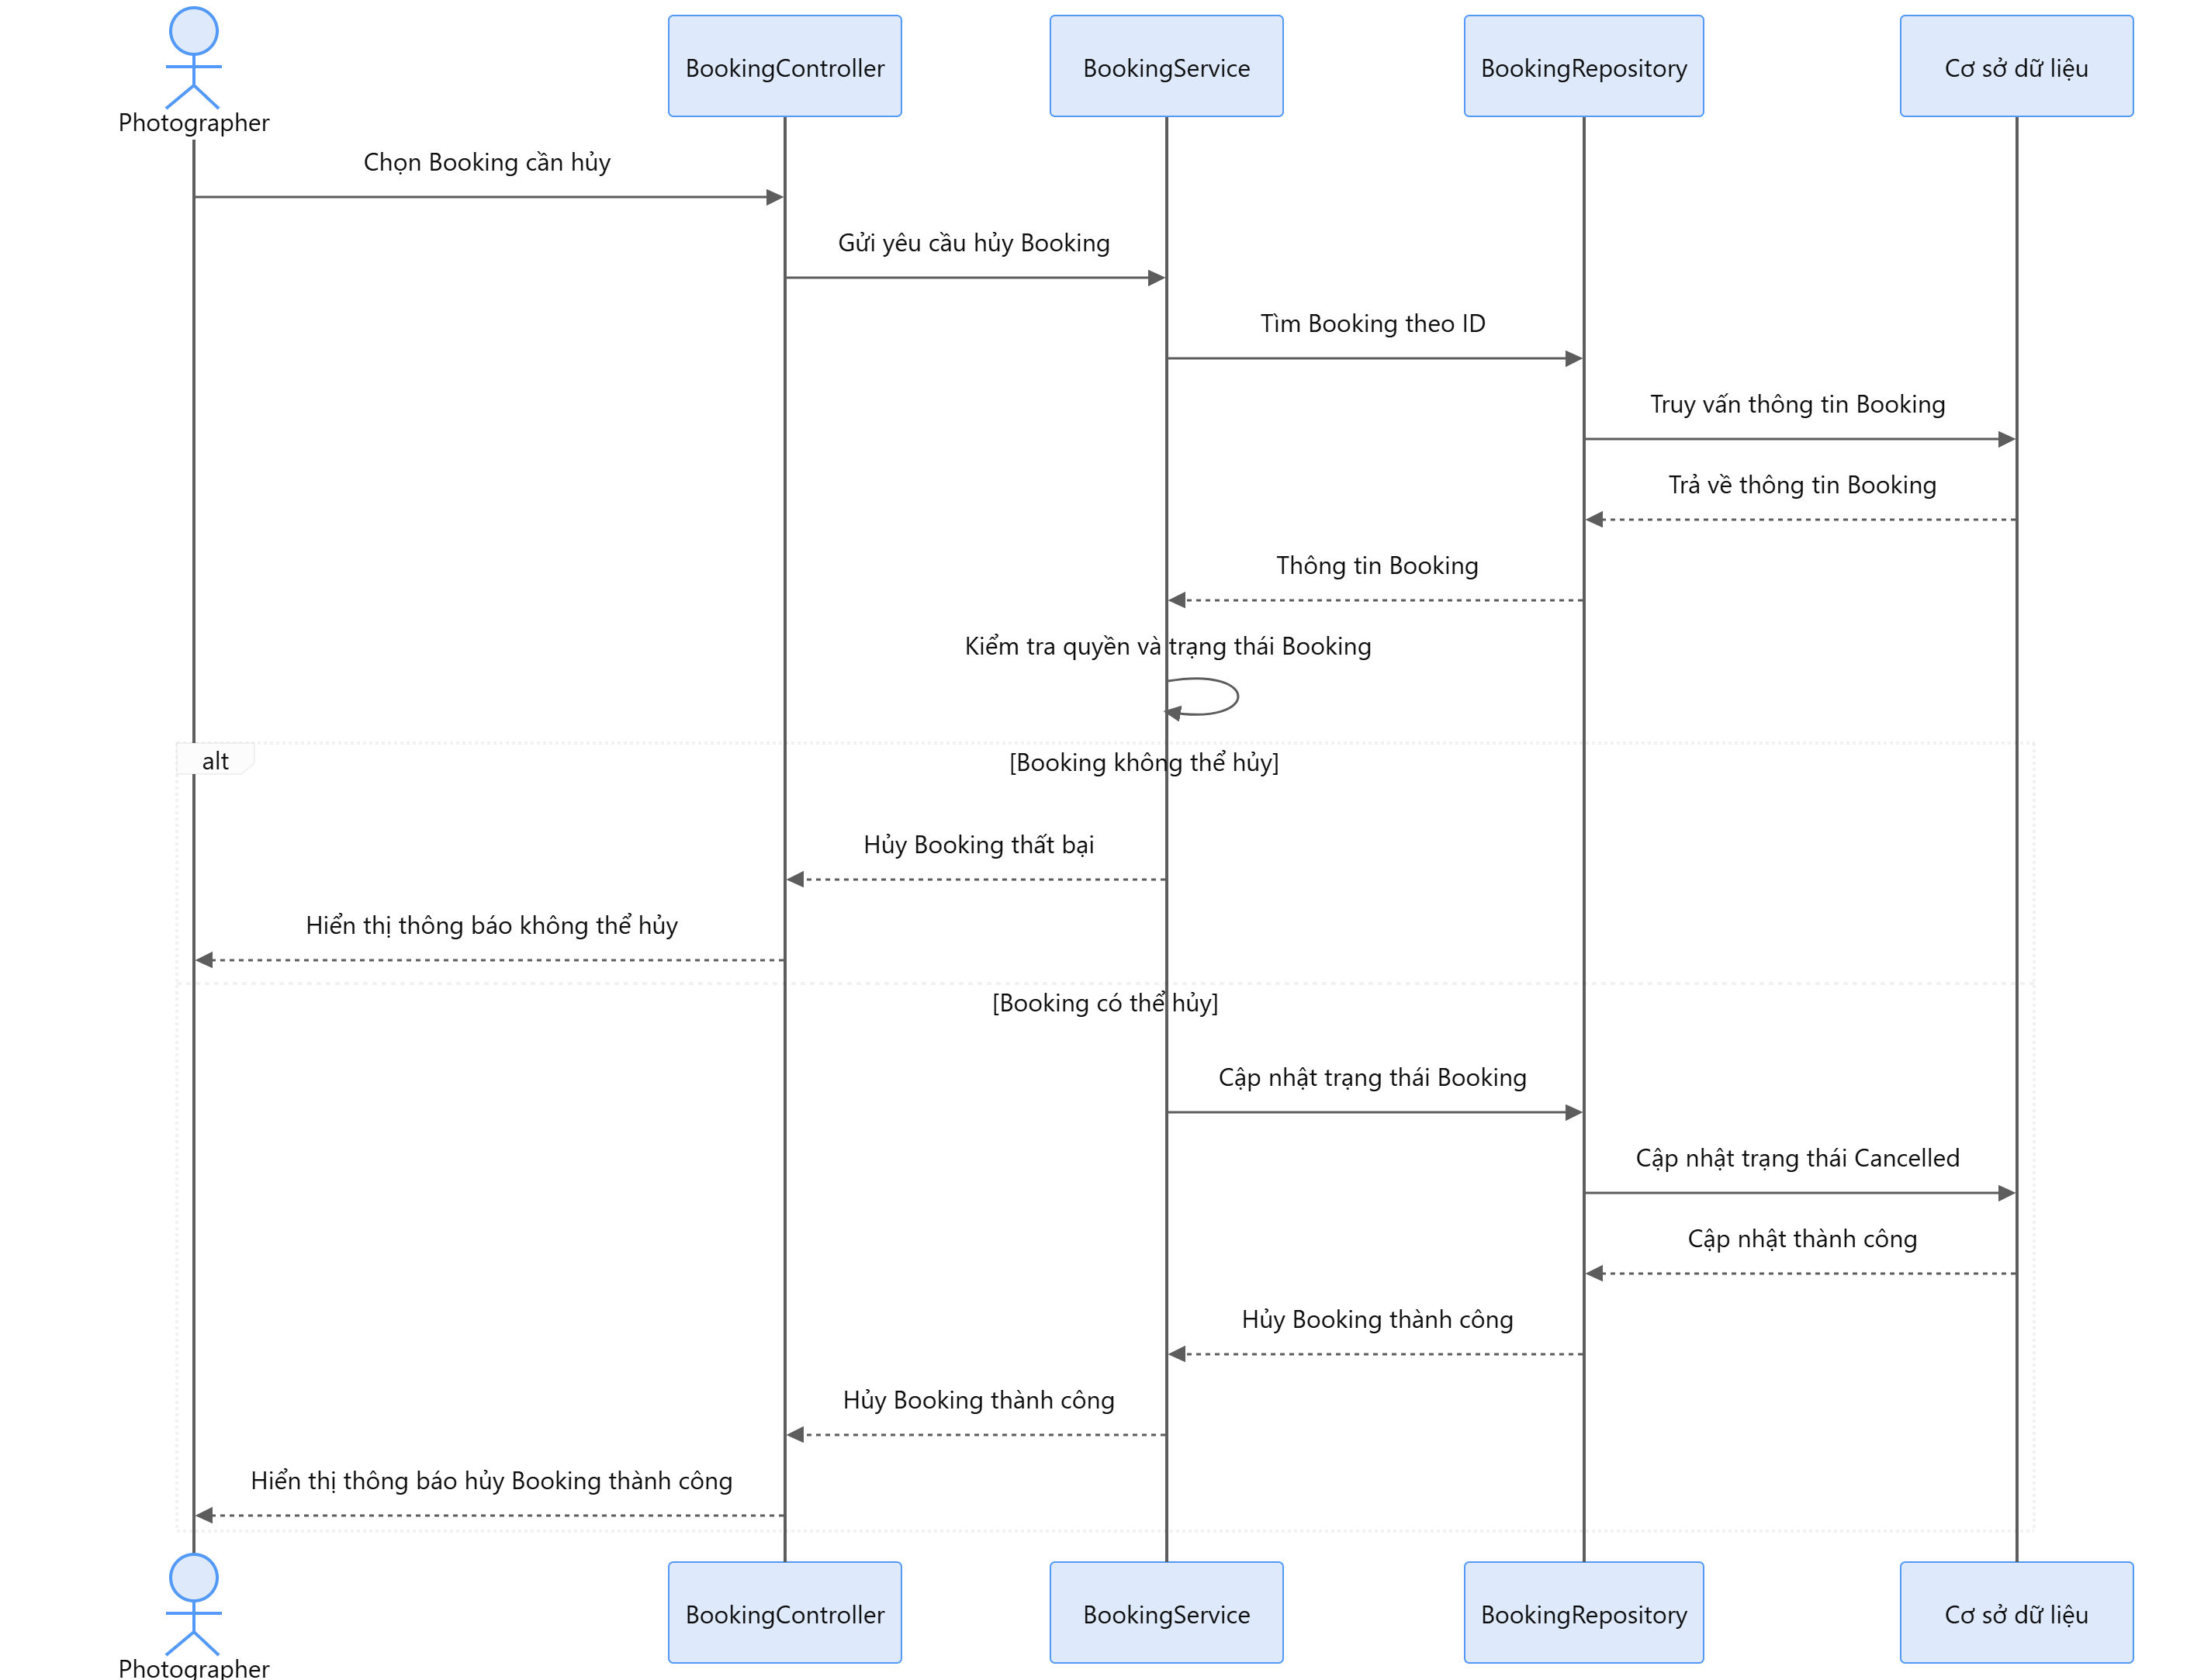
\includegraphics[width=1.1\textwidth]{images/29.png}
\end{figure}


% =========================================================
% 3.5 Payment and Booking Management Module
% =========================================================

\subsection{Payment and Booking Management Module}

\subsubsection{Thanh toán}

\paragraph{Class Diagram}

\begin{figure}[H]
	\centering
	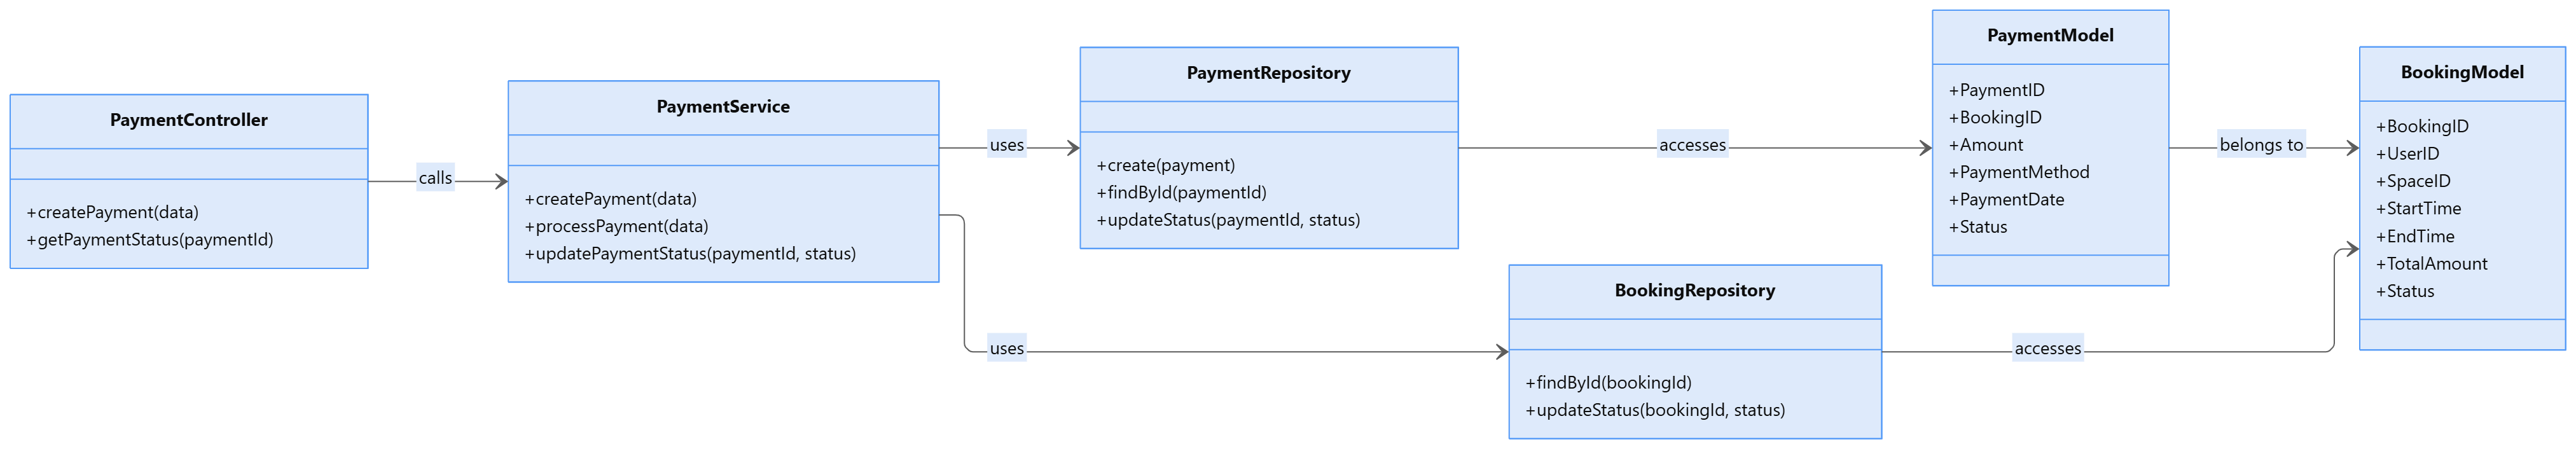
\includegraphics[width=1.1\textwidth]{images/30.png}
\end{figure}

\paragraph{Sequence Diagram}

\begin{figure}[H]
	\centering
	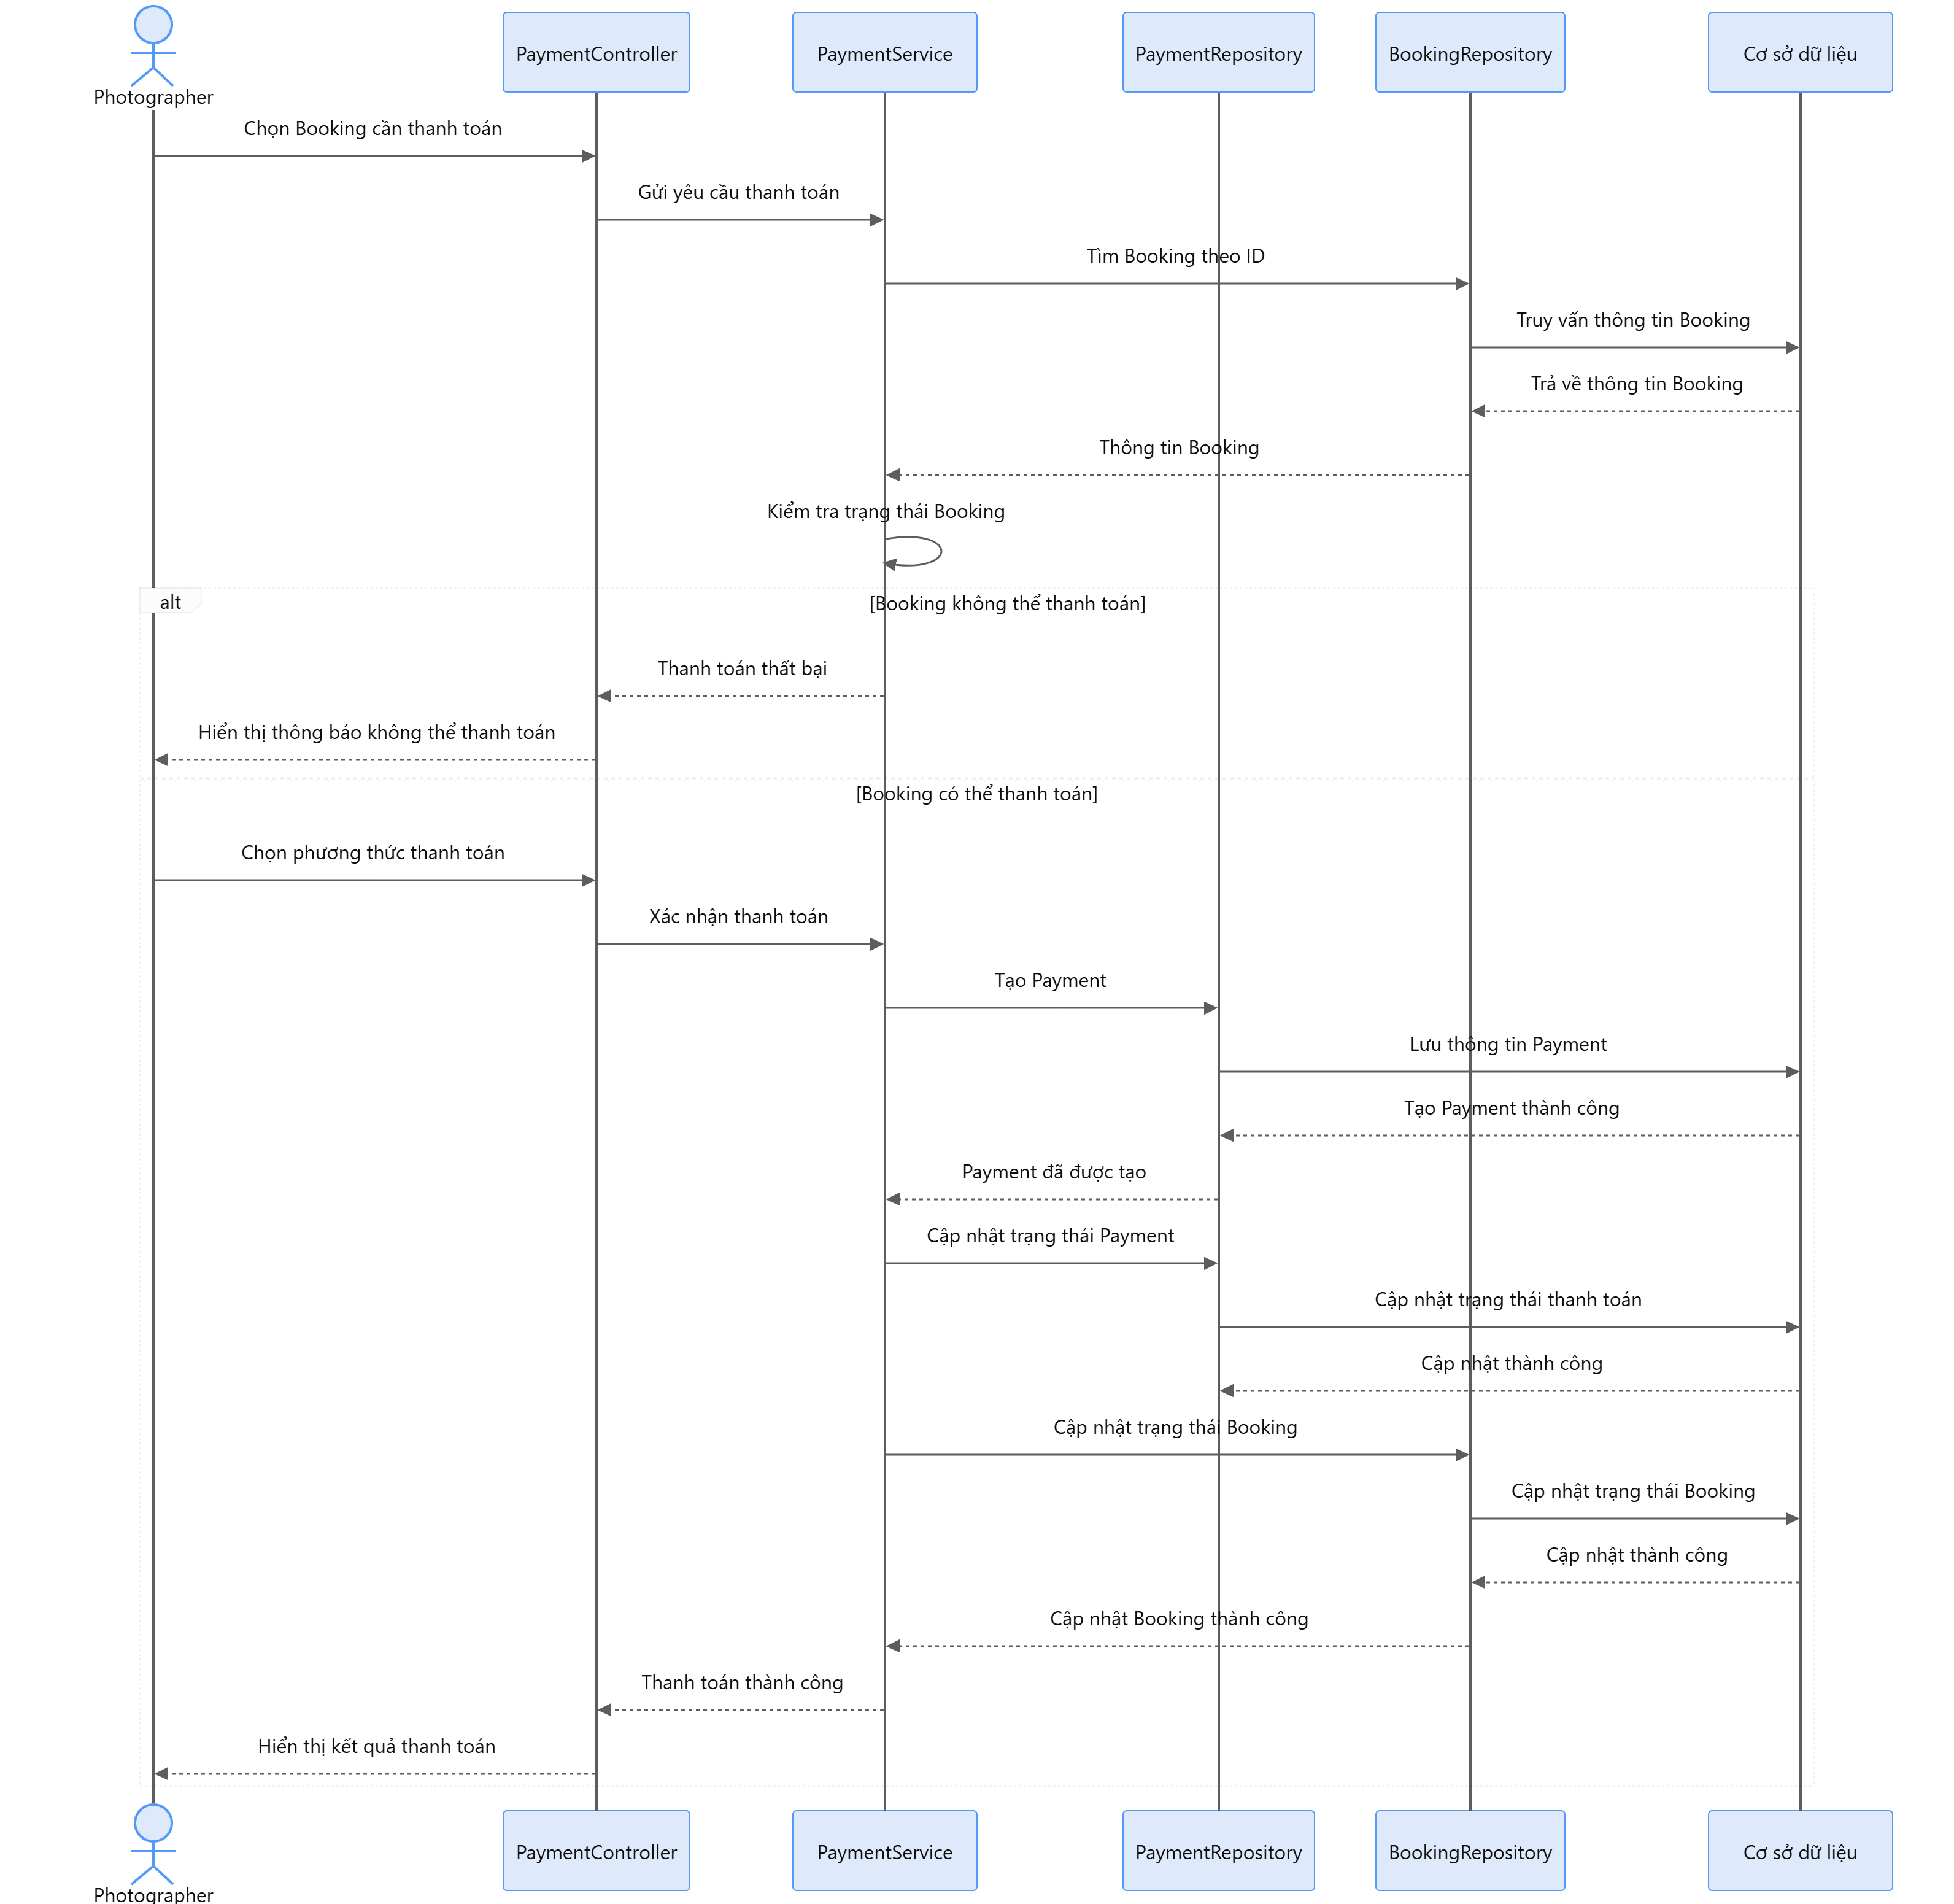
\includegraphics[width=1.1\textwidth]{images/31.png}
\end{figure}


% =========================================================
% 3.6 Workshop Management Module
% =========================================================

\subsection{Workshop Management Module}

\subsubsection{Đăng ký Workshop}

\paragraph{Class Diagram}

\begin{figure}[H]
	\centering
	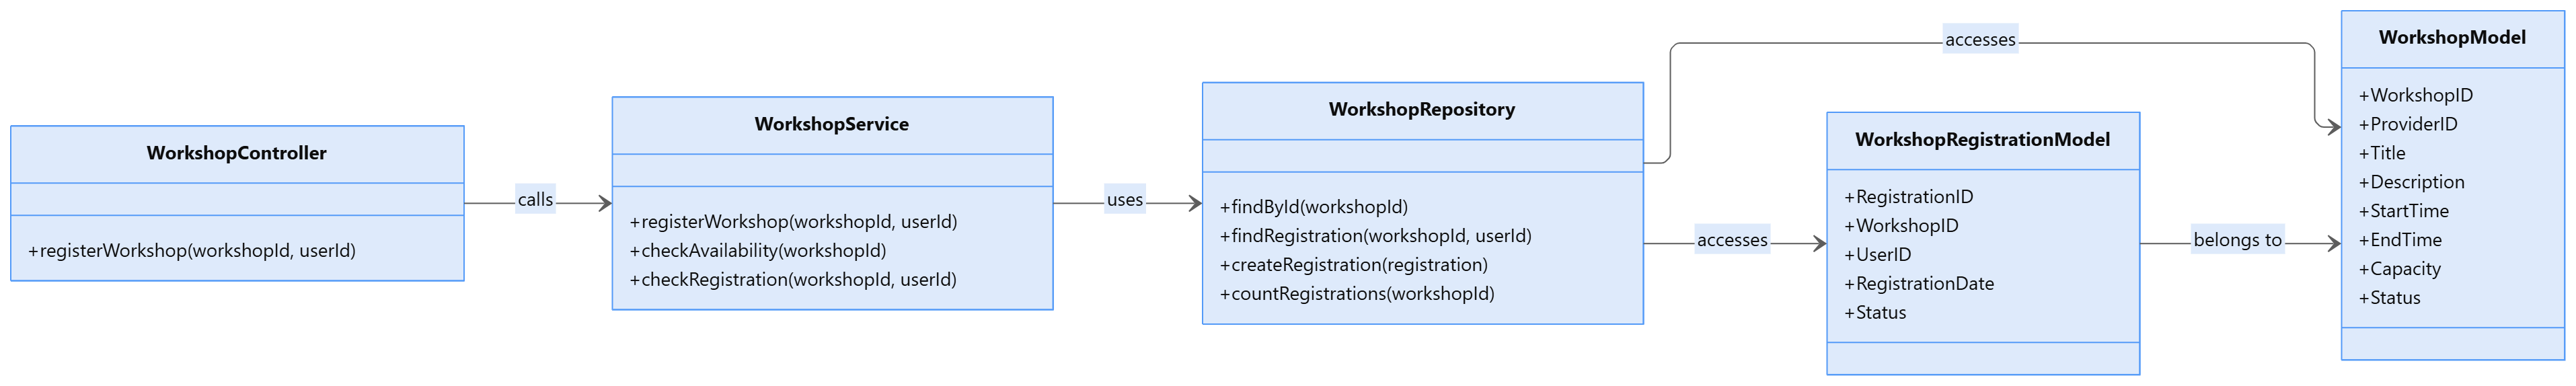
\includegraphics[width=1.1\textwidth]{images/32.png}
\end{figure}

\paragraph{Sequence Diagram}

\begin{figure}[H]
	\centering
	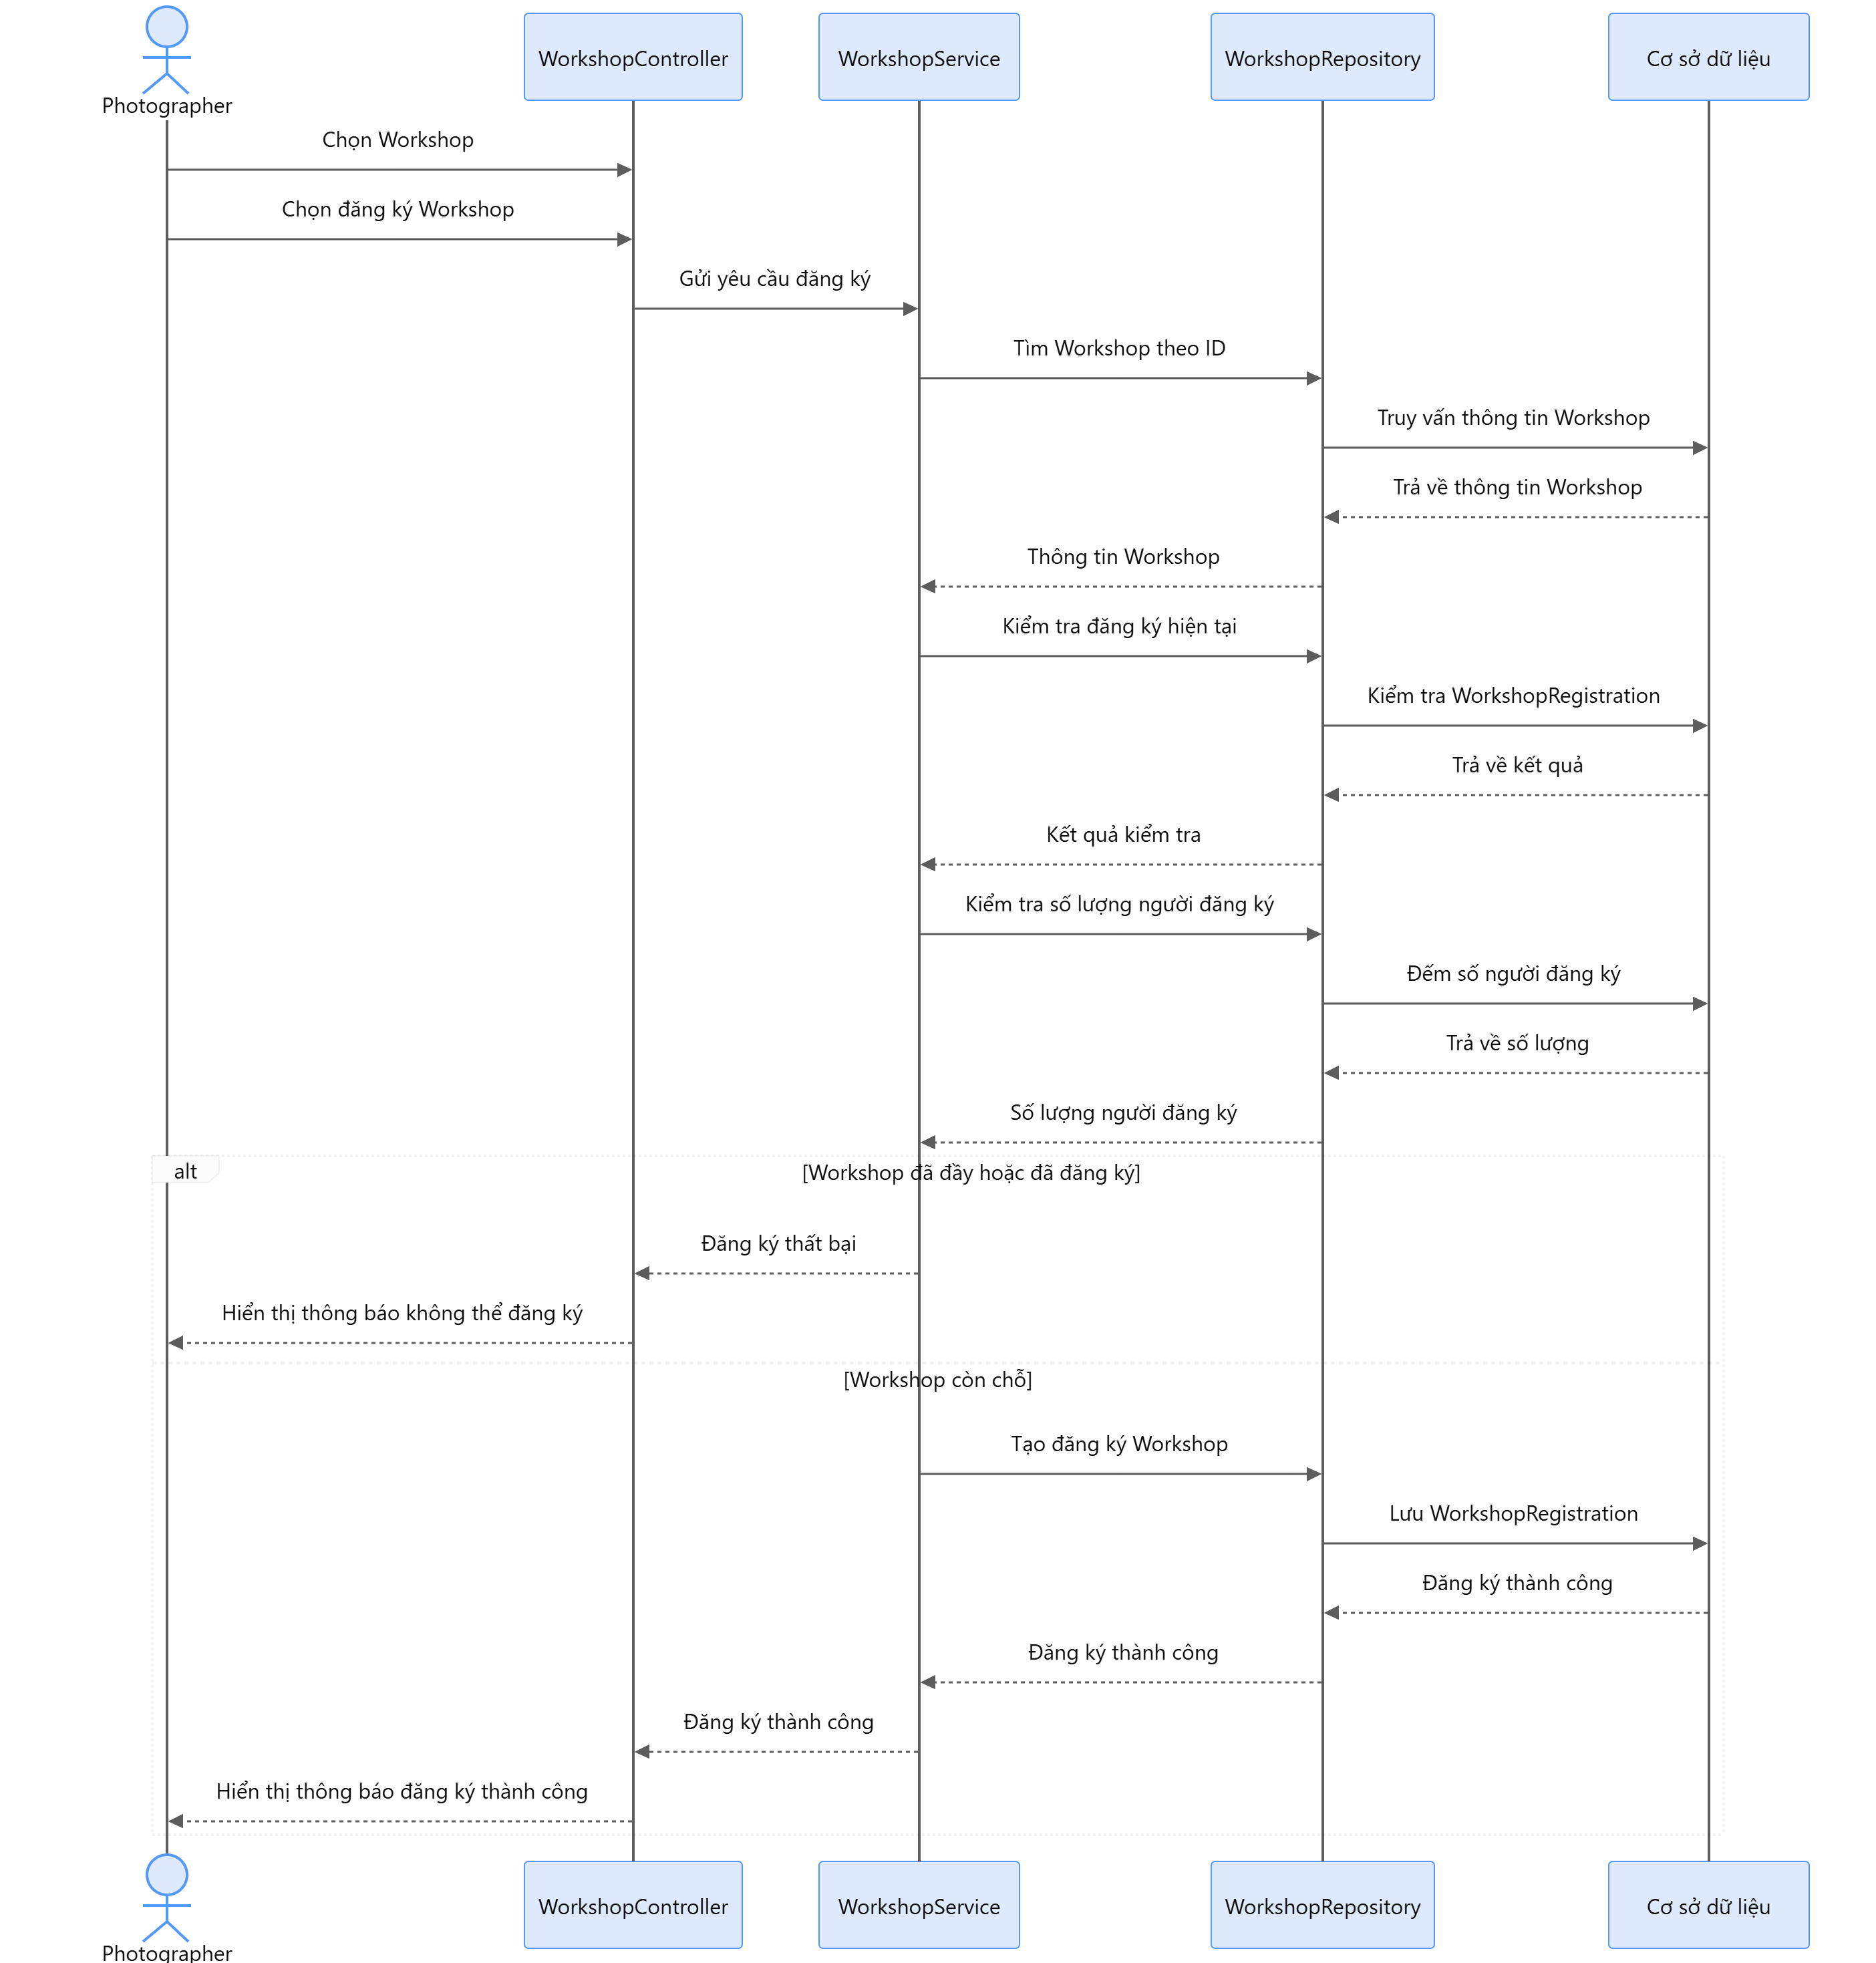
\includegraphics[width=1.1\textwidth]{images/33.png}
\end{figure}


% =========================================================
% 3.7 Service Provider Management Module
% =========================================================

\subsection{Service Provider Management Module}

\subsubsection{Quản lý hồ sơ Provider}

\paragraph{Class Diagram}

\begin{figure}[H]
	\centering
	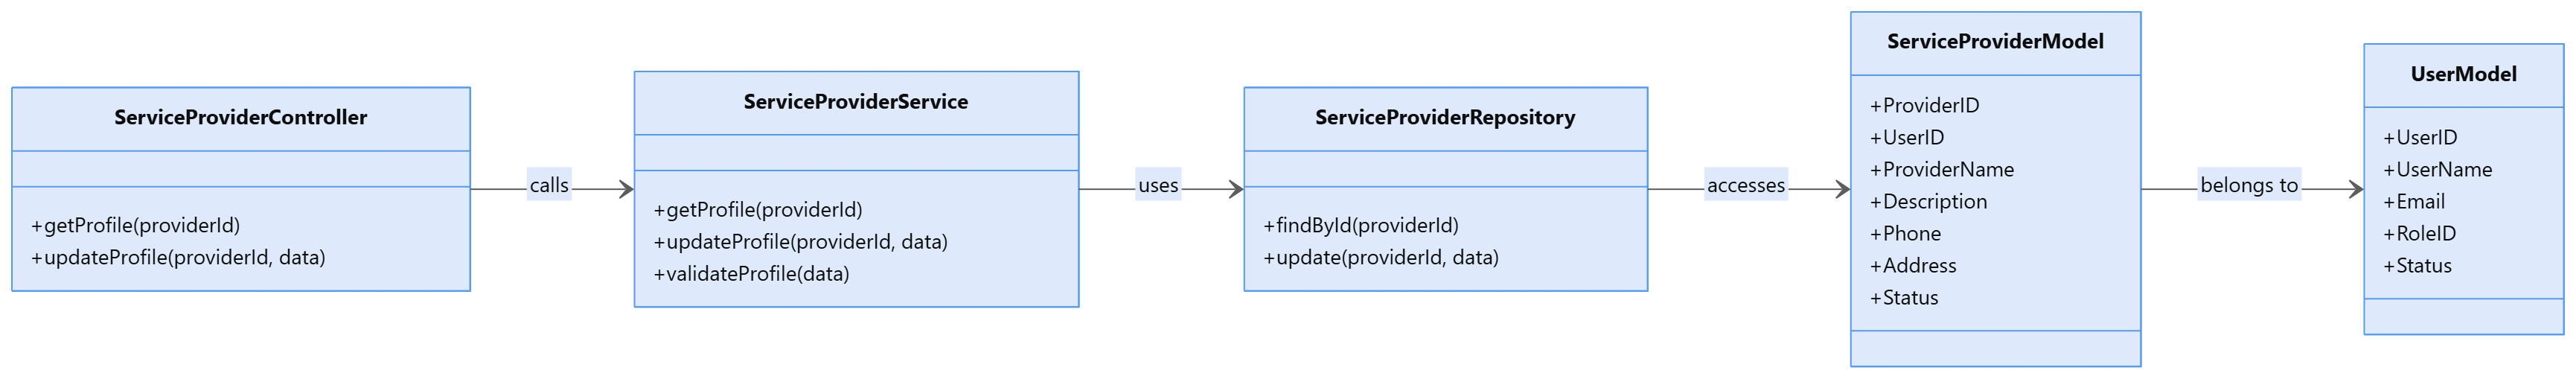
\includegraphics[width=1.1\textwidth]{images/34.png}
\end{figure}

\paragraph{Sequence Diagram}

\begin{figure}[H]
	\centering
	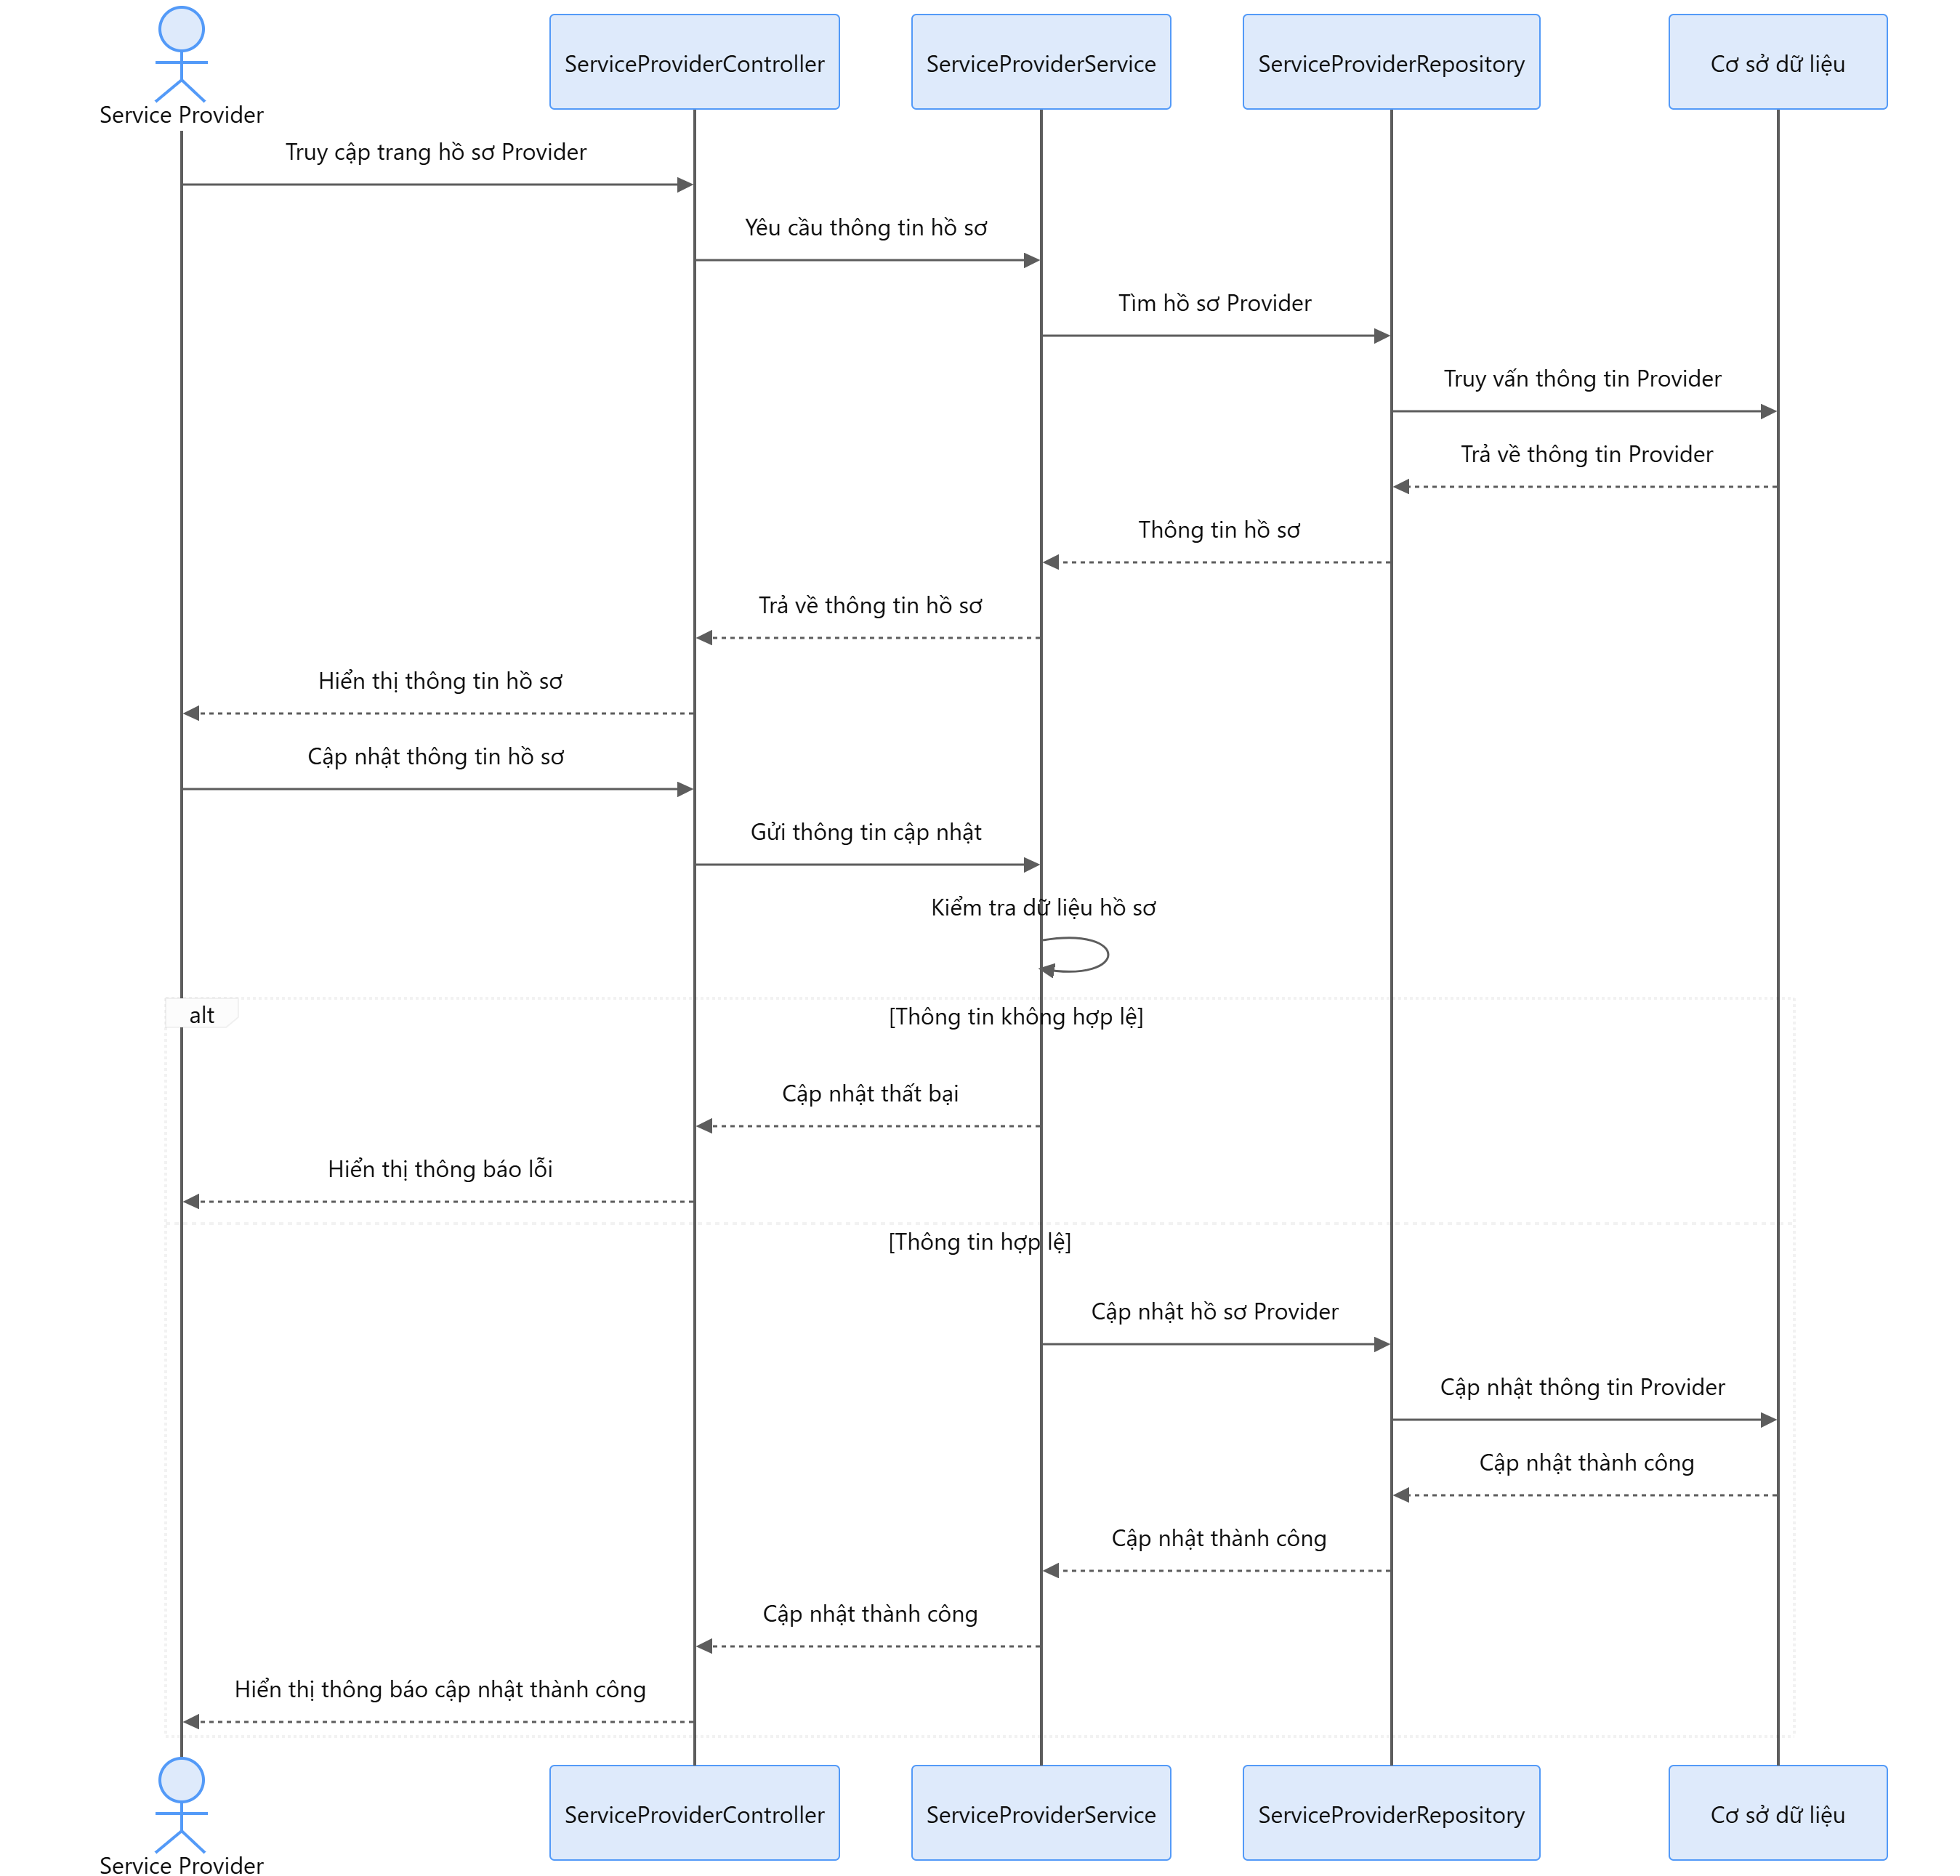
\includegraphics[width=1.1\textwidth]{images/35.png}
\end{figure}


\subsubsection{Quản lý Creative Space}

\paragraph{Class Diagram}

\begin{figure}[H]
	\centering
	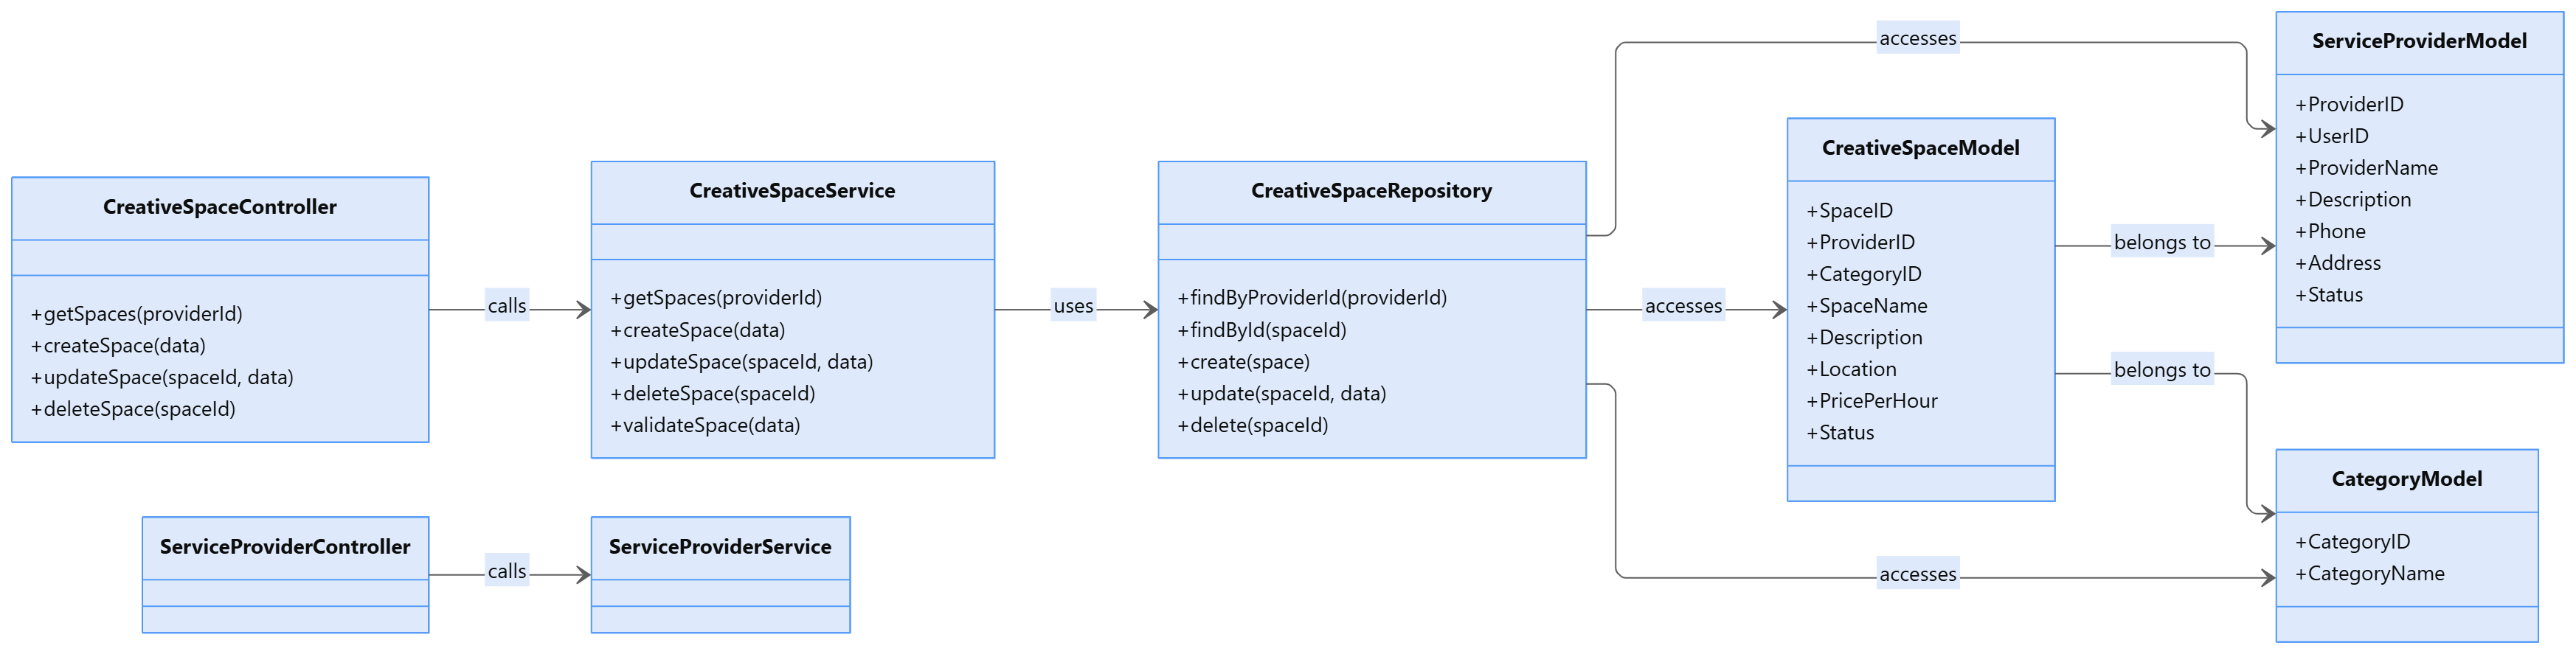
\includegraphics[width=1.1\textwidth]{images/36.png}
\end{figure}

\paragraph{Sequence Diagram}

\begin{figure}[H]
	\centering
	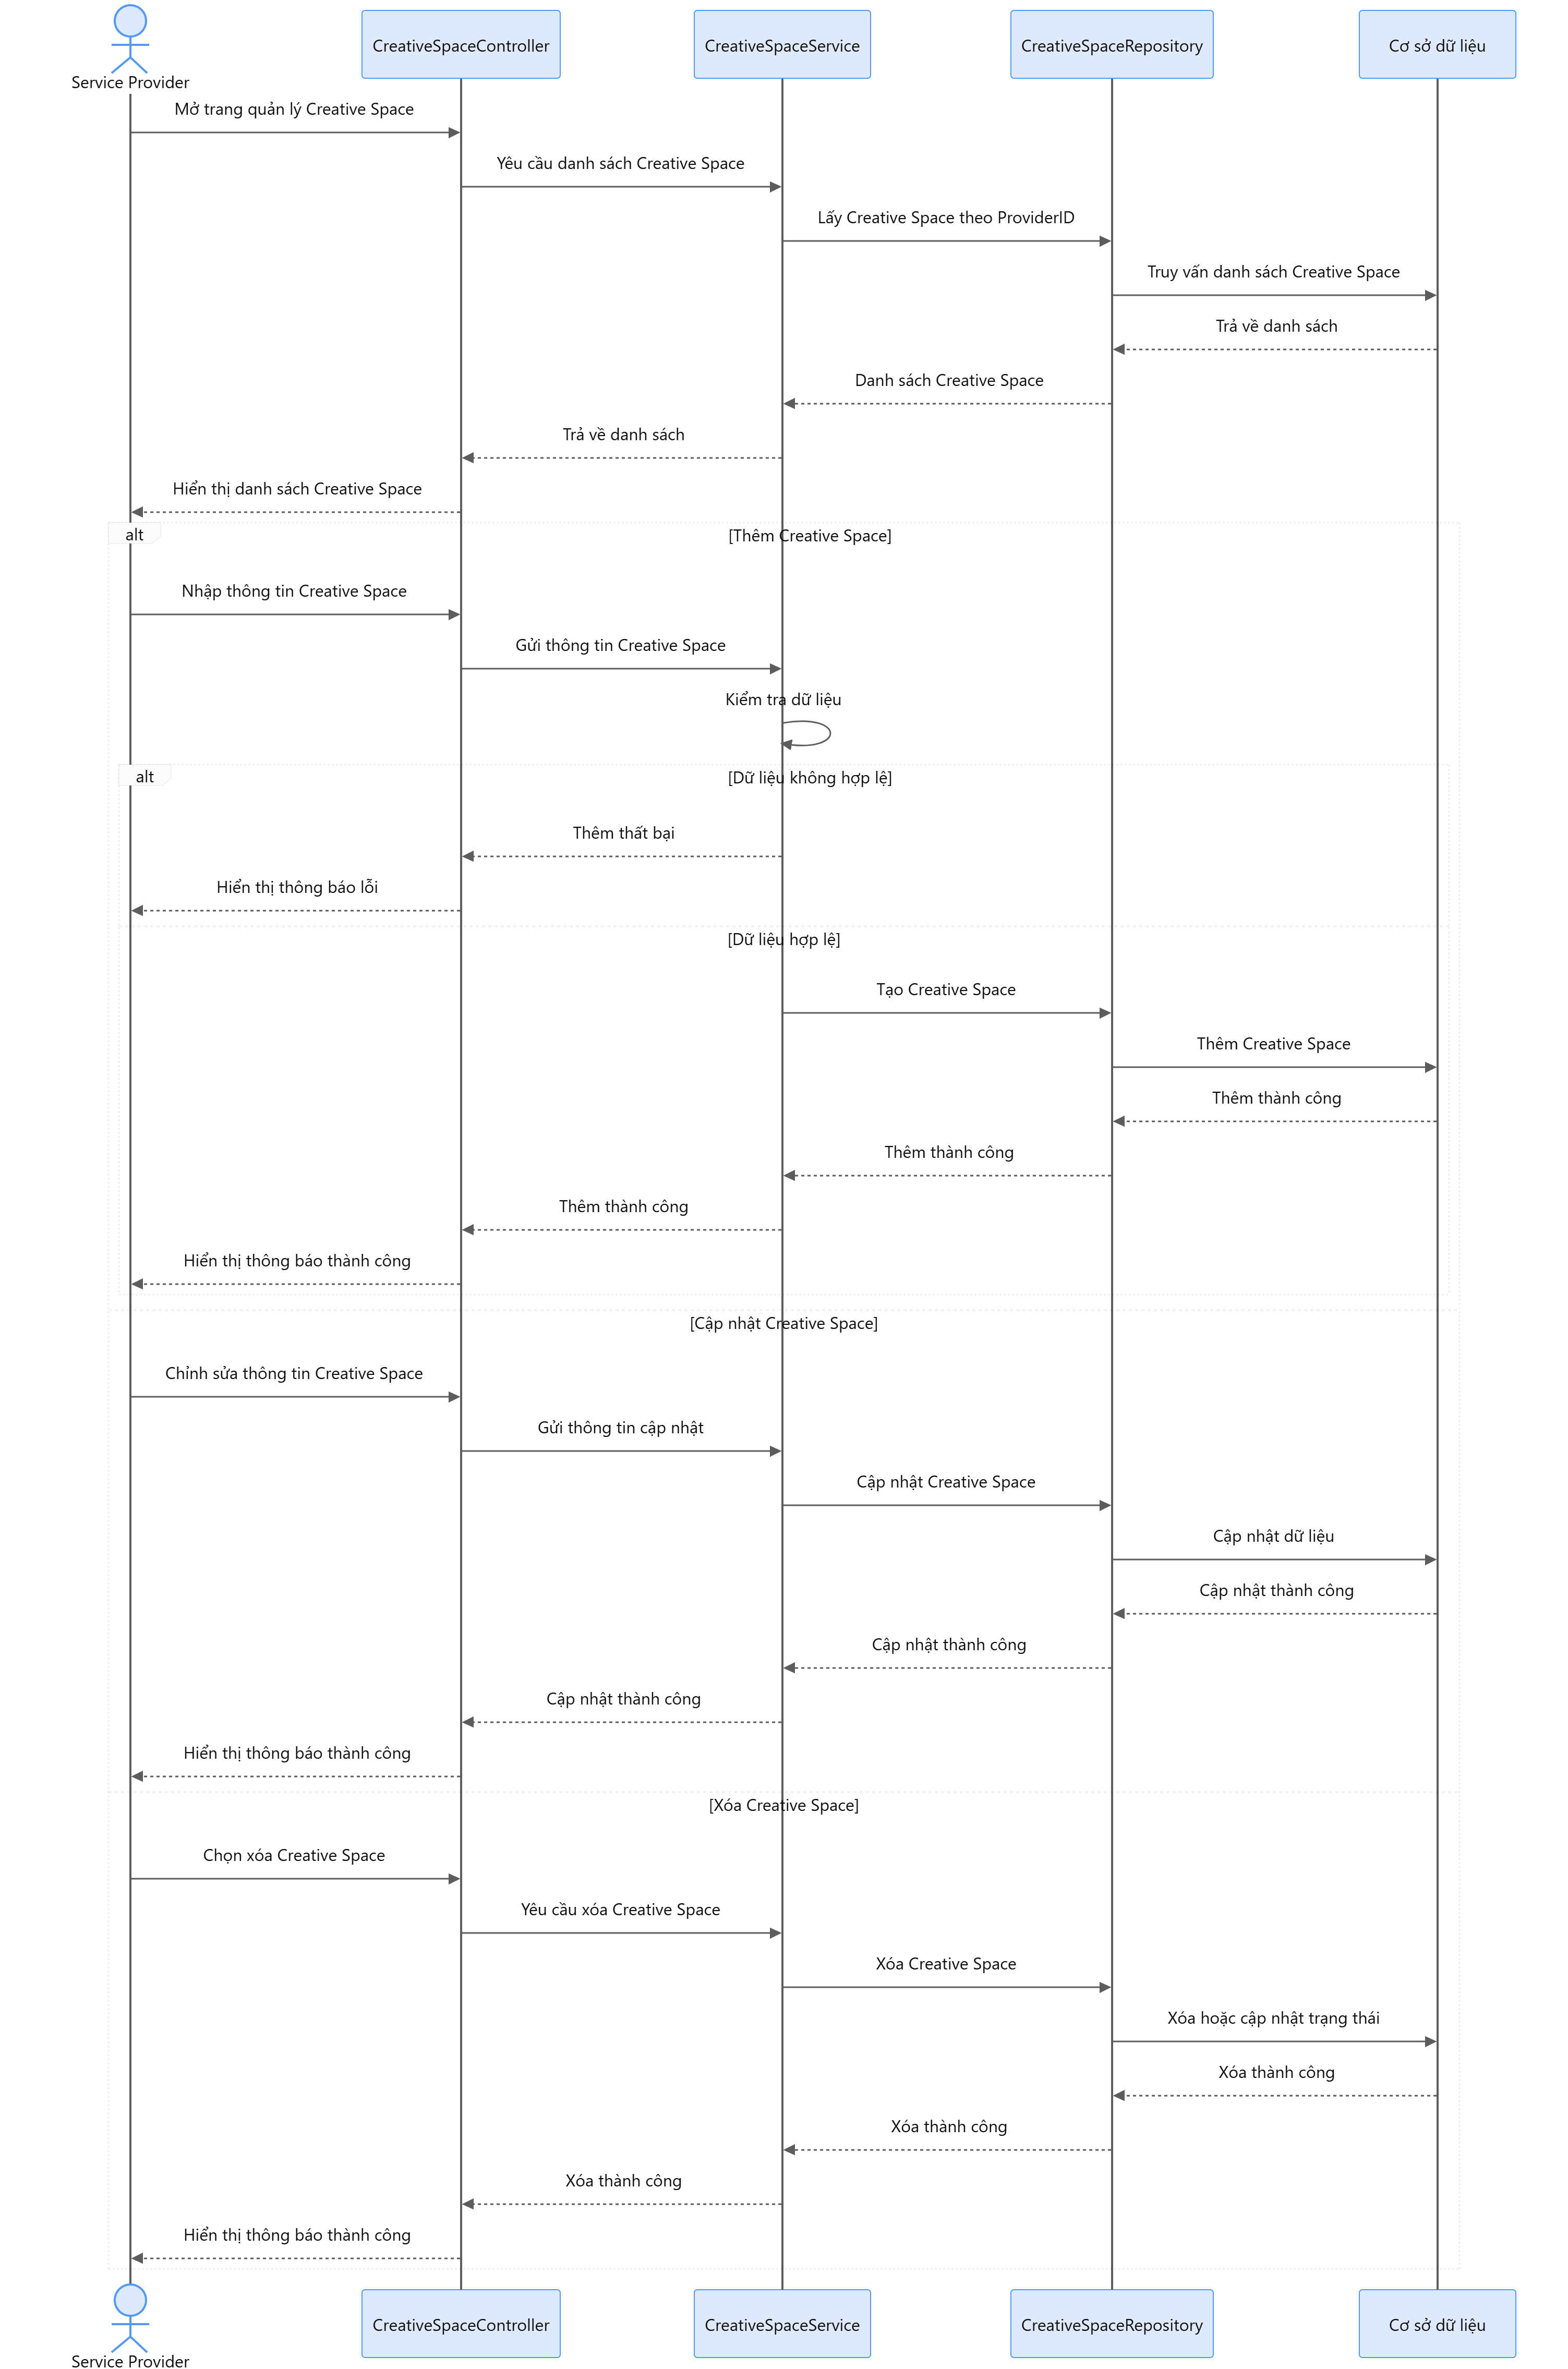
\includegraphics[width=1.1\textwidth]{images/37.png}
\end{figure}


\subsubsection{Quản lý Equipment}

\paragraph{Class Diagram}

\begin{figure}[H]
	\centering
	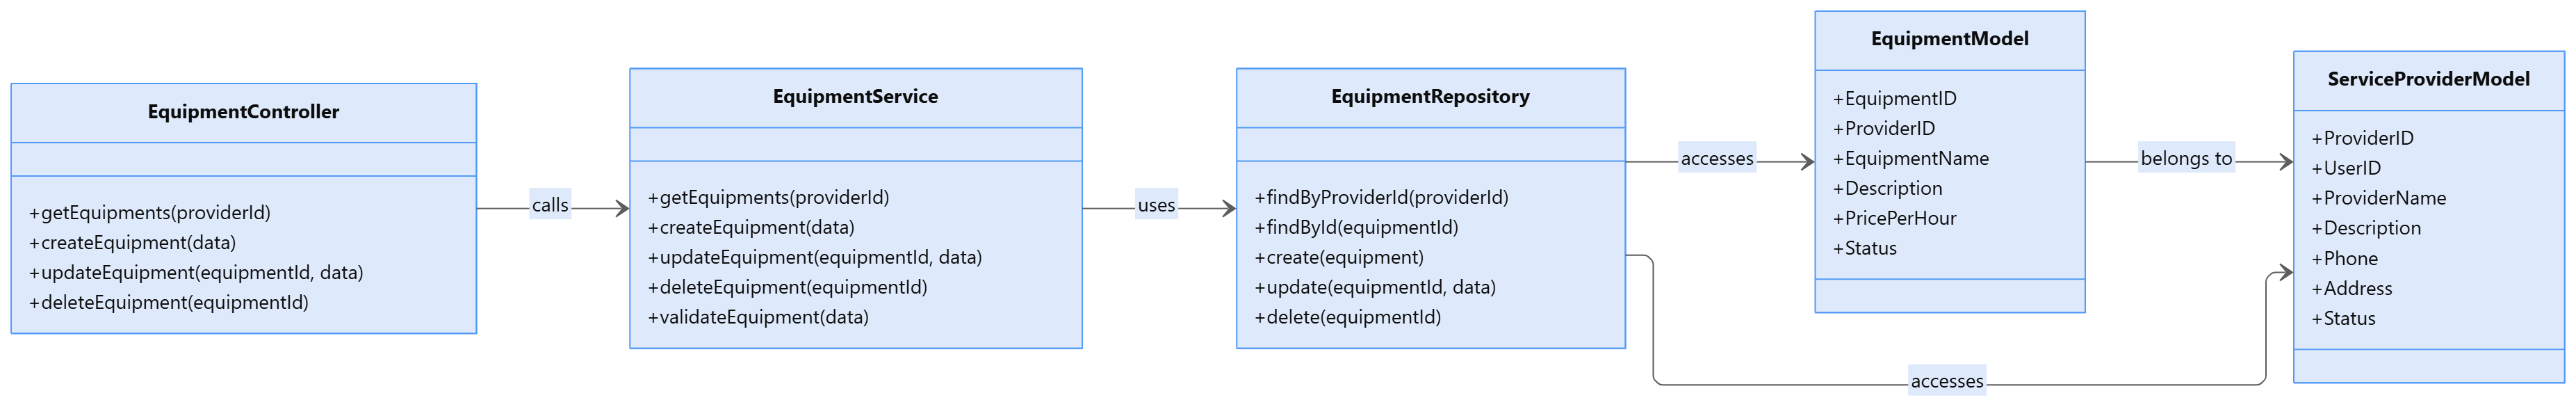
\includegraphics[width=1.1\textwidth]{images/38.png}
\end{figure}

\paragraph{Sequence Diagram}

\begin{figure}[H]
	\centering
	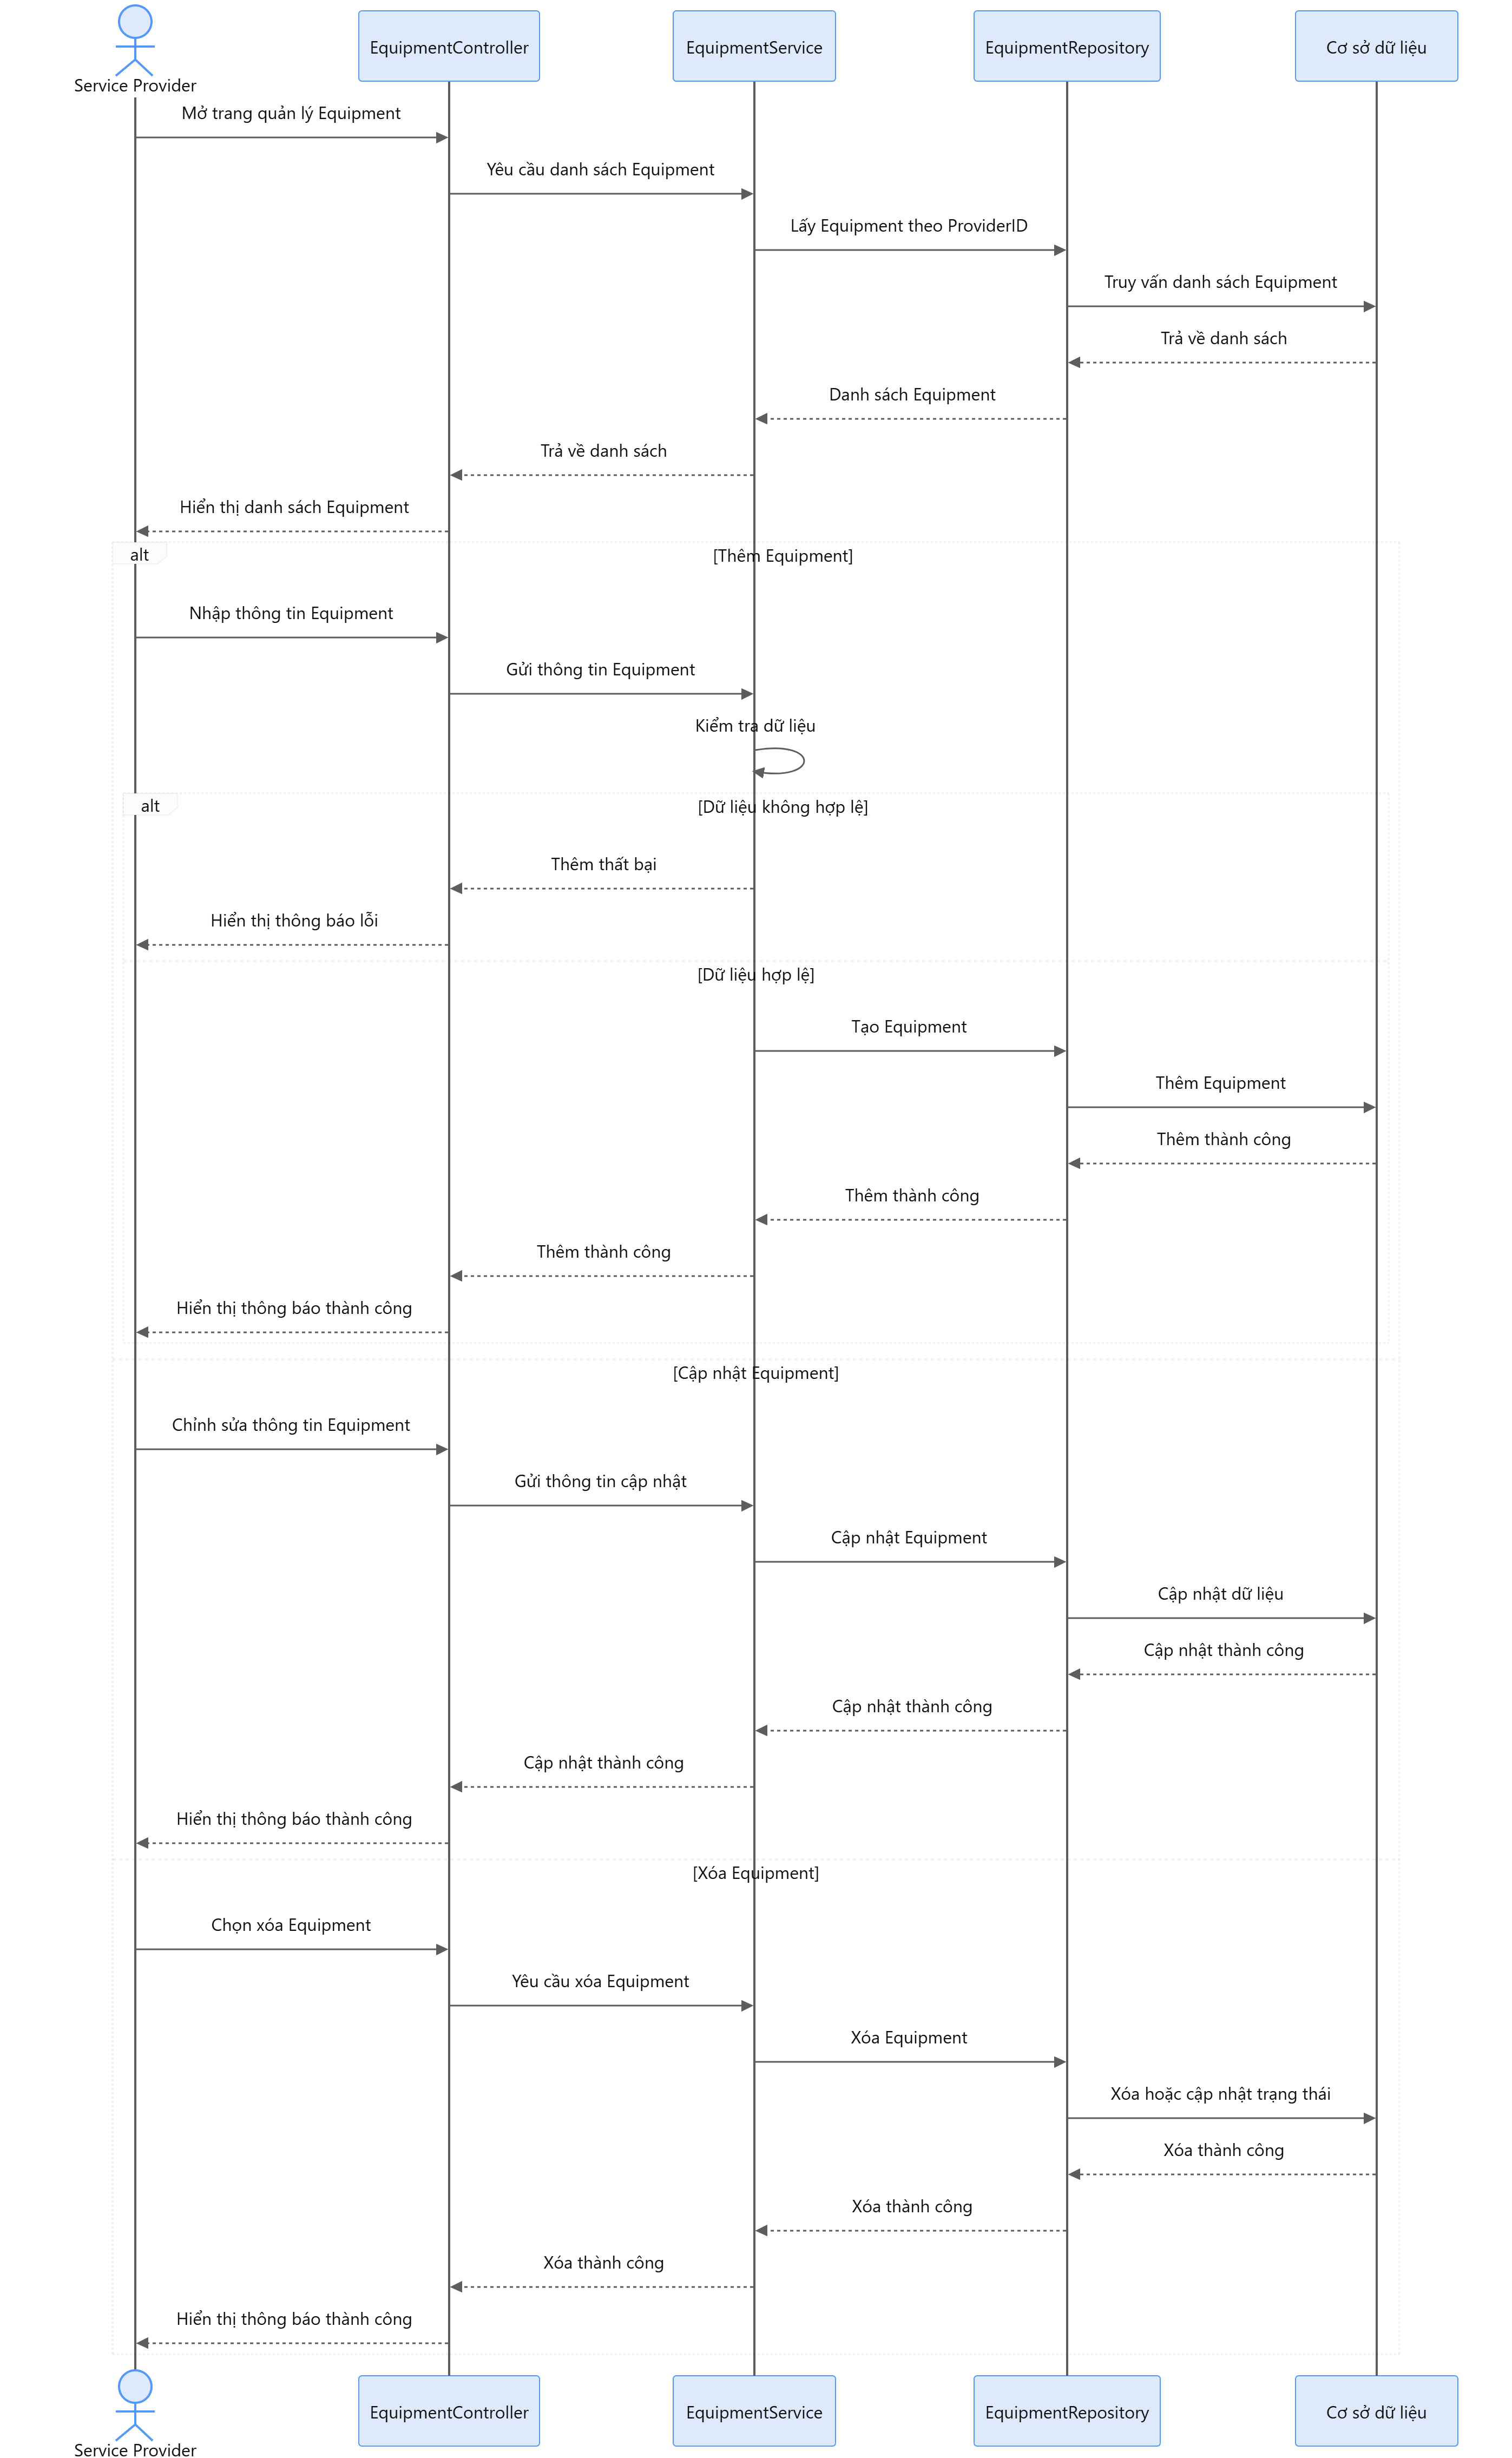
\includegraphics[width=1.1\textwidth]{images/39.png}
\end{figure}


\subsubsection{Quản lý Service Package}

\paragraph{Class Diagram}

\begin{figure}[H]
	\centering
	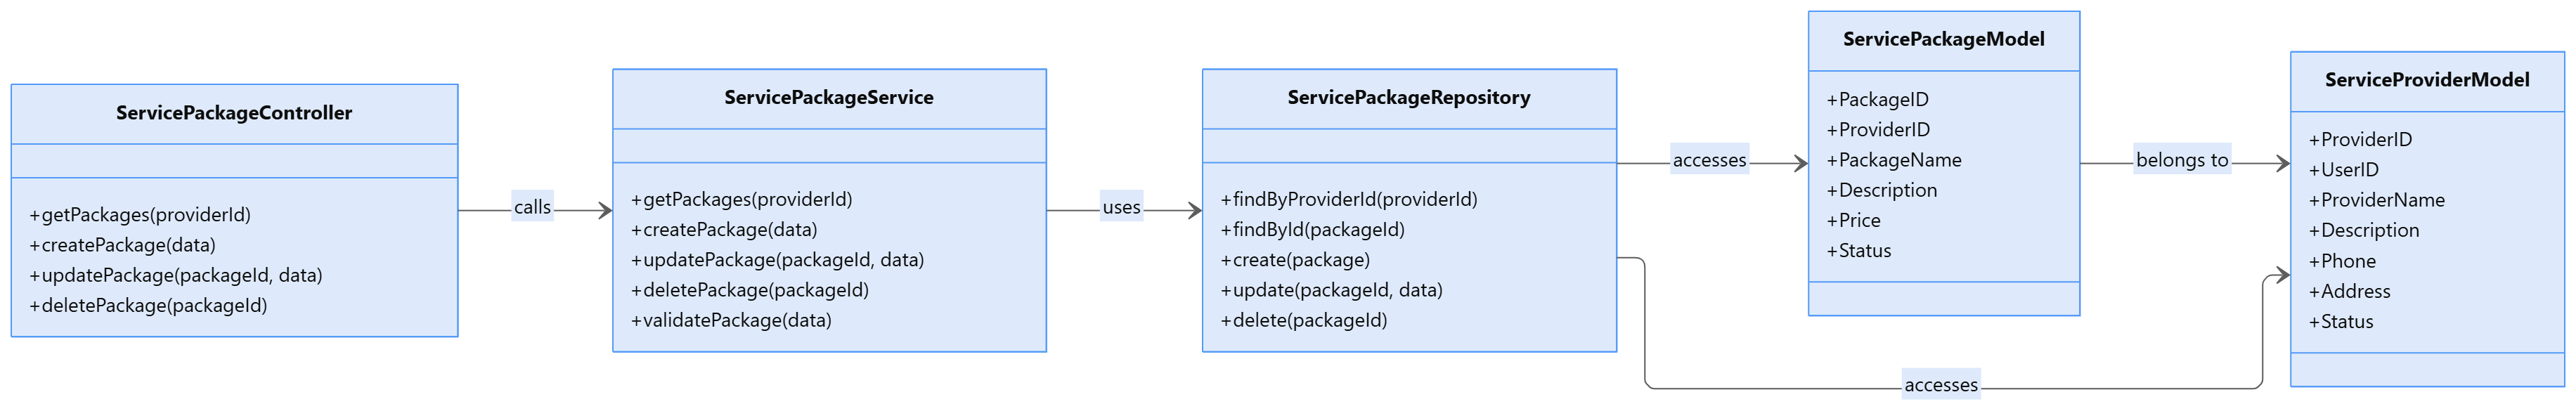
\includegraphics[width=1.1\textwidth]{images/40.png}
\end{figure}

\paragraph{Sequence Diagram}

\begin{figure}[H]
	\centering
	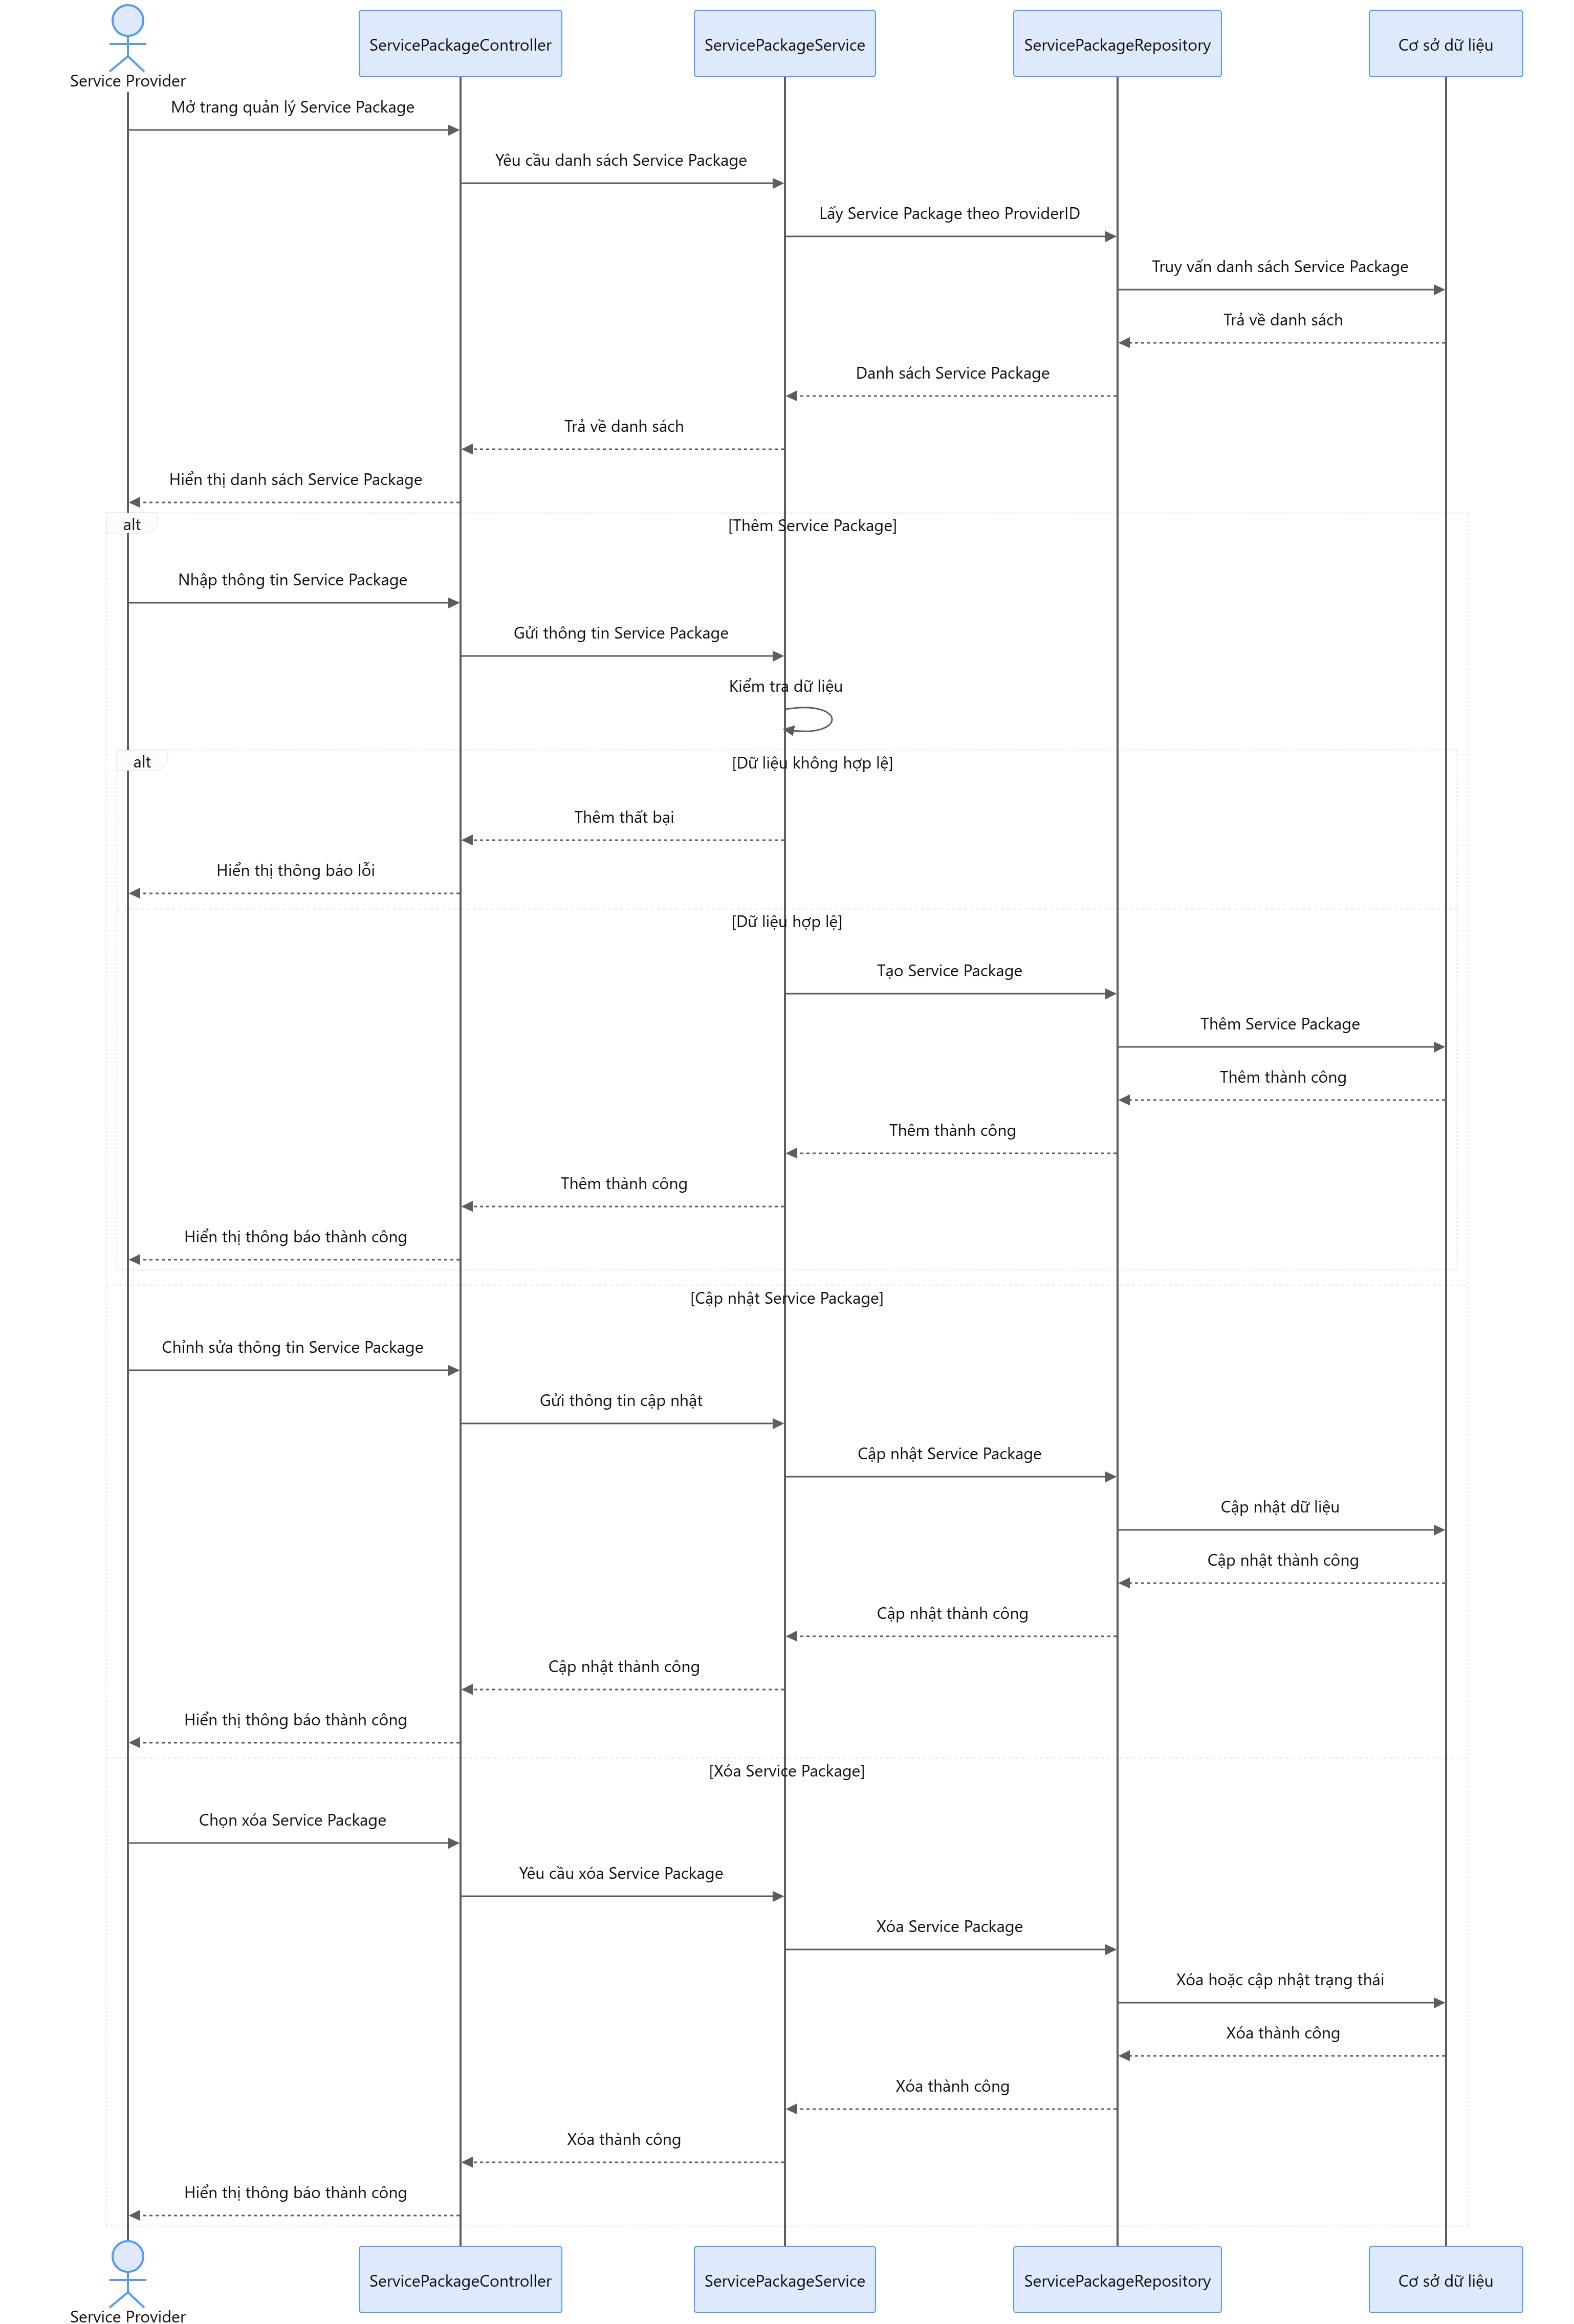
\includegraphics[width=1.1\textwidth]{images/41.png}
\end{figure}


\subsubsection{Quản lý Booking}

\paragraph{Class Diagram}

\begin{figure}[H]
	\centering
	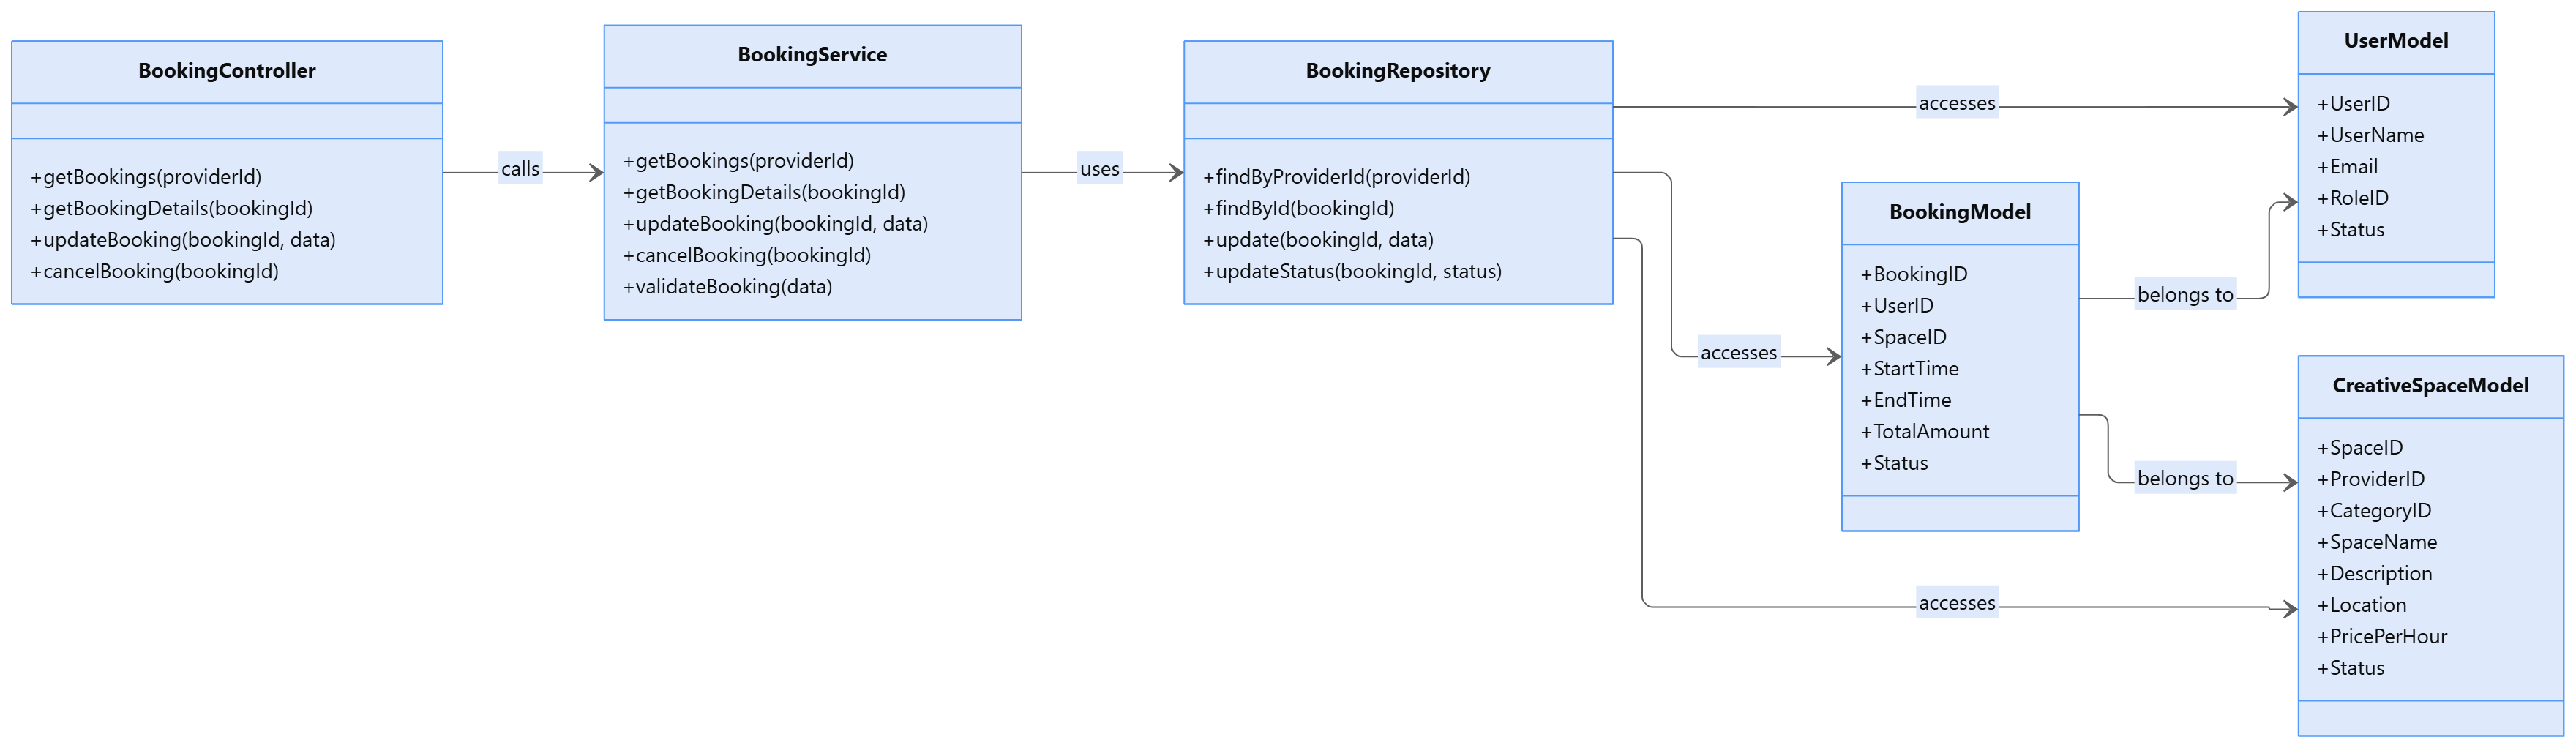
\includegraphics[width=1.1\textwidth]{images/42.png}
\end{figure}

\paragraph{Sequence Diagram}

\begin{figure}[H]
	\centering
	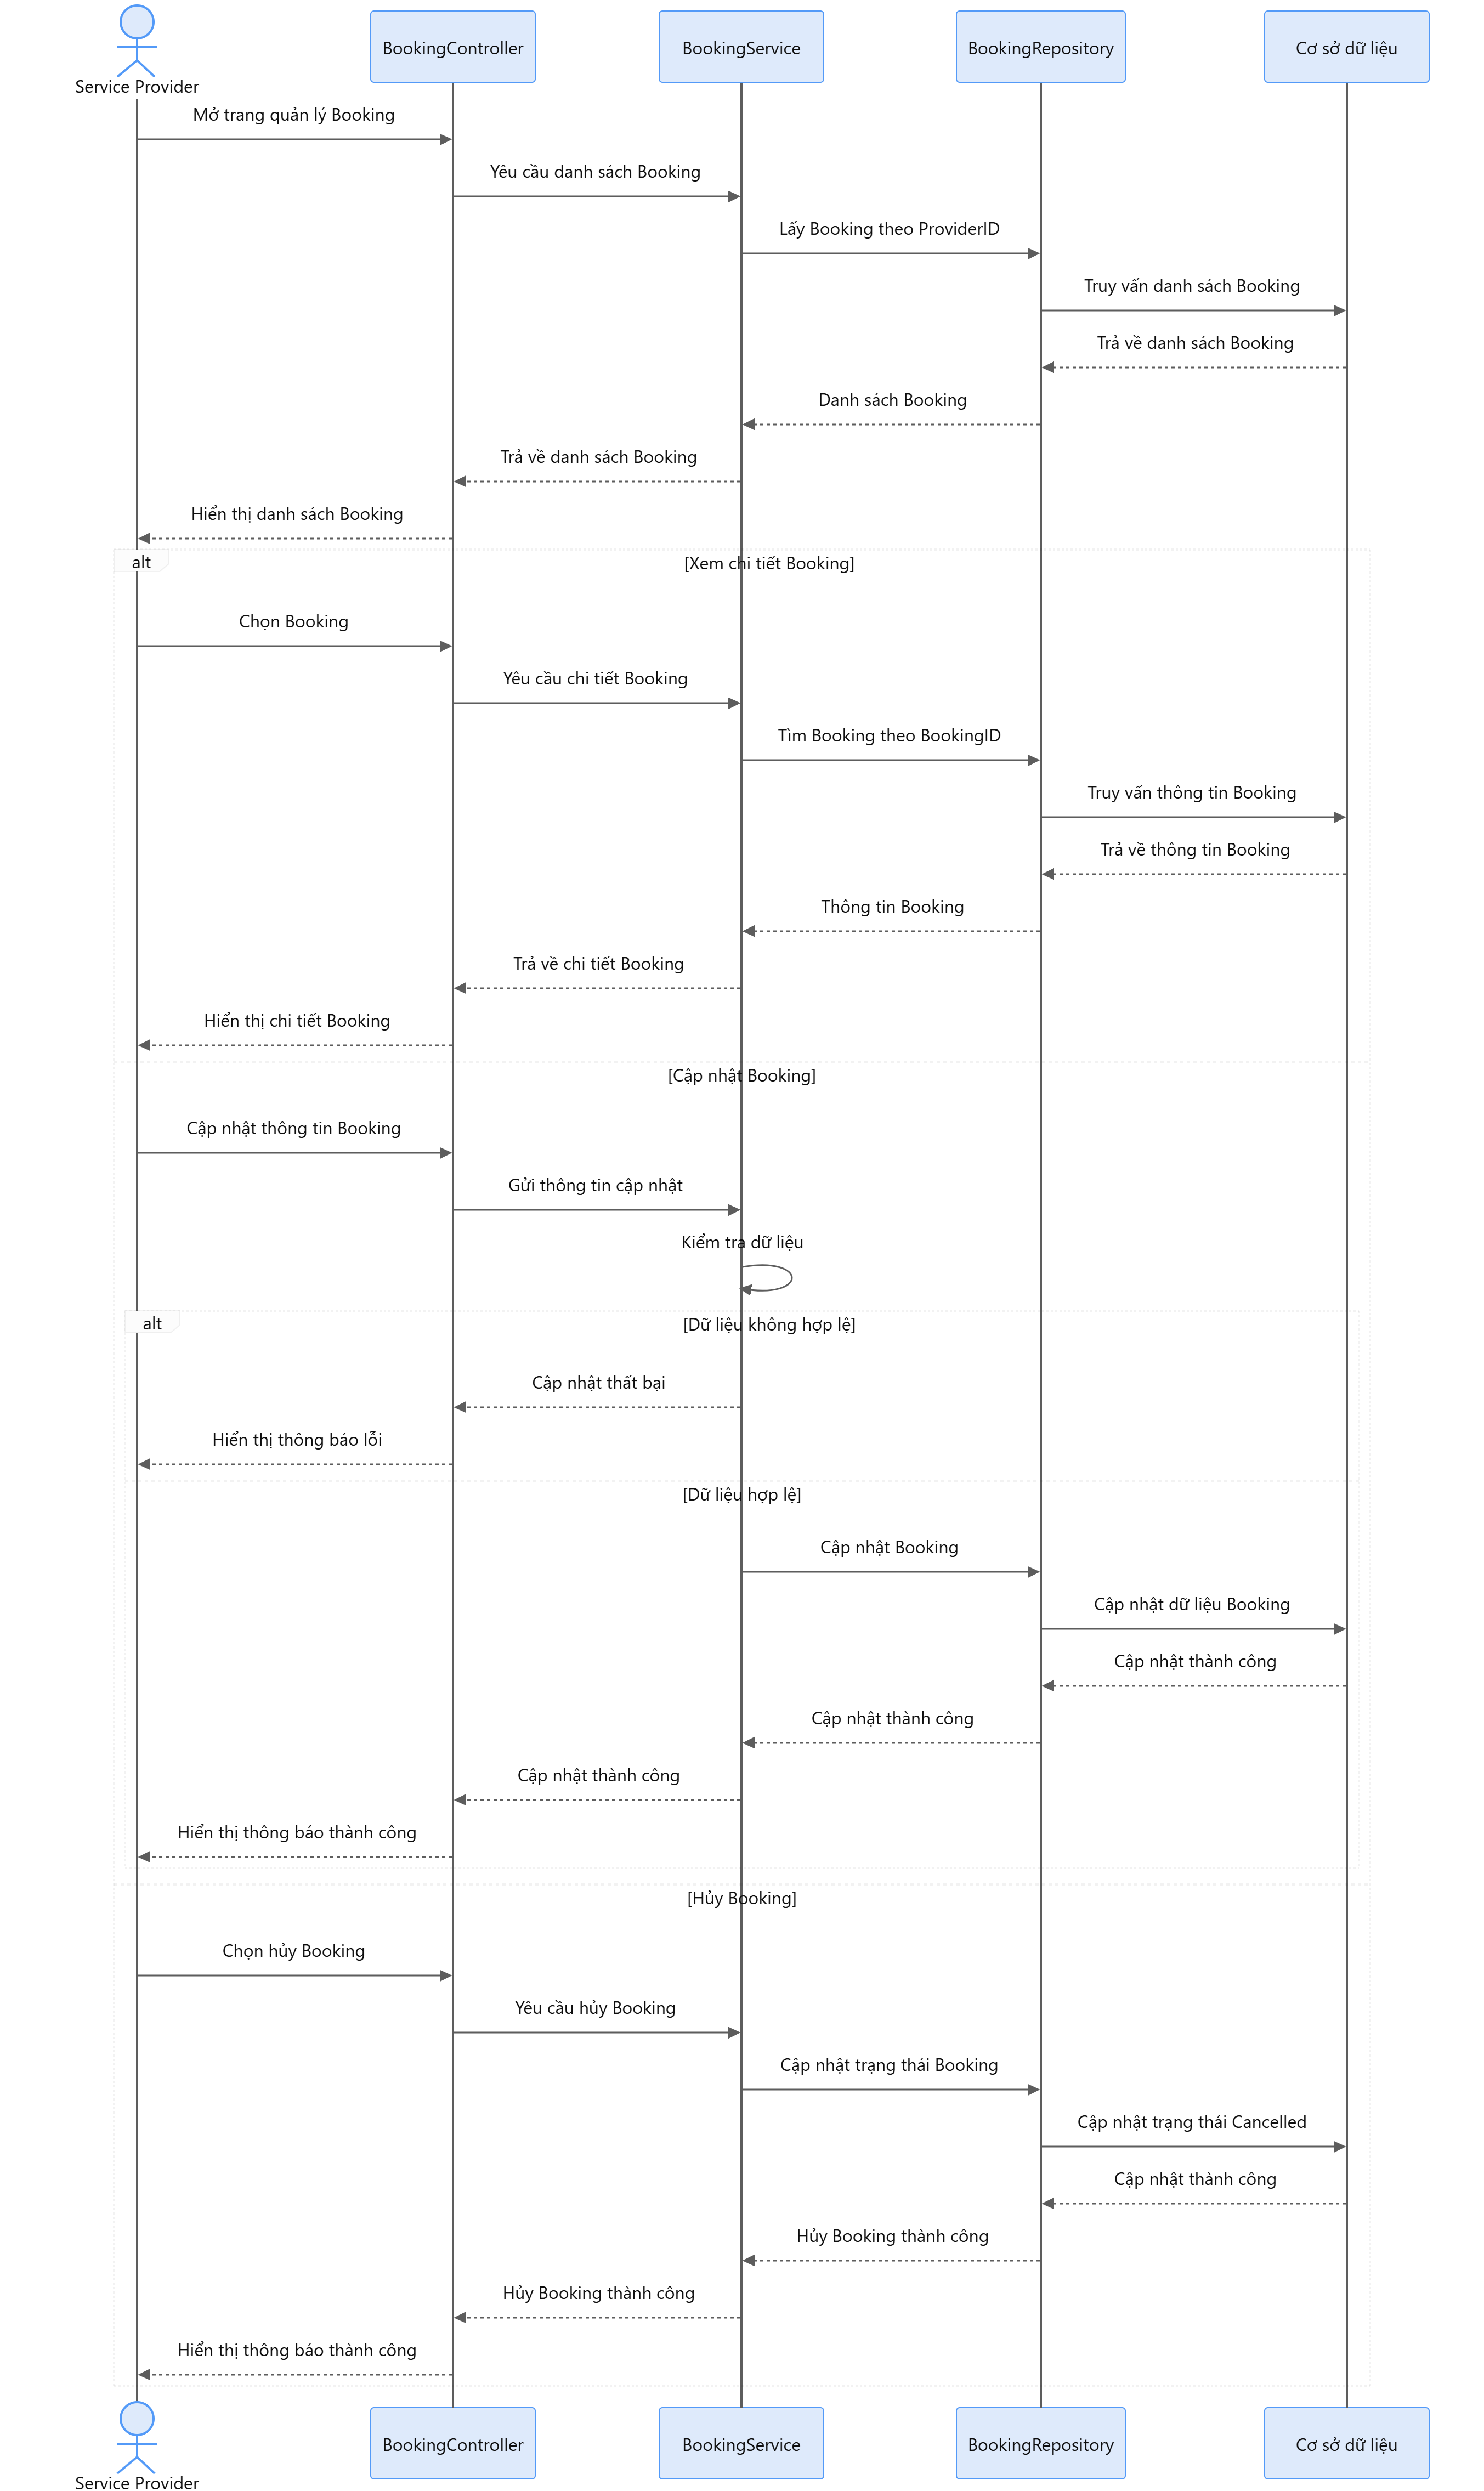
\includegraphics[width=1.1\textwidth]{images/43.png}
\end{figure}


\subsubsection{Xác nhận/Từ chối Booking}

\paragraph{Class Diagram}

\begin{figure}[H]
	\centering
	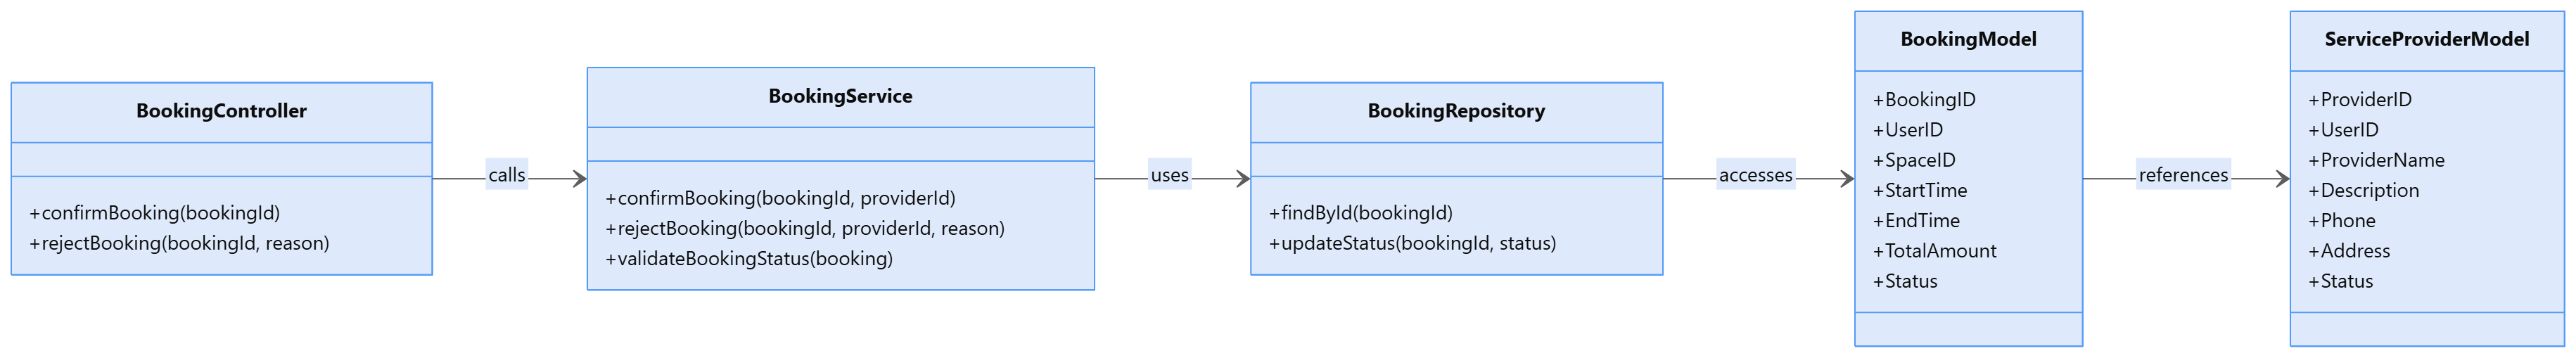
\includegraphics[width=1.1\textwidth]{images/44.png}
\end{figure}

\paragraph{Sequence Diagram}

\begin{figure}[H]
	\centering
	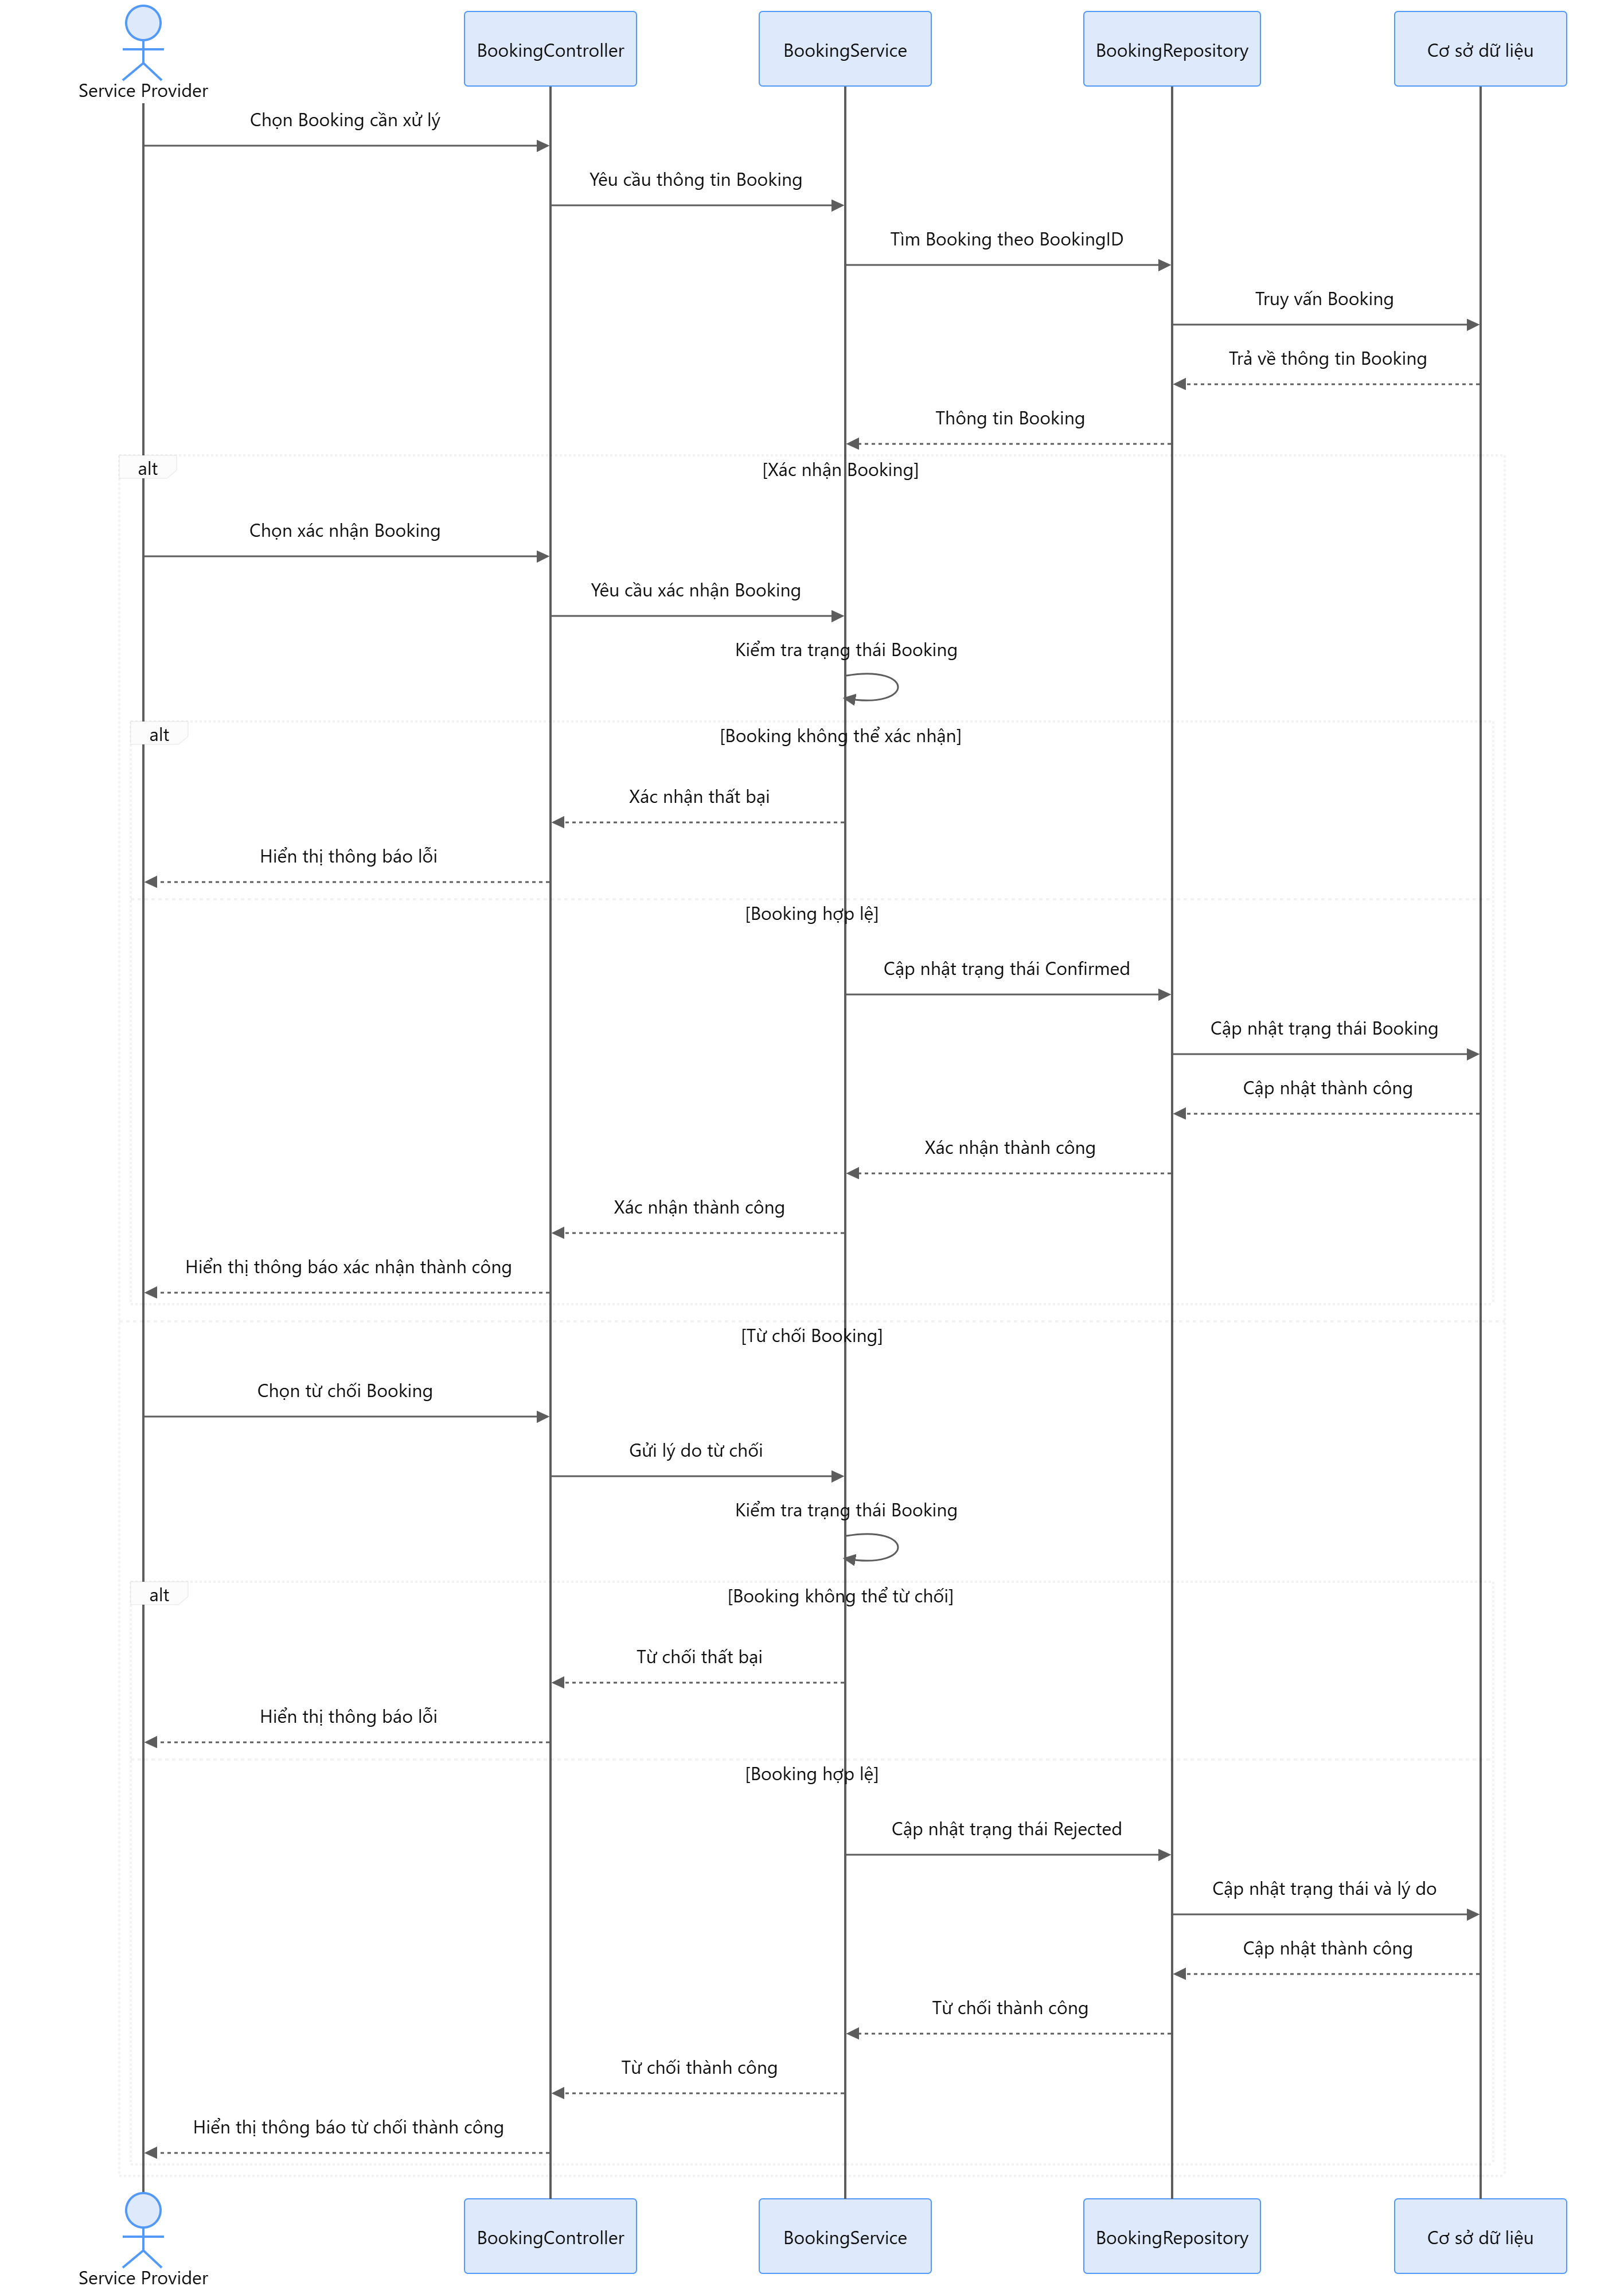
\includegraphics[width=1.1\textwidth]{images/45.png}
\end{figure}


\subsubsection{Quản lý Workshop}

\paragraph{Class Diagram}

\begin{figure}[H]
	\centering
	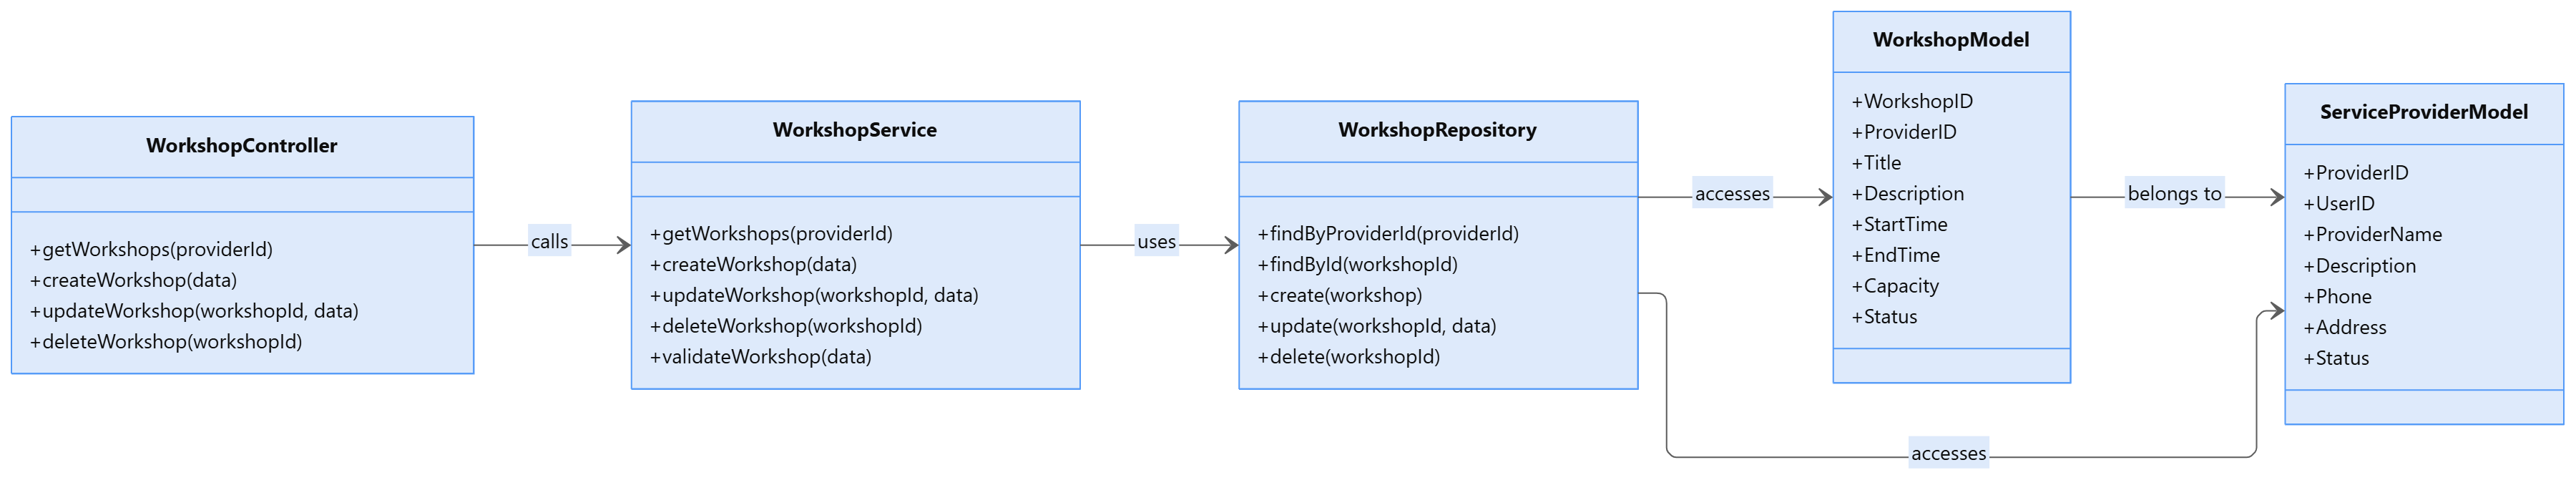
\includegraphics[width=1.1\textwidth]{images/46.png}
\end{figure}

\paragraph{Sequence Diagram}

\begin{figure}[H]
	\centering
	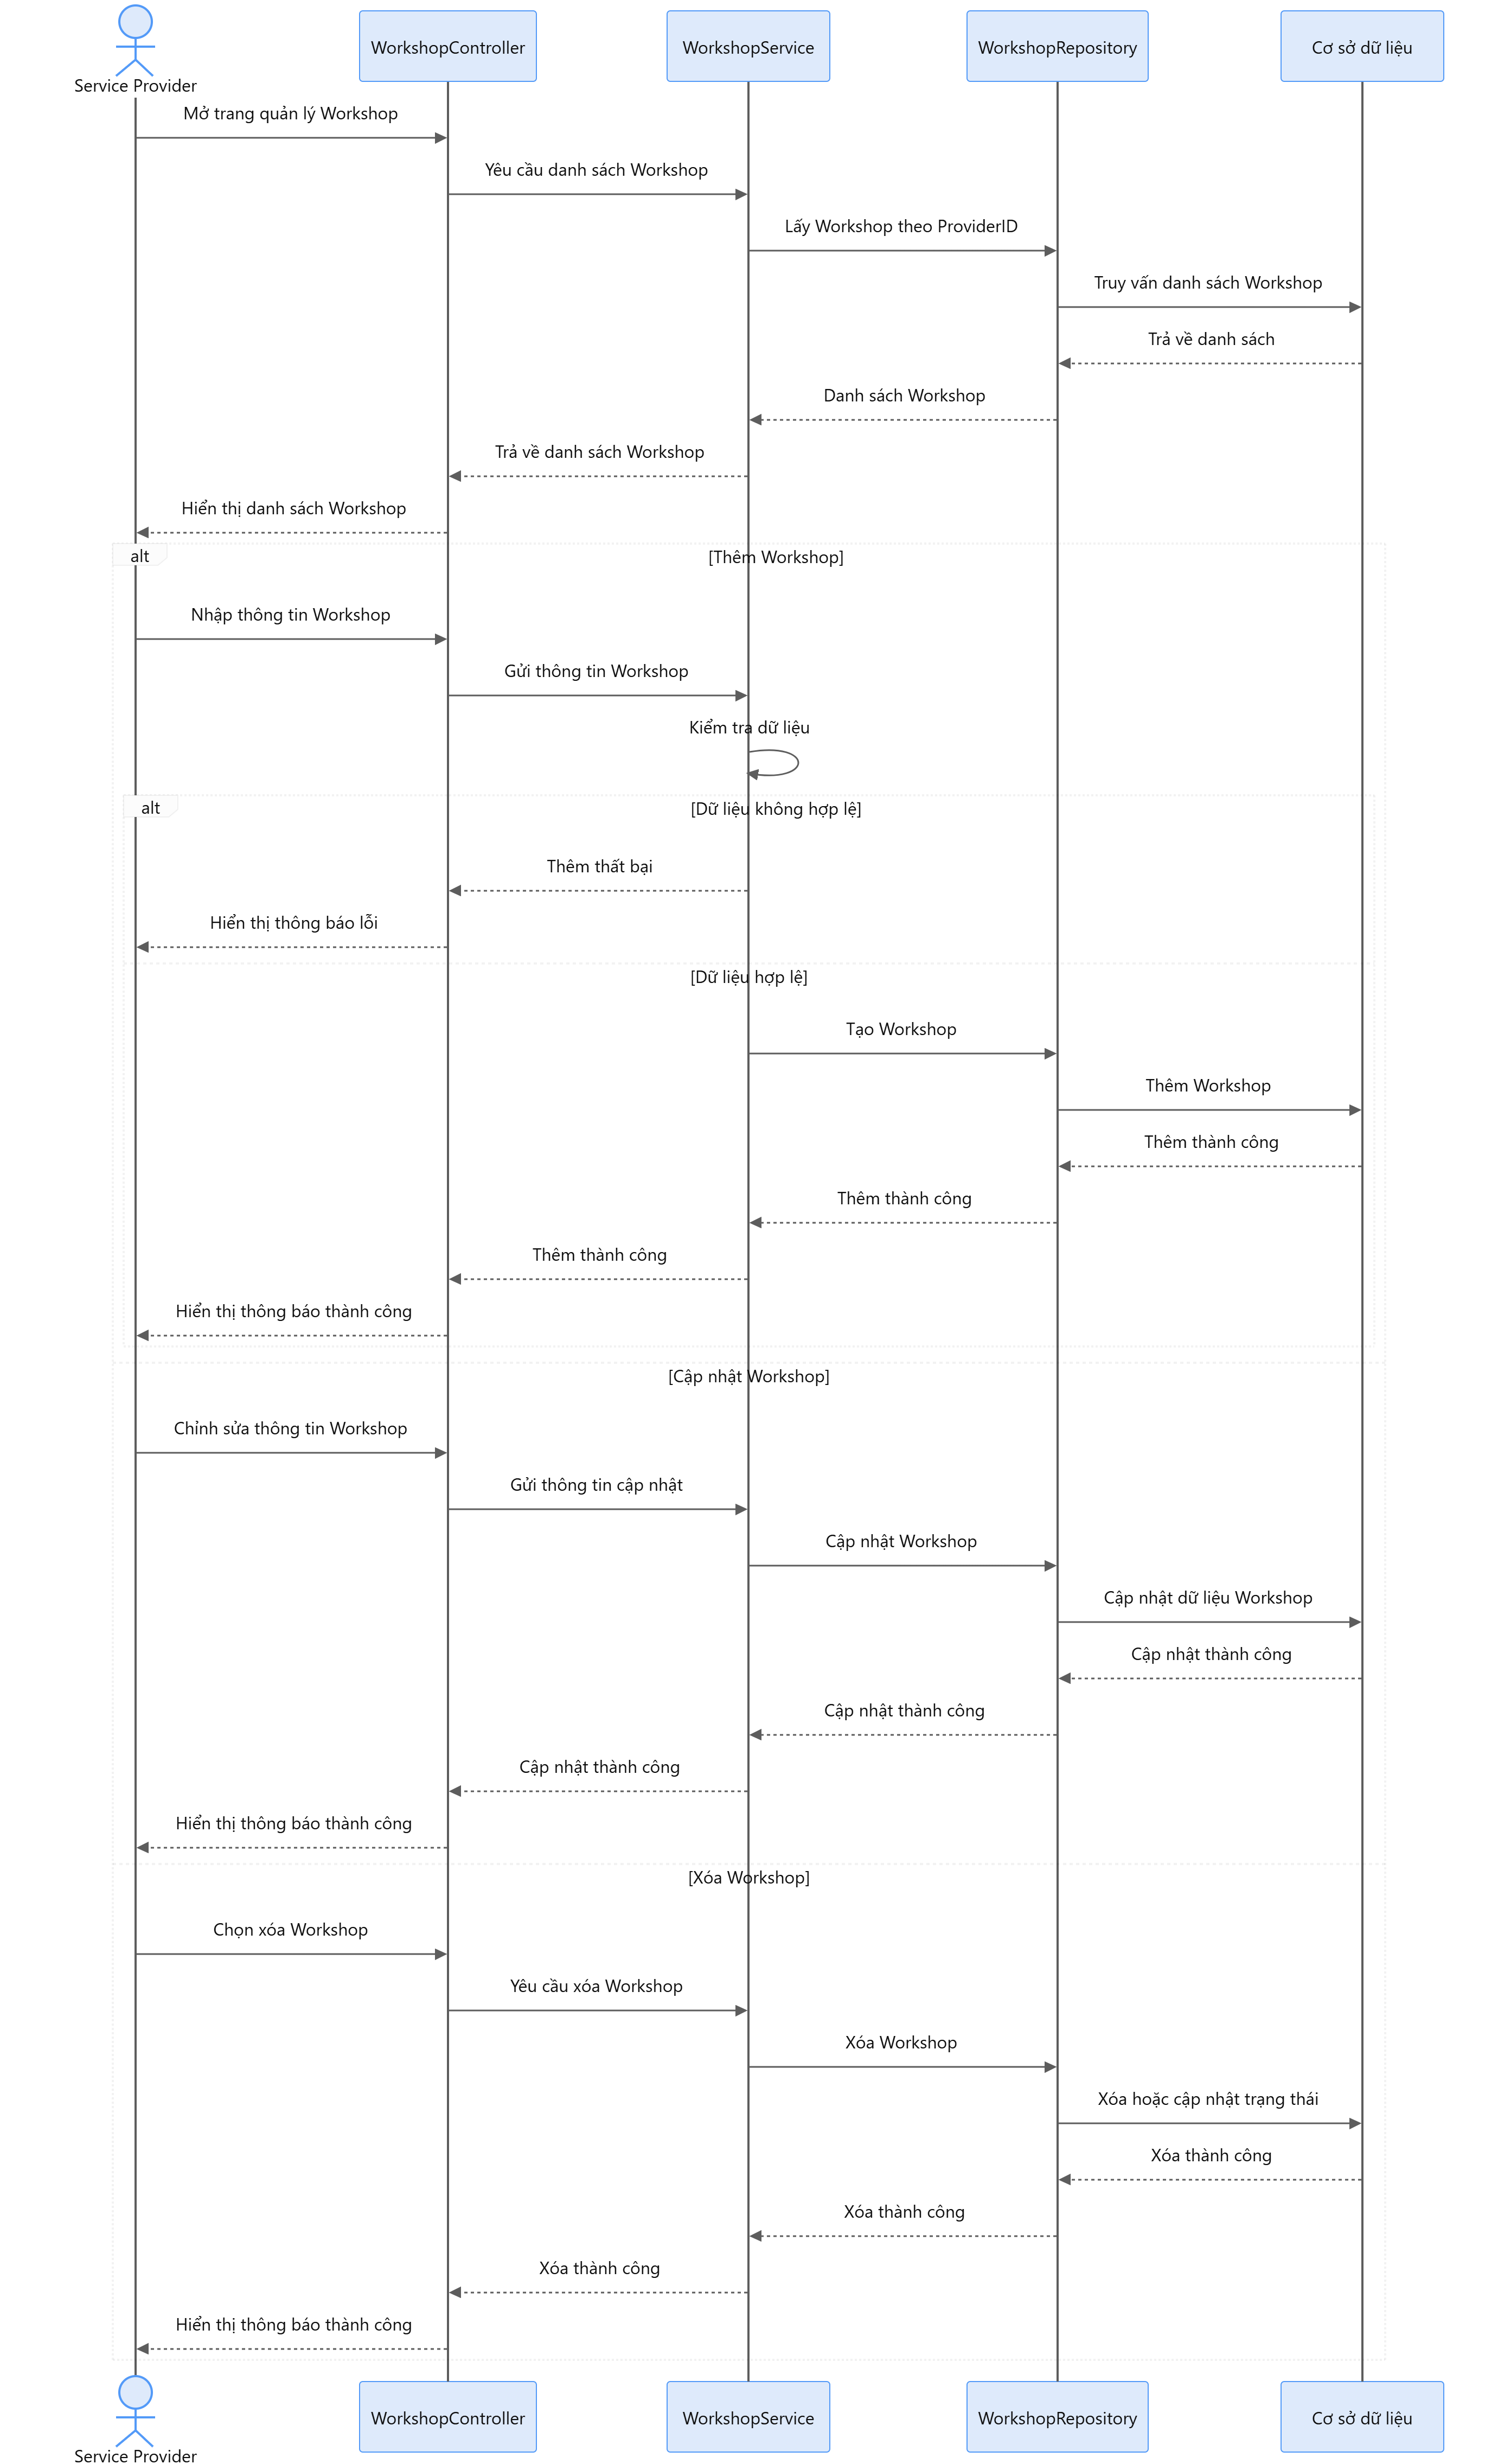
\includegraphics[width=1.1\textwidth]{images/47.png}
\end{figure}


% =========================================================
% 3.8 Administrator Management Module
% =========================================================

\subsection{Administrator Management Module}

\subsubsection{Quản lý người dùng}

\paragraph{Class Diagram}

\begin{figure}[H]
	\centering
	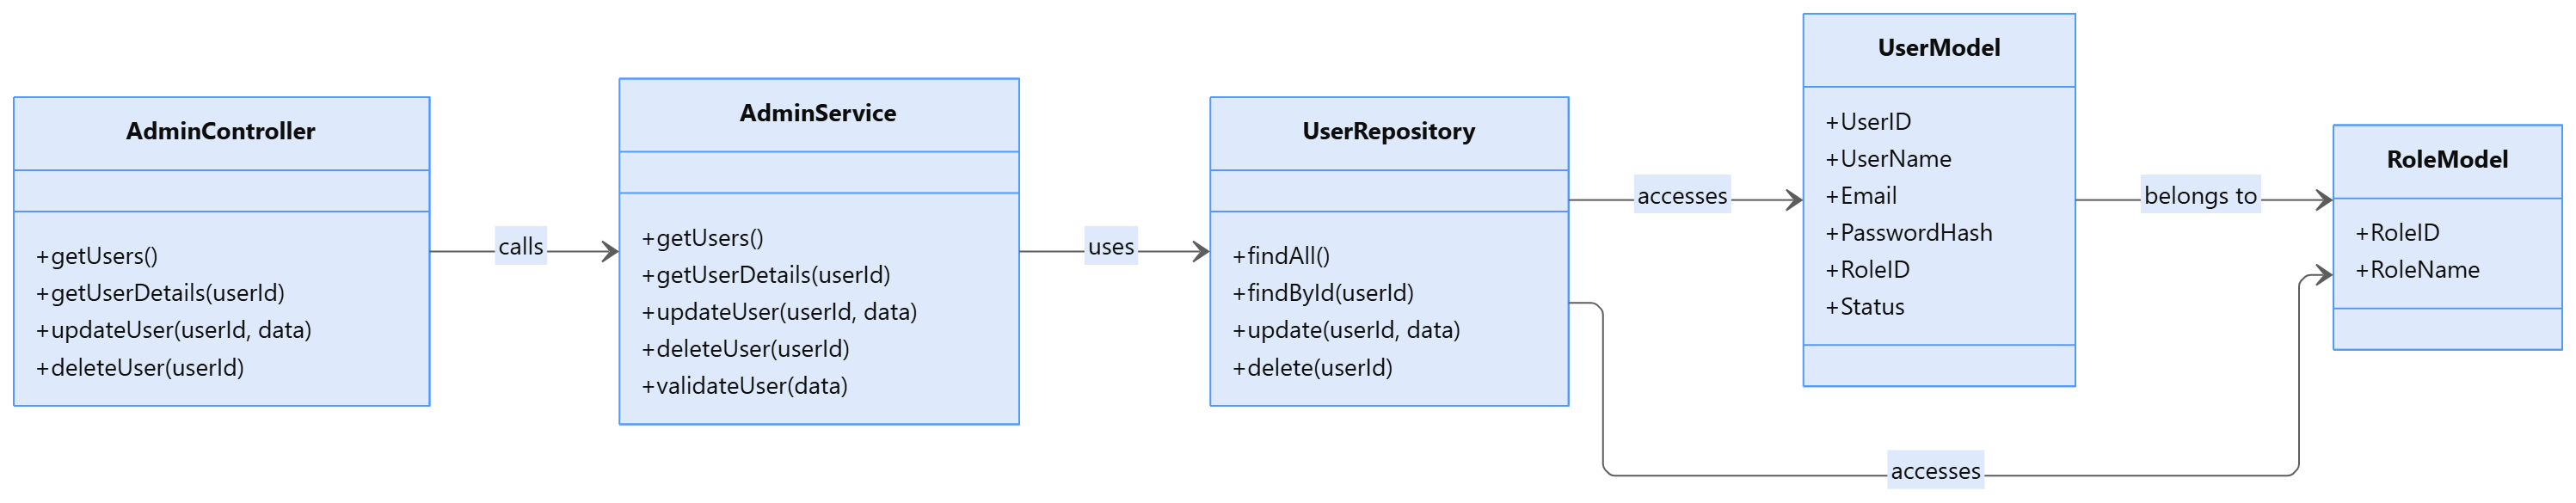
\includegraphics[width=1.1\textwidth]{images/48.png}
\end{figure}

\paragraph{Sequence Diagram}

\begin{figure}[H]
	\centering
	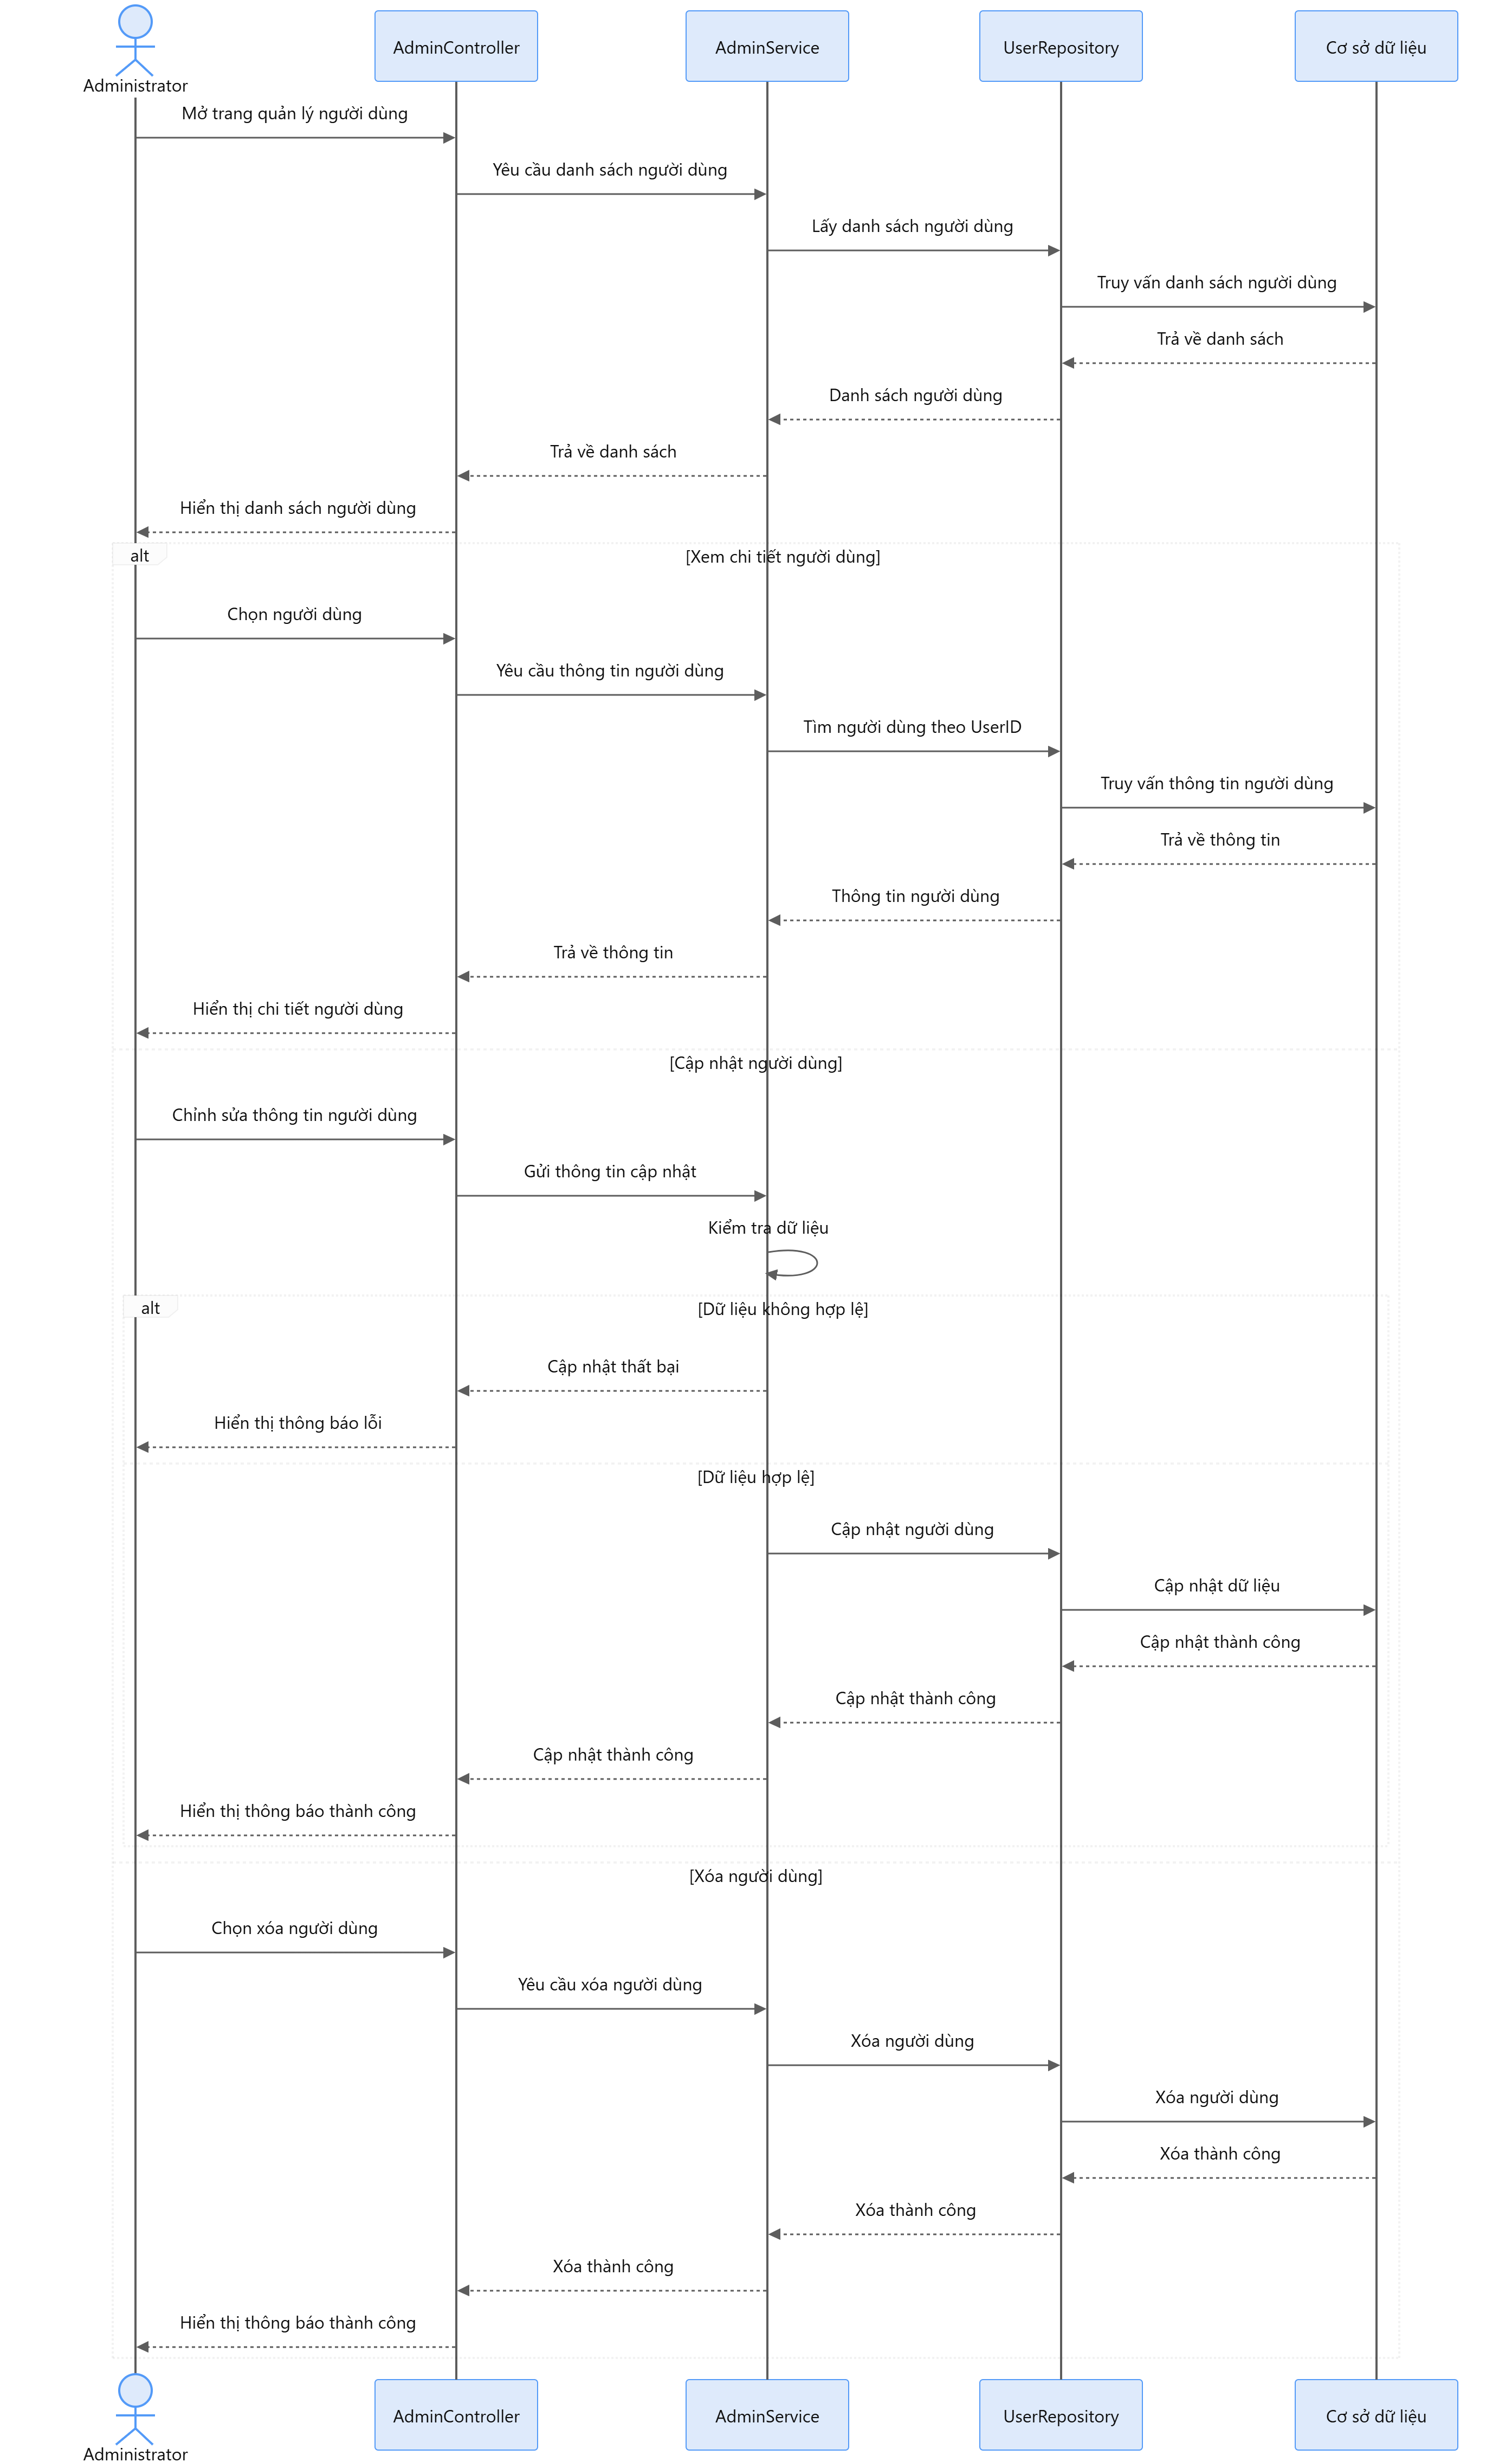
\includegraphics[width=1.1\textwidth]{images/49.png}
\end{figure}


\subsubsection{Quản lý Service Provider}

\paragraph{Class Diagram}

\begin{figure}[H]
	\centering
	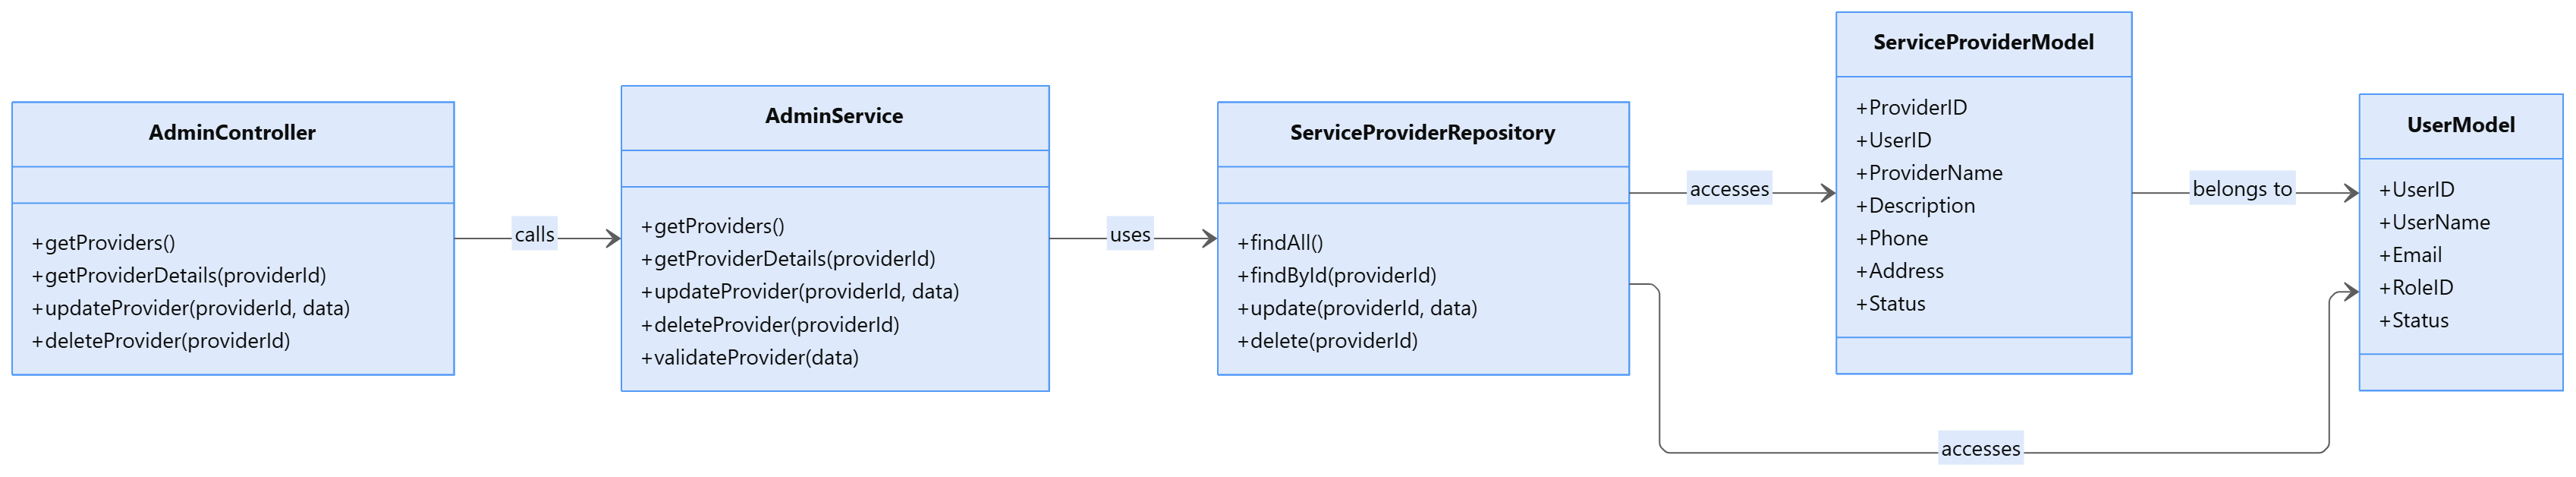
\includegraphics[width=1.1\textwidth]{images/50.png}
\end{figure}

\paragraph{Sequence Diagram}

\begin{figure}[H]
	\centering
	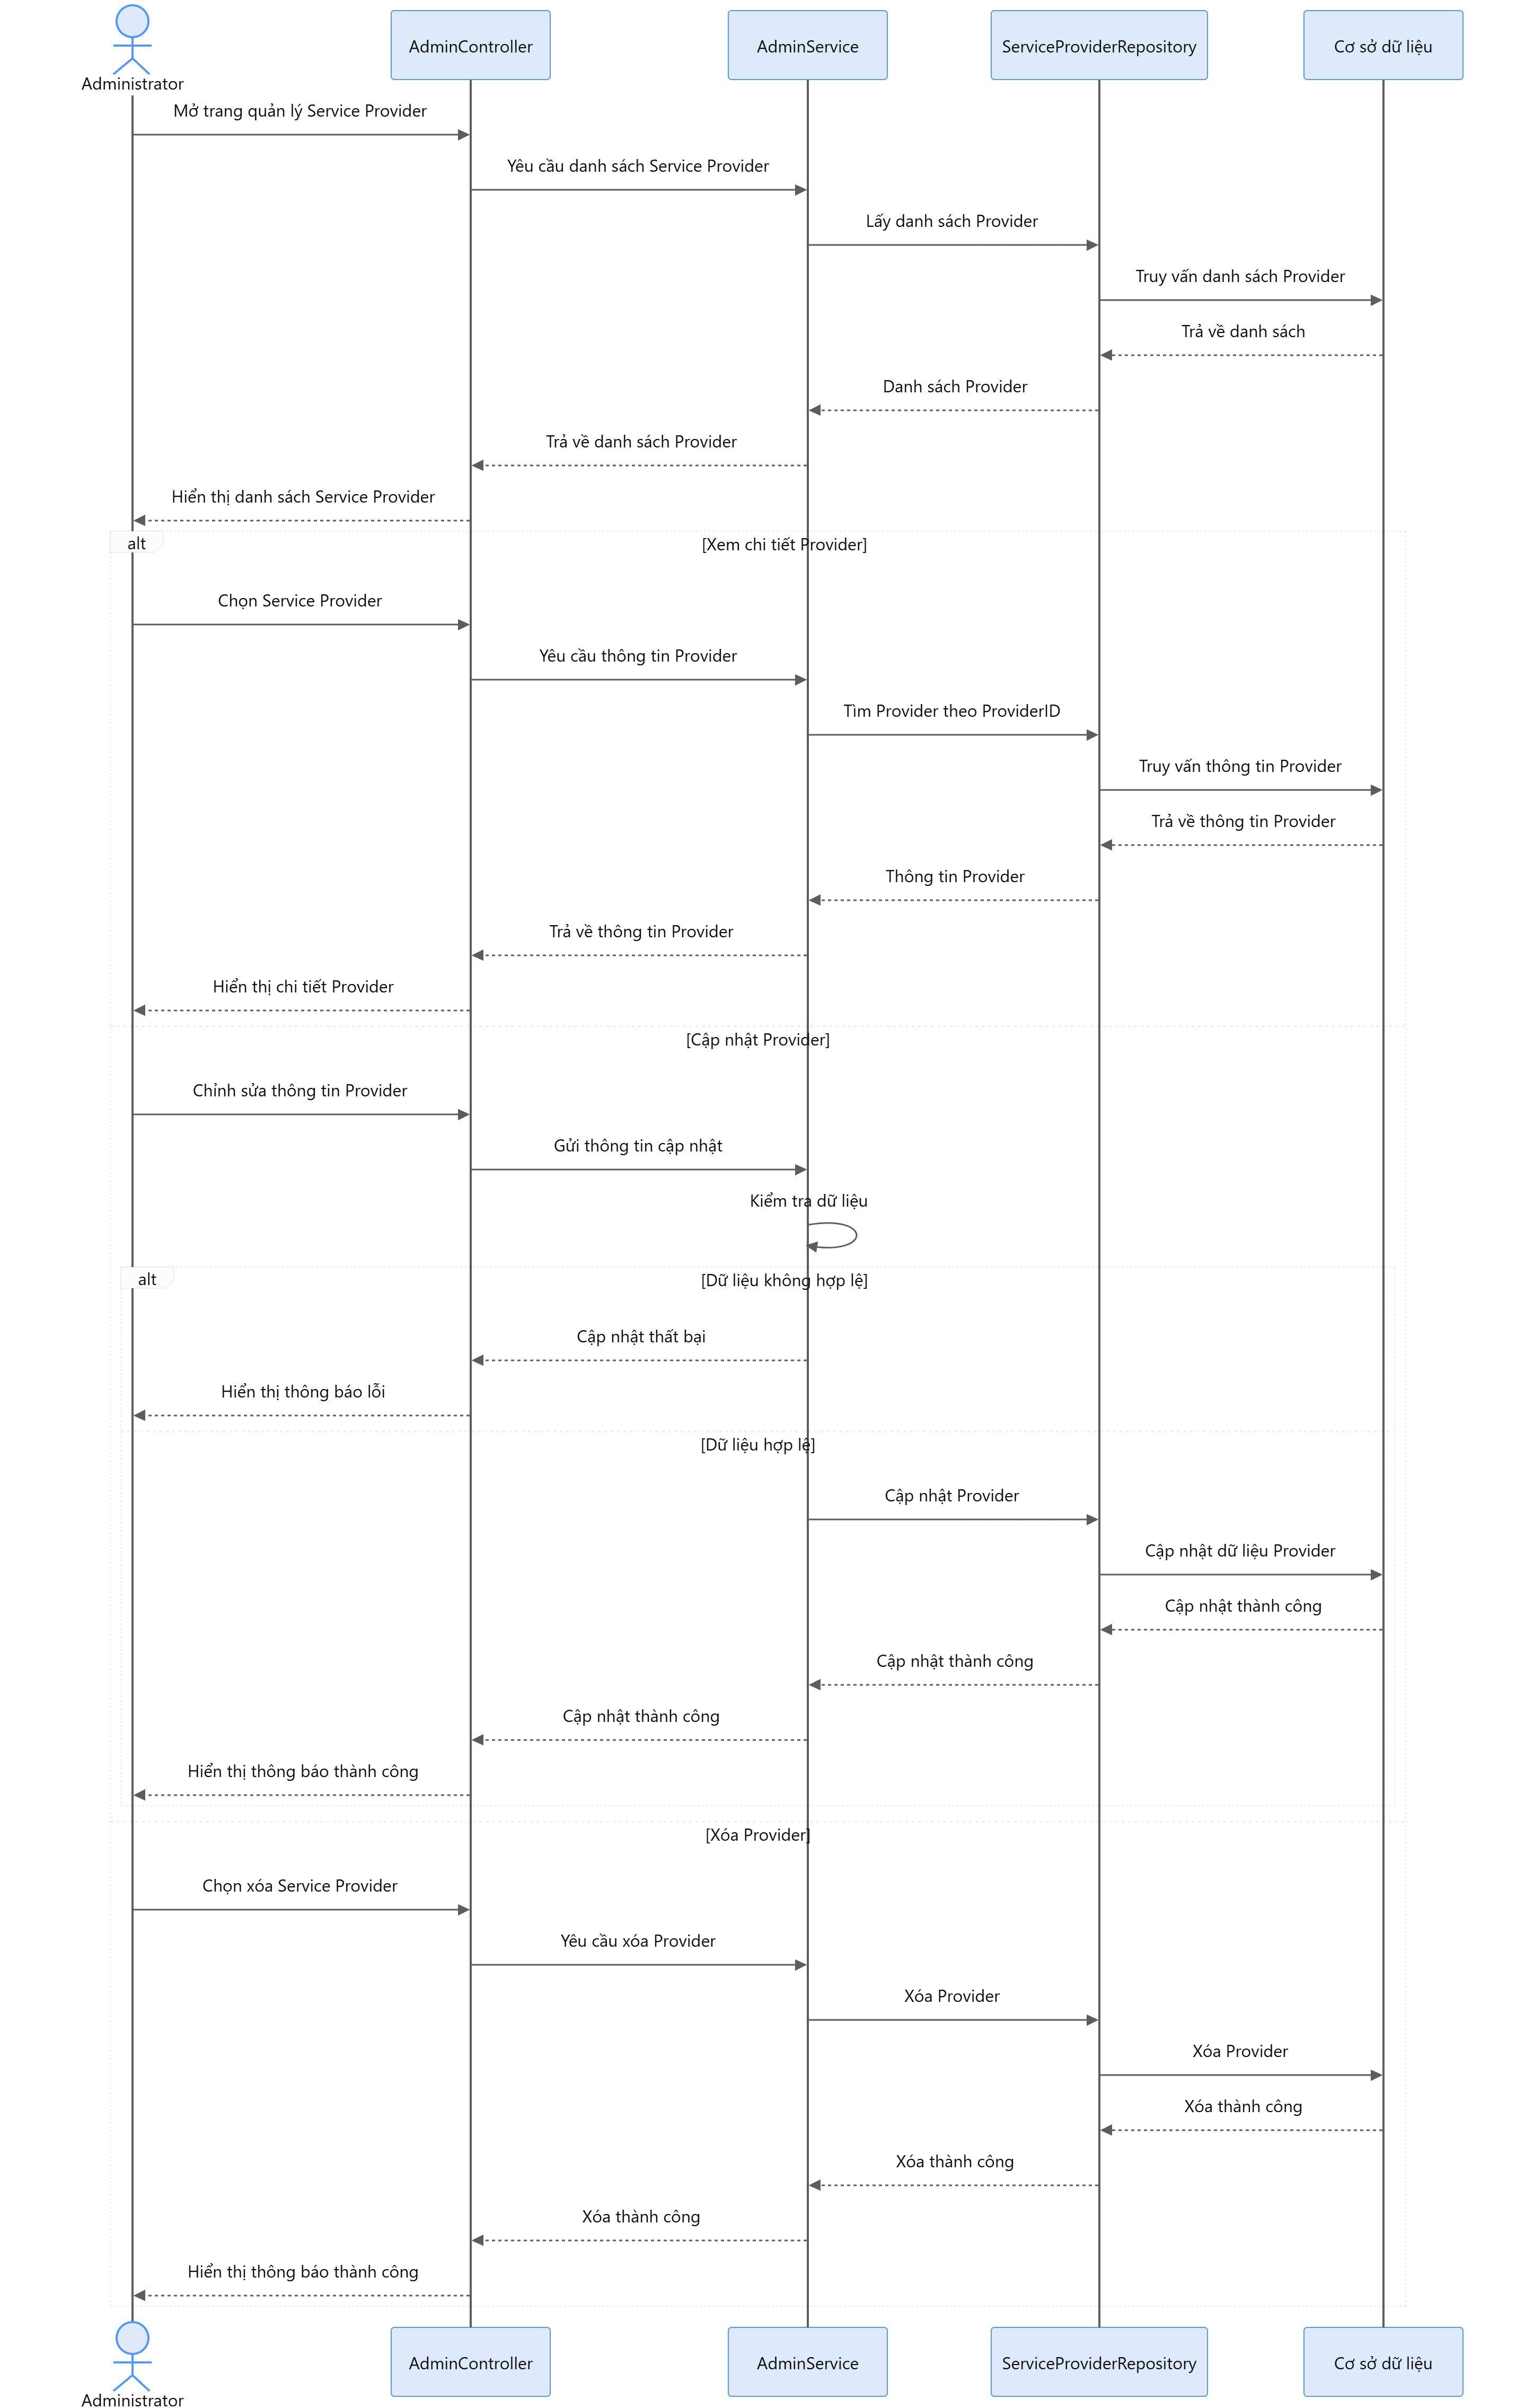
\includegraphics[width=1.1\textwidth]{images/51.png}
\end{figure}


\subsubsection{Phê duyệt Service Provider}

\paragraph{Class Diagram}

\begin{figure}[H]
	\centering
	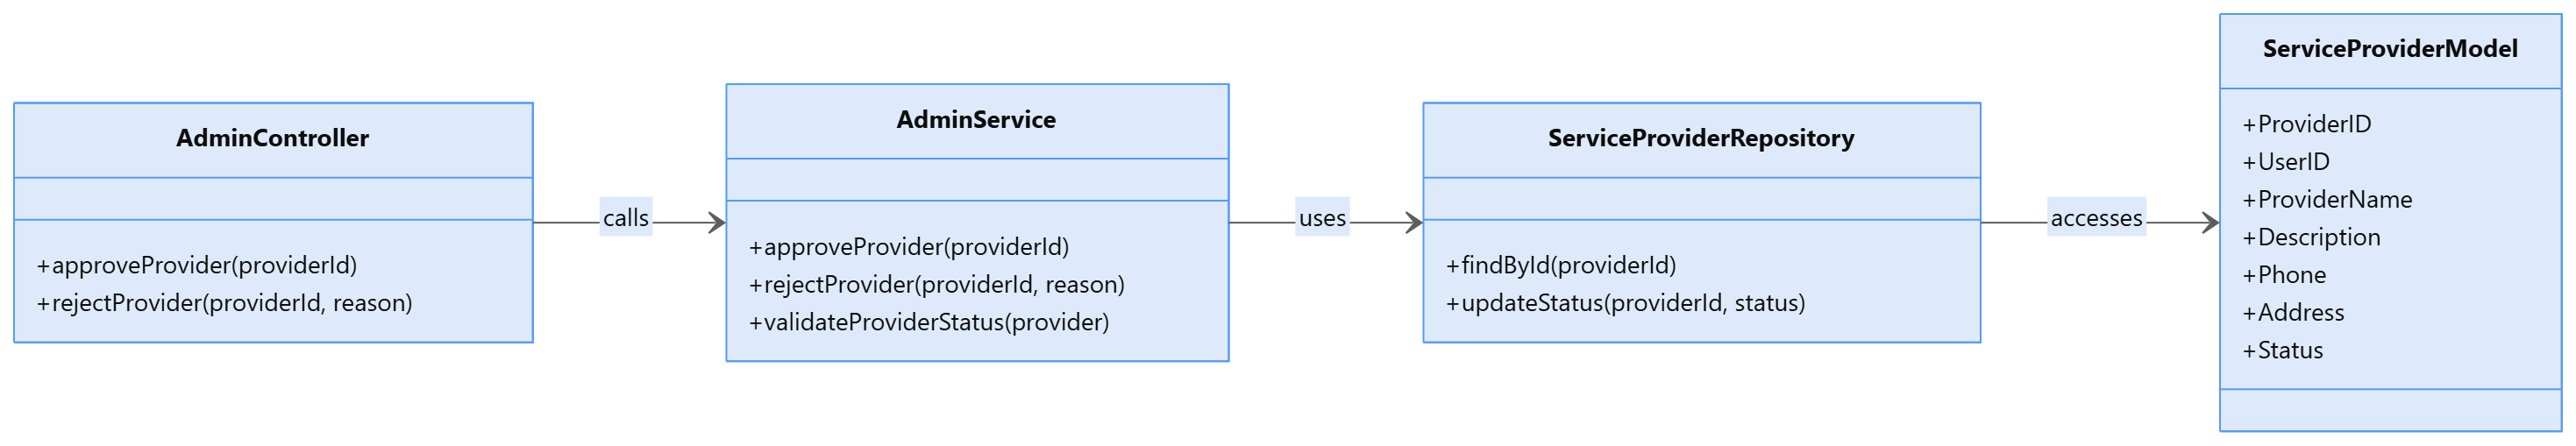
\includegraphics[width=1.1\textwidth]{images/52.png}
\end{figure}

\paragraph{Sequence Diagram}

\begin{figure}[H]
	\centering
	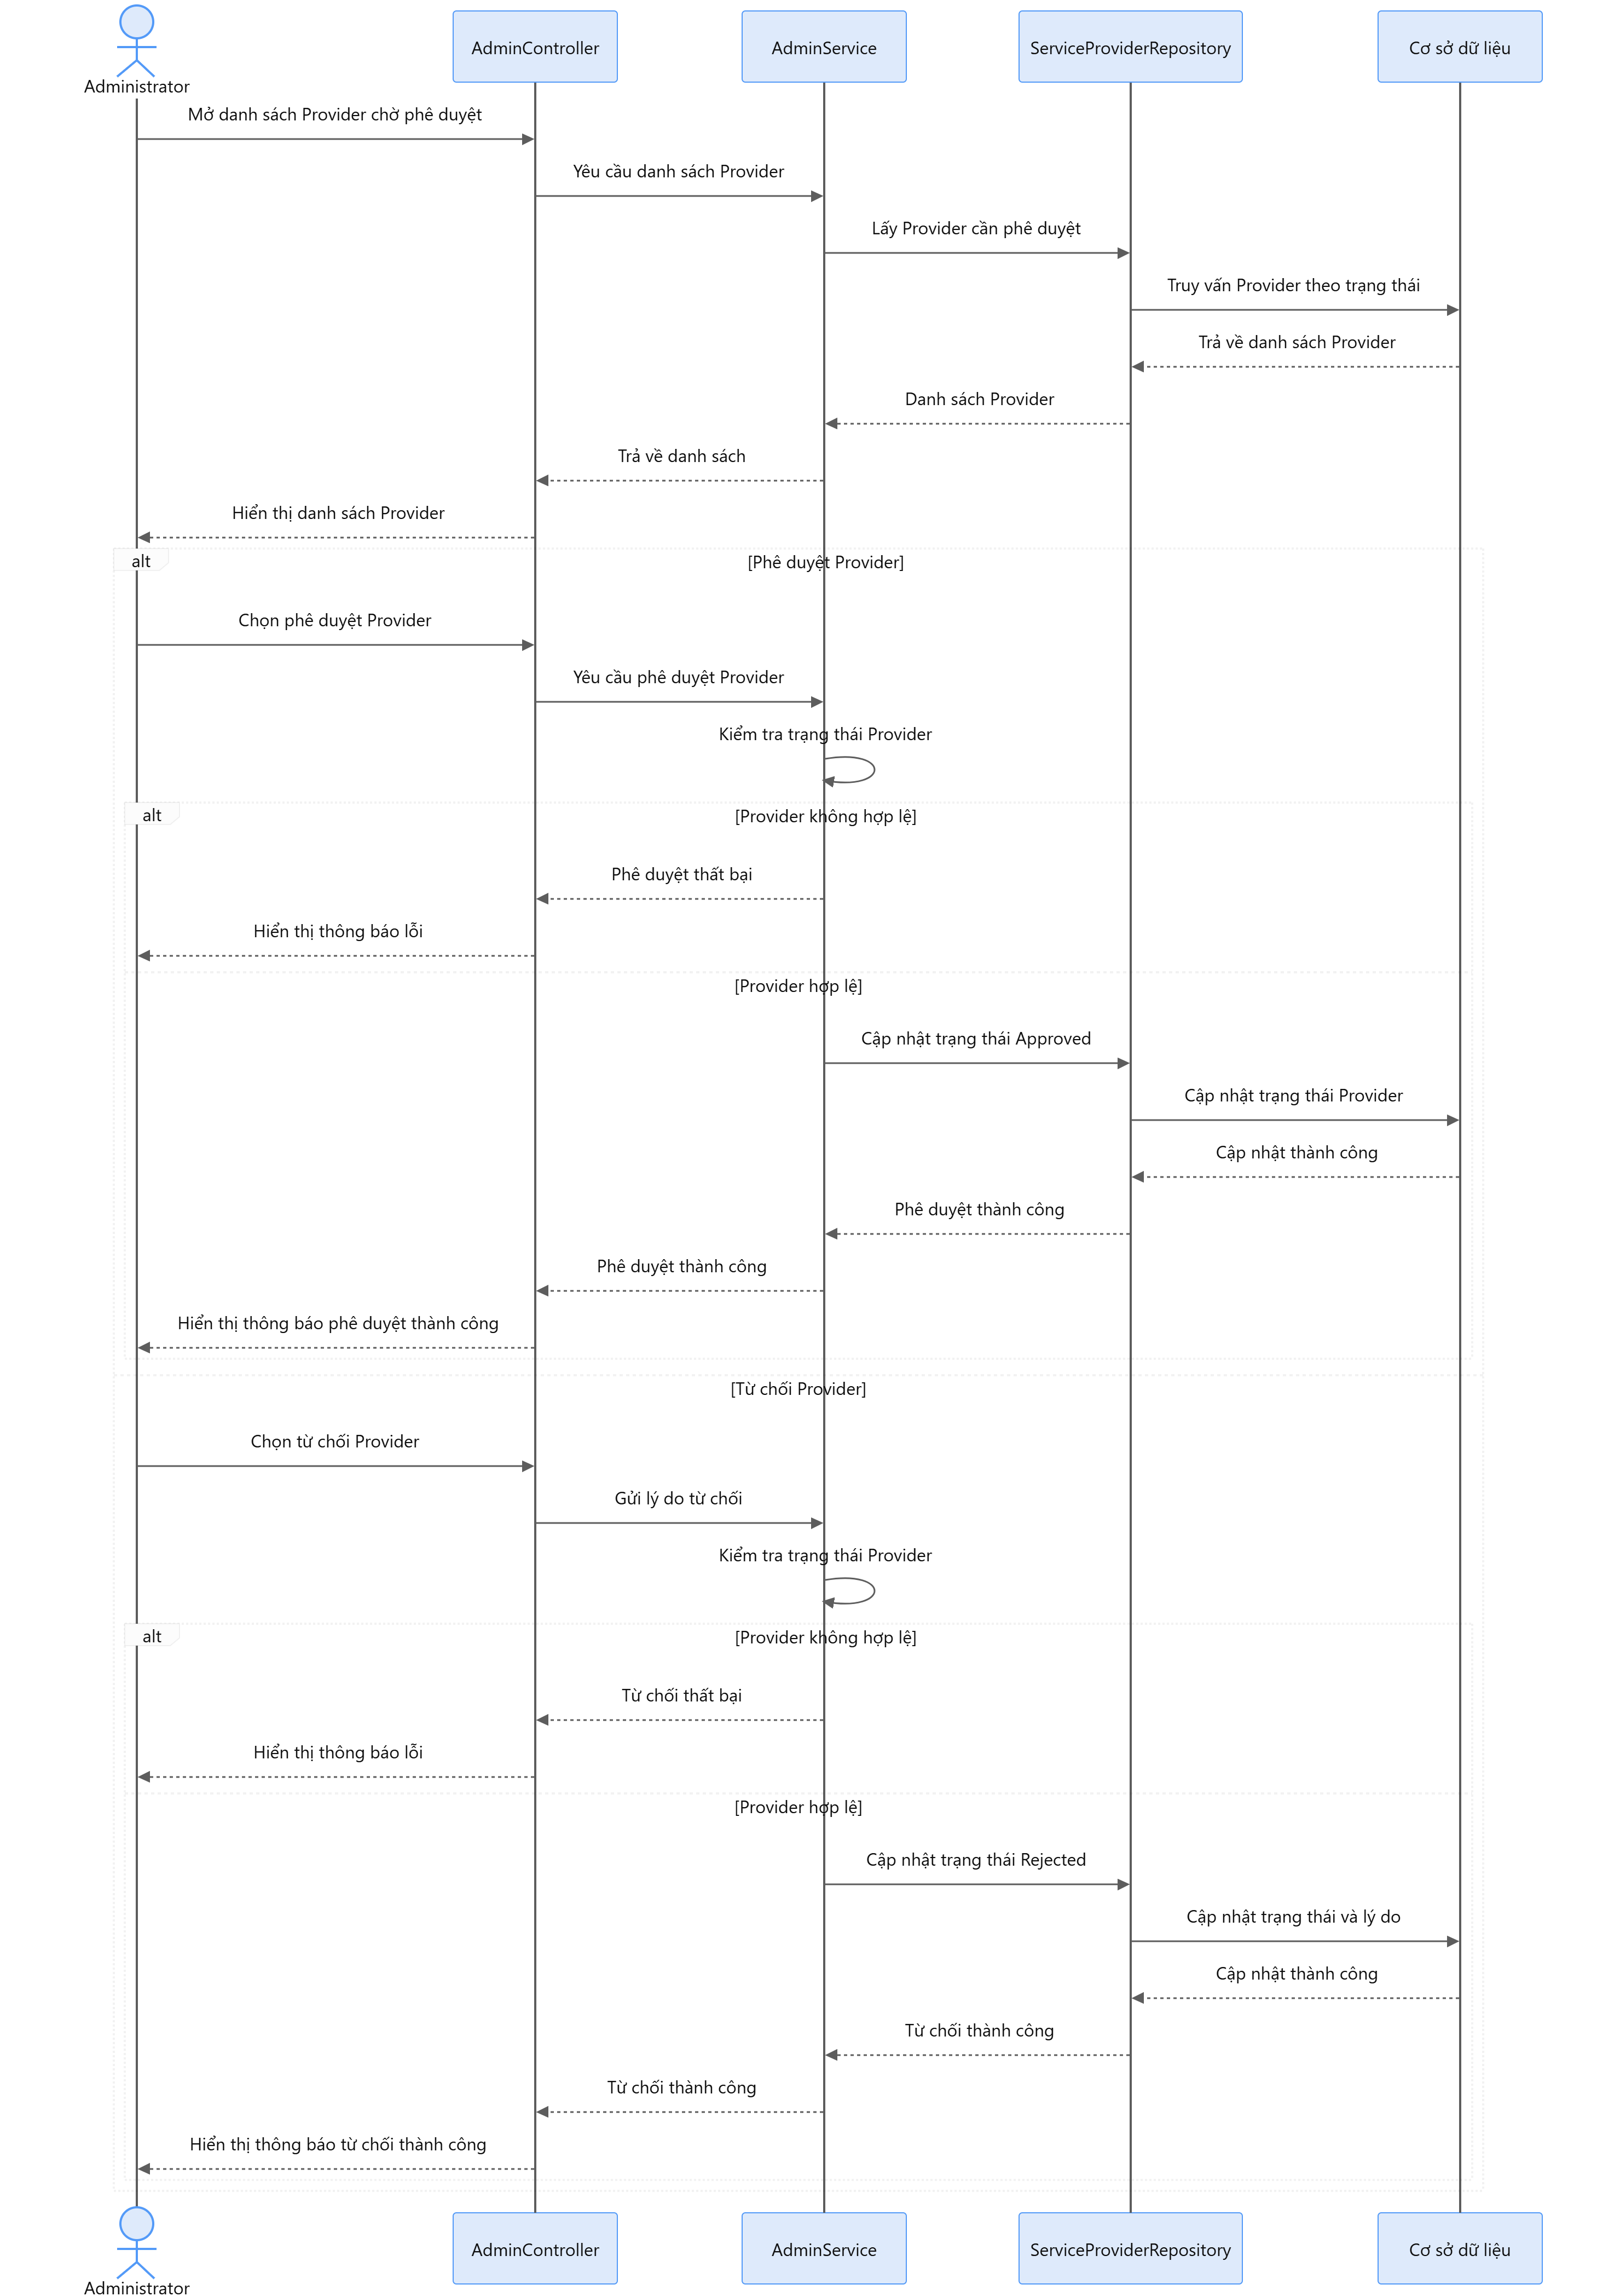
\includegraphics[width=1.1\textwidth]{images/53.png}
\end{figure}

	
	% ============================================================
	% CHAPTER V
	% TESTING
	% ============================================================
	
	\chapter{TÀI LIỆU KIỂM THỬ PHẦN MỀM}


\section{Phạm vi kiểm thử}

Phạm vi kiểm thử tập trung vào các chức năng chính của hệ thống kết nối cộng đồng nhiếp ảnh phim với các dịch vụ Darkroom và Studio đã được triển khai đầy đủ ở cả Frontend và Backend. Mục tiêu của kiểm thử là xác định hệ thống có hoạt động đúng theo yêu cầu chức năng hay không, dữ liệu có được xử lý chính xác hay không, đồng thời đảm bảo người dùng chỉ có thể thực hiện các chức năng phù hợp với vai trò của mình.

Hệ thống gồm ba tác nhân chính: Photographer, Service Provider và Administrator. Phạm vi kiểm thử được phân chia theo các nhóm chức năng của từng tác nhân.

\subsection{Các chức năng được kiểm thử}

Các chức năng sau được đưa vào phạm vi kiểm thử:

\begin{itemize}
	\item \textbf{Chức năng xác thực}
	\begin{itemize}
		\item Đăng ký tài khoản Photographer.
		\item Đăng nhập.
		\item Đăng xuất.
		\item Quên mật khẩu và xác thực bằng OTP.
		\item Đổi mật khẩu.
	\end{itemize}
	
	\item \textbf{Quản lý Photographer}
	\begin{itemize}
		\item Xem và cập nhật hồ sơ cá nhân.
		\item Tìm kiếm Creative Space.
		\item Xem chi tiết Creative Space.
		\item Đặt chỗ.
		\item Xem chi tiết Booking.
		\item Hủy Booking.
		\item Xem lịch sử Booking.
		\item Xem hóa đơn.
		\item Thanh toán Booking.
		\item Xem danh sách Workshop.
		\item Xem chi tiết Workshop.
		\item Đăng ký Workshop.
		\item Xem thông báo.
	\end{itemize}
	
	\item \textbf{Quản lý Service Provider}
	\begin{itemize}
		\item Xem và cập nhật hồ sơ Service Provider.
		\item Thêm, xem, cập nhật và xóa Creative Space.
		\item Thêm, xem, cập nhật và xóa Equipment.
		\item Thêm, xem, cập nhật và xóa Service Package.
		\item Xem và quản lý Booking.
		\item Xác nhận hoặc từ chối Booking.
		\item Thực hiện Check-in và Check-out.
		\item Thêm, xem, cập nhật và xóa Workshop.
		\item Xem danh sách người đăng ký Workshop.
		\item Xem Dashboard và thống kê.
		\item Quản lý thông tin thanh toán.
		\item Xem thông báo của Service Provider.
	\end{itemize}
	
	\item \textbf{Quản lý Administrator}
	\begin{itemize}
		\item Xem và quản lý người dùng.
		\item Xem và quản lý Service Provider.
		\item Phê duyệt hoặc từ chối Service Provider.
		\item Xem và quản lý giao dịch.
	\end{itemize}
\end{itemize}

\subsection{Các chức năng không thuộc phạm vi kiểm thử}

Các chức năng chưa được triển khai hoặc đã được loại bỏ khỏi phạm vi của hệ thống hiện tại không được đưa vào kiểm thử. Bao gồm:

\begin{itemize}
	\item Chức năng AI Assistant và các chức năng liên quan đến AI.
	\item Chức năng đăng bài và bình luận trong cộng đồng.
	\item Chức năng đánh giá và nhận xét.
	\item Chức năng quản lý khiếu nại.
	\item Chức năng hoàn tiền.
	\item Chức năng thay đổi lịch Booking.
	\item Chức năng quản lý bảo trì Equipment.
	\item Chức năng quản lý Consumable.
	\item Chức năng quản lý Package Detail độc lập.
\end{itemize}

Các chức năng trên được loại khỏi phạm vi kiểm thử vì không thuộc phạm vi chức năng được triển khai trong phiên bản hiện tại của hệ thống.

\subsection{Mức độ kiểm thử}

Quá trình kiểm thử được thực hiện ở ba mức độ chính:

\begin{itemize}
	\item \textbf{Kiểm thử đơn vị (Unit Testing):} tập trung kiểm tra từng thành phần riêng lẻ của Backend như Service, Repository, các hàm kiểm tra dữ liệu, xử lý xác thực, xử lý Booking và các hàm xử lý nghiệp vụ.
	
	\item \textbf{Kiểm thử tích hợp (Integration Testing):} kiểm tra sự tương tác giữa Frontend, các API của Backend, Service, Repository và cơ sở dữ liệu PostgreSQL. Mục tiêu là đảm bảo dữ liệu được gửi từ Frontend được Backend xử lý và lưu trữ hoặc truy xuất chính xác.
	
	\item \textbf{Kiểm thử hệ thống (System Testing):} kiểm tra toàn bộ hệ thống dưới góc nhìn của người sử dụng. Các luồng chức năng chính của Photographer, Service Provider và Administrator được kiểm tra để đảm bảo các module hoạt động đúng khi kết hợp với nhau.
\end{itemize}


% =========================================================
% 2. CHIẾN LƯỢC KIỂM THỬ
% =========================================================

\section{Chiến lược kiểm thử}

Chiến lược kiểm thử được xây dựng nhằm đảm bảo các chức năng đã triển khai hoạt động đúng và các thành phần của hệ thống có thể phối hợp với nhau một cách chính xác. Hoạt động kiểm thử tập trung vào yêu cầu chức năng, kiểm tra dữ liệu đầu vào, phân quyền người dùng, xử lý lỗi và các luồng nghiệp vụ chính.

\subsection{Các loại kiểm thử}

Hệ thống áp dụng các loại kiểm thử sau:

\begin{itemize}
	\item \textbf{Kiểm thử chức năng:} kiểm tra các chức năng của hệ thống có tạo ra kết quả đúng theo yêu cầu hay không.
	
	\item \textbf{Kiểm thử tích hợp:} kiểm tra sự kết nối và trao đổi dữ liệu giữa Frontend, Backend, các API, Service, Repository và cơ sở dữ liệu PostgreSQL.
	
	\item \textbf{Kiểm thử phân quyền:} kiểm tra quyền truy cập của ba vai trò Photographer, Service Provider và Administrator. Người dùng chỉ được phép truy cập và thực hiện các chức năng được phân quyền.
	
	\item \textbf{Kiểm thử dữ liệu đầu vào:} kiểm tra khả năng phát hiện và xử lý các dữ liệu không hợp lệ trong các chức năng như đăng ký, đăng nhập, cập nhật hồ sơ, đặt Booking, quản lý Creative Space, Equipment, Service Package và Workshop.
	
	\item \textbf{Kiểm thử xử lý lỗi:} kiểm tra hệ thống có trả về thông báo phù hợp khi dữ liệu không hợp lệ, dữ liệu không tồn tại, thông tin đăng nhập không chính xác hoặc người dùng thực hiện thao tác không được phép hay không.
	
	\item \textbf{Kiểm thử cơ sở dữ liệu:} kiểm tra dữ liệu được thêm, truy xuất, cập nhật và xóa chính xác trong PostgreSQL, đồng thời đảm bảo các mối quan hệ giữa các bảng được duy trì.
\end{itemize}

\subsection{Các mức độ kiểm thử}

\begin{longtable}{|>{\raggedright\arraybackslash}p{0.22\textwidth}|
		>{\raggedright\arraybackslash}p{0.34\textwidth}|
		>{\raggedright\arraybackslash}p{0.34\textwidth}|}
	\hline
	\textbf{Mức độ kiểm thử} &
	\textbf{Mục tiêu} &
	\textbf{Phạm vi chính} \\
	\hline
	
	Kiểm thử đơn vị &
	Kiểm tra từng thành phần và logic nghiệp vụ riêng lẻ của Backend. &
	Service, Repository, các hàm kiểm tra dữ liệu, xác thực, xử lý Booking và xử lý dữ liệu. \\
	\hline
	
	Kiểm thử tích hợp &
	Kiểm tra sự tương tác giữa các thành phần của hệ thống. &
	Frontend, API Flask, Service, Repository, PostgreSQL, xác thực, Booking, thanh toán, Workshop, Service Provider và Administrator. \\
	\hline
	
	Kiểm thử hệ thống &
	Kiểm tra toàn bộ hệ thống từ góc nhìn của người dùng. &
	Các luồng sử dụng của Photographer, Service Provider và Administrator. \\
	\hline
	
\end{longtable}

\subsection{Phương pháp kiểm thử}

Quá trình kiểm thử được thực hiện dựa trên các kịch bản sử dụng của từng chức năng. Đối với mỗi chức năng, dữ liệu hợp lệ và không hợp lệ được sử dụng để kiểm tra phản hồi của hệ thống.

Quy trình kiểm thử gồm các bước:

\begin{enumerate}
	\item Xác định chức năng cần kiểm thử và kết quả mong đợi.
	\item Chuẩn bị dữ liệu đầu vào hợp lệ và không hợp lệ.
	\item Thực hiện chức năng thông qua giao diện Frontend hoặc API tương ứng.
	\item Kiểm tra phản hồi được trả về từ Backend.
	\item Kiểm tra kết quả hiển thị trên giao diện Frontend.
	\item Kiểm tra dữ liệu trong cơ sở dữ liệu đối với các chức năng có thay đổi dữ liệu.
	\item Kiểm tra quyền truy cập tương ứng với vai trò của người dùng.
	\item Ghi nhận kết quả quan sát được để phục vụ việc tổng hợp kết quả kiểm thử.
\end{enumerate}

\subsection{Công cụ hỗ trợ kiểm thử}

Các công cụ được sử dụng để hỗ trợ quá trình kiểm thử bao gồm:

\begin{itemize}
	\item \textbf{Trình duyệt Web:} sử dụng để thực hiện kiểm thử các chức năng thông qua giao diện Frontend.
	
	\item \textbf{Developer Tools:} sử dụng để kiểm tra hoạt động của Frontend, các request và response API, thông tin Network và các lỗi phía Client.
	
	\item \textbf{Postman:} sử dụng để kiểm thử trực tiếp các REST API của Backend, kiểm tra request, response, xác thực và phân quyền.
	
	\item \textbf{PostgreSQL / Supabase:} sử dụng để kiểm tra dữ liệu trong cơ sở dữ liệu, các bản ghi được tạo hoặc cập nhật sau khi thực hiện chức năng.
	
	\item \textbf{Visual Studio Code:} sử dụng để kiểm tra và hỗ trợ quá trình sửa lỗi trong mã nguồn Frontend và Backend.
\end{itemize}


% =========================================================
% 3. KẾ HOẠCH KIỂM THỬ
% =========================================================

\section{Kế hoạch kiểm thử}

Kế hoạch kiểm thử xác định các nguồn lực, môi trường và các giai đoạn cần thiết để kiểm tra hệ thống. Hoạt động kiểm thử được thực hiện dựa trên phạm vi chức năng và chiến lược kiểm thử đã trình bày ở các phần trước.

\subsection{Nhân sự kiểm thử}

Hoạt động kiểm thử được thực hiện bởi các thành viên trong nhóm phát triển. Các thành viên tham gia kiểm thử dựa trên các module và chức năng mà nhóm đã triển khai.

Các công việc chính trong quá trình kiểm thử bao gồm:

\begin{itemize}
	\item Chuẩn bị dữ liệu kiểm thử cho các chức năng.
	\item Thực hiện kiểm thử chức năng thông qua giao diện Frontend.
	\item Kiểm thử các API của Backend và kiểm tra kết quả trả về.
	\item Kiểm tra dữ liệu trong cơ sở dữ liệu sau các thao tác thêm, cập nhật và xóa.
	\item Kiểm tra phân quyền giữa Photographer, Service Provider và Administrator.
	\item Phát hiện và ghi nhận các lỗi trong quá trình kiểm thử.
	\item Kiểm tra lại các chức năng sau khi lỗi được sửa.
\end{itemize}

\subsection{Môi trường kiểm thử}

Môi trường kiểm thử bao gồm Frontend, Backend và cơ sở dữ liệu PostgreSQL của hệ thống.

\begin{longtable}{|>{\raggedright\arraybackslash}p{0.25\textwidth}|
		>{\raggedright\arraybackslash}p{0.65\textwidth}|}
	\hline
	\textbf{Thành phần} & \textbf{Môi trường kiểm thử} \\
	\hline
	
	Frontend &
	Ứng dụng Web được xây dựng bằng HTML, CSS và JavaScript, được truy cập thông qua trình duyệt Web. \\
	\hline
	
	Backend &
	Backend được xây dựng bằng Flask theo kiến trúc Clean Architecture, bao gồm các Controller, Service, Repository và Model. \\
	\hline
	
	Cơ sở dữ liệu &
	Sử dụng PostgreSQL để lưu trữ dữ liệu của hệ thống như Users, Roles, ServiceProviders, CreativeSpaces, Bookings, Payments, Workshops và Notifications. \\
	\hline
	
	Kiểm thử API &
	Sử dụng Postman để gửi request đến các REST API và kiểm tra request, response, xác thực, phân quyền và dữ liệu trả về. \\
	\hline
	
	Kiểm thử giao diện &
	Sử dụng trình duyệt Web và Developer Tools để kiểm tra giao diện, request API, response và các lỗi phía Client. \\
	\hline
	
\end{longtable}

\subsection{Các mốc kiểm thử}

Hoạt động kiểm thử được chia thành các mốc chính nhằm đảm bảo các nhóm chức năng quan trọng được kiểm tra trước khi hoàn thiện hệ thống.

\begin{longtable}{|>{\raggedright\arraybackslash}p{0.18\textwidth}|
		>{\raggedright\arraybackslash}p{0.32\textwidth}|
		>{\raggedright\arraybackslash}p{0.38\textwidth}|}
	\hline
	
	\textbf{Mốc kiểm thử} &
	\textbf{Hoạt động} &
	\textbf{Kết quả mong đợi} \\
	\hline
	
	Mốc 1 &
	Kiểm thử chức năng xác thực &
	Kiểm tra đăng ký, đăng nhập, đăng xuất, quên mật khẩu và đổi mật khẩu. \\
	\hline
	
	Mốc 2 &
	Kiểm thử chức năng Photographer &
	Kiểm tra quản lý hồ sơ, tìm kiếm và xem Creative Space, Booking, hủy Booking, thanh toán, Workshop và thông báo. \\
	\hline
	
	Mốc 3 &
	Kiểm thử chức năng Service Provider &
	Kiểm tra hồ sơ Provider, Creative Space, Equipment, Service Package, Booking, Workshop, thông tin thanh toán, Dashboard và thông báo. \\
	\hline
	
	Mốc 4 &
	Kiểm thử chức năng Administrator &
	Kiểm tra quản lý người dùng, quản lý Service Provider, phê duyệt Service Provider và quản lý giao dịch. \\
	\hline
	
	Mốc 5 &
	Kiểm thử tích hợp và kiểm thử hệ thống &
	Kiểm tra các luồng chức năng có sự kết hợp giữa Frontend, Backend, cơ sở dữ liệu, xác thực và phân quyền. \\
	\hline
	
	Mốc 6 &
	Kiểm tra hoàn thiện &
	Kiểm tra lại các chức năng sau khi sửa lỗi và xác nhận hệ thống sẵn sàng cho quá trình hoàn thiện và bàn giao. \\
	\hline
	
\end{longtable}


	
	% ============================================================
	% CHAPTER VI
	% RELEASE
	% ============================================================
	
	\chapter{GÓI PHÁT HÀNH VÀ HƯỚNG DẪN SỬ DỤNG}

\section{Deliverable Package}

\begin{longtable}{|c|p{4cm}|p{8cm}|}
	\hline
	\textbf{No.} & \textbf{Deliverable Item} & \textbf{Description} \\ 
	\hline
	1 & Schedule/Task Tracking &
	Sử dụng Jira để theo dõi tiến độ thực hiện các công việc của dự án và quản lý các task của từng thành viên. \\
	\hline
	
	2 & Project Backlog &
	Sử dụng Jira để quản lý Product Backlog, phân chia các chức năng thành các task và theo dõi trạng thái thực hiện của từng task. \\
	\hline
	
	3 & Source Codes &
	Mã nguồn của hệ thống được quản lý và lưu trữ trên GitHub, bao gồm:
	\begin{itemize}
		\item Back End: Flask Clean Architecture
		\item Front End: Web application sử dụng HTML, CSS và JavaScript
	\end{itemize}
	\\
	\hline
	
	4 & Database Script(s) &
	Các script SQL được sử dụng để tạo và quản lý cơ sở dữ liệu PostgreSQL của hệ thống. Cơ sở dữ liệu được triển khai trên Supabase. \\
	\hline
	
	5 & Final Report Document &
	Tài liệu báo cáo cuối kỳ tổng hợp các nội dung của dự án, bao gồm phân tích yêu cầu, thiết kế hệ thống, cơ sở dữ liệu, kiểm thử và hướng dẫn sử dụng. \\
	\hline
	
	6 & Test Cases Document &
	Tài liệu mô tả phạm vi, chiến lược và kế hoạch kiểm thử cho các chức năng của hệ thống. \\
	\hline
	
	7 & Slide &
	Tài liệu trình chiếu giới thiệu dự án, bao gồm thành viên nhóm, actors, bối cảnh dự án, công nghệ sử dụng, yêu cầu chức năng, yêu cầu phi chức năng và các luồng chức năng chính của hệ thống. \\
	\hline
	
\end{longtable}

\section{Hướng dẫn cài đặt}

\subsection{Yêu cầu hệ thống}

\subsubsection{Web Application}

\begin{longtable}{|p{4cm}|p{5cm}|p{5cm}|}
	\hline
	\textbf{Component} & \textbf{Minimum} & \textbf{Recommended} \\
	\hline
	CPU & Intel Core i5 & Intel Core i7 \\
	\hline
	Memory & 8GB RAM & 16GB RAM trở lên \\
	\hline
	Storage Space & 10GB trống & 20GB trống \\
	\hline
	Network & 10 Mbps & 50 Mbps trở lên \\
	\hline
	Web Browser & Chrome phiên bản mới & Chrome phiên bản mới nhất \\
	\hline
\end{longtable}

\subsection{Hướng dẫn cài đặt}

\subsubsection{Backend}

\textbf{Step 1:} Cài đặt Visual Studio Code.

\textbf{Step 2:} Cài đặt Git.

\textbf{Step 3:} Clone source code Backend từ GitHub.

\textbf{Step 4:} Mở thư mục Backend bằng Visual Studio Code.

\textbf{Step 5:} Tạo và kích hoạt môi trường ảo Python.

\textbf{Step 6:} Cài đặt các thư viện cần thiết.

\textbf{Step 7:} Cấu hình thông tin kết nối cơ sở dữ liệu PostgreSQL.

\textbf{Step 8:} Chạy Backend.

\subsubsection{Frontend}

\textbf{Step 1:} Mở thư mục Frontend bằng Visual Studio Code.

\textbf{Step 2:} Kiểm tra cấu hình kết nối với Backend.

\textbf{Step 3:} Mở Terminal tại thư mục Frontend.

\textbf{Step 4:} Chạy Frontend bằng trình duyệt web.

\textbf{Step 5:} Truy cập địa chỉ của ứng dụng trên trình duyệt.
\section{Hướng dẫn sử dụng}

\subsection{Tổng quan}

% Liệt kê chức năng theo Photographer / Service Provider / Administrator

\subsection{Hướng dẫn chức năng}

\subsubsection{Đăng ký tài khoản}
	
	% ============================================================
	% END DOCUMENT
	% ============================================================
	
\end{document}

